\ifsvnmulti
 \svnkwsave{$RepoFile: lyapunov/XiongDing.tex $}
 \svnidlong {$HeadURL: svn://zero.physics.gatech.edu/siminos/lyapunov/XiongDing.tex $}
 {$LastChangedDate: 2017-03-29 23:38:45 -0400 (Wed, 29 Mar 2017) $}
 {$LastChangedRevision: 5740 $} {$LastChangedBy: xiong $}
 \svnid{$Id: XiongDing.tex 5740 2017-03-30 03:38:45Z xiong $}
\fi

\chapter{Xiong Ding's project}
\label{sect:introXD}

\begin{bartlett}{
Sometimes a scream is better than a thesis.
                }
\bauthor{
Ralph Waldo Emerson
        }
\end{bartlett}

\bigskip

The goal of the summer/fall 2013 project is that \XD\ adopts the Ginelli
\etal\rf{GiChLiPo12} method for computation of {\cLvs} to
computation of \po\ Floquet vectors,  and implement it for the \po s and
\rpo s in our \KS\ database.


\begin{description}

\item[2013-06-27 Predrag] Our first goal is to learn
how to compute \emph{all} eigenvectors (CLVs) and Floquet multipliers
(in literature mistakenly often called `Lyapunov exponents') of
\JacobianMs\ for \po s computed in \refref{SCD07}.
Please study this reference in depth. For \KS\
calculations of \refchap{sect:LyapKS}, system size $L=22$, this is 62
eigenvectors. We have at least 40,000 \rpo s.

%fine tuned 2013-08-02
You will first check whether your numerical code for \jacobianM\
integration
\beq
 \frac{d}{dt}J^t=A J^t \quad J^0=I
\ee{XD-JacobianEq}
reproduces the analytic eigenvalue and eigenvector
linear stability spectrum for the simplest \eqv\ solution $u(x)=0$. Next
you will check how well do you compute the stability exponents for the
three numerical \eqva\ and the two \rpo s of section {\em 2.2.
Equilibria and relative equilibria}
 of \refrefs{SCD07}.

Then you will check
whether you agree with Kazumasa's results for his
favorite \po\ \PO{10.3} with $\period{p} = 10.253$.
\PO{10.3} is the prime orbit period of a pre-\po,
the full period is twice that, see Fig. 6.1\,(i) \emph{Selected
relative periodic and pre-\po s} in \refref{SCD07}.


%fine tuned 2013-08-02
Now the new work starts. What is clearly dumb about the numerical
method described in Francesco
    \etal\ review paper\rf{GiChLiPo12} is that one mindlessly
    integrates the \jacobianM\  $\jMps^\zeit$
for arbitrarily long times, but for the invariant solutions \emph{no}
time integration is needed (\eqva), or \emph{only one time period}
\period{} integration is needed (\po s).
\\(Kazz) This is true, but as you know, Ginelil's algorithm was
invented to study chaotic systems. Therefore, application of Ginelli's
method to fixed points or periodic orbits (if they do) should only be
meant to compare with Floquet eigenexponents and eigenvectors. They
(including me in the same group) are not so dumb...

Your project is to rethink the linear algebra of \refref{GiChLiPo12}
so that you can compute all stability eigenexponents and eigenvectors
of $\jMps^\zeit$ for a numerically given \eqv\ solution,
\emph{without} the mindless time integrations.
It should not be too hard :). The reasons why it has not been done
because all the people involved so far are happiest running long-time
mindless simulations.
\PCedit{ %fine tuned 2013-08-05
But I might be too flippant here:
    }
fluid dynamicists (see for example
Appendices \HREF{http://www.cns.gatech.edu/~predrag/papers/steady.pdf}
{A.2 and A.3} in \refref{GHCW07}) do compute stability of \eqva\ using
time integration and Krylov spaces...

Save your code in a \texttt{siminos/xiong/} subfolder. You want to
confirm the result in \refref{SCD07}, see
\HREF{http://www.cns.gatech.edu/~predrag/papers/SCD07.pdf}{sect. 4} in
that paper:
    \PC{the source file is in \texttt{siminos/rpo\_ks/}}

\begin{quote}
``[...] Indeed, numerically the {\cLvs}\rf{ginelli-2007-99} of the $L=22$ chaotic attractor separate
into 8 ``physical'' vectors with small Lyapunov exponents
$(\Lyap_j) = (0.048,$ 0, 0, $-0.003$, $-0.189$, $-0.256$,
$-0.290$, $-0.310$),
and the remaining 54 ``hyperbolically isolated'' vectors with rapidly
decreasing exponents
$(\Lyap_j)
= (-1.963$,   $-1.967$,   $-5.605$,   $-5.605$,  $-11.923$,  $-11.923$,
 $\cdots) \approx -(j/\tildeL)^4$,
in full agreement with the Yang \etal\rf{YaTaGiChRa08} investigations
of KS for large systems sizes.
 [...]''
\end{quote}

\item[2013-06-27 Predrag]
This section up to \refsect{sect:dailyBlXD} are an evolving draft of
\XD\'s project report; daily progress is reported in
\refsect{sect:dailyBlXD}~{\em Daily blog}.

Please {\color{red} write down here}, in your project's
log, the equations you are integrating (you can clip and paste
equations from elsewhere in this repository to save time).
This will be a continuously evolving draft of the project report.
When you
write up the project report it will all be needed, so you might just
as well do it now.

If we know where are you in the project, we can help you.
Write up full fledged
derivations and explanations of what you are learning - clear enough
that some of that text can be later used in your project report, or a
publication, if we get that far. Clear exposition is 1/3 of research.

My vision of the project is sketched in \refchap{c-draft}. Studying
\refchap{s:LyapunovVec} is also a good idea. \refChap{sect:LyapKS}
deals specifically with the \KS\ calculations.
Search for\\
``2012-02-06 Evangelos Talked with Hugues at MPIPKS, created a to-do list:''
\\
to see Evangelos and Hugues work plan.

\item[2013-06-27 Predrag]
Setting up \XD\ for the svn (subversion) repository access

\texttt{svn://zero.physics.gatech.edu/siminos}

you will
need this userID, password, so save it in your secret stash of magic
words:
\\
user: xiong  password: Lyapunov

to access repositories read about subversion/svn and VPN access on
\HREF{http://cns.gatech.edu/CNS-only} {cns.gatech.edu/CNS-only} - to
access any of the internal CNS pages you will need

cnsuser           cnsweb

\HREF{http://ChaosBook.org/library}{Click here} for internal reprints and
books collection. You will need

student           Lautrup

I do not have the patience to enter every paper in the listing on this
internal home page, so many papers are there but not listed. Their PDF
file name is the same as their bibTeX name for the publication. For
example, a book by Wassim M. Haddad\rf{HaCh08} has BibTeX name
\texttt{HaCh08}, so I put a copy of their book into the
ChaosBook.org/library as

\HREF{http://ChaosBook.org/library/HaCh08.pdf}
{ChaosBook.org/library/HaCh08.pdf}.

If you download some publications that would be nice to save for other
people, let me know, and I'll show you how to do it.

To compile the blog,
\begin{verbatim}
 cd siminos/lyapunov/
 pdflatex blog; bibtex blog; pdflatex blog
\end{verbatim}

To help a bit with starting writing, I will
edit your text (you can see edits by using diff in Tortoise).

Here is how you can
\Xiongedit{highlight your edits}, and here is how you can add a dated
footnote\Xiong{2013-03-03}{This is a footnote. Always enter the date, so
we know how old it is.}.

In the first draft, do not worry about
English, just focus on the formulas. Write
down what a starting graduate student would need to know to be able
to set up the calculation.

If you want source files for ChaosBook.org to clip and past from, you can
\begin{verbatim}
  svn checkout svn:\\zero.physics.gatech.edu\dasbuch
\end{verbatim}

Always trim the figures, avoid lots of white
space around the edges.

If you look into directory
siminos/chaos/ and pdflatex blog.tex, you can see an example of what
a student work log looks like (after a semester of so of work).
For examples of
what final reports look like, see \wwwcb{/projects}.

Come to me or Skype me if there is something you
cannot figure out.

\item[2014-10-27 Predrag]
to Xiong Ding: in the future, please diff my edits of your siminos.bib
entries, so not to make same errors again and again. We use
\begin{itemize}
  \item abbreviations, not full journal names
  \item initials, not full person names
  \item page numbers, volume numbers
  \item doi without \texttt{http://}
  \item chapter in a collection is not cited as an article with the title of
         the book cited as `journal'
\end{itemize}
If the bibliography is messy, the reader will assume that the article
itself is not proofread either, and thus not trustworthy.
\end{description}

    \newpage
\ifsvnmulti
 \svnkwsave{$RepoFile: lyapunov/xiong/blog/CovVecs.tex $}
 \svnidlong {$HeadURL: svn://zero.physics.gatech.edu/siminos/xiong/blog/CovVecs.tex $}
 {$LastChangedDate: 2016-03-01 08:25:36 -0500 (Tue, 01 Mar 2016) $}
 {$LastChangedRevision: 4663 $} {$LastChangedBy: predrag $}
 \svnid{$Id: CovVecs.tex 4663 2016-03-01 13:25:36Z predrag $}
\fi

\section{\CLvs}
\label{sect:CovVecs}

\begin{description}

\item[2013-06-27 Predrag]
I rewrote ChaosBook.org chapters
\HREF{http://chaosbook.org/paper.shtml\#stability} {``Linear stability''},
\HREF{http://chaosbook.org/paper.shtml\#invariants} {``Cycle
stability''}, and
\HREF{http://chaosbook.org/paper.shtml\#Lyapunov} {``Lyapunov
exponents''}, to help graduate students. Any suggestion for improving
these chapters is greatly appreciated.

                              \inCB
{Finite-time} {Lyapunov} or \emph{characteristic} exponents and
associated \emph{principal axes} in the theory of dynamical systems
are discussed in chapter
\HREF{http://chaosbook.org/paper.shtml\#Lyapunov} {``Lyapunov
exponents''}. Oseledec \emph{Lyapunov exponents}\rf{lyaos} are the
$\zeit\to\infty$ limit of these. \emph{Floquet multipliers} and
\emph{eigen-vectors} are property of finite-time, compact invariant
solutions, such as \po s and \rpo s; they are explained in chapter
\HREF{http://chaosbook.org/paper.shtml\#invariants} {``Cycle
stability''}. \emph{Stability exponents}\rf{GoSuOr87} are the
corresponding long-time limit, and --in one of those frustrating
historical accidents-- the corresponding
\emph{stability} eigenvectors are misnamed in recent papers
\emph{Lyapunov vectors}, even though \emph{they are not} the
eigenvectors that correspond to the Lyapunov exponents. Sorry, not my
fault. The prefix `covariant' is meant to distinguish the two kinds of
eigenvectors. That's just confusing, for no good reason - Lyapunov
has nothing to do with linear stability described by the \jacobianM\
$\jMps$, as far as I know his paper\rf{Lyap1892}
is about $(\transp{\jMps}\!\jMps)$ and the associated principal axes.

Oseledec proofs are important in mathematics, but not
sensible for computational work in dynamical systems. For me the
Goldhirsch, Sulem and Orszag\rf{GoSuOr87} exposition is the clearest
(read it \HREF{http://chaosbook.org/library/GoSuOr87.pdf}{here}).
They correctly distinguish \emph{Lyapunov} eigenvalues and eigenvectors
from the \emph{stability} eigenvalues and eigenvectors.

At that time Goldhirsch \etal\ had no proof that the long-time Lyapunov
exponents converge to the stability exponents (Kazumasa, do you have
some more recent paper that you prefer to Goldhirsch \etal?).

Trevisan and Pancotti\rf{TrePan98} \emph{Periodic orbits, Lyapunov
vectors, and singular vectors in the Lorenz system} (see above, read it
\HREF{http://chaosbook.org/library/TrePan98.pdf}{here})) apparently need
to be cited for the observation that {\cLvs} reduce to Floquet
eigenvectors in the particular case of a {\po}. Seems so obvious it is in
ChaosBook without attribution, and Ruelle and
Eckmann\rf{EckmannRuelle1985} surely say the same (though I have not
checked). Most importantly for our project, they say:

``The leading Lyapunov vectors, as defined here, as well as the
asymptotic final singular vectors, are tangent to the attractor,
while the leading initial singular vectors, in general, point away
from it. Perturbations that are on the attractor can be found in the
subspace of the leading Lyapunov vectors.''

They have very nice pictures for Lorenz unstable orbits illustrating that.

\item[2013-06-27 Predrag]
Graduate students are brave people who immediately jump into the deep
end of the pool, without any testing. Here are two 2\dmn\ maps, the
Lozi map (for $a=1.85, b=0.3$)
% \PC{need figure of Lozi strange attractor}
\bea
   x_{n+1} &=& 1-a |x_{n}|+ b y_n  \continue
   y_{n+1} &=& x_{n}
\,,
\label{e_lozi_def}
\eea
and the H\'enon map (for $a=1.4, b=0.3$; described at length in
\refchap{c-Henon})
\bea
    x_{n+1}&=&1-ax^2_n+b y_n
        \continue
    y_{n+1}&=& x_n
\,,
\label{eq2.1d}
\eea
for which fixed points are available analytically\rf{DasBuch} (for
the Lozi map all periodic points are available analytically). So see
what Floquet exponents
your program returns for \po s of these humble maps, and then for
ergodic trajectories, before running the programs on ergodic
trajectories in zillion dimensions.

If your programs only apply to continuous time flows (ODEs rather
than maps), ChaosBook\rf{DasBuch} has \eqva\ and \po s for 2\dmn\
Lorenz and R\"ossler flows, and Evangelos has lots of \rpo s for the
\cLe; make sure your programs work on small systems first.

\end{description}

    \newpage
\ifsvnmulti
 \svnkwsave{$RepoFile: xiong/blog/CLVs.tex $}
 \svnidlong {$HeadURL: svn://zero.physics.gatech.edu/siminos/xiong/blog/CLVs.tex $}
 {$LastChangedDate: 2014-10-01 10:41:30 -0400 (Wed, 01 Oct 2014) $}
 {$LastChangedRevision: 3707 $} {$LastChangedBy: xiong $}
 \svnid{$Id: CLVs.tex 3707 2014-10-01 14:41:30Z xiong $}
\fi

% --------------------------------------------------------
\subsection{Oseledec splitting}
\label{sect:CLVs}

\begin{description}
  
\item[2013-09-04 \XD] Notes on the Ginelli \etal\
  method\rf{GiChLiPo12}, \arXiv{1212.3961}.

\item[2013-09-18 \XD]
  I didn't read Oseledec\rf{lyaos}. I try to summarize the basic ideas
  of \refref{GiChLiPo12}, which are also abstract to me.

\item[2014-09-30 \XD]
  I tried to study the Oseledec splitting again, and find that my 
  previous understanding is wrong, but the notes here may be helpful
  for me in future. I will rewrite my understanding in the next 
  subsection.

\end{description}


 Let $f^{k}(x) : \pS \mapsto \pS$ be a measure preserving map in \statesp\ \pS. Every point
 in this $\pS$ is a vector $x_{t}=(x_{t}^{(1)},x_{t}^{(2)},\dots,x_{t}^{(N)})\in \mathbb{R}^N$,
 where the subscript $t$ denotes instant time. If time is discretized
 $t=k\Delta t,\quad k=0,1,2...$ , then we can define Jacobina
 matrix of this system as
 $M_{k,n}=M^{k\Delta t}(x_n)=\frac{\partial{f(x_{(n+k)\Delta t})}}{\partial{x_{n\Delta t}}}$.
 Therefore, $M_{k,n}$ evolves the tangent space forward $k$ time steps from a point in tangent
 space $\delta x_n$.

    \PC{2013-09-15 Define dimension of \statesp\ \pS, you use it later.\\
    Xiong-2013-09-18: You are
    right. I define the space to be N-dimensional.}
    \PC{2013-09-15 What measure? Why measure preserving?\\
    Xiong-2013-09-18: For this one, I don't
    know the answer. I will update my opinion later.}
    \PC{2013-09-15 Index $n$ in $M_{k,n}$ means what? A pair of matrix indices,
    action on a vector $\ssp \in \pS$? To me it looks like the initial time is $n$,
    the \jacobianM\ is evaluated $k$ time steps later. Otherwise it would be stupid
    to have that index ${}_n$ on everything that follows.\\
    Xiong-2013-09-18: Yes, you are
    right. It is my mistake.}


 If the mapping is invertible, then we have several statements.

 \begin{itemize}
  \item forward/backward Oseledec matrix:
    \[
     \Xi^{\pm}= \lim_{k\to \pm \infty} \frac{1}{2k} \ln [M_{k,n}^{\dagger}M_{k,n}]
    \]
     exits.

  \item $\Xi^{\pm}$ share the same eigenvalues
  $\lambda_{n}^{(1)}> \lambda_{n}^{(2)}> \dots \lambda_{n}^{(m)}$.
      \PC{2013-09-15 If I reverse dynamics, and go $k\to - \infty$, shouldn't all these
      exponents change sign?\\
      Xiong-2013-09-18: Yes. If you reverse dynamics, the exponents of Jacobian
      matrix will change sign. But
      the definition of forward Oseledec matrix is the
      product of two Jacobian matrices. $M_{k,n}^{\dagger}$ evolves the system backward
      and $M_{k,n}$ evolves system forward, so forward Oseledec matrix will evolve system
      forward first and then backward, which consists two processes. Similarly, backward Oseledec
      martrix evolves the system backward first and then forward. For me, the definition
      of forward/backward Oseledec matrix is time invertible. I am not sure about this point since
      I don't know
      how mathmaticians proved this theorem.}

  The corresponding eigenspaces are
  $(U_{n}^{(1)})^{\pm}, (U_{n}^{(2)})^{\pm}, \dots (U_{n}^{(m)})^{\pm} $,
  with degeneracies
  $m_{n}^{(i)}=dim (U_{n}^{(i)})^{\pm}$. Also, we define Oseledec subspaces as
    \PC{2013-09-15 Are you saying there are $i$ positive $\lambda_{n}^{(\ell)}$,
    rest are negative? Have you assumed $\lambda_{n}^{(\ell)}\neq 0$?
    Why is $(U_{n}^{(i)})^{+}$ shared? Why is in $(T_{n}^{(i)})^{-}$?\\
    Xiong-2013-09-18: I am not assuming that there are $i$ positive exponents, nor
    they cannot be zero. I just want to construct a subspace $(T_{n}^{(i)})^{+}$
    which is spaned by the last $m-i+1$ eigenspaces of the forward Oseledec matrix, and
    a subspace $(T_{n}^{(i)})^{-} $ which is spaned by the first $i$ eigenspaces of the
    backward Oseledec matrix. So
    for each vector $u\in (T_{n}^{(i)})^{\pm}\backslash (T_{n}^{(i\pm 1)})^{\pm}$:
    \[
     \lim_{k\to \pm \infty} \frac{1}{k} \ln \frac{\| M_{k,n}u \|}{\| u \|} =\lambda_{n}^{(i)}
    \]
     by the way,
     \[
     \lim_{k\to \pm \infty} \frac{1}{|k|} \ln \frac{\| M_{k,n}u \|}{\| u \|} =\pm \lambda_{n}^{(i)}
    \]
    $(U_{n}^{(i)})^{+}$ is not included in the definition of $(T_{n}^{(i)})^{-}$. Sorry for my typo.
    }
  \begin{align}
   (T_{n}^{(i)})^{+} &= (U_{n}^{(i)})^{+} \oplus \dots \oplus (U_{n}^{(m)})^{+}\\
   (T_{n}^{(i)})^{-} &= (U_{n}^{(1)})^{-} \oplus \dots \oplus (U_{n}^{(i)})^{-}
   \label{eq::xiong_back}
  \end{align}
  The forward Oseledec subspace covers the space
  spanned by the eigenvectors corresponding
  to \PCedit{negative} eigenvalues; while, the backward Oseledec subspace
  covers the space spanned by the eigenvectors corresponding to
  \PCedit{positive} eigenvalues.

  Then, we have the following identity:
  \begin{align}
   &\lim_{k\to \pm \infty} \frac{1}{k} \ln \frac{\| M_{k,n}u \|}{\| u \|}  \\
   &=\lim_{k\to \pm \infty} \frac{1}{2k} \ln \frac{u^{\dagger}[M_{k,n}^{\dagger}M_{k,n}]u}{u^{\dagger} u}\\
   &=\frac{u^{\dagger}\Xi^{\pm}u}{u^{\dagger} u}\\
   &=\lambda_{n}^{(i)}
  \end{align}
  for $u\in (T_{n}^{(i)})^{\pm} \backslash (T_{n}^{(i\pm 1)})^{\pm}$

  This is the definition of Covariant Lyapunov Exponents. For
  ergodic system, these exponents are flow invariant,
  % which means that they don't depend on there positions.
  \PCedit{\ie, they almost always do not depend on the initial point $\ssp$
  at time $n$}.
    \PC{2013-09-15 not true if $\ssp$ is a fixed or periodic point.}
  \item Oseledec splitting is defined as

  \begin{equation}
   \Omega_{n}^{(i)}=(T_{n}^{(i)})^{+}\cup (T_{n}^{(i)})^{-}
   \label{equa::xiong_splitting}
  \end{equation}
   It is the overlap of the \texttt{ith} forward Oseledec subspace
   and the \texttt{i}th backward Oseledec subspace, so
   $M_{k,n}\Omega_{n}^{(i)}=\Omega_{n+k}^{(i)}$ for both $k>0$ and
   $k<0$ (invariant under time reversal). The vectors spanning
   ${\Omega_{n}^{(i)}}$ are called Covariant Lyapunov Vectors (CLV),
   and they are obtained by overlapping of forward Oseledec
   subspaces and backward Oseledec subspaces. Therefore, for a CLV
   $V_{n}^{(i)} \in \Omega_{n}^{(i)}$, we have
   $M_{k,n}V_{n}^{(i)}=d_{n,k}^{(i)}V_{n+k}^{(i)}$. That is
   \begin{equation}
    M_{k,n}V_{n}=V_{n+k}D_{k,n}
    \,,
    \label{eq::xiong_clv_evolve}
   \end{equation}
   where, $D_{k,n}$ is a diagonal matrix. In this sense, the CLVs are
   just eigenvectors of Jacobian matrix.

  \end{itemize}


% --------------------------------------------------------------------
\subsection{The Multiplicative Ergodic Theorem}

\subsubsection{Mathematical preparation}


% --------------------------------------------------------------------
\subsection{Gram-Schmidt vectors}

   We evolve the vectors in the tangent space as
   \begin{equation}
    \tilde{G}_{k+n}=M_{k,n}G_{n}
   \end{equation}
   where, $G_{n}=(g^{1}_{n},g^{2}_{n},\dots ,g^{N}_{n})$ is a orthogonal matrix
   whose columns are vectors in tangent space. In order to keep the
   columns of $\tilde{G}_{k+n}$ from expanding or contracting desperately,
   we conduct QR decomposition,
    \begin{equation}
    M_{k,n}G_{n}=\tilde{G}_{k+n}=G_{k+n}R_{k,n}
    \,,
    \label{eq::xiong_qr}
   \end{equation}
where, $G_{k+n}$ is a unitary matrix and $R_{k,n}$ is an upper-triangular matrix, whose diagonal
    elements represent the local expanding rate of CLVs.
    So, for an initial condition $G_{0}$, we have
    \begin{align*}
     G_{mk} &=M_{mk,0}G_{0} \\
     & =M_{k,(m-1)k}M_{k,(m-2)k}\dots (M_{k,0}G_{0}) \\
     & =M_{k,(m-1)k}M_{(k,(m-2)k}\dots (M_{k,k}G_{k})R_{0,k} \\
     & \dots  \\
     & =G_{mk}R_{(m-1)k,k}R_{(m-2)k,k}\dots R_{0,k} \\
    \end{align*}

    It provides us a way to calculate the Jacobian matrix. The benefit of QR decomposition is manifest:
    the product of two upper-triangular matrices is still an upper-triangular matrix, and the diagonal
    elements of the new matrix are just the product of diagonal elements of old matrices.

    \begin{itemize}
     \item GS vectors are not invariant under time-reversal.
     Let $\delta x_{k+n}=M_{k,n} \delta x_{n}$; then
     $\delta x_{n}^{\dagger}[M_{k,n}]^{\dagger}\delta x_{k+n}=\delta x_{k+n}^{\dagger} \delta x_{k+n}$
     the right side of this equation is just a number and set it be $C_{k+n}$, so we get
     $[M_{k,n}]^{\dagger}\delta x_{k+n}=(C_{k+n}/\delta x_{n}^{(i)},
     \dots C_{k+n}/ \delta x_{n}^{(i)}))^{\dagger}$, so the backward evolution can not take $\delta x_{k+n}$ back to
     $\delta x_{n}$.

     \item GS vectors are norm-dependent because the process to conduct QR decomposition will use the norm of
     vectors.

     \item The GS vectors will converge to the eigenvectors of the backward Oseledec matrix.
      \begin{equation}
       \lim_{k\to \infty} \| g^{(i)}_{n+k}-(d_{n+k}^{(i)})^{-} \| =0
      \end{equation}

      This information is very important for us to write the algorithm of calculating CLVs. The \texttt{ith}
      CLV belongs to the  \texttt{ith} Oseledec splitting space $\Omega_{n}^{(i)}$, and from
      \eqref{equa::xiong_splitting} and \eqref{eq::xiong_back}, it can seen that the \texttt{ith}
      CLV is in the space spanned by the first \texttt{i} eigenvectors of the backward Oseledec matrix.
      Therefore, if we evolve the system long enough to make sure that the GS vectors ${g^{(i)}_{n}}$ converge to
      the eigenvectors of the backward Oseledec matrix, then we can express the  \texttt{ith}
      CLV as $v_{n}^{(i)}=\sum_{j=1}^{i}g^{(j)}_{n}c_{n}^{j,i}$, which is just
      \begin{equation}
       V_{n}=G_{n}C_{n}
       \label{eq::xiong_clv}
      \end{equation}

      The coefficient matrix $C_n$ is an upper-triangular matrix.

      From \eqref{eq::xiong_clv_evolve}, \eqref{eq::xiong_qr} and \eqref{eq::xiong_clv}, we get
      \begin{equation}
       G_{n+k}C_{n+k}D_{k,n}=M_{k,n}G_{n}C_{n}=G_{n+k}R_{k,n}C_{n}
      \end{equation}
      So
      \begin{equation}
       C_{n}=R_{k,n}^{-1}C_{n+k}D_{k,n}
       \label{eq::xiong_coef}
      \end{equation}

      This is the backward evolution equation for coefficient matrix $C_n$. Ginelli \etal\
      have demonstrated that
      any non-singular upper triangular matrix will converge to the coefficient matrix $C_n$ under
      backward evolution \eqref{eq::xiong_coef} for sufficient long time.

    \end{itemize}


\subsection{Algorithm to calculate CLVs for \po s}

    \begin{itemize}
     \item \texttt{Forward transient ($ t:0\to T \cdot N_{temp}$):}
     Evolve the system for $N_{temp}$ periods. Choose $N_{temp}$ large enough to make
     sure the GS vectors converge to the eigenvectors of
     the backward Oseledec matrix, so equation
     \eqref{eq::xiong_clv} holds. The trajectory will repeat the orbit for $N_{temp}$
     times.

     If we evolve the {\statesp} for long time, the trajectory will depart from the
     orbit due to the amplification of noise.
     In order to keep the trajectory trapped in the orbit, every time the state point
     comes back to the initial point, it is reset to the initial point. Or, you can
     just evolve the system in {\statesp} for just one period, and record the state
     for each point. Reuse these states for $N_{temp}$ times when you evolve the system
     in tangent space.

     In this stage, we only store the last GS vectors $G_{T \cdot N_{temp}}$.

     \item \texttt{Forward dynamics ($t:T \cdot N_{temp}\to T \cdot (N_{temp}+1)$):}
     After the \texttt{forward transient} step, the GS vectors are converged to the
     eigenvectors of the
     backward Oseledec matrix. Now we continue to evolve the {\statesp} and tangent
     space for just one period. The reason is that if you choose to evolve GS vectors
     for several periods,
     you can only get a replica of GS vectors and upper triangular matrix $R_{n}$ for
     very orbit since GS vectors are already converged to the eigenvectors of the
     backward Oseledec matrix. But we should be aware that the upper triangular matrix
     $R_{n}$ will be reused for several times when you conduct \texttt{backward transient}.

     In this stage, we store GS vectors and upper triangular matrix
     $R_{n}$ for one period.

      \item \texttt{Backward transient ($t:T \cdot (N_{temp}+1)\to T \cdot (N_{temp}+1-N_{temp2})$):}
      We need use backward evolution equation for coefficient matrix $C_{n}$ by equation
      \eqref{eq::xiong_coef} in this step.  Since any none-singular upper
      triangular matrix will converge to the coefficient matrix $C_n$ under
      backward evolution, an identity matrix can be selected as this initial
      matrix. In \eqref{eq::xiong_coef}, $R_{k,n}$ is the upper triangular
      matrix we stored in step \texttt{Forward dynamics}, and $D_{k,n}$ is a diagonal
      matrix, which will only change the norm of each columns of $C_{n}$ in
      \eqref{eq::xiong_coef}. Therefore we don't need to care about this diagonal matrix
      if we normalize every column of $C_{n}$ every step.

       \begin{align}
       C_{n} & =R_{k,n}^{-1}C_{n+k} \label{eq::xiong_coef_new2}\\
       C_{n}^{(i)} &=\frac{C_{n}^{(i)}}{\| C_{n}^{(i)} \|}\quad \text{for every column}
       \label{eq::xiong_coef_new}
      \end{align}

      \Xiongedit{So I don't understand why Daniel calculates the
      matrix $D_{k,n}$ in this step.}

      Backward evolve tangent space according to method \eqref{eq::xiong_coef_new} and
      \eqref{eq::xiong_coef_new2} for
      $N_{temp2}$ periods, and the upper triangular
      matrix $R_{k,n}$ from step \texttt{Forward dynamics} will be reused for $N_{temp}2$
      times. Now, the initial arbitrary none-singular upper
      triangular matrix converges to the coefficient matrix $C_n$.

      In this step, only the final $C_n$ is stored.

      \item \texttt{Backward dynamics ($t:T \cdot (N_{temp}+1-N_{temp}2)\to T \cdot (N_{temp}-N_{temp}2)$):}
      We continue backward the tangent space by method \eqref{eq::xiong_coef_new} and
      \eqref{eq::xiong_coef_new2} for one period,
      but this time we need to store $C_n$ for each step, so we get the CLVs
      in each point in the orbit by:

      \begin{equation}
       V_{n}=G_{n}C_{n}
      \end{equation}

      Where, the GS matrix $G_{n}$ comes from step \texttt{Forward dynamics}.


    \end{itemize}

    \newpage
\ifsvnmulti
 \svnkwsave{$RepoFile: xiong/blog/DiffMat.tex $}
 \svnidlong {$HeadURL: svn://zero.physics.gatech.edu/siminos/xiong/blog/DiffMat.tex $}
 {$LastChangedDate: 2016-06-25 12:05:51 -0400 (Sat, 25 Jun 2016) $}
 {$LastChangedRevision: 4981 $} {$LastChangedBy: xiong $}
 \svnid{$Id: DiffMat.tex 4981 2016-06-25 16:05:51Z xiong $}
\fi

%%%%%%%%%%%%%%%%%%%%% Differential matrix and Fast Fourier Transform%%%%%%%%%%%%%%%%%%%%%%%%%%%%%%%%%%%

\section{Differential matrix and FFT}
\label{sect:DiffMat}


\begin{description}

\item[2013-09-09 Xiong]
I am reading N.~Trefethen's book \texttt{Spectral Methods in Matlab}, and
the following is what I learnt.
\end{description}



\subsection{Differential matrix}
The basic idea of \textit{differential matrix} is to use inverse discrete Fourier
transform to interpolate a set of points, and then get the derivative at those
points.

First, let's focus on the Semidiscrete Fourier transform. When discretizing a
continuous equation, we choose a point set
${x_{j}:j=h*n,n=..., -1,0,1,...}$ which is equally spaced in x-axis and there
is a field at those points $v_j$. Right now
we assume there is no boundary in the x-axis. The Semidiscrete Fourier transform
is defined as:

\begin{equation}
 \hat{v}(k)=h\sum_{j=-\infty}^{\infty}e^{-ikx_{j}}v_{j} \quad k\in  [-\pi/h,\pi/h]
\end{equation}

Note that the wavenumber $k$ is restricted in $[-\pi/h,\pi/h]$, which comes from the
consideration of \texttt{aliasing}, since $k$ and $k+2\pi/h$ give the same mode.

The Inverse Discrete Fourier transform is defined as:
\begin{equation}
 v_{j}=\frac{1}{2\pi}\int_{-\pi/h}^{\pi/h}e^{ikx_{j}}\hat{v}(k)dk \quad j\in \mathbb{Z}
\end{equation}

From this description, it is clear that discretization of coordinate
domain will lead to the Fourier domain to be bounded.

So, what if the coordinate space is discretized and bounded at the same time? Let's
consider a periodic function $v(x)$ with period $2\pi$, and the number of gird points in
the interval $[0,2\pi]$ is $N$:

\begin{equation}
 \frac{\pi}{h}=\frac{N}{2}
\end{equation}

Now we define the Discrete Fourier transform of $v_{j}$:
\begin{equation}
\label{eq:xiong_dft}
 \hat{v}_{k}=h\sum_{j=1}^{N}e^{-ikx_{j}}v_{j} \quad k=-\frac{N}{2}+1,\dots ,\frac{N}{2}
\end{equation}

Here, wavenumber $k$ is not only bounded but also discretized, because we want to make
sure that very term in the right side of \eqref{eq:xiong_dft} has a period $2\pi$.
The corresponding Inverse Discrete Fourier transform is:
\begin{equation}
\label{eq:xiong_idft}
 v_{j}=\frac{1}{2\pi}\sum_{k=-N/2+1}^{N/2}e^{ikx_{j}}\hat{v}_{k} \quad j=1,\dots ,N
\end{equation}

Our ultimate goal is to find an interpolant of points ${v_{j}:j=1,\dots ,N}$, and
\eqref{eq:xiong_idft} is just what we desire. The interpolant is given as:
\begin{equation}
\label{eq:xiong_interp_tm}
 P(x)=\frac{1}{2\pi}\sum_{k=-N/2+1}^{N/2}e^{ikx}\hat{v}_{k} \quad
 x\in [0,2\pi]=[0,hN]
\end{equation}
This function will return $P(x_{j})=v_{j}$. Equipped with such an interpolant, we can
write down the formula to approximate the derivatives at points ${x_{j}}$. But before
we that, interpolant \eqref{eq:xiong_interp_tm} should be modified slightly
to make it physically valid.

The derivative of mode $e^{iN/2*x}$ in \eqref{eq:xiong_interp_tm} is $iN/2*e^{iN/2*x}$,
which is $iN/2*e^{iN/2*x_{j}}=iN/2*(-1)^{j}$ at grid point $x_{j}$; however, this is
unphysical. The $k=N/2$ mode has maximal or minimal values at
the grid points, so it should have vanish derivative at grid points. This discrepancy
results from the asymmetrical summation limit in \eqref{eq:xiong_interp_tm}:
We use $k=N/2$ mode but discard $k=-N/2$ mode. To rescue formula
\eqref{eq:xiong_interp_tm}, we define $v_{-N/2}=v_{N/2}$ and extend the summation in
\eqref{eq:xiong_interp_tm} to mode $k=-N/2$ :

\begin{align}
\label{eq:xiong_interp}
 P(x)&=\frac{1}{2\pi}\sideset{}{'}\sum_{k=-N/2}^{N/2}e^{ikx}\hat{v}_{k} \quad
 x\in [0,2\pi]=[0,hN]  \\
 &=\frac{1}{2\pi}\sum_{k=-N/2+1}^{N/2-1}e^{ikx}\hat{v}_{k}+\frac{1}{2}
 (e^{i\frac{N}{2}x}+e^{-i\frac{N}{2}x})v_{\frac{N}{2}} \nonumber\\
 &=\frac{1}{2\pi}\sum_{k=-N/2+1}^{N/2-1}e^{ikx}\hat{v}_{k}+
 \cos(\frac{N}{2}x)v_{\frac{N}{2}} \nonumber
\end{align}

Where, the prime on the summation means only half of the modes
$k=N/2$ and $k=-N/2$ are taken into consideration.

Now we turn to Differential matrix. For every periodic function $v(x)$
with period $2\pi$, it satisfies
$v_{j}=v(x_{j})=\sum_{m=1}^{N}v_{m}\delta_{jm}$ at
 grid point $x_{j}=jh$, where the circular delta function is:
 \[
 \delta_{0j} =
  \begin{cases}
   1 & j\equiv 0 \pmod N \\
   0 & j\not\equiv 0 \pmod N
  \end{cases}
\]

The interpolant of delta function $\delta (j)$is

\begin{equation}
\label{eq:xiong_sn}
 S_{N}(x)=\frac{\sin (\frac{\pi x}{h})}{\frac{2\pi}{h}\tan (\frac{x}{2})}
\end{equation}

Thus, the interpolant of $v(x)$ at grid points ${x=jh,j=1,\dots ,N}$ is
\begin{equation}
\label{eq:xiong_px}
 P(x)=\sum_{m=1}^{N}v_{m}S_{N}(x-x_{m})
\end{equation}

The Spectral Differential matrix is defined:
$P^{'}(x)|_{x_{i}}=D_{i,j}v_{j}$ .
We can easily derive the form of Spectral Differential matrix from
\eqref{eq:xiong_sn} and \eqref{eq:xiong_px}:
\[
 D_{i,j}=
	 \begin{cases}
          \frac{1}{2}(-1)^{i-j}\cot \frac{(i-j)h}{2} & i\not\equiv j \pmod N  \\
          0 & i\equiv j \pmod N
         \end{cases}
\]


In the same way, we can define higher order spectral differential matrix.

By the way, if function $f(x)$ is periodic in range $[0,L]$, let $y=\frac{2\pi}{L}x$.
Then we can get the Spectral Differential matrix for $f(x)$: $\frac{2\pi}{L}D_{N}$,
where $D_{N}$ is the Spectral Differential matrix for a function with period $2\pi$,
which only depend on the number of discrete points.

\subsection{FFT}

\begin{description}
\item[2013-09-15 Xiong]
\end{description}



Suppose $v(x)$ is a periodic function in $[0,2\pi]$, now we have to numerical
methods to calcualate partial derivative $v_{x}(x_i)$, where $i=1,2,\dots , N$.

\begin{itemize}
 \item Toeplitz matrix.

 Toeplitz matrix refers to the Spectral Differential matrix in the the last section.

 Given $v(x_i)$, compute its Discrete Fourier Transform $\hat{v}_{k}$.

 Use Inverse Discrete Fourier Transform to interpolate $v(x)$:
 \[
 P(x)=\sum_{m=1}^{N}v_{m}S_{N}(x-x_{m})
\]

 Take the derivative of $P(x)$ at $x_{j}$,  $j=1,2,\dots , N$ to get the Spectral
 Differential matrix: $P^{'}(x)|_{x_{j}}=D_{i,j}v_{j}$. Then,
 $\mathbf{\partial v}=\mathbf{D_{n}}\mathbf{v}$. Here, $\mathbf{\partial v}$ is a vector
 whose components are the derivative of $v(x)$ at points $x_{j}, j=1,2,\dots , N$.

 \item FFT

 Let $\hat{v}$ and $\hat{\omega}$ be
 the Discrete Fourier Transform mode of $v$ and $\partial v$ respectively
 : $\hat{v}=\mathbf{fft}(v)$, $\hat{\omega}=\mathbf{fft}(\partial v)$.
 From equation \eqref{eq:xiong_interp}, we have
 relation $\hat{\omega}_{k}=ik\hat{v}_{k}$ for $k=-N/2+1,\dots , N/2-1$
 and $\hat{\omega}_{N/2}=0$.

 Therefore, the derivative of $v(x)$ at discrete points $x_{j} j=1,2,\dots , N$ is
 \begin{equation}
 \label{eq:xiong_fft}
  \mathbf{\partial v}=\mathbf{ifft}(i\cdot K\cdot \mathbf{fft(v)})
 \end{equation}

 where, $K=diag(-N/2+1,-N/2+2,\dots, N/2-1, 0)$. In formula \eqref{eq:xiong_fft},
 $\mathbf{fft(v)}$ and $\mathbf{ifft(v)}$ represent Fast Fourier Transform and
 Inverse Fast Fourier Transform respectively. In practice, we usually turn to
 well-matained Fast Fourier Transform packages, eg, \texttt{fft()} function in Matlab.
 However, the \texttt{fft()} function in Matlab has different wavenumbers order:
  \begin{equation}
  \label{eq:xiong_wavenumber_fft}
  k=0,1,2,\dots , N-1
 \end{equation}

 So, after aliasing \eqref{eq:xiong_wavenumber_fft} into interval $[-N/2+1,\dots,N/2]$,
 it becomes $k=0,1,\dots , N/2-1, N/2, -N/2+1,\dots, -1$. Also taking into accout
 $\hat{\omega}_{N/2}=0$, the diagonal matrix in \eqref{eq:xiong_fft} becomes
   \begin{equation}
  \label{eq:xiong_wavenumber_fft_matlab}
  K=diag(0,1,\dots, N/2-1, 0, -N/2+1,\dots, -1)
 \end{equation}

 I think this is the reason why Ruslan sets the wavenumber \texttt{k=[0:N/2-1 0 -N/2:-1:-1]'}
 in his matlab code in \texttt{siminos/matlab/ruslan}.

 \end{itemize}

 I tried these two methods to
 evolve \KS\ equation for periodic orbit $T10.25$. \refFig{fig:xiong_sdmfft_dif} shows that
 the numerical difference of these two methods is less than $10^{-10}$ for one period.

 \begin{figure}[h]
 \centering
 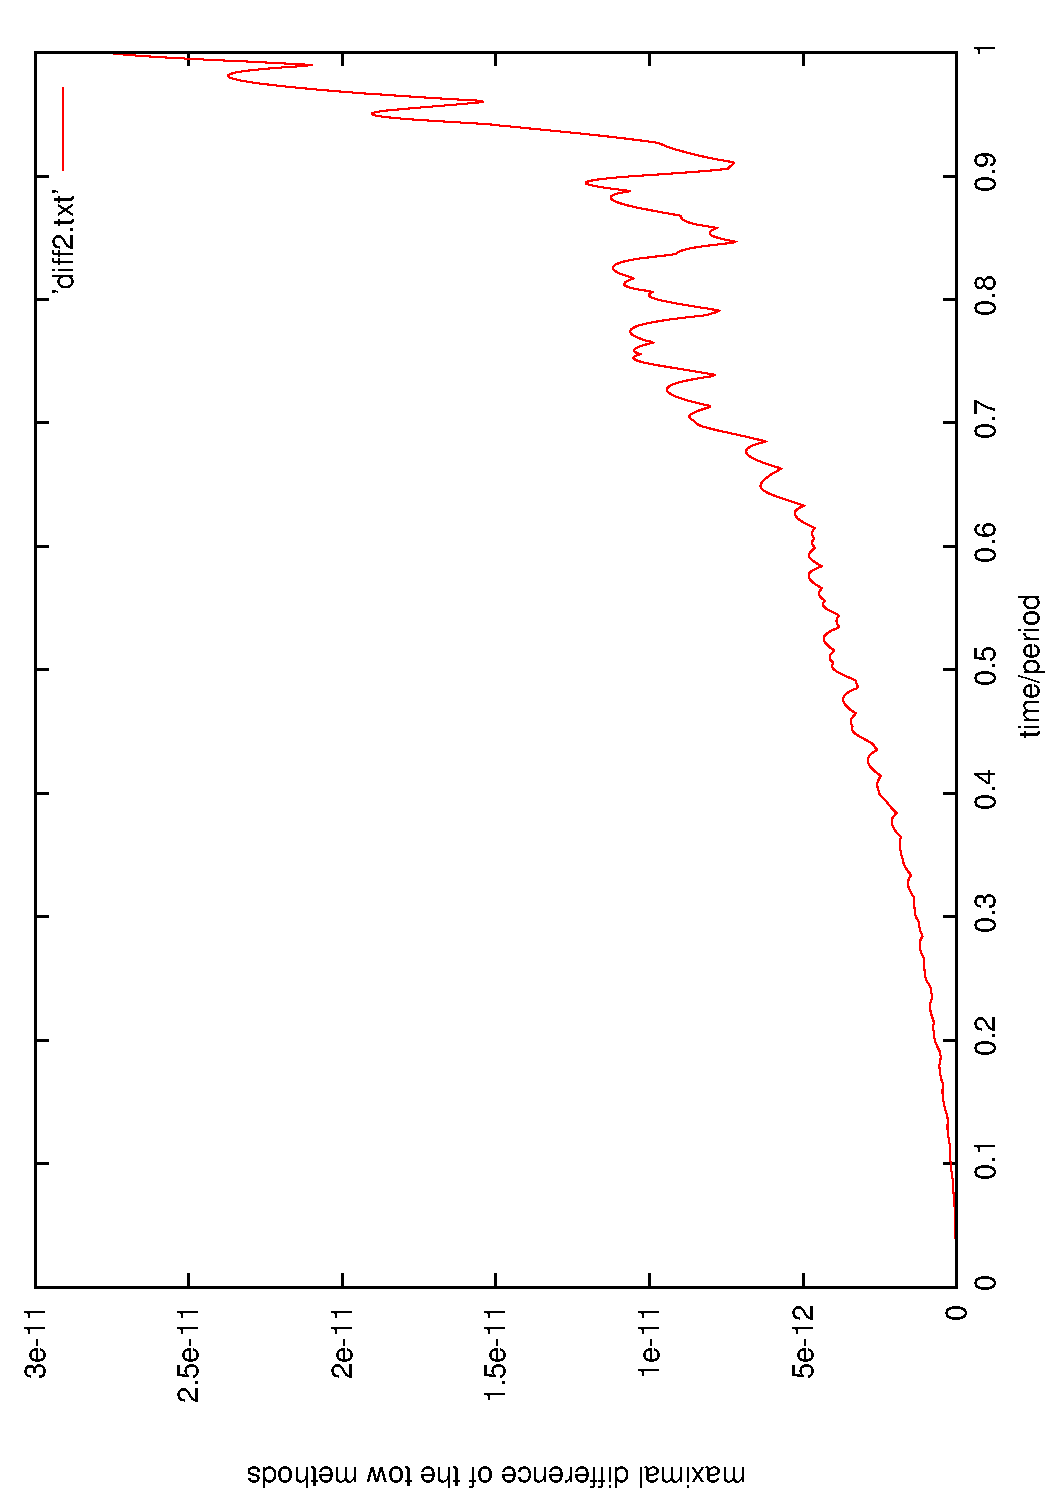
\includegraphics[angle=-90,width=0.5\textwidth]{diff-eps-converted-to.pdf}
 \caption{the maximal difference of the fourier modes for one period along the periodic orbit
  $T10.25$.}
 \label{fig:xiong_sdmfft_dif}
\end{figure}

\clearpage

%%%----------------------------------------------------------------------------
\subsection{Chebyshev Differential Matrix }
\begin{description}
\item[2013-09-25 Xiong]
\end{description}

We know that the Discrete Fourier transform is a good tool to interpolate a periodic function,
 but what if the function is not periodic? Suppose there is a function $f(x)$ defined in $[-1,1]$.
 We make $f(x)$ to be periodic in
 $(-\infty, \infty)$ with period $2$ just by extending its value in $[-1,1]$ in two directions, and
 then use Fourier Differential Matrix to calculate its derivative in $[-1,1]$. However,
 this is a bad idea
 because extended function is not smooth now at points $x=\dots, -3,-1,1,3,\dots,$, which will result
 in the lose of accuracy of Fourier Differential Matrix.

 Another choice is to use polynomials $p(x)=a_{0}+a_{1}x+\dots+a_{N}x^{N}$ to interpolate $f(x)$
 in $[-1,1]$. Suppose there are $N+1$ sample points $x_{j},\quad j=0,1,2 \dots ,N$, then
 the error associated with polynomial interpolation is:
 \[
  err(x)=f(x)-p(x)=\frac{f^{N+1}(\varepsilon)}{(N+1)!}\Pi_{i=0}^{N}(x-x_{i})
 \]
 So a good interpolant will try to minimize $\Pi_{i=0}^{N}(x-x_{i})$.
 Now we turn to the question of how to choose sample points.

 \begin{enumerate}
  \item Equispaced interpolant: $x_{i}=\frac{2j}{N}-1,\quad j=0,1,\dots, N $. This is the choice
  emergeing in my mind the first time I think of interpolant, but it is not a good candidate for
  sample points, because the oscillations near the boundery will get worse
  when $N$ increases, which is called Runge phenomenon. At the same time, this method is less accurate
  than Chebyshev interpolant.
  For example, choosing $x=(N-1)/N$ and $N=30$ we have
  \[
   |\Pi_{i=0}^{N}(x-x_{i})|= \frac{(2N-1)!!}{N^{N+1}}\approx 4.7\times 10^{-6}
  \]


  \item Chebyshev interpolant: $x_{j}=\cos(\frac{j\pi}{N}), \quad j=0,1,2,\dots N$.
  These points are the maximal or minimal points of $N_{th}$ order Chebyshev polynomial:
  $T_{N}(x)=\cos(N\cos^{-1}(x))$, so they are (except $x_0$ and $x_N$)
  the zeros of $\frac{dT_{N}(x)}{dx}=NU_{N-1}=N\sin N\theta/\sin\theta$, where $U_{N-1}$
  is the second type Chebyshev polynomial and $x=\cos\theta$.
  \begin{align*}
   \prod_{i=0}^{N}(x-x_{i}) &=(x-x_0)(x-x_N)\prod_{i=1}^{N-1}(x-x_{i})\\
   &=\frac{1}{2^{N-1}}\frac{\sin N\theta}{\sin\theta}(x-1)(x+1)\\
   &=\frac{-1}{2^{N-1}}\sin N\theta \sin\theta
  \end{align*}

  The coefficient $1/2^{N-1}$ comes from the following fact: the highest order
  in $T_{N}(x)$ is $2^{N-1}x^{N}$ because of the recursive relation
  $T_{N}(x)=2xT_{N-1}(x)-T_{N-2}(x)$ and initial conditions $T_{0}=0,\quad T_{1}=x$;
  meanwhile, from $\frac{dT_{N}(x)}{dx}=N\sin N\theta/\sin\theta$ we know the highest order
  coefficient in  $\sin N\theta/\sin\theta$ is also $2^{N-1}$. Therefore, coefficient
  $1/2^{N-1}$ is required to rewirte $\prod_{i=0}^{N}(x-x_{i})$.

  \[
   |\prod_{i=0}^{N}(x-x_{i})|=\frac{1}{2^{N}} |\sin N\theta \sin\theta| \leq \frac{1}{2^{N}}
  \]

  When $N=30$,  $\frac{1}{2^{N-1}}\approx 1.8\times 10^{-9}$. Now we can see that Chebyshev interpolant
  is superior to equispaced interpolant. If larger $N$ is choosen, the accuracy of Chebyshev interpolant
  is far better than that of equispaced interpolant. More importantly,
  Chebyshev interpolant circumvents the
  Runge phenomenon.


\end{enumerate}

  We now need to write down the specific form of polynomial that interpolate the discrete set
  $u_{j}=u(x_j),j=0,1,\dots,N$ at points $x_{j}=\cos(\frac{j\pi}{N})$, which is trivial:
  \begin{equation}
   P(x)=\sum_{j=0}^{N}p_{j}(x)u_{j}=\sum_{j=0}^{N}u_{j}\frac{\prod_{k\neq j}(x-x_{k})}{\prod_{k\neq j}(x_{j}-x_{k})}
  \end{equation}

  Obviously, $p_{j}(x_{i})=\delta_{ij}$. Define $a_{j}=\prod_{k\neq j}(x_{j}-x_{k})$; thus we have:
  \[
   \frac{p_{i}(x)}{x-x_{j}}=\frac{a_j}{a_i} \frac{p_{j}(x)}{x-x_{i}}
  \]

  In order to calculate $dP(x)/dx$, we can use
  identity $\frac{d(\ln p_{j}(x))}{dx}=\sum_{k\neq j}(x-x_{k})^{-1}$. Therefore,
  \begin{align*}
   \frac{dP(x)}{dx} &= \sum_{j=0}^{N}p_{j}(x)\sum_{k\neq j}\frac{1}{x-x_{k}}u_{j}\\
   &=  \sum_{j=0,j\neq i}^{N}p_{j}(x)\sum_{k\neq j}\frac{1}{x-x_{k}}u_{j}+
   p_{i}(x)\sum_{k\neq i}\frac{1}{x-x_{k}}u_{i}\\
   &=  \sum_{j=0,j\neq i}^{N}[p_{j}(x)\sum_{k\neq j,k\neq i}\frac{1}{x-x_{k}}u_{j}+
   p_{j}(x)\frac{1}{x-x_{i}}u_{j}]+p_{i}(x)\sum_{k\neq i}\frac{1}{x-x_{k}}u_{i}\\
  \end{align*}

  Evaluated at point $x_{i}$, it becomes
  \begin{align*}
   & \frac{dP(x_{i})}{dx}\\
   & =\sum_{j=0,j\neq i}^{N} p_{j}(x_{i})\frac{1}{x-x_{i}}u_{j}
   +p_{i}(x_{i})\sum_{k\neq i}\frac{1}{x_{i}-x_{k}}u_{i}\\
   & =\sum_{j=0,j\neq i}^{N}\frac{a_i}{a_j}\frac{p_{i}(x_{i})}{x_{i}-x_{k}}u_{j}
   +p_{i}(x_{i})\sum_{k\neq i}\frac{1}{x_{i}-x_{k}}u_{i}\\
   & =\sum_{j=0,j\neq i}^{N}\frac{a_i}{a_j}\frac{1}{x_{i}-x_{k}}u_{j}
   +\sum_{k\neq i}\frac{1}{x_{i}-x_{k}}u_{i}\\
  \end{align*}

  Therefore, we can write down the Chebyshev Differential matrix:
  \[
   D_{i,j}=
   \begin{cases}
    \frac{a_{i}}{a_{j}(x_{i}-x_{j})} & (i\neq j)\\
    \sum_{k\neq i}\frac{1}{x_{i}-x_{k}} & (i=j)
   \end{cases}
  \]

  The next step is to determine $a_{i}/a_{j}$ and $\sum_{k\neq i}\frac{1}{x_{i}-x_{k}}$. Define
  \[A(x)=\prod_{i=0}^{N}(x-x_{i})
  \,.
  \] From previous discussion, we know
  \[
   A(x)=\frac{-1}{2^{N-1}}\sin N\theta\sin\theta
  \]
  where $\theta=\cos^{-1}(x)$.

  \textbf{Claim 1}: $$A^{'}(x_{j})=a_{j}=\prod_{k\neq j}(x_{j}-x_{k})$$
  proof: $$A^{'}(x)=\sum_{j=0}^{N}\prod_{k\neq j}(x-x_{k})\Rightarrow
  A^{'}(x_{j})=\prod_{k\neq j}(x_{j}-x_{k}) $$

 \textbf{Claim 2}: $$\frac{A^{''}(x_{j})}{2A^{'}(x_{j})}=\sum_{k\neq i}\frac{1}{x_{i}-x_{k}}$$
 proof:
 \begin{align*}
 & A^{''}(x)=\sum_{i=0}^{N}\sum_{j\neq i}\prod_{k\neq i, k\neq j}2(x-x_{k})\\
 \Rightarrow & A^{''}(x_{j})=2\sum_{i\neq j}\prod_{k\neq i, k\neq j}(x_{j}-x_{k})\\
 \Rightarrow & \frac{A^{''}(x_{j})}{2A^{'}(x_{j})}=
 \frac{2\sum_{i\neq j}\prod_{k\neq i, k\neq j}(x_{j}-x_{k})}{2\prod_{k\neq j}(x_{j}-x_{k})}
 =\sum_{k\neq i}\frac{1}{x_{i}-x_{k}}
  \end{align*}

 The next step is easy: just evaluate $A^{'}(x_j)$ and $A^{''}(x_j)$. You can turn to chain rule
 to make life easier: $dA(x)/dx=dA(\theta)/d\theta \cdot d\theta/dx$. Meanwhile,
 $A^{'}(x)$ and $A^{''}(x)$ are singular at points $x=\pm 1$, so you can take
 $\lim_{x\to \pm 1}$ to get the values.

 In summary,
  \[
   -2^{N-1}A^{'}(x_j)=
   \begin{cases}
    2N & (j=0)\\
    2(-1)^{N}N & (j=N)\\
    (-1)^{j}N & (j\neq 0,N)
   \end{cases}
  \]

  \[
   -2^{N-1}A^{''}(x_j)=
   \begin{cases}
    \frac{4N^3+2N}{3} & (j=0)\\
    (-1)^{N}\frac{4N^3+2N}{3}  & (j=N)\\
    \frac{(-1)^{N+1}Nx_{j}}{1-x_{j}^{2}} & (j\neq 0,N)
   \end{cases}
  \]

  Eventually, we can write down the explicit formula for Chebyshev Differential matrix:
  \[
   D_{ij}=\frac{c_i}{c_j}\frac{(-1)^(i+j)}{x_{i}-x_{j}} \quad i\neq j
  \]
  \[
   D_{jj}=\frac{-x_{j}}{2(1-x^{2}_{j})} \quad j\neq 0,N
  \]
  \[
   D_{00}= \frac{2N^2+1}{6} ,\quad D_{NN}= -\frac{2N^2+1}{6}
  \]


\section{Exponential time-differencing with embedded
          Runge–Kutta adaptive step control}
\label{sect:RKadapt}

Exponential time-differencing (ETD) scheme has been widely used to solve semilinear
problem of type
\begin{equation}
  \label{eq:sl}
  y'(t) = f(t, u) = \mathcal{L} y + \mathcal{N}(t, y)
\end{equation}
Often the nonlinear part is non-stiff compared with the linear part.
ETD method integrates the linear part explicitly and approximates the nonlinear part
by expansion series. More specifically,
ETD Runge-Kutta methods (ETDRK)\rf{cox02jcomp} and
Integrating factor (IF)\rf{Lawson67} are the most two
popular methods used to solve \refeq{eq:sl}. Recently, exponential Rosenbrock
method\rf{Luan2014}
is raised to solve systems with both stiff linear and stiff nonlinear part.
Here we focus on ETDRK method. Coefficients of Butcher table
in ETDRK are exponential matrix
functions like $e^{h\mathcal{L}}$, which need to be recalculated whenever
the time step is varied. Therefore, time adaptive scheme is not performance
advantageous especially for large full $\mathcal{L}$, and thus literature
on time adaptive scheme is sparse. However, for certain physical systems like
\cGLe, which exhibit intermittent burst, time adaptive scheme is
preferable compared with constant time step scheme for its ability slow down
the integration for the burst part. Recently, P. Whalen \etal\rf{Whalen2015} formed
two time-adaptive ETDRK methods (ETD34 and ETD35) and numerical tests clearly shows
that time adaptive scheme is superior to constant time stepping for integrating the
nonlinear schr\"{o}dinger equation.

\paragraph{Background}
Exact integration of \refeq{eq:sl} can be performed
using matrix exponentials
\begin{equation}
  \label{eq:SLexact}
  y(t_{n+1}) = e^{h\mathcal{L}}y(t_n) + \int_0^h e^{(h-\tau)\mathcal{L}}
  \mathcal{N}(t_n+\tau, y(t_n+\tau)) d\tau
\end{equation}
Here $h = t_{n+1} - t_n$ is the time step.
Inspired by this formula, we let $z=e^{-t\mathcal{L}}y$, and get velocity of $z$
\begin{equation}
  \label{eq:slz}
  z'(t) = e^{-t\mathcal{L}}\mathcal{N}(t, e^{t\mathcal{L}}z)
\end{equation}
So you can see linear part is integrated explicitly and only nonlinear part is left.
Substitute \refeq{eq:slz} into a general s-stage explicit RK scheme
\begin{align*}
  Y_i & = u_n + h\sum_{j=1}^{i-1} a_{ij}f(t_n + c_jh, Y_j) \\
  y_{n+1} & = y_n + h\sum_{i=1}^{s} b_i f(t_n + c_ih, Y_i)
\end{align*}
then we obtain
\begin{align*}
  Y_i & = e^{hc_i\mathcal{L}}u_n + h\sum_{j=1}^{i-1} a_{ij}e^{h\alpha_{ij}\mathcal{L}}
        \mathcal{N}(t_n + c_jh, Y_j) \\
  y_{n+1} & = e^{h\mathcal{L}}y_n + h\sum_{i=1}^{s} b_i e^{h\beta_i\mathcal{L}}
            \mathcal{N}(t_n + c_ih, Y_i)
\end{align*}
where $\beta_i=1-c_i$ and $\alpha_{ij}=c_i-c_j$. We can see that the Butcher table
has changed from $(a_{ij}, b_i)$ to
$(a_{ij}e^{h\alpha_{ij}\mathcal{L}}, b_i e^{h\beta_i\mathcal{L}})$. More generally, these
coefficients can be functions of $h\mathcal{L}$:
\begin{align}
  Y_i & = e^{hc_i\mathcal{L}}u_n + h\sum_{j=1}^{i-1} a_{ij}(h\mathcal{L})
        \mathcal{N}(t_n + c_jh, Y_j) \label{eq:ETDRKa}\\
  y_{n+1} & = e^{h\mathcal{L}}y_n + h\sum_{i=1}^{s} b_i(h\mathcal{L})
            \mathcal{N}(t_n + c_ih, Y_i) \label{eq:ETDRKb}
\end{align}
Our goal is to find suitable functions for $a_{ij}(h\mathcal{L})$,
$b_i(h\mathcal{L})$ to obtain desired order of local truncation error.
Such functions could have arbitrary form, and usually we need to expand
them in series
\[
a_{ij}(h\mathcal{L}) = \sum_{k} a_{ijk}\varphi_{k}(h\mathcal{L})\,,\quad
b_{i}(h\mathcal{L}) = \sum_{k} b_{ik}\varphi_{k}(h\mathcal{L})
\]
and truncate at certain order. The choice or expansion
bases $\varphi_k$ directly determines the quality of such truncation.
To see how to choose $\varphi_k$, we turn to \refeq{eq:SLexact} and
take Taylor expansion of nonlinear part with
$\mathcal{N}(t_n+\tau, y(t_n+\tau))$ approximated by $\mathcal{N}(t_n+\tau, y(t_n))$.
\begin{align*}
  \label{eq:nlTaylor}
  y(t_{n+1}) & = e^{h\mathcal{L}}y(t_n) + \int_0^h e^{(h-\tau)\mathcal{L}}
               \mathcal{N}(t_n+\tau, y(t_n+\tau)) d\tau \\
             & \simeq e^{h\mathcal{L}}y(t_n) + \int_0^1 e^{(1-\theta)h\mathcal{L}}
               \mathcal{N}(t_n+ \theta h, y(t_n)) d\theta \\
             & = e^{h\mathcal{L}}y(t_n) + \sum_{r=0}^{\infty} h^r \mathcal{N}^{(r)}
               \int_0^1 \frac{e^{(1-\theta)h\mathcal{L}}\theta^r}{r!} d\theta \\
             & = e^{h\mathcal{L}}y(t_n) + \sum_{r=0}^{\infty} h^r \mathcal{N}^{(r)}
               \varphi_{r+1}(h\mathcal{L})\\
\end{align*}
with
\begin{equation}
  \label{eq:nlphi}
  \varphi_j(z) =  \int_0^1 e^{(1-\theta)z}\frac{\theta^{j-1}}{(j-1)!} d\theta
\end{equation}
We set $\varphi_0(z)=e^{z}$, and there is a recursion relation
$\varphi_{k+1}(z) = \frac{\varphi_{k}(z)-1/k!}{z}$. The first few bases are
\[
  \varphi_1(z)= \frac{e^z-1}{z}\,,\quad
  \varphi_2(z)= \frac{e^z-z-1}{z^2}\,,\quad
  \varphi_3(z)= \frac{e^z-z^2/2-z-1}{z^3}
\]
ETDRK methods documented in literature almost at most reach the 3rd base, since
higher order base are expensive to evaluate numerically.

\paragraph{Nonstiff order condition} Same as the Rouge Kutta scheme, Taylor series
of \refeq{eq:SLexact} is compared with that of \refeq{eq:ETDRKb} truncated at
a certain order to get the corresponding order condition.
This is a tedious work when trying to derive high order differentials of
$\mathcal{N}(t, u(t))$.
Analogous to B-series and rooted trees\rf{Lambert1991},
H. Berland \etal\rf{Berland05} use a bicolored tree to take account of both
linear and nonlinear parts in higher order derivatives.
Order condition derived in this approach
is called \emph{nonstiff order condition} because
such conditions are not aware of stiffness of the problem.
See Theorem 2.1 and table 2 in\rf{Berland05} for the exact formulae.

\paragraph{Stiff order condition} The nonstiff order condition has a problem when
Linear part $\mathcal{L}$ is very stiff since truncation of series
$e^{h\mathcal{L}} = I + h\mathcal{L} + \frac{1}{2}(h\mathcal{L})^2 + \cdots $ to a
certain order does not make any sense if $\mathcal{L}$ has a large norm.
Based on the exact local truncation analysis, V. T. Luan \etal\rf{LuOs13} recover
the set of order equation which include the nonstiff order condition a set
of additional order conditions, called \emph{stiff order condition}. See table 5.1
in\rf{LuOs13}. For a numerical scheme which only satisfies a lower stiff order
condition than the nonstiff order condition, it may suffer order reduction
for stiff equations. Therefore, a good numerical scheme should try to reach
the same nonstiff and stiff order conditions.

\paragraph{ETDRK4 and Krogstad scheme}
ETDRK4 was organically developed by Cox and Matthews\rf{cox02jcomp} and later was
improved by Kassam and Trefethen\rf{ks05com} to cope with integration of
bases \refeq{eq:nlphi} by contour integral. Krogstad\rf{Krogstad2005}
is credited with
improving Cox and Matthews’ method by slightly changing its Butcher table
resulting in slightly better convergence and stability. He called it ETDRK4-B
in\rf{Krogstad2005}. \refTab{eq:etdrk4} and \reftab{eq:krogstad}
are the Butcher table for these two schemes respectivly.
\begin{equation}
  \label{eq:etdrk4}
  \begin{tabular}{c | c c c c}
    0 & & & & \\
    $\frac{1}{2}$  & $\frac{1}{2}\varphi_{1, 2}$ &&&\\
    $\frac{1}{2}$ & 0 & $\frac{1}{2}\varphi_{1, 3}$ &&\\
    1 & $\frac{1}{2}\varphi_{1,3}(\varphi_{0,3}-1)$ & 0 & $\varphi_{1,3}$ & \\
    \hline
      & $\varphi_{1}-3\varphi_{2}+4\varphi_{3}$ & $2\varphi_{2}-4\varphi_{3}$
          & $2\varphi_{2}-4\varphi_{3}$ & $4\varphi_{3}-\varphi_{2}$ \\
  \end{tabular}
\end{equation}
\begin{equation}
  \label{eq:krogstad}
  \begin{tabular}{c | c c c c}
    0 & & & & \\
    $\frac{1}{2}$  & $\frac{1}{2}\varphi_{1, 2}$ &&&\\
    $\frac{1}{2}$ & $\frac{1}{2}\varphi_{1, 3} -\varphi_{2, 3}$ & $\varphi_{2, 3}$ &&\\
    1 & $\varphi_{1,4}-2\varphi_{2,4}$ & 0 & $2\varphi_{2,4}$ & \\
    \hline
      & $\varphi_{1}-3\varphi_{2}+4\varphi_{3}$ & $2\varphi_{2}-4\varphi_{3}$
          & $2\varphi_{2}-4\varphi_{3}$ & $4\varphi_{3}-\varphi_{2}$ \\
  \end{tabular}
\end{equation}
Here, $\varphi_i = \varphi_i(h\mathcal{L})$ is the base functions \refeq{eq:nlphi}
and
$\varphi_{i,j}=\varphi_i(c_jh\mathcal{L})$. The notation used here follows that
in\rf{Hochbruck05}. You can check both the nonstiff and stiff order conditions for
these two schemes, and it turns out that both have nonstiff order 4. ETDRK4 has
stiff order 2 and Krogstad scheme has stiff order 3. So This explains why
Krogstad scheme has better performance than ETDRK4 for stiff problems.

\paragraph{Embedded Rouge Kutta for adaptive step control}
Dormand Prince method\rf{Dormand86} and Runge Kutta Fehlberg method
are
both frequently used Runge Kutta method with adaptive step control.
They use an embedded scheme to estimate the local truncation error, on which
time step changes are based. Here we follow\rf{Whalen2015} to formulate two
adaptive time step method based on ETDRK4 and Krogstad scheme.
\begin{equation}
  \label{eq:etdrk4Adapt}
  \begin{tabular}{c | c c c c c}
    0 & & & & &\\
    $\frac{1}{2}$  & $\frac{1}{2}\varphi_{1, 2}$ &&&&\\
    $\frac{1}{2}$ & 0 & $\frac{1}{2}\varphi_{1, 3}$ &&&\\
    1 & $\frac{1}{2}\varphi_{1,3}(\varphi_{0,3}-1)$ & 0 & $\varphi_{1,3}$ & &\\
    1 & $\varphi_{1}-3\varphi_{2}+4\varphi_{3}$ & $2\varphi_{2}-4\varphi_{3}$
          & $2\varphi_{2}-4\varphi_{3}$ & $4\varphi_{3}-\varphi_{2}$ & \\
    \hline
    $b_i$  & $\varphi_{1}-3\varphi_{2}+4\varphi_{3}$ & $2\varphi_{2}-4\varphi_{3}$
          & $2\varphi_{2}-4\varphi_{3}$ & $4\varphi_{3}-\varphi_{2}$  & 0\\
   $\bar{b}_i$  & $\varphi_{1}-3\varphi_{2}+4\varphi_{3}$ & $2\varphi_{2}-4\varphi_{3}$
          & $2\varphi_{2}-4\varphi_{3}$ & 0 & $4\varphi_{3}-\varphi_{2}$ \\
  \end{tabular}
\end{equation}
\begin{equation}
  \label{eq:krogstadAdapt}
  \begin{tabular}{c | c c c c c}
    0 & & & & & \\
    $\frac{1}{2}$  & $\frac{1}{2}\varphi_{1, 2}$ &&&&\\
    $\frac{1}{2}$ & $\frac{1}{2}\varphi_{1, 3} -\varphi_{2, 3}$ & $\varphi_{2, 3}$ &&&\\
    1 & $\varphi_{1,4}-2\varphi_{2,4}$ & 0 & $2\varphi_{2,4}$ & & \\
    1 & $\varphi_{1}-3\varphi_{2}+4\varphi_{3}$ & $2\varphi_{2}-4\varphi_{3}$
          & $2\varphi_{2}-4\varphi_{3}$ & $4\varphi_{3}-\varphi_{2}$ & \\
    \hline
    $b_i$ & $\varphi_{1}-3\varphi_{2}+4\varphi_{3}$ & $2\varphi_{2}-4\varphi_{3}$
          & $2\varphi_{2}-4\varphi_{3}$ & $4\varphi_{3}-\varphi_{2}$ & 0 \\
    $\bar{b}_i$  & $\varphi_{1}-3\varphi_{2}+4\varphi_{3}$ & $2\varphi_{2}-4\varphi_{3}$
          & $2\varphi_{2}-4\varphi_{3}$ & 0 & $4\varphi_{3}-\varphi_{2}$ \\
  \end{tabular}
\end{equation}

In both \reftab{eq:etdrk4Adapt} and \reftab{eq:krogstadAdapt},
a nonstiff 3th order and stiff 2nd order method is
embeded. The estimated local truncation error is
\begin{equation}
  \label{eq:LTE}
  R_{n+1} = \bar{y}_{n+1} - y_{n+1} = b_4\left[\mathcal{N}(t_n+h, Y_5)-
    \mathcal{N}(t_n+h, Y_4)\right]
\end{equation}
These two adaptive schemes only introduce one additional evaluation of function
$\mathcal{N}(t, y)$.

Let the local error tolerance is $\epsilon ||y_{n}||_2$, then the time step
adaption rule is
\[
  h_{new} = vh\left(\frac{\epsilon ||y_{n}||_2}{||R_{n+1}||_2} \right)^{1/4}
\]
Here $v=0.9$ is a safe factor. For performance consideration, only the difference
between $h_{new}$ and $h$ is large enough, we update time step and refill the
Butcher table. See\rf{Whalen2015} for more detailed treatment on adapting time
step.

\paragraph{Numerical experiments in \cqcGLe}

\begin{figure}[h]
  \centering
  \begin{minipage}{.25\textwidth}
    \centering \small{\texttt{(a)}}
    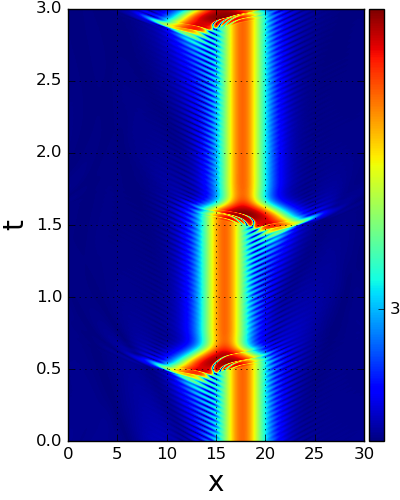
\includegraphics[width=\textwidth]{cglETDphase1}
  \end{minipage}
  \begin{minipage}{.25\textwidth}
    \centering \small{\texttt{(b)}}
    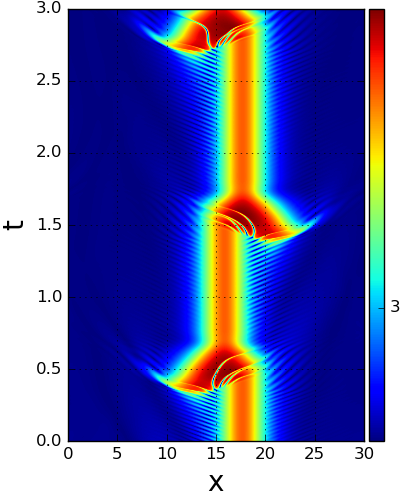
\includegraphics[width=\textwidth]{cglETDphase2}
  \end{minipage}%
  \begin{minipage}{.25\textwidth}
    \centering \small{\texttt{(c)}}
    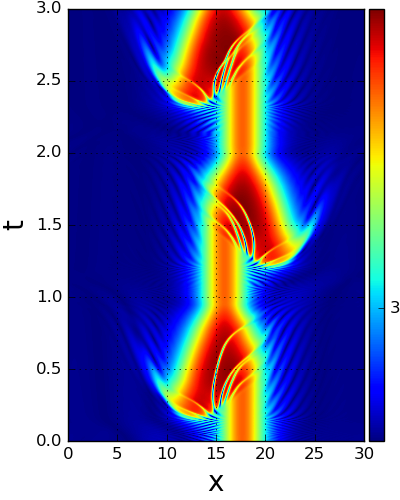
\includegraphics[width=\textwidth]{cglETDphase3}
  \end{minipage}
  \caption{ Soliton explosion profiles by Krogstad scheme :
    (a) Constant time step  $h=10^{-3}$.
    (b) Adaptive time step in static frame.
    (c) Adaptive time step in traveling frame.
  }
  \label{fig:cglETDphase}
\end{figure}

\begin{figure}[h]
  \centering
  \begin{minipage}{.32\textwidth}
    \centering \small{\texttt{(a)}}
    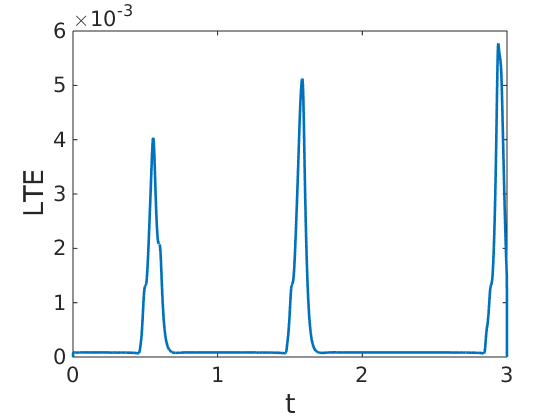
\includegraphics[width=\textwidth]{cglETDLTE1}
  \end{minipage}
  \begin{minipage}{.32\textwidth}
    \centering \small{\texttt{(b)}}
    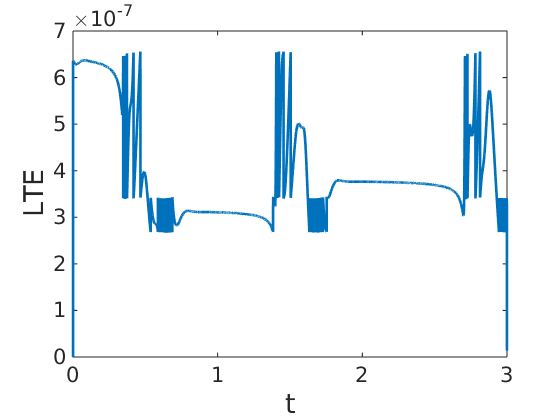
\includegraphics[width=\textwidth]{cglETDLTE2}
  \end{minipage}%
  \begin{minipage}{.32\textwidth}
    \centering \small{\texttt{(c)}}
    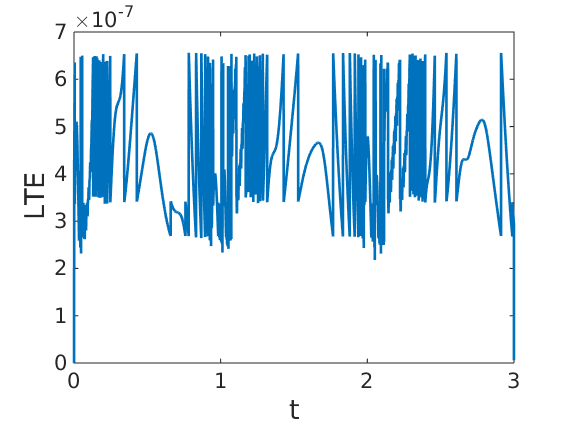
\includegraphics[width=\textwidth]{cglETDLTE3}
  \end{minipage}
  \caption{ Estimated local truncation error by Krogstad scheme :
    (a) Constant time step $h=10^{-3}$.
    (b) Adaptive time step in static frame.
    (c) Adaptive time step in traveling frame.
  }
  \label{fig:cglETDLTE}
\end{figure}

\begin{figure}[h]
  \centering
  \begin{minipage}{.4\textwidth}
    \centering \small{\texttt{(a)}}
    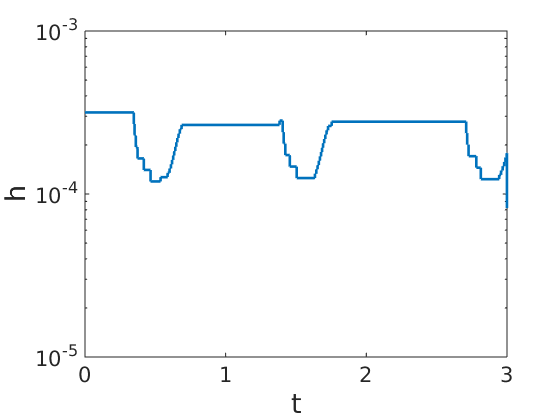
\includegraphics[width=\textwidth]{cglETDh2}
  \end{minipage}
  \begin{minipage}{.4\textwidth}
    \centering \small{\texttt{(b)}}
    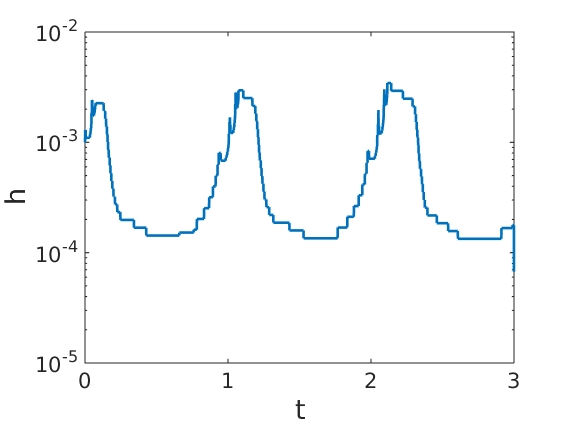
\includegraphics[width=\textwidth]{cglETDh3}
  \end{minipage}%
  \caption{ Time step used during integration by Krogstad scheme :
    (a) Adaptive time step in static frame.
    (b) Adaptive time step in traveling frame.
  }
  \label{fig:cglETDh}
\end{figure}

\begin{table}[h]
  \centering
  \begin{tabular}{c  c c  c c}
    & \multicolumn{2}{c}{ETDRK4} & \multicolumn{2}{c}{Krogstad} \\
    \hline
    &  TA & TATF & TA & TATF \\
    NReject &  51 & 86 & 51 & 108 \\
    NevaCoe &  87 & 141 & 87 & 178 \\
    Ns & 12532 & 4653 & 12581 &  4544 \\
    \hline
  \end{tabular}
  \begin{tabular}{l l }
    & \\
    TA  &  Time adaptive scheme \\
    TATF &  Time adaptive in traveling \\
         & frame scheme \\
    NRject &  number of time the calculated \\
           &  new state is rejected due to large \\
           &  estimated local truncation error  \\
    NevaCoe &  number of time to recalculate Butcher table \\
    Ns & number of integration steps \\
  \end{tabular}
  \caption{
    Compassion between ETDRK4 and Krogstad.
  }
  \label{tab:ETDKrog}
\end{table}

As an experiment, we test the performance of the time step adaptive ETDRK4 and
Krogstad in one dimensional \cqcGLe.
In a certain range of parameters, this system exhibits intermittent
explosion. So the dynamics of this system has two different time scales :
every slow movement around a relative equilibrium  and
every fast burst when the soliton explodes. We anticipate the time step adaptive
ETDRK4 and Krogstad can slow down at the explosion part and accelerate at the
slow part.

In the experiments, we set the integration time period to be $[0, 3]$ and the
relative error tolerance $\epsilon=10^{-6}$. The constant time step schemes use
time step $h=10^{-3}$. All tests use the same initial condition.

\refFig{fig:cglETDphase} (a)(b) show the evolution of $|A|$ using
constant time step and adaptive time step Krogstad method respectively.
During the integration period, three explosion instances are observed. The
explosion parts in (b) are stretched a little bit compared with (a) because the
time adaptive scheme slows down during explosion parts.
\refFig{fig:cglETDLTE} (a)(b) are the corresponding estimated local truncation
error during the same period. Without local error control, the constant time step
Krogstad has bad performance for the explosion part, during which local truncation
error reaches as large as $6\times 10^{-3}$. While local truncation
error is controlled under $10^{-6}$ for time step adaptive scheme.

However, as shown in \reffig{fig:cglETDh}(a) the time step adaptive Krogstad
method still uses every small time step ($\sim 3\times 10^{-4}$)
even for the slow motion part. In fact, the stiffness actually comes from fast phase
rotation of complex field $A$. Until now, we are only interested in the magnitude
of field $A$ and turn a blind eye to its phase. However, orbits of this system in
the state space is circulating around a relative equilibrium of the form
\[
  A_0(t, x) = A_0(x)e^{i\omega_0 t}
  \,
\]
with phase rotating velocity $\omega_0 =176.675049$ a very large number. Thus dynamics
close to this relative equilibrium will have similar large phase rotation.
Therefore, we integrate the system in a traveling frame by setting
\[
  A(x, t) = \tilde{A}(x, t)e^{i\omega_0 t}
\]
The dynamics of $\tilde{A}(x, t)$ is shown in \reffig{fig:cglETDphase}(c). The
corresponding local truncation error and time steps are shown in
\reffig{fig:cglETDLTE} and \reffig{fig:cglETDh} respectively. We can see that
time step used in this traveling frame is almost one order larger that that in the
static frame for the slow motion part. But for the explosion part, both use time
step $\sim 10^{-4}$.

Time step adaptive ETDRK4 is also tested and the result is compared with
Krogstad method in \reftab{tab:ETDKrog}. The difference between these two
methods are minimal. Since ETDRK4 has more empty locations in its Butcher
table, evaluation of Butcher table is more efficient in ETDRK4 than Krogstad.
So, in practice, we prefer to use adaptive ETDRK4 to integrate \cqcGLe.
\refTab{tab:ETDKrog} also shows that integration in the traveling frame is
much more efficient than in the static frame.

\paragraph{Some notes}
For record purpose, I list the coefficients of Butcher table in
ETDRK4 and Krogstad for easy implementation.
\begin{itemize}
\item ETDRK4
  \[
    E = e^{hL}\,,\quad 
    E_2 = e^{hL/2}\,,\quad
    a_{21} = \frac{e^{hL/2}-1}{L}
  \]
  \begin{align*}
    b_1 & = h^{-2}L^{-3}[-4-hL+e^{hL}(4-3hL+(hL)^2)] \\
    b_2 = b_3 & = 2h^{-2}L^{-3}[2+hL+e^{hL}(-2+hL)] \\
    b_4 & = h^{-2}L^{-3}[-4-3hL-(hL)^2+e^{hL}(4-hL)] \\
  \end{align*}
  \begin{align*}
    U_1 & = u_n \\
    U_2 & = E_2 u_n + a_{21} \mathcal{N}(t_n, u_n) \\
    U_3 & = E_2 u_n + a_{21} \mathcal{N}(t_n+\frac{h}{2}, U_2) \\
    U_4 & = E_2 U_2 + a_{21} (2\mathcal{N}(t_n+\frac{h}{2}, U_3)-
          \mathcal{N}(t_n, u_n) )\\
    U_5 & = E u_n + b_{1} \mathcal{N}(t_n, u_n)
          +b_2[\mathcal{N}(t_n+\frac{h}{2}, U_2) + 
          \mathcal{N}(t_n+\frac{h}{2}, U_3)]
          +b_4 \mathcal{N}(t_n+h, U_4) )\\
    u_{n+1} & = U_5
  \end{align*}
  A trick is used in $U_4$.

\item Krogstad scheme.
  $E$, $E_2$, $a_{21}$, $b_1$, $b_2$ $b_3$ and $b_4$ are the same as 
  ETDRK4.
  Other coefficients are 
  \[
    a_{31} =  h^{-1}L^{-2}[4+hL+e^{hL/2}(hL-4)]\,,\quad 
    a_{32} =  2h^{-1}L^{-2}[-2-hL+2e^{hL/2}]
  \]
  \[
    a_{41} =  h^{-1}L^{-2}[2+hL+e^{hL}(hL-2)]\,,\quad 
    a_{43} =  2h^{-1}L^{-2}[-1-hL+e^{hL}]
  \]
  \begin{align*}
    U_1 & = u_n \\
    U_2 & = E_2 u_n + a_{21} \mathcal{N}(t_n, u_n) \\
    U_3 & = E_2 u_n + a_{31} \mathcal{N}(t_n, u_n) +
          a_{32} \mathcal{N}(t_n+\frac{h}{2}, U_2) \\
    U_4 & = E_2 u_n + a_{41}\mathcal{N}(t_n, u_n) 
          + a_{43}\mathcal{N}(t_n+\frac{h}{2}, U_3) \\
    U_5 & = E u_n + b_{1} \mathcal{N}(t_n, u_n)
          +b_2[\mathcal{N}(t_n+\frac{h}{2}, U_2) + 
          \mathcal{N}(t_n+\frac{h}{2}, U_3)]
          +b_4 \mathcal{N}(t_n+h, U_4) )\\
    u_{n+1} & = U_5
  \end{align*}
\end{itemize}

%%%%%%%%%%    end of the differential matrix part     %%%%%%%%%%%%%%%%%%%%%%%%%%%%

    \newpage
\section{Study notes of (periodic) Krylov-Schur algorithm}
\label{sect:KrylovSchur}

For a large eigenvalue problem or Floquet analysis in a high dimensional dynamical system,
only a subset of its eigenvalues is of interest. To achieve this goal, Sorensen 
\etc\rf{Sorensen1992} proposed
implicit restarted Arnoldi method with polynomial filter. This method restricts the dimension
of Krylov subspace and substantially saves the storage space; at the same time, 
this algorithm is implemented in ARPACK and is free to use. 
However, its deflating strategy is complicated\rf{Lehoucq1996}. Later on,
G. W. Stewart\rf{Stewart02} relaxed the Hessenberg form of Arnoldi iteration, and proposed the 
Krylov decomposition. Moreover, he proved that this new algorithm is equivalent to
Sorensen's algorithm but much easier to understand and implement. It requires
Schur decomposition, so it is named Krylov-Schur algorithm.

Later, D. Kressner\rf{Kressner2006} 
extends Krylov-Schur algorithm to solve product eigenvalue 
problem\rf{Wat2005, Wat07}, which
is called periodic Krylov-schur algorithm.  

A few remarks about the implementation:
\begin{itemize}
\item The case that the initial vector is within an invariant subspace of the 
  matrix concerned. Suppose the dimension of this subspace is $k$, then the 
  usual Arnoldi process terminates after $k$ iterations because the $k$-th
  diagonal element of Hessenberg matrix is very small. However, for our 
  purpose, I think it is fine to continue no matter how small this element 
  is because our goal is to obtain a set of orthonormal vectors. The double
  orthonormalizaiton trick guarantees that the $(k+1)$-th vector is perpendicular
  to the first $k$ vectors.
\end{itemize}

    \newpage
\ifsvnmulti
 \svnkwsave{$RepoFile: xiong/blog/KSe.tex $}
 \svnidlong {$HeadURL: svn://zero.physics.gatech.edu/siminos/xiong/blog/KSe.tex $}
 {$LastChangedDate: 2017-02-15 00:24:45 -0500 (Wed, 15 Feb 2017) $}
 {$LastChangedRevision: 5559 $} {$LastChangedBy: xiong $}
 \svnid{$Id: KSe.tex 5559 2017-02-15 05:24:45Z xiong $}
\fi

\section{\KSe}
\label{sect:KSe}

\PC{2013-03-19 Predrag copied this from \refref{SCD07}, to set up
the conventions for the \KSe\ calculations.}
%
In the formulation
adopted here, the time evolution of the `flame front velocity'
$u=u(x,t)$ on a periodic domain $u(x,t) = u(x+L,t)$ is given by
\beq
  u_t = F(u) = -{\textstyle\frac{1}{2}}(u^2)_x-u_{xx}-u_{xxxx}
    \,,\qquad   x \in [-L/2,L/2]
    \,.
\ee{ks}
Here $t \geq 0$ is the time, and $x$ is the spatial coordinate.
The subscripts $x$ and $t$ denote partial derivatives with respect to
$x$ and $t$. In what follows
we shall state results of all calculations either in units of the
`dimensionless system size' $\tildeL$, or the system size $L = 2 \pi
\tildeL$. All numerical results presented in this report
are for $\tildeL=22/2\pi \simeq 3.5014$.
Spatial periodicity $u(x,t)=u(x+L,t)$
makes it convenient to work in the Fourier space,
\beq
  u(x,t)=\sum_{k=-\infty}^{+\infty} a_k (t) e^{ i k x /\tildeL }
\,,
\ee{eq:ksexp}
with the $1$-dimensional PDE \refeq{ks}
replaced by an infinite set of
ODEs for the complex Fourier coefficients $a_k(t)$:
\beq
\dot{a}_k= \pVeloc_k(a)
     = ( q_k^2 - q_k^4 )\, a_k
    - i \frac{q_k}{2} \sum_{m=-\infty}^{+\infty} a_m a_{k-m}
\,,
\ee{expan}
where $q_k = k/\tildeL$.
Since $u(x,t)$ is real, $a_k=a_{-k}^\ast$, and we can replace the
sum by a $k > 0$ sum.


\begin{description}

\item[2013-06-27 Predrag to \XD] Read the other chapters in this blog,
    study the relevant \KS\ papers\rf{SCD07,Christiansen97}.

\item[2013-07-03 \XD] Here is my first blog post: A question about the
    \KS\ equation. It seems that there are many versions of KS
    equation, and some of them are totally different. The one you used
    in \refref{SCD07}, ``On the {\statesp} geometry of the KS flow in a
    periodic domain'' is \beq
 u_t=-\frac{1}{2}(u^2)_x-u_{xx}-u_{xxxx}
\ee{XD-KSeSCD07}
However, the
equation in \refref{KNSks90}, ``Back in the saddle again: a computer
assisted study of the KS equation'' is:
\beq
 u_t+4\bigtriangleup^2 u
    +\alpha (\bigtriangleup u +\frac{1}{2}(\bigtriangledown u)^2)=0
\ee{XD-KSeSCD07a}
The first order term is different.

\item[2013-07-04 Predrag] That is always annoying when one reads
KS literature - I asked that Evangelos include various transformations
in his thesis, but I cannot find that text, only this:
``The parameter $\alpha$ of \refrefs{KNSks90,ksgreene88} is
related to the system size by $\tildeL=\sqrt{\alpha/4}$.''

In Evangelos
\HREF{../blog/blog.pdf} {blog} we write

``
The {1\dmn} \KSe\ as given in \refrefs{KurTsu75,siv} is (up to overall scaling
factors):
\beq
    y_t=-y_x^2/2-y_{xxxx}-y_{xx}
\,,\qquad       x \in [0,L]
\,,
    \label{eq:KSeOR}
\eeq
with periodic boundary conditions in the $[0,L]$ interval. The form used
here
\beq
    u_t=uu_x-u_{xxxx}-u_{xx}
\,.
    \label{eq:KSeAP}
\eeq
is obtained from \refeq{eq:KSeOR} by differentiating with respect to $x$
and setting \PCedit{$u=-y_x$}.
In study of {1\dmn} \KS\ \eqva\ $x$ in \refrefs{LanThesis,ksgreene88}
is interpreted as ``time", so $y$ is a height of a front,
and $y_x$ its ``velocity".
In the literature  both forms of the equation are
referred to as the \KSe.
''

In Evangelos blog I rescued the text that he did not use in his thesis,
copied below.
Let us know whether this resolves your quandary,
and please do remember to include this in your project
report, so it is available to future students (I should really
include it into an appendix to ChaosBook...)            \toCB

\item[2007-01-20 Evangelos]
Notes on Greene and Kim\rf{ksgreene88}. A copy is in ChaosBook.org/library,
\HREF{http://chaosbook.org/library/index.html}{click here}.

\noindent\textbf{\Eqva\ according to Greene and Kim:}
%
The form of \KSe\ studied by Greene and Kim\rf{ksgreene88} is
\beq
    y_t=-4y_{xxxx}-\alpha\left(y_{xx}+\frac{1}{2}y_x^2
            -\frac{1}{4\pi}\int_0^{2\pi}y_x^2\ dx\right)
\,,\qquad       x \in [0,2\pi]
\,,
    \label{eq:KSeGreeneKim}
\eeq
with  periodic boundary condition on the interval $[0,2\pi]$.
Mean elastic energy density of a spatial profile $y(x,t)$ is defined by
\beq
    E=\frac{1}{2\pi}\int_0^{2\pi}y_x^2\, dx\,.
    \label{KSenergy}
\eeq
% \ES{This definition does not only apply to equilibria. Greene and
% Kim also study the transfer of energy between modes
% in non-stationary trajectories.}.
Taking the derivative of \refeq{eq:KSeGreeneKim}
with respect to $x$ and substituting $y_x=-u$ leads to
\[
    u_t=4u_{xxxx}+\alpha\left(u_{xx}-uu_x\right)
\,.
\]
Rescaling
\beq
    \tilde{x}=\frac{\sqrt{\alpha}}{2} x
\,,\qquad
    \tilde{t}=\frac{\alpha^2}{4} t
\,,\qquad
    \tilde{u}=\frac{2}{\sqrt{\alpha}} u
    \label{eq:GKscale}
\eeq
brings the Greene-Kim equation to the form \refeq{eq:KSeAP} used here.
The dimensionless system size $\tildeL=L/2\pi$ is related to
the Greene-Kim parameter
through $\tildeL=\sqrt{\alpha}/2$.
The system size $L=22$ studied here corresponds to $\alpha=49.0395$.

The ``kinetic energy'' reads in our units:
\PC{shouldn't there be a prefactor $\frac{1}{2}$?}
\beq
    \tilde{E}=\frac{1}{L}\int_0^{L}\tilde{u}^2\, d\tilde{x}\,.
\eeq
Integrating \refeq{ks} in $[0,L]$ we get $c=\tilde{E}$,
since the terms involving $u_x$ and $u_{xxx}$ vanish due to periodicity.
From the scalings \refeq{eq:GKscale} we have $\tilde{E}=\frac{4}{\alpha}E$.


\item[2013-07-03 \XD] In \refref{SCD07} you point out KS equation is
    Galilean invariant: if $u(x,t)$ is a solution, then $u(x-ct)-c$ is
    also a solution. but I am confused, because when I substitute it
    into the equation I get a minus sign. If I change the form to be
    $u(x-ct)+c$, then it is OK.

\item[2013-07-04 Predrag] Thanks for noticing this - you are correct, see
2nd paragraph of Section ChaosBook {\em 26.1.1 Scaling and symmetries.}
(all ChaosBook section and eq.~numbers refer to the stable
\HREF{http://chaosbook.org/version14/pdf.shtml} {version 14} of Dec.
31 2012). The error has propagated from Evangelos
\HREF{http://chaosbook.org/projects/theses.html} {thesis},
{\em section 5.1.2 Symmetries of Kuramoto-Sivashinsky system} to the article.

Embarrassing, but too small an error to change the arXiv version of \refref{SCD07}
(though Evangelos could fix it in his thesis)...

Now I note that the ChaosBook {\em Exercise
26.1.
Galilean invariance of the Kuramoto-Sivashinsky equation} is also in error.
As you are checking the KS papers anyhow, you would help me a lot if you also
checked {\em Chapter 27 Turbulence?} as you went along - that chapter is still
only a draft, has been very hard to write up concisely...
Please correct \refexer{exer-GalInv}, write up the solution
(I'll transfer it back to ChaosBook).                   \toCB
\\{\bf [2013-07-12 \XD] done.}

\item[2013-07-11 \XD] Yesterday I talked with Prof. Predrag and I was
    sceptical about the $1/2$ coefficient in the Fourier transform
    \refeq{expan} of the \KS\ equation \refeq{XD-KSeSCD07}.
\[
 u_t=-\frac{1}{2}(u^2)_x-u_{xx}-u_{xxxx}
 \,.
\]
We perform Fourier transform:
\[
 u(x,t)=\sum_{k=-\infty}^{+\infty} a_{k}(t)e^{ikx/\tilde{L}}
\]
For the nonlinear term $-\frac{1}{2}(u^2)_x$, we get
$-i\frac{q_k}{2}\sum_{m=-\infty}^{+\infty} a_{m}a_{k-m}$,
where $q_k=k/\tilde{L}$. It has the form of
convolution, which comes from one property of Fourier transform.
Now I try to write it down in detail:
\begin{align*}
 -\frac{1}{2}(u^2)_x &=-uu_x \\
 &=-\sum_{m=-\infty}^{+\infty} a_{m}(t)e^{imx/\tilde{L}}
 \sum_{n=-\infty}^{+\infty} \frac{in}{\tilde{L}} a_{n}(t)e^{inx/\tilde{L}}\\
 &=-\sum_{m=-\infty}^{+\infty}\sum_{n=-\infty}^{+\infty} iq_{n} a_{m}(t)e^{iq_{m}x}a_{n}(t)e^{iq_{n}x}\\
 &=-\frac{i}{2}\sum_{m=-\infty}^{+\infty}\sum_{n=-\infty}^{+\infty}
 (q_{n}+q_m) a_{m}(t)e^{iq_{m}x}a_{n}(t)e^{iq_{n}x}\\
 &=-\frac{i}{2}\sum_{m=-\infty}^{+\infty}\sum_{n=-\infty}^{+\infty} q_{n+m} a_{m}(t)a_{n}(t)e^{i(q_{n}+q_m)x}
\end{align*}
If we take out the coefficient of term $e^{iq_{k}x}$, it will give
$-i\frac{q_k}{2}\sum_{m=-\infty}^{+\infty} a_{m}a_{k-m}$, thus the
Fourier transform \refeq{expan} is correct.

\item[2013-07-12 \XD] Wrote up solution to \refexer{exer-GalInv}, {\em
    Galilean invariance of the \KSe.}

\item[2013-07-12 Predrag] Created the research level \refexer{exer-locGalInv},
{\em Local Galilean invariance of \KS.}

\item[2013-06-27 Predrag  to \XD] A discussion of stiffness in
    integrating PDEs can be found
    \HREF{http://www.pvv.ntnu.no/~berland/talks/berland05expintro.pdf}
    {here}. \HREF{http://www.math.ntnu.no/num/expint/} {Here} is Matlab
    package for testing 47 (!) schemes.

Study the methods described in
\HREF{http://www.cns.gatech.edu/~predrag/papers/SCD07.pdf}
{Appendix A} of \refref{SCD07}.
%The authors have lots of experience and they went to the
%    trouble of explaining the best methods they know, so why not read
%    them and implement them?

The plot of what you get for $L=22$
Lyapunov spectrum should confirm the published results (see
{\bf [2009-09-13 Ruslan]} on \refpage{sect:LyapKS},
\reffig{fig:lyapSpecCLG}, \reffig{fig:lyapSpec1},
\reffig{fig:lyapSpec}, and \reftab{tab:ks22shad}) and the
figure\PC{which one? Always state the number} in Kazumasa \etal\
paper\rf{TaGiCh11} (read it
\HREF{http://chaosbook.org/library/KoSa11.pdf} {here}).

\item[2013-06-27 Ruslan]
You can use the method developed by Cox and
Matthews\rf{cox02jcomp} and improved by Kassam and
Trefethen\rf{ks05com}, where the linear part is integrated exactly.
My Matlab code {\tt ksfmetd2.m} is based on this method and it is
stable and reasonably accurate with time step as large as 0.25.  It
also solves variational problem, so can be used to calculate Lyapunov
exponents.  See {\tt ksfmlyap.m} in {\tt siminos/matlab/ruslan/},
read {\tt 00ReadMe.txt}.  If you want to compute Lyapunov exponents
using the standard GS procedure, the relevant code is in {\tt
ksdupo.m} in the same folder (look for the cell "\%\% Compute
Lyapunov exponents of KS (using ksfmlyap and GS)").

\item[2013-06-27 Predrag]
Ruslan uses the same \KSe\ convention as Kassam and
Trefethen\refrefs{ks05com}. I have saved the Trefethen Matlab code
\HREF{http://chaosbook.org/extras/Trefethen/kursiv.m} {here}. Perhaps
you want to c++ it, see how it runs for you, or run it in Matlab and
compare with your code. There might be something else useful on
\HREF{http://chaosbook.org/extras/}{ChaosBook.org/extras} homepage,
for example the simulations by the spring 2007 GaTech chaos class.
You can search the blog for 'Trefethen' for other discussions
(Kazumasa has reservations about the Trefethen\rf{ks05com} algorithm,
but Ruslan is OK with it).
Siminos has other codes, if needed, on a different repository.

\item[2013-01-21 Evangelos] The \KS\ data you need is in \\
\texttt{siminos/matlab/ruslan/kse22orbits.mat},
\\
in a structure called \texttt{eq}.
Eigenvalues are in the field eq.eig and right
eigenvectors are in the field eq.evec. [e.g. eq(k).evec(:,1) is the
eigenvector which corresponds to the first eigenvalue eq(k).eig(1) of
the k'th equilibrium]. However, I have not used the data for a long
time so, it would be better if Ruslan verifies how the Fourier modes
are stored (I think that the numbers in a column vector correspond to
real and imaginary part of the Fourier modes
\[
 (a_1,\, b_1,\, a_2,\, b_2,\, \ldots a_N,\, b_N)
\]
and thus here there are $31+1$ complex Fourier modes (the zero'th mode
is not included)).

In order to get the left eigenvectors you will need to compute the
{\stabmat}.

If you run into problems or have questions please email me so that we
can arrange to talk through Skype.


\item[2013-06-27 Ruslan] To compute {\stabmat} in Matlab, use
\\
\texttt{siminos/matlab/ruslan/ksfm.m}:
\\ {\tt [f, df] = ksfm(0,eq(1).a,22.0)},
\\where {\tt df} will be the {\stabmat} of $EQ_1$.

The idea of the method is described in \refref{SCD07} Appendix A and
B.  The Jacobian matrix is calculated from (B.1) which uses solutions
of (A.4) and (A.6).  Matlab code {\tt ksfmetd2.m} solves (A.4) and
(A.6) simultaneously.  The Jacobian matrix is output in {\tt da}.
You don't need anything else.


\item[2013-07-23 \XD] I don't understand one point of Appendix A in
    paper \rf{SCD07}. After Fourier transform,
\[
 u(x,t)=\sum_{k=0}^{N} a_{k}(t)e^{ikx/\tilde{L}}
\]
we have relation $a_{N-k}^{~}=a_{k}^{*}$ and set $a_0=0$ due to Galilean
invariance, but why can we also set $a_{N/2}=0$ ?
\\
{\bf [2013-07-24 Predrag]} The first relation is due to the reality of
\( u(x,t) \). I suspect that the second one is due to the periodicity
\( u(x,t) = u(x+L,t) \). Let me know if I am wrong?

\item[2013-07-24  \XD] Why both $a_{N/2}=0$ and $a_0=0$? I think
    $a_{N/2}=0$ comes from Galilean invariance of \KS\ equation; while
    we set $a_0=0$ just for the convenience to perform the discrete
    Fourier transform. It is not one component of the Fourier spectrum
    because we are using discrete Fourier transform to truncate the
    nonlinear term in continuous Fourier transform. Am I right?

\item[2013-07-30 Evangelos to \XD] $\dot{a}_0=0$ by Galilean invariance
    and thus $a_0$ is constant. We \emph{choose} this constant to be
    zero so that the mean value of our solutions is zero. Otherwise you
    would get ``drifting solutions.'' $a_{N/2}=0$ is the DFT analog of
    $a_k=a^*_{-k}$, which holds in general for Fourier series of real
    data. (This is discussed in my thesis.)

\item[2013-07-24  \XD] the initial condition of $T_{10.25}$ in
\\*
\texttt{siminos/matlab/ruslan/ks22f90h25t100.mat}
was used in my code. Hoping to get a
periodic graph, I failed. After scrutinizing my code carefully,
I could not find an error, so I suspected that maybe some variables
defined in Ruslan's code were differently
from mine.

I compared my code with \texttt{siminos/matlab/ruslan/ksfmetd2.m},
there is a major difference at the form of the coefficient before the nonlinear term.
Ruslan used \texttt{g = 0.5i*k*N}, but I prefer to \texttt{g=-0.5i*k}.
Such a difference results from the slightly different use of discrete Fourier transform
and the conjugacy of $a_k$, which is \PCedit{$a_{N-k}=a^{*}_k$}.

If we prefer the discrete Fourier transform defined in the Appendix A of
\refref{SCD07},
\[
 u(x,t)=F_N^{-1}[a]_n=\frac{1}{N}\sum_{k=0}^{N-1} a_{k}(t)e^{iq_{k}x_{n}}
\,,
\]
\KS\ equation will be transformed to
\[
 \dot{a_k}=(q_{k}^2-q_k^4)a_k-i\frac{q_k}{2}F_{n}[(F_N^{-1}[a])^2]_k
\,.
\]

Note that the nonlinear term is
\[
-i\frac{q_k}{2}F_{n}[(F_N^{-1}[a])^2]_k=-i\frac{q_k}{2}\frac{1}{N}\sum_{m=-\infty}^{+\infty}a_{m}a_{k-m}
\,.
\]
I think maybe Ruslan hopes the transformed equation is consistent with the form
\[
 \dot{a_k}=(q_{k}^2-q_k^4)a_k-i\frac{q_k}{2}\sum_{m=-\infty}^{+\infty}a_{m}a_{k-m}
\,,
\]
so he keeps the coefficient before the nonlinear term by $N$ times larger.

The sign of the coefficient is defined by whether you treat $\mathbf{a}(t_0)$ as inital condition or
$\mathbf{a}^{*}(t_0)$.


In conclusion, if I insist on my style, I should transform the initial condition $\mathbf{a}(t_0)$
for $T_{10.25}$  to $N\mathbf{a}*(t_0)$, but I think it is better to follow predecessors' style.

\item[2013-07-30 Evangelos to Xiong]
It seems everyone of us uses a different normalization of FFT and sometimes this leads to
confusion. I would suggest that you follow Ruslan's conventions so that you do not need to transform
his data. Also, if you write C++ or Fortran code, I recommend using the excellent FFTW library.




\end{description}

% 2013-11-20 Predrag removed this: \input{../xiong/doc/blog/xcomm.tex}

\subsection{The dimension of \KSe }

\KSe is usually transformed into Fourier space for its benefit of
transforming higher derivatives in the {\statesp} into polynomial terms
in Fourier space. In numerical implementation, we turn to  \xDft  with
truncation number $N$ :  $u_{0}, u_{1}, \cdots, u_{N-1}$.

\[
	\begin{bmatrix}
	a_{0} \\
	a_{1} \\
	\vdots \\
	a_{N-1}
	\end{bmatrix}
	=
	\begin{bmatrix}
	\omega^{0*0} & \omega^{0*1} & \cdots & \omega^{0*(N-1)}\\
	\omega^{1*0} & \omega^{1*1} & \cdots & \omega^{1*(N-1)}\\
	\vdots & \vdots &\ddots & \vdots \\
	\omega^{(N-1)*0} & \omega^{(N-1)*1} & \cdots & \omega^{(N-1)*(N-1)}
	\end{bmatrix}	
	\begin{bmatrix}
	u_{0} \\
	u_{1} \\
	\vdots \\
	u_{N-1}
	\end{bmatrix}
\]

These Fourier modes satisfy $a^{*}_k=a_{N-k} (\mod N)$, which means that
$a_{N/2}$ and $a_{0}$ are both real. This linear transform conserves the freedom
of this system
\[
v_{0},	v_{1},\cdots , v_{N-1} \Rightarrow a_{0}, a_{R,1}, a_{I,1}, \cdots ,
a_{R,N/2-1}, a_{I,N/2-1}, a_{N/2}
\]

Since Floquet multipliers are metric invariant, we can turn to the
Fourier space to calculate the Flouqet multipliers of periodic orbits. At
the same time, the {\cLvs} in the {\statesp} $e^{(i)}_{u}$  and those in
the Fourier space $e^{(i)}_{a}$  satisfy
\[
	e^{(i)}_{a}=M_{i,j}e^{(j)}_{u}
\]

where $M$ is the transforming matrix from $v_{0},	v_{1},\cdots , v_{N-1}$ to \\
$a_{0}, a_{R,1}, a_{I,1}, \cdots , a_{R,N/2-1}, a_{I,N/2-1}, a_{N/2} $.


The flow in the Fourier space is governed by
\begin{equation}
 \dot{a_k}=(q_{k}^2-q_k^4)a_k-i\frac{q_k}{2}F_{N}[(F_N^{-1}[a])^2]_k
 \,.
\end{equation}

In \KS\ system, we set $a_{0}=0$ due to Galilean invariance  and also set  $a_{N/2}=0$ because
$a_{N/2}$ is decoupled from other modes ($q_{N/2} = 0$ for symmetry of the definition of
discrete Fourier Transform), so it decreases rapidly to zero. Therefore, the freedom
of this system is now $N-2$. The flow equation in the tangent space is governed by
\begin{equation}
 \dot{b_k}=(q_{k}^2-q_k^4)b_k-iq_{k} F_{N}[(F_N^{-1}[a])\otimes (F_N^{-1}[b])]_k
 \label{eq:xkstang}
\end{equation}

The initial jacobian matrix in the  \\
$[a_{0}, a_{R,1}, a_{I,1}, \cdots , a_{R,N/2-1}, a_{I,N/2-1}, a_{N/2} ]$ space is  Identity matrix,
which is mapped to $B(0)$ as the initial condition
for equation \ref{eq:xkstang}.
\[B(0)=
\begin{bmatrix}
	0 & 0 & 0 & 0 & \cdots  \\
	1 & 1i & 0 & 0 & \cdots  \\
	0 & 0 & 1 & 1i & \cdots  \\
	\vdots & \vdots  & \vdots &\vdots &\ddots{} \\
	0 & 0 & 1 & -1i & \cdots  \\
	1 & -1i & 0 & 0 & \cdots
\end{bmatrix}
\]

%=======================================================%
\paragraph{Equilibria of \KS\ system at L=22}

I used damped Newton-Raphson method described in \rf{Crofts07thesis} to locate equilibria of
\KSe\ at L=22 and truncation number $N=32$, and I find three equilibria and
calculate their stability exponents. The result is
consistent with that in \refref{SCD07}.

 \begin{figure}[h]
 \centering
 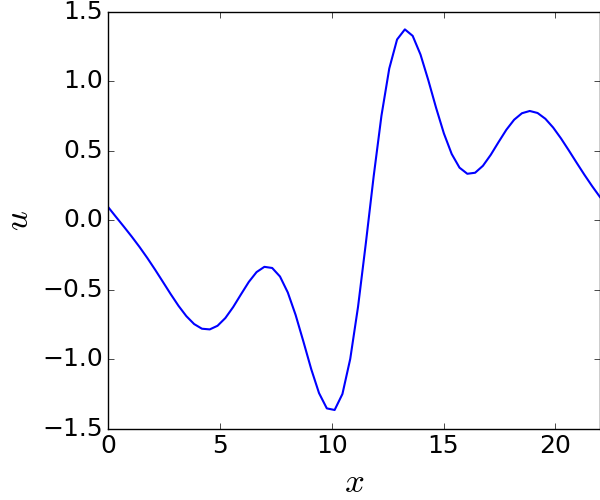
\includegraphics[width=0.3\textwidth]{ksEq1}
 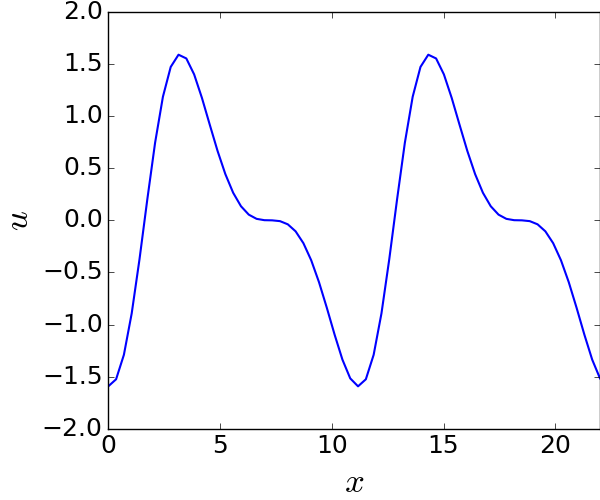
\includegraphics[width=0.3\textwidth]{ksEq2}
 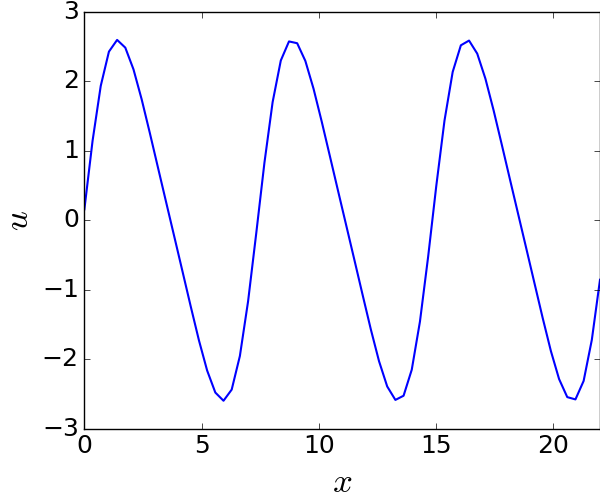
\includegraphics[width=0.3\textwidth]{ksEq3}
 \caption{\Eqva\ solutions in the configuration space.}
 \label{fig:xequi1}
\end{figure}

\begin{figure}[h]
 \centering
 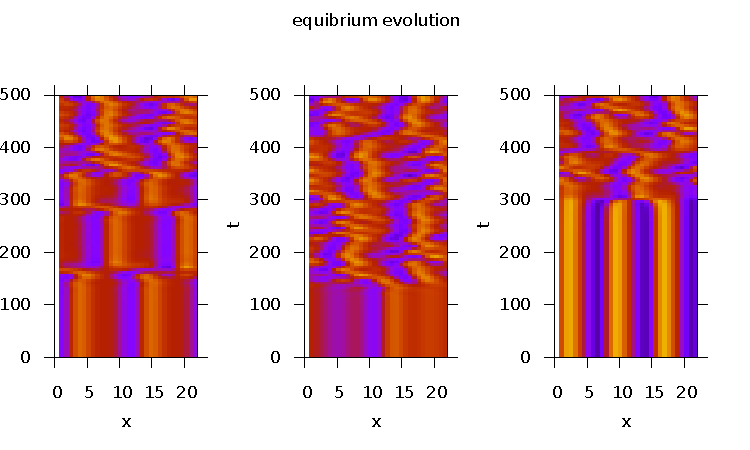
\includegraphics[width=0.8\textwidth]{equi2.pdf}
 \caption{Evolution starting from these \eqva.}
 \label{fig:xequi2}
\end{figure}

\refFig{fig:xequi1} is not as smooth as that in \rf{SCD07} and the magnitude of the waves has different
scales and phases. The underlining reason for the difference is that
 we have slightly different definitions of \xDft and  these equilibria exhibit  translational invariance.

 \refFig{fig:xequi2} is the evolution of these equilibria. Since they are unstable, the states turn to be
 chaotic after about 100 time units for the first two equilibria, while the third one stays about 300 time units
 before collapse.



 For equilibria, the {\stabmat} is constant $A(x_{eq})$; so is the jacobian matrix
 $J^{t}(x_{eq})=\exp(A(x_{eq})t)$.
 Therefore, the stability exponents are just the eigenvalues of $A(x_{eq})$ and the {\cLvs}
 are just the eigenvectors of $A(x_{eq})$.  The stability exponents  are exactly the same with those documented in
 \rf{SCD07} , here I only post my result for $E_{3}$ equilibrium.
 \\
   0.09335 + 0.00000i \\
   0.09334 + 0.00000i \\
  -0.00000 + 0.00000i  \\
  -0.41277 + 0.00000i\\
  -0.61075 + 0.37587i\\
  -0.61075 - 0.37587i \\
  -0.61075 + 0.37588i \\
  -0.61075 - 0.37588i \\
  -1.66413 + 0.00000i \\
  -1.66413 + 0.00000i \\

The other two sets of exponents are saved in \\
\texttt{/siminos/xiong/matlab/equilibria}.


\paragraph{Relative equilibria}
Relative equilibrium is defined as $u(x,t) = u(x-ct)$,
which means $f_{k}(a) = v_{k}(a) +icq_{k}a_{k}$. The second term  $cq_{1}t(a)$
is a vector in group tangent direction
in $\mathbb{U}(1)$ space. In order to implement Newton's method, we need to get the
explicit form of $f'_{k}$:
\begin{equation}
  \begin{bmatrix}
    A + cq_{1}\mathbf{T} & q_1  t(a) \\
    t(a) & 0
  \end{bmatrix}
  \cdot
  \begin{bmatrix}
    \Delta b_1 \\
    \Delta c_1 \\
    \vdots \\
    \Delta c_{N/2-1}
  \end{bmatrix}
  =
  \begin{bmatrix}
    f_{1,R} \\
    f_{1,I} \\
    \vdots \\
    f_{N/2-1,I}\\
  \end{bmatrix}
  \,.
  \label{eq:relativeeq}
\end{equation}
$\mathbf{T}$ is the generator of SO(2), and $A$ is the {\stabmat}
in the full state space. The last row in \ref{eq:relativeeq} comes from the
constraint $t(a)\cdot \Delta a = 0$. For \KS\ system with $L=22$, only two
relative equilibria
are found. Note that equation \ref{eq:relativeeq} is also capable
detecting equilibria ($c = 0$). Relative equilibrium is moving on the
group orbit $x(t)=g(-ctq_1)x(0)$, and the relation of {\stabmat}
at different points on this group orbit is simple.
$A(x)\delta x = \delta v(x)$ and $A(gx)\delta(gx)=\delta v(gx)$ infer
$A(gx)g\delta x = g\delta v(x)$, which is $A(gx)g=gA(x)$, so the
eigenvectors of $A$
at point $x$ and $g(-ctq_1)x$ are related by group transformation
$g(-ctq_1)$; however, this vector is not covariant along the group
trajectory. since $J^{\delta t}v=(1+A\delta t)v = (1+\lambda\delta t) v$,
which is not in the same direction as
$g(\delta \theta)v = v+\delta\theta \mathbf{T}v$. According to
Chaosbook, The correct {\stabmat} in this case is
$A+cq_1\mathbf{T}$.

The reasoning behind is every simple. Let's consider a general case:
$x(t)=g(ct)x(0)$. The Jacobian is decomposed as
\[
J^{\zeit} = J^{\Delta t} (x_n) J^{\Delta t} (x_{n-1})\cdots  J^{\Delta t} (x_1)
\,,
\]
where $\Delta t = t/n$ and $x_{k}=g[c(k-1)\Delta t] x_1$. Since
$J(gx)=gJ(x)g^{-1}$, we have
\begin{align*}
J^{\zeit} & = g[c(n-1)\Delta t]J^{\Delta t} (x_1)g^{-1}[c(k-1)\Delta t]
\cdots J^{\Delta t} (x_1) \\
& = [g(-c\Delta t)J^{\Delta t} (x_1)]^{n} \\
& \approx [1 - c\Delta t \mathbf{T} + \Delta t A]^n \\
& \to e^{(-c\mathbf{T}+A)\zeit}
\end{align*}
Here, $\zeit$ denotes the period of the \reqv. Therefore,
$A-c\mathbf{T}$ is the {\stabmat} for relative equilibria.

 %==========================================================%
\subsection{Symmetry of \KSe }
\label{subsect: symkse}

One-dimensional \KSe\  $u_t=-\frac{1}{2}(u^2)_x-u_{xx}-u_{xxxx}\,,x\in [0,L]$ on a
periodic domain ($L=22$) has three different
symmetry:
\begin{itemize}
\item Galilean invariance. if $u(x,t)$ is a solution, then
  $u(x-ct,t)+c$ is also a solution, where c is a constant
  number. These two solutions have different mean velocity
  $\int dx\, u$.
\item Reflection symmetry.  $Ru(x,t)=-u(-x,t)$ is also a solution
  if $u(x,t)$ is a solution.
\item transitional invariance. $\tau_{l/L}u(x,t)=u(x+l,t)$.
\end{itemize}

Numerically, \KSe\
could be transformed into
Fourier space by discrete Fourier transform with truncation
to $N=32$ or $N=64$.
\[
a_{k}(t)=\sum_{n=0}^{N-1}u(x_{n},t)e^{iq_{k}x_{n}},\quad
u(x_{n},t)=\sum_{k=0}^{N-1}a_{k}(t)e^{iq_{k}x_{n}}
\,.
\]
In this way, dynamics in Fourier space is governed by
\[
\dot{a_k}=(q_{k}^2-q_k^4)a_k-i\frac{q_k}{2}F_{N}[(F_N^{-1}[a])^2]_k
\,,
\]
where $q_k = 2\pi k/L$, and the coefficients are complex
$a_{k}=b_{k}+ic_{k}$.


Since $u(x,t)$ is real, $a_{k}(t)=a^{*}_{N-k}(t)$; thus only half of the
Fourier modes are independent. The zero mode $a_{0}$ denotes the
mean velocity of a solution and $\dot{a}_{0}=0$
 enables eliminating Galilean invariance by
setting $a_{0}=0$.
Also after setting $a_{N/2}=0$ \cite{SCD07}, the number of independent variables is $N-2$,
\begin{equation}
\label{eq:fourierspace}
[b_{1},c_{1},b_{2},c_{2},\cdots,b_{N/2-1},c_{N/2-1}]
\,,
\end{equation}
which is the Fourier state space in the discussion that follows.
On the other hand, reflection and translation invariance in
configuration space corresponds to  equivariance of
 \eqref{eq:fourierspace} under group operation
 $R=diag(-1,1,-1,1,\cdots)$ and  $g(l)=diag(r_{1},r_{2},\cdots,r_{N/2-1})$,
where
\[
r_{k}=
\begin{pmatrix}
  \cos(q_{k}l) & \sin(q_{k}l) \\
  -\sin(q_{k}l) & \cos(q_{k}l)
\end{pmatrix}
,\quad k=1,2,\cdots,N/2-1
\,.
\]

 Since periodic orbits of \KS\ system
are time invariant and equivariant under \SOn{2}\ group transformation
 $g(l)$, there should be two marginal exponents which corresponds
to the velocity field $v(x)$ and group tangent $t(x)=\mathbf{T}x$
respectively, where
$\mathbf{T}$ is the generator of \SOn{2}\ rotation:
\[
\mathbf{T}=diag(t_{1},t_{2},\cdots,t_{N/2-1}),\quad
t_{k}=
\begin{pmatrix}
  0 & q_{k} \\
  -q_{k} & 0
\end{pmatrix}
\,.
\]

Especially, for covariant vectors of pre-periodic orbits.
The Jacobian is defined as $J_{p}=RJ^{T_{p}}$, where $T_{p}$ is the prime
period. The two marginal Floquet vectors $v(x)$ and $t(x)$ have
opposite  Floquet multipliers, namely 1 and -1, that is why \ped\ could tell
them and their corresponding Floquet vectors apart. The prof is very
straightforwards.
\begin{align*}
  J_{p}v(x(0))& = RJ^{T_{p}}v(x(0)) \\
  & = Rv(x(t_{p})) =Rv(Rx(0)) \\
  & =R\cdot R v(x(0)) \\
  & =v(x(0))
\end{align*}

\begin{align*}
  J_{p}t(x(0))&= RJ^{T_{p}}t(x(0)) \\
  & = Rt(x(T_{p})) =Rt(Rx(0)) \\
  & = R\mathbf{T}Rx(0) \\
  & = -\mathbf{T}x(0)=t(x(0))\\
\end{align*}

In the last step, we have use the anti-commutation relation
$R\mathbf{T}=-\mathbf{T}R$ which can be verified easily. Therefore,
the velocity field has positive Floquet multiplier 1 and group
tangent has negative Floquet multiplier -1. In table
\ref{tab:FloqExpPPO1}, we can see the third Floquet vector is
the velocity field while the fourth Floquet vector is the group tangent.

%%%%%%%%%%%%%%%%%%%%%%%%%%%%%%%%%%%%%%%%%%%%
\subsection{\On{2}\ factorization of {\Fd} for \KSe }

\KSe\ is invariant under \On{2}\ symmetry, which joins \SOn{2}\ rotations
with $\Dn{1}=\{e,R\}$ reflections. The expected way of writing down the
symmetry reduced trace formula in this case is referring to
the character table of \On{2}, but could we first quotient out
\SOn{2}\ symmetry in the trace formula and then further discuss the
behavior under reflection $R$, like the one-dimensional map
example
invariant under reflection in the Chaosbook ?

The first problem arising in this procedure is the convergence
of \SOn{2}\ reduced trace formula. According to the argument in
Chaosbook,
\begin{align*}
  \sum_{\beta=0,m=0}^{\infty}\frac{1}{s-s_{m,\beta}}
  = & \sum_{m=-\infty}^{\infty}d_{m} \sum_p T_{p}\sum_{r=1}^{\infty}
    \chi_{m}( g_p^r)
{
 e^{r (\beta A_{p}-sT_{p})}
  \over
 {\left|\det\!\left(1-\tilde{M}_{p}^r\right)\right|}
} \\
    = & \sum_{m=-\infty}^{\infty} \sum_p T_{p}\sum_{r=1}^{\infty} e^{-imr\theta_{p}}
{
 e^{r (\beta A_{p}-sT_{p})}
  \over
 {\left|\det\!\left(1-\tilde{M}_{p}^r\right)\right|}
}
\,,
\end{align*}
where $\theta_{p}$ is the group parameter of $g_{p}$ and $m$ is the
index of non-equivalent irreducible representations.
The second identity rises from the fact that the non-equivalent
irreducible representations of \SOn{2}\ are all one-dimensional:
$e^{-im\phi}$. Here,
\[
\sum_{m=-\infty}^{\infty}e^{-imr\theta_{p}}=
\int dx \sum_{m=-\infty}^{\infty}\delta(x-mr)e^{-i\theta_{p} x}
\]
the Fourier transform of a Dirac Comb. I
don't know how to evaluate this formula. On the other hand,
the trace of {\evOper} is defined as
$\mathcal{L}^{t}(y,x)=\int dx \delta(x-f^{t}(x))$, I don't know
why relative periodic orbits will contribute because they
never close.

\begin{description}

\item[2014-04-24 Xiong Ding]
I found the frequently referred to \refref{Creagh91}, ``Semiclassical
trace formulas in the presence of continuous symmetries'' which is
focused one the trace formula for quantum systems. I don't know whether
it deserves reading because it will take me some time to understand it.
Any opinion?

\item[2014-04-27 Predrag] If I credit a paper, you should try to read it
at some point - it is important to read the literature yourself, and blog
your notes here, I might have missed something important when I read it.
You know this from the periodic Schur decomposition. I try to only credit
papers that are actually relevant to our work. Creagh papers are good.
But you are already doing the right stuff to derive the classical trace
formula, so you do not need to read it urgently.

I will not answer your questions above, because from our conversation
today it looks like you have figured out the derivation.

\item[2014-05-02 Xiong Ding] I had a hard time going through the
argument about
\[
{\cal L}_{ba} (y,x) = D(h)_{ba} {\cal L} (y,x)
\]\noindent
as the starting point to understand discrete factorization. For me,
the projection approach is easier to grasp. Projection
operator is defined as
\[
P_\alpha = \frac{d_\alpha}{|G|} \sum_{h\LieEl\in\Group} \chi_\alpha (h) {\bf h}^{-1}
\]
for a discrete symmetry group
$G=\{{ e},{ g}_2,\ldots,{ g}_{|G|}\}$. The orthogonality and completeness
of projection operator
can be easily verified by the orthogonality relation among characters of
irreducible representation. Define $ \cal L_\alpha=P_\alpha \cal L$, then
the trace of {\evOper} $\cal L$ can be decomposed into a sum of
$ \sum_\alpha \tr {\cal L}_\alpha$ because of the completeness of projection
operators.
\Xiong{2014-05-03}{Here the decomposition of trace just relies on the
completeness of projection operators, we haven't used the commutation
relation between {\evOper} and group transform. Am I right?}
So we only need to investigate the projected trace formula:
\begin{align*}
\tr {\cal L}_\alpha & = \frac{d_\alpha}{|G|}\sum_{h \LieEl\in\Group} \chi_\alpha (h)
{\bf h}^{-1} \int_\pS dx \, {\cal L} ( x,x) \\
& =\frac{d_\alpha}{|G|}\sum_{h \LieEl\in\Group} \chi_\alpha (h) {\bf h}^{-1}
\sum_{a \LieEl\in\Group}\int_{\tilde{\pS}} d(a\tilde{x}) \,{\cal L} (a\tilde{x},a\tilde{x})
\\
& =\frac{d_\alpha}{|G|}\sum_{h \LieEl\in\Group} \chi_\alpha (h) {\bf h}^{-1}\,\cdot
|G|\int_{\tilde{\pS}} d(\tilde{x}) \,{\cal L} (\tilde{x},\tilde{x}) \\
& = d_\alpha \sum_{h \LieEl\in\Group} \chi_\alpha (h) \int_{\tilde{\pS}} d\tilde{x} \,
{\cal L} ({\bf h}^{-1} \tilde{x},\tilde{x})
\end{align*}
In the above derivation, we have used the invariance of {\evOper}
under group transform. For a periodic orbit in the fundamental domain
$\tilde{p}$, we follow the standard argument in Chaosbook and get
\[
\int_{\tilde{\pS}} d\tilde{x} \, {\cal L} ({\bf h}^{-1} \tilde{x},\tilde{x}) =
\cl{\tilde{p}} \sum_{r=1}^\infty { e^{r \beta \cdot \Obser_{\tilde{p}}}
\over  | \det \left( {\bf 1}- {\tilde\monodromy}_{\tilde{p}}^{r} \right)
| } \delta_{n,\cl{\tilde{p}} r}\delta_{h,h_{\tilde{p}}^r}
    \,;
\]
so, the {\Fd} is
\bea
F(z) &=& \prod_\alpha F_\alpha (z)^{d_\alpha}
    \continue   %\,\, , \quad \quad
F_\alpha (z) &=&
{\rm exp}  \left( - {
         \sum_{\tilde{p}} \sum_{r=1}^\infty {1 \over r}
 {\chi_\alpha (h_{\tilde{p}}^r)  z^{\cl{\tilde{p}} r}
e^{r \beta \cdot \Obser_{\tilde{p}}}
 % {\phi_p^r}
 \over  | \det \left( {\bf 1}- {\tilde\monodromy}_{\tilde{p}}^{r} \right) | }
         } \right)
\,\,  ,
\eea
which is discrete factorization for maps. The same method can be applied to
flows with discrete symmetry:
\[
F_\alpha (z) =
{\rm exp}  \left( - {
         \sum_{\tilde{p}} \sum_{r=1}^\infty {1 \over r}
 {\chi_\alpha (h_{\tilde{p}}^r) e^{r (\beta \cdot \Obser_{\tilde{p}}-sT_{\tilde{p}})}
 % {\phi_p^r}
 \over  | \det \left( {\bf 1}- {\tilde\monodromy}_{\tilde{p}}^{r} \right) | }
         } \right)
\]

Making an approximation
$| \det \left( {\bf 1}- {\tilde\monodromy}_{\tilde{p}}^{r} \right) | \approx
|\Lambda_{\tilde{p}}|$ where $\Lambda_{\tilde{p}}$ is the product of all
expanding multipliers, we get the factorized zeta function:
\begin{equation}
F_\alpha (z) =
{\rm exp}  \left( -
         \sum_{\tilde{p}} \sum_{r=1}^\infty {1 \over r}
 \chi_\alpha (h_{\tilde{p}}^r) t_{\tilde{p}}^{r} \right)
\label{eq:redzeta}
\end{equation}

Formula \eqref{eq:redzeta} is the ultimate goal of Discrete Factorization,
which basically tells us that,
equipped with character table of the group in question, we can write down
all the factorized zeta function for all classes of this group. On the
other hand, in order to verify our result,
let's calculate the zeta
function in the full state space.
\begin{align*}
  F(z) &= \prod_\alpha F_\alpha (z)^{d_\alpha} \\
  &= {\rm exp}  \left( -
    \sum_{\tilde{p}} \sum_{r=1}^\infty {1 \over r}\sum_{\alpha}
    \left(d_{\alpha}\chi_\alpha (h_{\tilde{p}}^r)\right) t_{\tilde{p}}^{r} \right) \\
  &= {\rm exp}  \left( -
    \sum_{\tilde{p}} \sum_{r=1}^\infty {1 \over r}
    |G|\delta_{h_{\tilde{p}}^{r},e}  t_{\tilde{p}}^{r} \right) \\
  &= {\rm exp}  \left( -
    \sum_{\tilde{p}} \sum_{k=1}^\infty {|G| \over mk}
     t_{\tilde{p}}^{mk} \right)
     \,,
\end{align*}
that is
\begin{equation}
  \label{eq:fullzeta}
  F(z)= \left(1-t_{\tilde{p}}^{\frac{|G|}{m}}\right)^{m} \,,
\end{equation}
where $m$ is the smallest positive number such that $h_{\tilde{p}}^{m}=e$, namely
the multiplicity of the periodic orbit in the full state space.
Formula \eqref{eq:fullzeta} is just the left side of
\beq
(1-t_{\tilde{p}}^{h_p})^{g/h_p}
=\det \left(1- D(h_{\tilde p}) t_{\tilde p} \right)
=
\prod_{\alpha} \det(1-D_{\alpha}(h_{\tilde{p}}) t_{\tilde{p}} )^{d_\alpha}
\eeq
in Chaosbook and actually formula \eqref{eq:redzeta} is the right side of
it. For completeness, I derive their equivalence here. By the
definition of character and representation of a group,
$\chi_\alpha (h_{\tilde{p}}^r)= \tr D_{\alpha}(h_{\tilde{p}}^r)
=\tr (D_{\alpha}(h_{\tilde{p}}))^{r}$ where $D$ is the regular representation
of this group, so \eqref{eq:redzeta} can be rewritten as follows,
\begin{align*}
F_\alpha (z) & =
{\rm exp}  \left( -
  \tr \sum_{\tilde{p}} \sum_{r=1}^\infty {1 \over r}
 (D_{\alpha}(h_{\tilde{p}}))^{r} t_{\tilde{p}}^{r} \right) \\
& ={\rm exp}  \left(
  \tr \sum_{\tilde{p}} \ln (1-D_{\alpha}(h_{\tilde{p}}))
  \right) \\
& = \prod_{\tilde{p}} \det(1-D_{\alpha}(h_{\tilde{p}}))
\end{align*}
Here, we have used relation $\tr \ln= \ln \det$. All calculation of
factorized zeta function in Chaosbook is conducted by
$\det(1-D_{\alpha}(h_{\tilde{p}}))$, but I are apt to use \eqref{eq:redzeta}
because it doesn't contain information about any specific representation.
\Xiong{2014-05-05}{I am not sure whether I understand it correctly here.}
All the following examples are analyzed by \eqref{eq:redzeta}.

{\bf [2015-06-20 Predrag]} moved the $C_{n}$ character table to
siminos/xiong/thesis/chapters/symm.tex .

\paragraph{$C_{n}$} case

When $h_{\tilde p}=e$,
\[
F_{A}=F_{\Gamma_j}={\rm exp} (-\sum_{r=1}^\infty {1 \over r}t_{\tilde{p}}^{r} )
=1-t_{\tilde p}
\,,
\]
Where we only investigate the contribution from one specific periodic
orbit and ignore the summation $ \sum_{\tilde{p}}$.

When $h_{\tilde p}=C_n^k$, Similarly,
\[
F_{A}=1-t_{\tilde p}
\]
\[
F_{\Gamma_j}={\rm exp} (-\sum_{r=1}^\infty {1 \over r}e^{\frac{i2\pi kjr}{n}}
t_{\tilde{p}}^{r} )
=1-e^{\frac{i2\pi kj}{n}} t_{\tilde p}
\,,
\]
In sum,
\vskip 12pt
\begin{tabular}{rlccc}

$h_{\tilde p}$ &  & &  $A$  &  $\Gamma_{j}$ \\
$e$:
& $(1-t_{\tilde p} )^n$  &=&$(1-t_{\tilde p})$ & $(1-t_{\tilde p})$  \\
$C_n^{k}$:
& $(1-t_{\tilde p}^m )^{\frac{n}{n}}$ &=&  $(1-t_{\tilde p})$ & $(1-\exp(\frac{i2\pi kj}{n})t_{\tilde p})$ \\
\end{tabular}
\vskip 12pt
\noindent

{\bf [2015-06-20 Predrag]} moved the $D_{n}$ character tables to
siminos/xiong/thesis/chapters/symm.tex .

\paragraph{$C_{nv}$ ($n$ odd)} case:
When $h_{\tilde p}=e$,
\[
F_{A_1}=F_{A_2}={\rm exp} (-\sum_{r=1}^\infty {1 \over r}t_{\tilde{p}}^{r} )
=1-t_{\tilde p}
\]
\[
F_{E_j}={\rm exp} (-\sum_{r=1}^\infty {2 \over r}t_{\tilde{p}}^{r} )
=(1-t_{\tilde p})^2
\]
When $h_{\tilde p}=C_n^k$, the same goes for $A_1$ and $A_2$:
$F_{A_1}=F_{A_2}=1-t_{\tilde p}$, but for $E_j$, it requires a little
special treatment.
\begin{align*}
F_{E_j}= & {\rm exp} (-\sum_{r=1}^\infty {1 \over r}2\cos\frac{2\pi kjr}{n}
t_{\tilde{p}}^{r} ) \\
= & {\rm exp} \left(-\sum_{r=1}^\infty {1 \over r}(\exp(\frac{i2\pi
kjr}{n})+\exp(-\frac{i2\pi kjr}{n}))t_{\tilde{p}}^{r} \right) \\
= & \left(1-\exp(\frac{i2\pi kj}{n})t_{\tilde p} \right)
\left(1-\exp(-\frac{i2\pi kj}{n})t_{\tilde p} \right) \\
= & 1-2\cos\frac{2\pi kj}{n}t_{\tilde p}+t_{\tilde p}^2
\end{align*}
When $h_{\tilde p}\in \{\sigma,C_n^1\sigma,\cdots,C_n^{n-1}\sigma\}$,
$h_{\tilde p}^2=e$.
\begin{align*}
F_{A_1}= &1-t_{\tilde p} \\
F_{A_2}= &{\rm exp} (-\sum_{r=even}^\infty {1 \over r}t_{\tilde{p}}^{r}
+\sum_{r=odd}^\infty {1 \over r}t_{\tilde{p}}^{r} )
=(1+t_{\tilde p}) \\
F_{E_j}= &{\rm exp} (-\sum_{r=even}^\infty {1 \over r}2t_{\tilde{p}}^{r})
=(1-t_{\tilde p}^2)
\end{align*}

In sum,

\vskip 12pt
\begin{tabular}{rlcccc}

$h_{\tilde p}$ &  & &  $A_1$  &  $A_2$  &  $E_j$  \\
$e$:
& $(1-t_{\tilde p} )^{2n}$  &=&$(1-t_{\tilde p})$ & $(1-t_{\tilde p})$ &
$ (1-t_{\tilde p})^4 $ \\
$C_n^k,C_n^{n-k} $:
& $(1-t_{\tilde p}^m )^{\frac{2n}{m}}$ &=&  $(1-t_{\tilde p})$ & $(1-t_{\tilde p})$ &
$ (1-2\cos(\frac{2\pi kj}{n})t_{\tilde p}+t^{2}_{\tilde p})^2 $ \\
$\sigma,C_n^1\sigma,\cdots,C_n^{n-1}\sigma$:
& $(1-t_{\tilde p}^2 )^{n}$ &=&  $(1-t_{\tilde p})$ &                      $(1+t_{\tilde p})$ &$ (1-t_{\tilde p}^2)^2 $ \\
\end{tabular}
\vskip 12pt
\noindent

{\bf [2015-06-20 Predrag]} moved the $D_{n}$ character tables to
siminos/xiong/thesis/chapters/symm.tex .

\paragraph{$C_{nv}$ ($n$ even)} case:
%When $h_{\tilde p}=e$, we have $F_{A_1}= %F_{A_2}=F_{B_1}=F_{B_2}=1-t_{\tilde p}$
%and $F_{E_j}=(1-t_{\tilde p})^2$
%
%When $h_{\tilde p}=C_2$, similarly, $F_{A_1}= F_{A_2}=1-t_{\tilde p}$,
%$F_{B_1}=F_{B_2}=1-(-1)^{n/2}t_{\tilde p}$ and
%$F_{E_j}=(1-(-1)^jt_{\tilde p})^2$.

Similar calculation gives us the following
factorized zeta function table.

\vskip 12pt
\begin{center}
\begin{tabular}{b{1cm}lcccccl}

$h_{\tilde p}$ &  & &  $A_1$  &  $A_2$  &  $B_1$  &  $B_2$  &  $E_{j}$  \\
$e$:
& $(1-t_{\tilde p} )^{2n}$  &=&$(1-t_{\tilde p})$ & $(1-t_{\tilde p})$ &
                        $(1-t_{\tilde p})$ &$(1-t_{\tilde p})$&$ (1-t_{\tilde
 p})^4 $ \\
$C_2$:
& $(1-t_{\tilde p}^2 )^n$ &=&  $(1-t_{\tilde p})$ & $(1-t_{\tilde p})$ &
$(1-(-1)^{\frac{n}{2}}t_{\tilde p})$ &$(1-(-1)^{\frac{n}{2}}t_{\tilde p})$ &
$(1-(-1)^jt_{\tilde p})^4 $ \\
$C_n^{k}$ (odd):
& $(1-t_{\tilde p}^m )^{\frac{2n}{m}}$ &=&  $(1-t_{\tilde p})$ & $(1-t_{\tilde p})$ &
$(1+t_{\tilde p})$ &$(1+t_{\tilde p})$ &
$ (1-2\cos(\frac{2\pi kj}{n})t_{\tilde p}+t^{2}_{\tilde p})^2 $ \\
$C_n^{k}$ (even):
& $(1-t_{\tilde p}^m )^{\frac{2n}{m}}$ &=&  $(1-t_{\tilde p})$ & $(1-t_{\tilde p})$ &
$(1-t_{\tilde p})$ &$(1-t_{\tilde p})$ &
$ (1-2\cos(\frac{2\pi kj}{n})t_{\tilde p}+t^{2}_{\tilde p})^2 $ \\
$\sigma$:
& $(1-t_{\tilde p}^2 )^n$&=& $(1-t_{\tilde p})$ & $(1+t_{\tilde p})$ &
$(1-t_{\tilde p})$ &$(1+t_{\tilde p})$& $ (1-t_{\tilde p}^2)^2 $ \\
$C_n^1\sigma$:
& $(1-t_{\tilde p}^2 )^n$&=& $(1-t_{\tilde p})$ & $(1+t_{\tilde p})$ &
$(1+t_{\tilde p})$ &$(1-t_{\tilde p})$& $ (1-t_{\tilde p}^2)^2 $ \\
\end{tabular}
\end{center}
\vskip 12pt
\noindent

When it comes to continuous symmetry, projection operator is
\beq
 {P}_\eigenvG
 = d_\eigenvG \int_{G} dg\,
   \, \chi_\eigenvG(g^{-1})  O_g
\,.
\eeq
The corresponding trace formula in the irreducible subspace is
\beq
    \sum_{\beta=0}^\infty
    {1 \over \eigenvL -\eigenvL_{\eigenvG,\beta} }
    =
     d_\eigenvG \sum_p
 \period{p}
    \sum_{r=1}^\infty
 \chi_\eigenvG( g_p^r)
{
 e^{r (\beta \Obser_p -\eigenvL\period{p})}
  \over
 {\left|\det\!\left(\matId-
\tilde{\monodromy}_{\eigenvG,p}^r\right)\right|}
}
\,.
\eeq
Therefore the spectral determinant is factorized as

\bea
 \det(\eigenvL - \Aop) &=& \prod_\alpha F_\alpha (z)^{d_\alpha}
    \continue   %\,\, , \quad \quad
F_\alpha (z) &=&
{\rm exp}  \left( - {
         \sum_{\tilde{p}} \sum_{r=1}^\infty {1 \over r}
 {\chi_\alpha (g_{\tilde{p}}^r)  z^{\cl{\tilde{p}} r}
e^{r \beta \cdot \Obser_{\tilde{p}}}
 % {\phi_p^r}
 \over  | \det \left( {\bf 1}- {\tilde\monodromy}_{\tilde{p}}^{r} \right) | }
         } \right)
\,\,
\eea
It differs from the discrete case on that now the group operator
$g_{\tilde{p}}$ is continuous and the factorization may have infinite terms.

\paragraph{SO(2)} As the limit of $C_n$ when $n$ goes to infinity,
the irreducible representation of SO(2) is also one dimensional, but now
it has infinite number of representations labeled by $j$ in the following
character table.
\vskip .3cm
\begin{center}
\begin{tabular}{c|cr}
$SO(2)$       & $A$& $\Gamma_{j}$ \\
\hline
$  e  $        &   1  &   1   \\
$C(\phi)$      &   1  &  $\exp(ij\phi)$  \\
\end{tabular}
\end{center}
\vskip .3cm
\noindent
Here $\phi\in[-\pi,\pi)$ is the parameter of this group and
$j=\cdots,-2,-1,1,2,\cdots$. The corresponding
factorized zeta functions are obtained in the same way as $C_n$.
However, I don't what to put in the $?$ positions in the table follows.

\vskip 12pt
\begin{tabular}{rlccc}

$h_{\tilde p}$ &  & &  $A$  &  $\Gamma_{j}$   \\
$e$:
& ?  &=&$(1-t_{\tilde p})$ & $(1-t_{\tilde p})$  \\
$C(\phi_{p})$:
& ? &=&  $(1-t_{\tilde p})$ & $(1-\exp(ij\phi_{p})t_{\tilde p})$  \\
\end{tabular}
\vskip 12pt
\noindent
In this case,
\[
\det(\eigenvL - \Aop)=
{\rm exp}  \left( - {
         \sum_{\tilde{p}} \sum_{r=1}^\infty {1 \over r}
         \sum_{j=-\infty}^{\infty}e^{ijr\phi_{\tilde{p}}}
 {  z^{\cl{\tilde{p}} r}
e^{r \beta \cdot \Obser_{\tilde{p}}}
 % {\phi_p^r}
 \over  | \det \left( {\bf 1}- {\tilde\monodromy}_{\tilde{p}}^{r} \right) | }
         } \right)
\]
Since $\sum_{j=-\infty}^{\infty}e^{ijr\phi_{\tilde{p}}}=2\pi\delta(r\phi_{\tilde{p}})$,
and $\phi_{\tilde{p}}$ can not divide $2\pi$,
it seems that relative periodic orbits do not contribute to
{\Fd} in this case. That is what I am confused on.
\Xiong{2014-05-05}{ Prof. Predrag suggested me reading materials about
regularization. I tried, but cannot understand the math.}

\paragraph{O(2)} As the limit of $C_{nv}$ when $n$ goes to infinity,
$O(2)=\{e,C(\phi),\sigma,C(\phi)\sigma\}$ with $\phi\in (0,2\pi)$.
It has two one dimensional irreducible representations ($A_1$ and $A_2$)
and infinite two dimensional irreducible representations.
The character table and factorized zeta functions can be computed in
the same way as follows.

\vskip .3cm
\begin{center}
\begin{tabular}{c|crr}
$O(2)$       & $A_1$& $A_2$&  $E_{j}$ \\
\hline
$  e  $        &   1  &   1   &  2  \\
$C(\phi)  $        &   1  &   1  & $2\cos(j\phi)$  \\
$\sigma,C(\phi)\sigma$ &   1  &  -1  &  0
\end{tabular}
\end{center}
\vskip .3cm
\noindent

\vskip 12pt
\begin{tabular}{rlcccl}

$h_{\tilde p}$ &  & &  $A_1$  &  $A_2$  &  $E_j$  \\
$e$:
& ?  &=&$(1-t_{\tilde p})$ & $(1-t_{\tilde p})$ &
$ (1-t_{\tilde p})^4 $ \\
$C(\theta_{p})$:
& ? &=&  $(1-t_{\tilde p})$ & $(1-t_{\tilde p})$ &
$ (1-2\cos(j\theta_{p})t_{\tilde p}+t^{2}_{\tilde p})^2 $ \\
$\sigma$:
& ? &=& $(1-t_{\tilde p})$ & $(1+t_{\tilde p})$ &
$ (1-t_{\tilde p}^2)^2 $ \\
\end{tabular}
\vskip 12pt
\noindent

I don't know how to deal with the infinite summation in this case either.


\item[2014-05-05 Xiong Ding] Here I list several formulas used in the
above post.

\begin{equation}
\frac{1}{2\pi}\sum_{n=-\infty}^{\infty}e^{inx} = \delta(x)
\end{equation}
This identity comes from one definition of delta function
$\delta(x)=\lim_{N\to \infty}
\frac{1}{2\pi}\frac{\sin(N+1/2)x}{\sin(\frac{1}{2}x)}$ and simple
calculation gives
$\sum_{n=-N}^{N}e^{inx}=\frac{\sin(N+1/2)x}{\sin(\frac{1}{2}x)}$.

\begin{equation}
\sum_{R}\chi_\alpha(R) \chi_\beta(SR^{-1})=\frac{|G|}{d_\alpha}\,
\delta _{\alpha,\beta} \chi_\alpha(S)
\end{equation}
This is the orthogonality between characters of irreducible
representations. If we set $S=e$, then it reduces to
$\sum_{R}\chi_\alpha(R) \chi_\beta(R^{-1})=|G|\delta _{\alpha,\beta}$.
The orthogonality of projection operators can be checked:
\begin{align*}
  P_\alpha P_\beta = & \frac{d_\alpha}{|G|}\, \frac{d_\beta}{|G|}
  \sum_{h,s\LieEl\in\Group} \chi_\alpha (h) \chi_\alpha (s) {\bf h}^{-1} {\bf s}^{-1} \\
  = & \frac{d_\alpha}{|G|}\, \frac{d_\beta}{|G|} \sum_{s\LieEl\in\Group}
  \frac{|G|}{d_\alpha}\,\delta _{\alpha,\beta} \chi_\alpha(sh)(\bf{sh})^{-1} \\
  = &\delta _{\alpha,\beta} \frac{d_\alpha}{|G|}\,\sum_{s\LieEl\in\Group}
  \chi_\alpha(s){\bf s}^{-1} \\
  = & \delta _{\alpha,\beta}\, P_\alpha
\end{align*}

The last formula is
\begin{equation}
\sum_\alpha d_\alpha \chi_\alpha (R) = |G|\, \delta_{e,R}
\label{eq:groupcomplete}
\end{equation}
which comes from orthogonality relation above. For regular representation,
the trace of $R$ in terms of irreducible representations is
$\chi (R)=\sum_\alpha a_\alpha \chi_\alpha (R)$, so the summation of all group
elements gives
\[
\sum_{R}\chi (R)\chi_\alpha (R^{-1})=\sum_\alpha a_\alpha \sum_{R}
\chi_\alpha (R) \chi_\alpha (R^{-1}) =|G|\, a_\alpha
\]
On the other hand, $\chi (R)=|G|\, \delta_{e,R}$ for regular representation,
then the left side of the above expression is just $|G|\,\chi_\alpha (e)$,
so $a_\alpha =\chi_\alpha (e) =d_\alpha $ the dimension of $\alpha_{th}$
irreducible representation. In this way, we obtain \refeq{eq:groupcomplete}.
Now the completeness of projection operator can be checked:
\[
\sum_\alpha P_\alpha = \sum_\alpha \frac{d_\alpha}{|G|} \sum_{h\LieEl\in\Group}
  \chi_\alpha (h)  {\bf h}^{-1}
 =\frac{1}{|G|} \sum_{h\LieEl\in\Group} \left(\sum_\alpha d_\alpha \chi_\alpha (h)
   \right){\bf h}^{-1}
=e
\]


\end{description}

    \newpage
\section{Floquet exponents and {\cLvs} by Periodic Schur Decomposition }
\subsection{Introduction to Periodic Schur Decomposition}

	\paragraph{Real Schur Decomposition}
		For an arbitrary real $N\times N$ matrix $A$, the information about its eigenvalues and eigenvectors
		are stored in its \textit{real Schur decomposition}:
		\[
			A=Q^{T}TQ
		\]
		where $Q$ is a real orthogonal matrix and $T$ is a quasi-upper triangular matrix with real
		eigenvalues on the diagonal and complex eigenvalue pairs in the $2\times 2$ blocks on the
		diagonal. The Schur decomposition represents the rotation of matrix $A$ in $N$ dimensions,
		so $A$ and $T$ have the same set of eigenvalues and the relation between their eigenvectors
		is simple:
		\begin{center}
		if $Tx=\lambda x$, then $A(Q^{T}x)=\lambda (Q^{T}x)$.
		\end{center}
		Therefore, the problem of
		calculating eigenvalues and eigenvectors of matrix $A$ is transformed to the same problem of
		a much simpler matrix $T$.

		Matrix $T$ has quasi-upper triangular form, so the eigenvalues are just the diagonal elements or
		the complex eigenvalues of the $2\times 2$ matrix on the diagonal. At the same time, if we align
		its eigenvectors into a $N\times N$ matrix $V=[v_{1}, v_{2},\cdots,v_{N}]$, then the eigenvector
		matrix $V$ is quasi-upper triangular too! This idea is obvious if you use Gaussian Elimination
		method to find the eigenvectors of quasi-upper triangular matrix $T$. I cannot address the
		importance of this observation more because it is the basis of calculating {\cLvs}
		by Periodic Schur Decomposition.

	\paragraph{How about a product of matrices: $M=M_{2}M_{1}$ }

		For \KSe, we already have a large number of \rpo s, which are
useful for us 		to analyze the dimension of the attractor. For this
purpose, the eigenvalues (Floquet multipliers) 		and the eigenvectors
(Floquet vectors) of the Jacobian matrix for a relative periodic orbit 		
are needed.

		However, the usual way is not suitable to the problem here because the Floquet multipliers spectrum has
		a large span which is beyond the domain of double precision number. There is also a danger that
		the elements of Jacobian matrix will overflow or underflow when you evolve the system for
		a relative long time. In this sense, the Jacobin matrix should not be explicitly expressed, but the
		question is how we can get the eigenvalues and eigenvectors of a matrix which is not written down.
		To bypass this problem, we can use the factorization property of Jacobian matrix:
		\begin{equation}
			J^{t-t_{0}}(x_{0},t_{0})=J^{t-t_{1}}(x(t_{1}),t_{1})J^{t_{1}-t_{0}}(x(t_{0}),t_{0})
		\label{eq:xjacobian}
		\end{equation}
		where $x(t_{1})=f(x(t_{0}), t_{1}-t_{0})$ is the orbit point after evolving the system from point
		$x(t_{0})$ for a period $t_{1}-t_{0}$. \refeq{eq:xjacobian} basically states that the Jacobian
		matrix associated with a long orbit can be factorized as the product of Jacobian matrices which
		are associated with short segments of this orbit. In this way, we can express the Jacobian matrix
		as a product of many matrices with the same dimension. It depends on the dynamics of the system
		to determine how many matrices we need to factorize it to, and the least criteria is that the elements
		of these matrices should spread in a relatively small range.

		Now we come to the core problem: how to get the eigenvalues and eigenvectors of a product of matrices?
		\begin{per_schur}
			\textbf{Periodic Schur Decomposition : }
			Let $M_{j}\in \mathbb{R}^{N\times N}$, $j=1,2,\cdots,m$. Then there exits orthogonal matrices
			$Q_{j}\in \mathbb{R}^{N\times N}$ such that
			\begin{center}
				$R_{1}=Q^{T}_{1}M_{1}Q_{m}$\\
				$R_{2}=Q^{T}_{2}M_{2}Q_{1}$\\
				$R_{3}=Q^{T}_{3}M_{3}Q_{2}$\\
				$\cdots$\\
				$R_{m}=Q^{T}_{m}M_{m}Q_{m-1}$\\
			\end{center}
			where, $R_{1},R_{2},\cdots, R_{m-1}$ are upper-triangular matrices, and $R_{m}$ is a quasi-upper
			triangular matrix with real eigenvalues on the diagonal and complex eigenvalue pairs in
			the $2\times 2$ blocks on the diagonal.

		\end{per_schur}
		The proof of this theorem is given in paper \rf{Bojanczyk92theperiodic,Lust01}.
		Let $M=M_{m}\cdots M_{2}M_{1}$ and $R=R_{m}\cdots R_{2}R_{1}$, and then $R=Q^{T}_{m}MQ_{m}$, which is
		the real Schur decomposition of matrix $M$, so the problem of calculating eigenvalues and eigenvectors
		of matrix product $M$ is transformed to the same problem of matrix product $R$. Since matrix $R$ is a product
		of $m-1$ upper-triangular matrices and 1 quasi-upper triangular matrix, $R$ is quasi-upper triangular too.
		Its diagonal element (or $2\times 2$ block) is just the product of the diagonal elements (or $2\times 2$ blocks) of
		$R_{m},\cdots, R_{2},R_{1}$ at the same position.

		In application, we choose to add the logarithm of the diagonal elements to avoid data overflow or downflow; in the
		meantime, the eigenvectors of matrix $M$ are obtained from  eigenvectors of $R$ rotated by the orthogonal matrix
		$Q_{m}$.
		
\subsection{An implementation of Periodic Schur Decomposition }
\label{sect:PSDimpl1}
	The process of conducting \psd\ is described in paper \rf{Bojanczyk92theperiodic,Lust01}, and the pseudo code is provided
	in this \HREF{https://perswww.kuleuven.be/~u0006235/ACADEMIC/r_psSchur.html}{website}, which also gives the Fortran
	implementation. I implement the algorithm in Matlab and the code is saved in the folder
	\texttt{siminos/xiong/matlab/periodic\_schur}, which is not the ultimate version.
	
	\subsubsection{Algorithm}
		\begin{figure}[h]
			\centering
			
\includegraphics[width=0.8\textwidth]{per_schur_algorithm.pdf}
			\caption{demonstration of the process of conducting \psd\ .}
			\label{fig:per_schur_algorithm}
		\end{figure}
		There are two stages in conducting \psd\ .
		\begin{itemize}
			\item stage 1: transformation to  Hessenberg-triangular from
			\item stage 2: transformation to  quasi-upper triangular form
		\end{itemize}
		These two stages are demonstrated in Fig \ref{fig:per_schur_algorithm}. In this example, the number of matrices
		is set to 3 : $M=M_{3}M_{2}M_{1}$. The first row shows these three square matrices $M_{3},M_{2},M_{1}$ and
		red color means the elements there are nonzero numbers; while white places are all zeros. Initially, these
		three matrices are all dense.
		
		\paragraph{Stage 1}
		The transition from first row to the second row in \ref{fig:per_schur_algorithm} is the first stage.
		\begin{itemize}
			\item input: dense matrices $M_{3},M_{2},M_{1}$.
			\item output: upper-triangular matrices  $H_{2},H_{1}$ and upper-hessenberg matrix $H_{3}$.\\
					orthogonal matrices $Q_{3},Q_{2},Q_{1}$, such that $Q^{T}_{i}M_{i}Q_{i-1}=H_{i}$,
					$Q_{0}=Q_{3}$.
		\end{itemize}
		This transition is realized by a set of consecutive Householder reflections, whose details are described in
		\textit{siminos/xiong/matlab/periodic\_schur/algorithms.pdf}. The required number of Householder reflections
		is $O(mN)$, where $m$ is the number of matrices ($m=3$ in this example) and $N$ is the matrix dimension,
		therefore the number of total operations is $O(mN^{3})$, which is every cheap.

		The relative error associated with the first stage is small by the result of my testing. The above figure in
		Fig \ref{fig:err_hess_trian} showed that the absolute error is around $10^{-14}$ for 3000 matrices of
		dimension $30\times 30$.
		\begin{figure}[h]
			\centering
			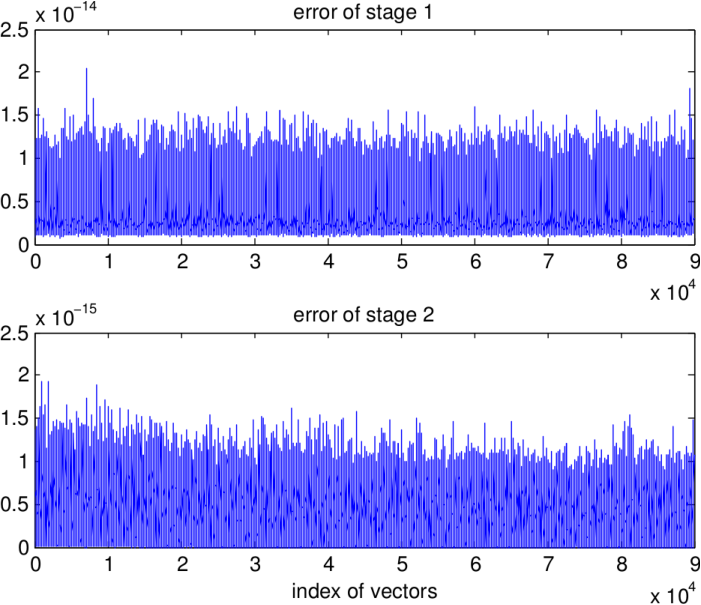
\includegraphics[width=0.7\textwidth]{err_hess_trian.pdf}
			\caption{absolute error associated with two stages, which are tested on 3000 random matrices of
			dimension $30\times 30$. The y-axis is the norm of columns of error matrices
			$E_{i}=Q^{T}_{i}M_{i}Q_{i-1}-H_{i}$ for stage 1 and $E_{i}=\hat{Q}^{T}_{i}H_{i}\hat{Q}_{i-1}=R_{i}$
			for stage 2, so there are total $3000*30=90000$ points. The x-axis is the indices
			of these columns.
			}
			\label{fig:err_hess_trian}
		\end{figure}

		\paragraph{Stage 2}
		The transition from second row to the third row in \ref{fig:per_schur_algorithm} is the second stage.
		\begin{itemize}
			\item input: upper-triangular matrices $H_{2},H_{1}$ and upper-hessenberg matrix $H_{3}$.
			\item output: upper-triangular matrices $R_{2}, R_{1}$ and quasi-upper triangular matrix $R_{3}$.\\
					orthogonal matrices $\hat{Q}_{3},\hat{Q}_{2},\hat{Q}_{1}$, such that
					$\hat{Q}^{T}_{i}H_{i}\hat{Q}_{i-1}=R_{i}$,
					$\hat{Q}_{0}=\hat{Q}_{3}$.
		\end{itemize}
		Stage 2 is called ``periodic QR'' step in paper \rf{Bojanczyk92theperiodic} because the basic process
		in this stage is conducting QR iteration periodically, which is an extension of ``Francis's Algorithm''
		in the singe matrix case. The convergence of this stage is guaranteed by
		\HREF{http://people.inf.ethz.ch/arbenz/ewp/Lnotes/chapter3.pdf}{``Implicit Q theorem''}.
		For each iteration, the number of each Givens rotation is $O(mN)$, and the cost of Givens rotation
		is roughly $O(N)$, so the cost of each iteration is $O(mN^{2})$, which seems very cheap at the first
		glance. However,
		the converging rate of this stage is a not that optimistic, at least for \KS\ system.

		Paper \rf{Bojanczyk92theperiodic} introduces two different shift methods in this stage so as to get a
		better converging rates: \textit{single-shift step} and \textit{double-shift step}. But for me,
		choosing the appropriate shift is just like black magic and all my trials just backfire, so I choose
		not to use shift at all in my code. Maybe I should have put enough effort in this stage.
		If someone can find a reliable method to select the shift, hope you can tell me.
			
		Again, the numerical error associated with stage 2 is small as shown in Fig \ref{fig:err_hess_trian},
		which is the result of a test on a product of 3000 matrices.

		\paragraph{Note} The original algorithm consists of 4 stages, but I only introduce 2 of them because these
		2 stages are enough for \KS\ system. The other two stages are \textit{Deflation} and \textit{Eigenvalues
		reodering}. When the matrix product is singular, we need to get rid of zero elements on the diagonal of these
		upper-triangular matrices, where \textit{Deflation} is used. In this sense, \psd\ can be used for singular
		matrix too, but I don't think Jacobian matrix of \KSe\ is singular. At the same time, the Floquet multipliers
	 	are ordered by themselves for \KS\ system, so there is no need to reorder the eigenvalues.

	\subsubsection{Eigenvalues}
		Assume that stage 2 is accomplished and we have $m$ matrices: $M_{1},M_{2},\cdots,M_{m}$,
		the first $m-1$ of which are upper-triangular matrices and the last one is quasi-upper triangular matrix.
		It is time to calculate the eigenvalues right now.

		The process is quite simple. If the $i_{th}$ eigenvalue is real, then it is just the product of all the $i_{th}$
		diagonal elements of matrices $M_{1},M_{2},\cdots,M_{m}$. In practice, the logarithm of these numbers is added
		to overcome overflow or downflow. If the $i_{th}$ and $(i+1)_{th}>$ eigenvalues are complex conjugate pairs,
		we just need to multiply all the $2\times 2$ matrices at position $(i,i+1)$ on the diagonal, and the two
		eigenvalues of this product are what we need. There is no danger of overflow because all these $2\times 2$
		matrices are in the same position and their elements should have similar order of magnitude, which is at least
		true for \KS\ system.

	\subsubsection{Eigenvectors}
		My method to calculate eigenvectors is based on power iteration and the prerequisite is that all the eigenvalues
		are ordered in ascending or descending order by their magnitude. This method cannot deal with degenerate case, but
		it is capable to get the complex eigenvector pair.

		Suppose the \psd\ of $J=M_{m}\cdots M_{2}M_{1}$ is $Q^{T}_{m}JQ_{m}=R_{m}\cdots R_{2}R_{1}$, where $Q_{m}$ is an
		orthogonal matrix, $R_{m-1},\cdots, R_{2},R_{1}$ are upper-triangular matrices and $R_{m}$ is quasi-upper triangular.
		We only need to calculate eigenvectors $v_{i}, i=1,2\cdots, N$ of matrix $R=R_{m}\cdots R_{2}R_{1}$
		because eigenvectors of $J$ are related to $v_{i}$ by $Q_{m}$. The basic idea is that \textbf{the eigenvector matrix
		[$v_{1}$,$v_{2}$,$\cdots$,$v_{N}$] of a quasi-uppper triangular matrix is quasi-upper triangular too}.
		
		\paragraph{Real eigenvectors}
			If the $i_{th}$ eigenvector is real, then it has the form
			\begin{center}
				$v_{i}=(a_{1},a_{2},\cdots,a_{i},0,\cdots, 0)^{T}$.
			\end{center}
			First, Let's assume that all the eigenvalues are ordered ascend:
			$|\ExpaEig_{1}|<|\ExpaEig_{2}|<\cdots<|\ExpaEig_{N}|$.
			An arbitrary vector whose first $i$ elements are nonzero $x=(b_{1},b_{2},\cdots,b_{i},0,\cdots, 0)^{T}$
			is a linear combination of the first $i$ eigenvectors.
			\begin{center}
				$x=\alpha_{1}v_{1}+\alpha_{2}v_{2}+\cdots+\alpha_{i}v_{i}$.
			\end{center}
			Use it as the initial guess for the power iteration and after $k$ iterations:	
			\[
			R^{k}x=\ExpaEig_{i}^{k}(\alpha_{1}\frac{\ExpaEig_{1}^{k}}{\ExpaEig_{i}^{k}}v_{1}
					+\alpha_{2}\frac{\ExpaEig_{2}^{k}}{\ExpaEig_{i}^{k}}v_{2}
					+\cdots
					+\alpha_{i}v_{i})
			\]
			It is clear to see that if this vector is normalized after each iteration, then it will converge to the
			$i_{th}$ eigenvector of $R$:
			\[
			\lim_{k\to \infty} \frac{R^{k}x}{|R^{k}x|}=v_{i}
			\]

			Second, Let's assume that all the eigenvalues are ordered descend:
			$|\ExpaEig_{1}|>|\ExpaEig_{2}|>\cdots>|\ExpaEig_{N}|$.
			Since $Rv_{i}=\ExpaEig_{i}v_{i}$, then $R^{-1}v_{i}=\ExpaEig_{i}^{-1}v_{i}$. $R$ and $R^{-1}$ have the
			same set of eigenvectors with reciprocal eigenvalues, so the eigenvalues of
			$R^{-1}=R_{1}^{-1}R_{2}^{-1}\cdots R_{N}^{-1}$ are ordered ascend. We go back to the first case!
			I use this method to get {\cLvs} for \KS\ system. Note that this process is numerically
			practicable because each $R_{i}$ is well conditioned if the time step is small enough.

			What if the eigenvalues are not ordered ascend or descend ? I just omit this situation because the
			eigenvalues for \KS\ system are ordered descend, but I think you need to reorder eigenvalues in the
			\psd\ .

		\paragraph{Complex eigenvector pair}
			The eigenvectors corresponding to the complex eigenvalues are complex and they appear as pairs.
			Power iteration will fail in this case because now two eigenvalues have the same magnitude:
			$\ExpaEig_{i}$ and $\ExpaEig_{i}^{*}$. If you start the power iteration with a real vector, then
			you will find that it is stretching or contracting in an oscillating style.
			
			We can introduce complex shift to resolve this problem. Let the $i_{th}$ eigenvalue to be
			$\ExpaEig_{i}=a+ib$, where $b>0$, then the $(i+1)_{th}$ eigenvalue is $\ExpaEig_{i+1}=a-ib$. It is obvious
			that $R+is\mathbf{I}$ and $R$ have the same eigenvectors, where $s$ is an arbitrary real number.
			\begin{align*}	
			(R+is\mathbf{I})v_{i} & =[a+i(b+s)]v_{i}\\
			(R+is\mathbf{I})v_{i+1} & =[a+i(-b+s)]v_{i+1}
			\end{align*}	
			So $R+is\mathbf{I}$ can be used in the power iteration instead of $R$. If $s>0$, it will converge to $v_{i}$
			since $b>0$. If $s<0$, it will converge to $v_{i+1}$.

			One point should be stressed. If $v_{i}$ is the eigenvector corresponding to $\ExpaEig_{i}=a+ib$, then
			$e^{i\theta}v_{i}$ is also an eigenvector corresponding to the same eigenvalue, where $\theta$ is an
			arbitrary real number. In this sense, complex eigenvector is not defined uniquely. In my code, I just force
			the first element of complex eigenvector to be real, and then this vector is determined precisely.
			
			The choice of shift $s$ is based on the criteria that it should split the magnitudes of these two eigenvalues
			as large as possible so that the converging process is fast.

		



\subsection{Floquet exponents and {\cLvs}}

	Now we apply \psd\ to \KS\ system. In this part, I will exhibit the Floquet
	exponents and  the {\cLvs} for two pre-\po s of
	\KSe: \cycle{ppo1} and \cycle{ppo9} in Ruslan's data file:
\\
	\texttt{siminos/matlab/ruslan/ks22f90h25t100.mat}. $\cycle{ppo1}$ has a prime
	period $\period{ppo1}=10.25\cdots$ and $\cycle{ppo9}$ has a prime period $\period{p9}=41.55\cdots$.
	\refFig{fig:ppo19_phase123} shows the configuration of these two orbits evolved
	for their prime periods respectively, and it shows that the  full period is twice
	the prime period in both cases.

	The group operation that transforms $x(0)$ to
	$x(t_{p})$ is reflection: $Ru(x)=-u(-x)$, which is
	\begin{align*}	
	R \, \Re a_{i} & =-\Re a_{i} \qquad i \mbox{odd}\\
	R \, \Im a_{i} & =\Im a_{i}  \qquad i \mbox{even}
	\end{align*}
	in Fourier coefficient space. Therefore, the group representation in both cases is
	\[
	g_{p}=diag(-1,1,-1,1,\cdots)
	\]
	\begin{figure}%[h]
	\centering
		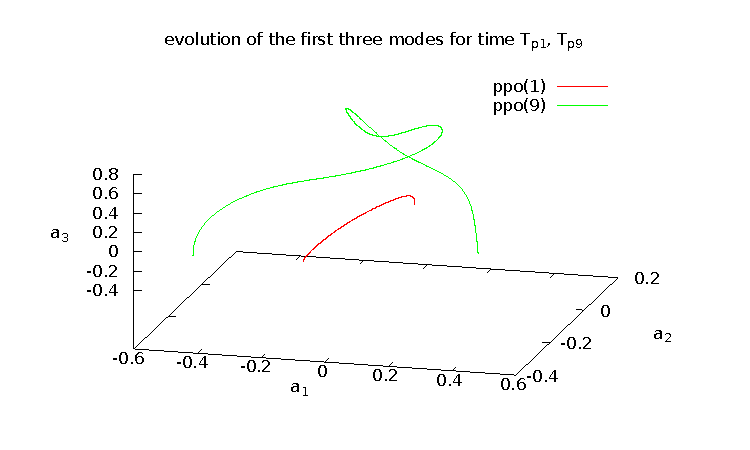
\includegraphics[width=0.8\textwidth]{ppo19_phase123.pdf}
		\caption{Demonstration of the evolution of the first
		three Fourier coefficients for pre-\po s \cycle{ppo1} and \cycle{ppo9}.
		}
		\label{fig:ppo19_phase123}
	\end{figure}
	
	\paragraph{Relation between $g_{p}J^{\period{p}}$ and $J^{2\period{p}}$}
		I will give my result for Floquet exponents and
		{\cLvs} by two different matrices: $g_{p}J^{\period{p}}$ and
		$J^{2\period{p}}$. The former one is the definition of Jacobian matrix for
		relative periodic orbits, while the latter is just the Jacobian matrix for
		the full period, so we need to know their relation first.
		
		The orbits $\cycle{ppo1}$ and $\cycle{ppo9}$ are equivariant under group operation
		$g_{p}$:
		\[
		g_{p}f^{\period{p}}(x(0))=f^{\period{p}}(g_{p}x(0))
		\]
		where $f^{t}(x)$ is the flow equation of \KS\ system. Take the derivative of $x(0)$
		at both side and use the definition of Jacobian matrix
		$J^{t}(x)=\frac{\partial f^{t}(x)}{\partial x}$ , we have
		\[
		g_{p}J^{\period{p}}(x(0))=J^{\period{p}}(g_{p}x(0))g_{p}
		\]
		Therefore,
		\begin{align*}
			 J^{2\period{p}}(x(0)) & =J^{\period{p}}(x(\period{p}))J^{\period{p}}(x(0))	\\	
			& =J^{\period{p}}(g_{p}x(0))J^{\period{p}}(x(0))\\
			& =J^{\period{p}}(g_{p}x(0))g_{p}g_{p}J^{\period{p}}(x(0))\\
			& =g_{p}J^{\period{p}}(x(0))g_{p}J^{\period{p}}(x(0))
			  =(g_{p}J^{\period{p}}(x(0)))^{2}\,.
		\end{align*}
		During the process, I used the identity $g_{p}^{2}=\mathbb{I}$
        for reflection symmetry group $\Dn{2}$. Define
		\begin{equation}
		J_{p}=g_{p}J^{\period{p}}
		\label{eq:relative_jacobian}
		\end{equation}
		so we have relation:
		\begin{equation}
			J^{2\period{p}}=(J_{p})^{2}
		\label{eq:relationofjpj2t}
		\end{equation}
		Therefore, these two matrices have the same eigenvectors and the
eigenvalues of $J^{2\period{p}}$ are just square of the
corresponding ones of $J_{p}$, which means all the real eigenvalues of
$J^{2\period{p}}$ are positive. I will check this relation in the
following sections.
            \PC{Eventually, you want to make this argument totally
            general and simpler: I think you only need to know that the symmetry
            group actions commute with the dynamics, and for pre-periodic
            prime orbits (in case of discrete symmetries) the identity
            $g_{p}^{m}=\mathbb{I}$. How about reading
            \HREF{http://www.streamsound.dk/book1/chaos/chaos.html\#184/z}
            {ChaosBook} :)
                }
		
	\subsubsection{Floquet exponents}
		Floquet multipliers $\ExpaEig_{i}$ are defined as the eigenvalues of Jacobian matrix for periodic
		orbit. For relative periodic orbits, Jacobian is defined in \eqref{eq:relative_jacobian}.
		Floquet exponents $\lambda_{i}$ are defined as
        $\ExpaEig_{i}=\exp\left(\period{p}\Lyap_{i}\right)$. If Floquet exponent
        is complex, then it is written as
        $\Lyap_{i}=\eigRe[i]+i\eigIm[i]$.
		\refTab{tab:FloqExpPPO1} contains the Floquet exponents I got for the orbit $\cycle{ppo1}$ with
		respect to two different methods: one evolves the system for $\period{p1}$ and conducts group transformation;
		the other just evolves the system for $2\period{p1}$.
            \PC{
            Why plot $e^{i\period{p}\eigIm[i]}$? The $\pm$ sign is the
            character of $g_{p}$, and you want to show that the two
            $\eigIm[i]$ are the same, not compare $\cos \eigRe[i]$ with
            $\cos 2\eigRe[i]$? That serves no purpose. \eigRe[i] and \eigIm[i]
            are \emph{rates per unit time}, they are the same for any repeat of the
            the prime orbit.
                }
		
\input ../xiong/tables/FloqExpPPO1
		
\refTab{tab:FloqExpPPO1} shows that there are two complex eigen-pairs:
$(1,2)$ and $(6,7)$. All the other exponents are real. There are several
points needed to be stressed.

		\paragraph{Error analysis of the result}
		From previous analysis and \eqref{eq:relationofjpj2t}, we know that the first column should be the same
		with the third column in \reftab{tab:FloqExpPPO1}, and the square of second column should
		coincide with the fourth column. The observation is that these two relation is confirmed in a certain
		degree, but the accuracy is only about $10^{-4}$. It looks pessimistic
		to get such a large error, but we should locate the sources of this error before casting some doubt on
		\psd\ .
		
		The error has two sources:
		the \KSe\ solver and the \psd\ algorithm described here.
		Theoretically, the orbit transformed by $g_{p}$ after evolving for $\period{p}$ should coincide with the orbit
		after evolving for $2\period{p}$. But I find that
		\[
		|g_{p}f^{\period{p}}(x(0))- f^{2\period{p}}(x(0))|=2.627440335452566e-04		
        \,,
        \]
which has just the same magnitude of the total error. Therefore, there is
a great likelihood that the total error mainly comes from \KSe\ solver.

		On the other hand, we can check the error associated with \psd\ separately.
		\begin{figure}[h]
			\centering
			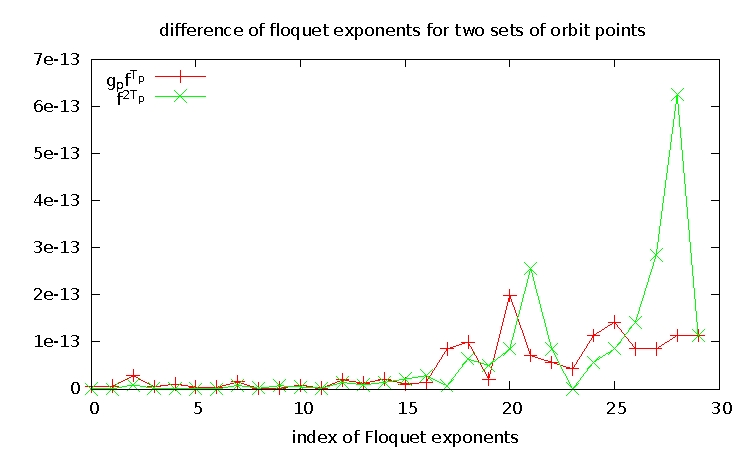
\includegraphics[width=0.8\textwidth]{err_psd.pdf}
			\caption{Difference of Floquet exponents. Red line: the prime orbit is partitioned into 500 and
			1000 segments respectively. Evolve the system for $\period{p}$
			and calculate the corresponding Floquet exponents. The red line shows the difference of
			their magnitudes pair wisely. Green line: the full orbit is partitioned into 1000 and 2000
			segments respectively and evolve the system for $2\period{p}$.}
			\label{fig:err_psd}
		\end{figure}
		Fig \ref{fig:err_psd} clearly shows that the error originated from \psd\ is around $10^{-13}$.We
		are relieved now!

		\paragraph{Observations}

		\begin{figure}[h]
			\centering
			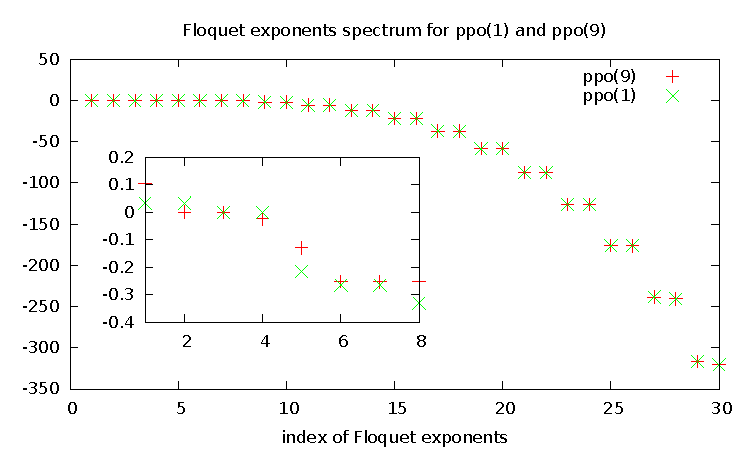
\includegraphics[width=0.8\textwidth]{floquet_spectrum19.pdf}
			\caption{ Floquet exponent spectrum for prime orbit $\cycle{ppo1}$ and $\cycle{ppo9}$.
			The inner graph is the magnification of the first 8 exponents. For these complex exponents,
			just take $\mu_{i}$ as defined before.
			}
			\label{fig:floquet_spectrum19}
		\end{figure}
		
			Table \ref{tab:FloqExpPPO1} tells us that Floquet exponent could be negative, which
			means the corresponding eigenvector reverses its direction after one prime period. Also it
			could be complex pair, which means that any vector in its eigenspace  will rotate inside this
			subspace.

			\refFig{fig:floquet_spectrum19} shows $\mu_{i}$ (the first column in table
			\ref{tab:FloqExpPPO1}) for prime orbit $\cycle{ppo1}$ and $\cycle{ppo9}$. $9_{th}$ to
			$30_{th}$ floquet exponents are almost the same for both orbits (proportional to the
			forth order of Fourier mode index). $(1,2)$ and $(6,7)$ are two pairs of complex
			Floquet exponents for $\cycle{ppo1}$; while orbit $\cycle{ppo9}$ has only one complex pair: $(7,8)$.





	\subsubsection{\cLvs}
	
	\paragraph{Configuration}
		\refFig{fig:ppo1ev_low} and \ref{fig:ppo1ev_high} show the configuration of some {\cLvs} for \KS\ system,
		which clearly shows that the {\cLvs} corresponding to high Fourier modes are just localized around
		its mode index; while the first few {\cLvs} spread among first few indices.
		\begin{figure}[h]
		\centering
			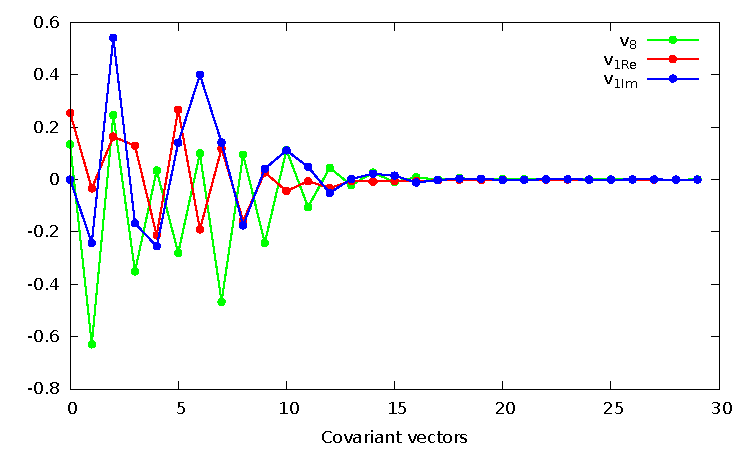
\includegraphics[width=0.9\textwidth]{ppo1ev_low.pdf}
			\caption{The $1_{st}$ and $8_{th}$ \cLvs for the \cycle{ppo1} orbit ($\period{P}=10.25\cdots$).
			X-axis is the index of the elements of a vector.
			}
			\label{fig:ppo1ev_low}
		\end{figure}

		\begin{figure}[h]
		\centering
			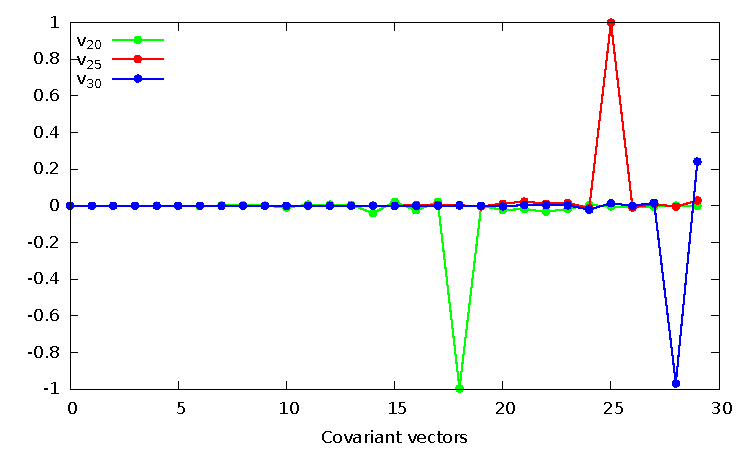
\includegraphics[width=0.9\textwidth]{ppo1ev_high.pdf}
			\caption{The $20_{th}$, $25_{th}$ and $30_{th}$ \cLvs for the \cycle{ppo1} orbit ($\period{P}=10.25\cdots$).
			X-axis is the index of the elements of a vector.
			}
			\label{fig:ppo1ev_high}
		\end{figure}

	\paragraph{Expansion/contraction rate of \cLvs}
		When {\cLvs} evolve along the orbit, their expansion/contraction rate is recorded. \refFig{fig:ppo1rate}
		shows that the $8_{th}$ vector behaves well along the orbit, and the contraction rate is obviously periodic.
		While, vector $v_{10}$ is contaminated by other more expanding vectors after a short time. \Xiongedit{Kazz: This means that your choice of the time step and/or the interval between two Gram-Schmidt orthonormalization is not short enough. You have to set them to be, at the longest, $\mathcal{O}(|\lambda|_{\rm max}^{-1})$, where $|\lambda|_{\rm max}$ is the largest absolute value of the Lyapunov exponent you are interested in (here it is set by the most negative Lyapunov exponent).}
		\begin{figure}[h]
		\centering
			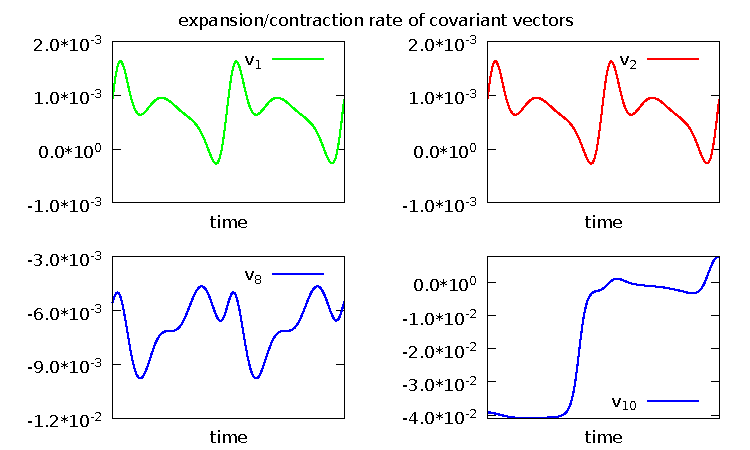
\includegraphics[width=1.0\textwidth]{ppo1rate.pdf}
			\caption{ The expansion/contraction rate of several {\cLvs} for orbit \cycle{ppo1}. The x-axis is time and
			time step is $\period{p}/1000$. Y-axis is logarithm the expansion rate of these vectors along the orbit. The total
			time is $2\period{p}$.
			}
			\label{fig:ppo1rate}
		\end{figure}
	
	\paragraph{Vector field }
		For periodic orbit, the velocity coincides with the \cLv\ that corresponds to
		a marginal Floquet multiplier. \refTab{tab:FloqExpPPO1} shows there are two
		marginal Floquet multipliers for orbit \cycle{ppo1}: $3_{rd}$ and $4_{th}$. The evolution of the third covariant
		vector is shown in \refFig{fig:ppo1vectorfield123}, from which we can conclude this
		{\cLv} is just the local velocity along the orbit.
		
		The same goes for orbit \cycle{ppo9}. In this case, the second \cLv\ represents the local
		velocity along the orbit, which is demonstrated in \refFig{fig:ppo9vectorfield123}.
		\begin{figure}[h]
		\centering
			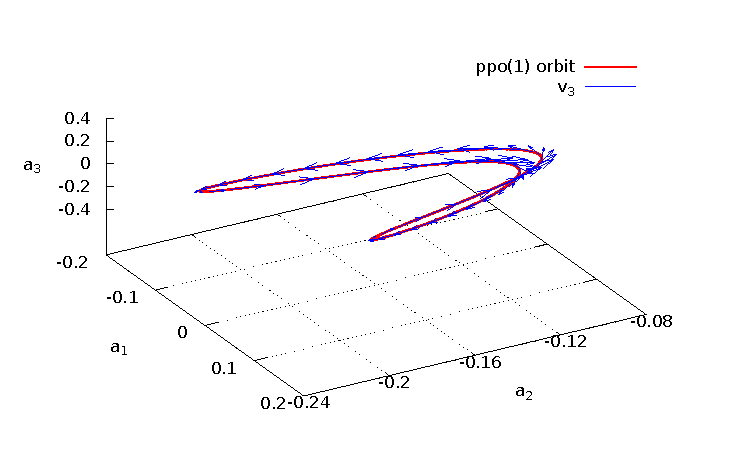
\includegraphics[width=1.0\textwidth]{ppo1vectorfield123.pdf}
			\caption{The orbit \cycle{ppo1} and the evolution of the third \cLv. X, Y and Z axis
			are the first, second and third element of the state vector.
			}
			\label{fig:ppo1vectorfield123}
		\end{figure}

		\begin{figure}[h]
		\centering
			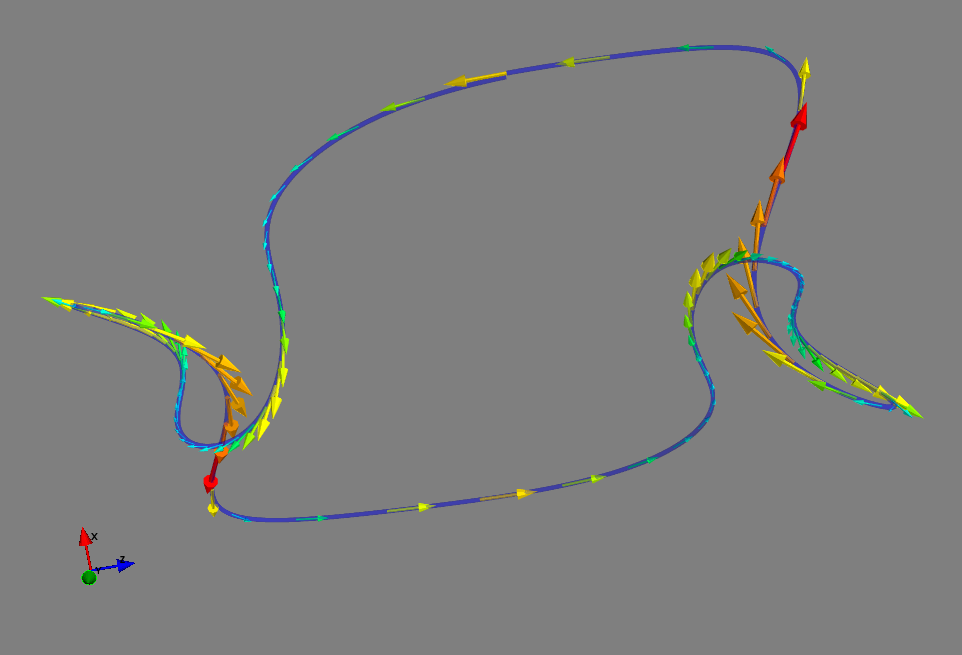
\includegraphics[width=1.0\textwidth]{ppo9vectorfield_mlab.png}
			\caption{The orbit \cycle{ppo9} and the evolution of the second \cLv\. X, Y and Z axis
			are the first, second and third element of the state vector.
			}
			\label{fig:ppo9vectorfield123}
		\end{figure}

\begin{figure}[h]
  \centering
  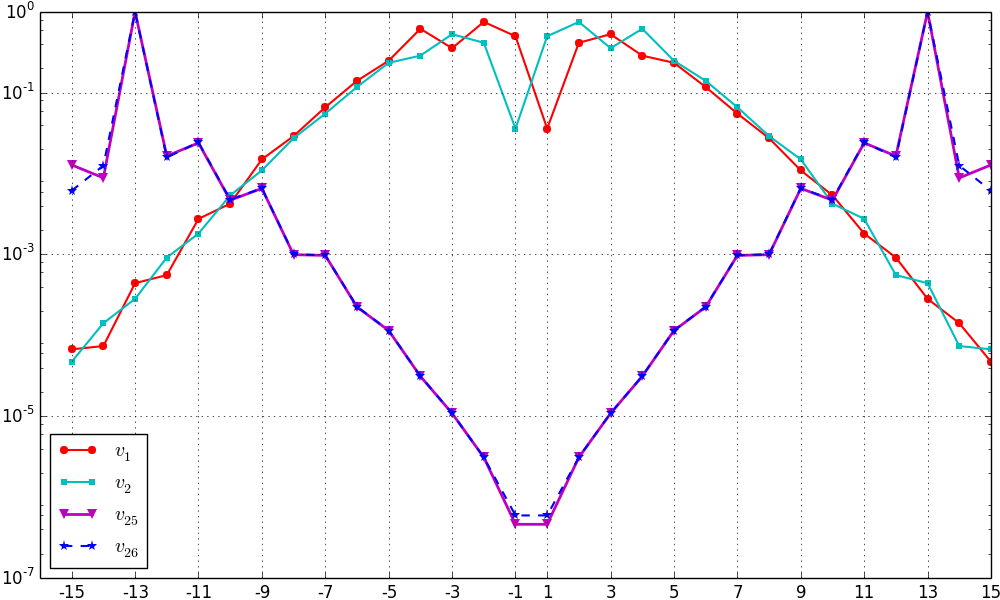
\includegraphics[width=1.0\textwidth]{ppo1FloquetVector}
  \caption{The 1st, 2nd, 25th and 26th Floquet vectors of
    preperiodic orbit \cycle{ppo1} with truncation number
    $N=32$. The x-axis is the Fourier mode
    indices. Note Matlab \texttt{fft()} orders wave numbers as
    $k=0,1,2,\cdots,N-1$ which is mapped to
    $k=0,1,\cdots,N/2-1,N/2,-N/2+1,\cdots,-1$ here. Also,
    mode $a_0$ and $a_{N/2}$ are ignored here because they are set to
    zero at the very beginning.
    Each Fourier mode
    has a real and imaginary part: $a_k=b_k+ic_k$. Floquet vectors
    are calculated in space $[b_1, c_1,\cdots,b_{N/2-1},c_{N/2-1}]$
    first and then their modulus at each mode is obtained:
    $|a_{k}|=|b_k+ic_k|$. Also note only half of them are needed since
    $a_{-k}=b_{k}-ic_{k}$. If Floquet vector is real ($v_{25}$, $v_{26}$),
    then $|a_{k}|=|a_{-k}|$, that is, they are self-dual under reflection
    along $x=0$.
    If Floquet vectors form complex conjugate pair ($v_1$, $v_2$), then
    there are relations
    $b^{(1)}_{k}=(b^{(2)}_{k})^{*}$ and $c^{(1)}_{k}=(c^{(2)}_{k})^{*}$,
    so
    $
    |a_{k}^{(1)}|=|b_k^{(1)}+ic_{k}^{(1)}|=|(b_{k}^{(1)})^{*}-i(c_{k}^{(1)})^{*}|
    =|b_k^{(2)}-ic_{k}^{(2)}|
    =|a_{-k}^{(2)}|
    \,.
    $
    Therefore, $v_1$ is dual to $v_2$ under reflection in this figure.
    In summary, actually, only half of the this figure is enough.
    This figure is different from \reffig{fig:ppo1ev_low} and
    \ref{fig:ppo1ev_high}, which are just
    $N-2$ components ($b_1, c_1,\cdots,b_{N/2-1},c_{N/2-1}$)
    of Floquet vectors.
  }
  \label{fig:ppo1FloquetVector}
\end{figure}

\clearpage
\subsection{Floquet Vectors by Reordering}

The iteration algorithms used before (Ginelli's algorithm
\rf{GiChLiPo12} or my first algorithm described above)
 all suffer two drawbacks (I am sorry I am trying to use
an appropriate word here, so you can choose another
 one if it is better ).

\begin{itemize}
\item Convergence depends on how large the gaps between eigenvalues
  of Jacobian matrix are. For
  Jacobian associated with periodic orbits in \KS\ system, multipliers
  appear in pairs, so iteration algorithm converges slowly in order to
  distinguish these pairs. We can use shift iterations to accelerate
  the convergence process when dealing with periodic orbits
  ( shift iterations has not been documented
  in Genelli's paper because he is talking about ergodic orbits. Maybe I
  should write it down in the blog \Xiongedit{(Kazz: yes, please!)}, but convergence requires
  the combination of ``shift power iteration'' and  ordinary power
  iteration, which is also a little expensive for some cases such
  as the two marginal eigenvectors.

\item We cannot get all the Floquet vectors along the orbit by
  just evolving
  Floquet vectors because of the noise introduced to the unstable
  Floquet vectors under time evolution. Therefore, iteration is
  needed at each point along
  the orbit. Even though we can use the Floquet vectors at present
  point as a good initial condition for the iteration at the next point,
  the iteration process cannot be omitted. Think about a orbit which
  consists of 8000 points, the iteration method is expensive.
\end{itemize}

Additionally, Genelli's algorithm has another defect(?): it cannot
distinguish degenerate multipliers or complex multiplier pairs.

Now I introduce a direct algorithm to get all the Floquet vectors
along a periodic orbit at once without iteration, which is based on
\psd .

After \psd , we rewrite Jacobian matrix as
\begin{equation}
  \label{eq:xdpsd}
  J=QRQ^{T}
\end{equation}
where $Q$
is an orthogonal matrix and $R$ is a quasi-upper-triangular matrix,
so eigenvectors $e_{i}$ of $J$ is related to eigenvectors $\hat{e}_{i}$
 of $R$ by $e_{i}=Q\hat{e}_{i}$.  Now it suffices to consider $R$
only. I want to share with you a very simple observation:
\textbf{The eigenvector corresponding to the first diagonal element
of an upper-triangular matrix is $e_{1}=(1,0,\cdots,0)^{T}$}, so
if we can reorder the diagonal elements (or 2x2 blocks) of $R$, then
we can find any eigenvector by just positioning the corresponding
eigenvalue in the first diagonal position.

paper \rf{GranatK06} talks about the general case: reordering of two
blocks of an upper-triangular matrix. For our purpose, we only
consider two simpler specific cases: reordering of 1x1 and 2x2
blocks. Now I introduce the basic idea of this algorithm.

\subsubsection{Periodic Sylvester equation}
After conducting \psd , we rewrite Jacobian matrix as form
 \eqref{eq:xdpsd}. Usually, $R$ is not a single matrix but
a product of upper-triangular or quasi-upper-triangular
matrices
\begin{equation}
R=R_{m}R_{m-1}\cdots R_{1}
\label{eq:xduppertriangular}
\end{equation}
where $R_{m}$ is quasi-upper-triangular while $R_{1,2,\cdots,m-1}$ is
upper-triangular.

denote $R_{i}$ as
\[
R_{i}=
\left[
\begin{array}{c|cc|c}
  R^{00}_{i} & * & *& * \\ \hline
  0 & R^{11}_{i} & R^{12}_{i} & * \\
  0 & 0 & R^{22}_{i} & * \\ \hline
  0 & 0 & 0 & R^{33}_{i}
\end{array}
\right]
\]
Where $R^{00}_{i}, R^{11}_{i},R^{22}_{i},R^{33}_{i}$ have size
$p0\times p0,p1\times p1,p2\times p2,p3\times p3$ respectively,
 and $p0+p1+p2+p3=m$.

In order to exchange the middle two blocks ($R^{11}_{i}$
and $R^{22}_{i}$), we construct a non-singular matrix sequence:
$\hat{S_{i}}\quad i=0,1,2,\cdots,m$ with $\hat{S_{0}}=\hat{S_{m}}$.
\[
\hat{S_{i}}=
\left[
\begin{array}{c|c|c}
  I_{p0} & 0 & 0  \\ \hline
  0 & S_{i} & 0 \\ \hline
  0 & 0 & I_{p3}
\end{array}
\right]
\]

such that $\hat{S}_{i}$ transforms $R_{i}$ like:
\begin{equation}
\label{eq:xdtransform}
\hat{S}_{i}^{-1}R_{i}\hat{S}_{i-1}=\tilde{R}_{i}=
\left[
\begin{array}{c|cc|c}
  R^{00}_{i} & * & *& * \\ \hline
  0 & R^{22}_{i} & 0 & * \\
  0 & 0 & R^{11}_{i} & * \\ \hline
  0 & 0 & 0 & R^{33}_{i}
\end{array}
\right]
\end{equation}

which is
\[
S^{-1}_{i}
\left[
\begin{array}{c c}
  R^{11}_{i} & R^{12}_{i} \\
  0 & R^{22}_{i}
\end{array}
\right]
S_{i-1}=
\left[
\begin{array}{c c}
  R^{22}_{i} & 0 \\
  0 & R^{11}_{i}
\end{array}
\right]
\]

The problem turns to be finding appropriate matrix $S_{i}$ which satisfies
the above equation. Assume $S_{i}$ has form
\[
S_{i}=
\left[
\begin{array}{c c}
  X_{i} & I_{p1} \\
  I_{p2} & 0
\end{array}
\right]
\]
where matrix $X_{i}$ has dimension $p1\times p2$, then we get equation
\begin{equation}
  \label{eq:xdpse}
  R^{11}_{i}X_{i-1}-X_{i}R^{22}_{i}=-R^{12}_{i} \quad i=0,1,2,\cdots,m
\end{equation}

Equation \eqref{eq:xdpse} is called \textbf{Periodic Sylvester Equation}.

The algorithm to find eigenvectors is based on \eqref{eq:xdpse}. If the
$i_{th}$ eigenvalue of $R$ is real, we only need to exchange the first
$(i-1)\times (i-1)$ block of $R$ with its $i_{th}$ diagonal element.
If the $i_{th}$ and $(i+1)_{th}$ eigenvalues are complex pair, then
the first $(i-1)\times (i-1)$ block and the following $2\times 2$
block should be exchanged. Therefore $X_{i}$ in \eqref{eq:xdpse}
has dimension $p1\times 1$ or $p1\times 2$.

\subsubsection{Real eigenvector}
In this case, matrix $X_{i}$ is just a column vector, so
\eqref{eq:xdpse} is equivalent to
\begin{equation}
  \label{eq:xdpsereal}
  \begin{bmatrix}
    R^{11}_{1} & -R^{22}_{1}I_{p1} &  & \\[1em]
    & R^{11}_{2} & -R^{22}_{2}I_{p1} &  &\\[1em]
    &  & R^{11}_{3} & -R^{22}_{3}I_{p1} &  &\\[1em]
    & & & \ddots &\cdots & \\[1em]
    -R^{22}_{m}I_{p1} & & & & R^{11}_{m}
  \end{bmatrix}
  \begin{bmatrix}
    X_{m} \\[1em]
    X_{1}  \\[1em]
    X_{2}  \\[1em]
    \cdots \\[1em]
    X_{m-1}
  \end{bmatrix}
  =
  \begin{bmatrix}
    -R^{12}_{1} \\[1em]
    -R^{12}_{2} \\[1em]
    -R^{12}_{3} \\[1em]
    \cdots \\[1em]
    -R^{12}_{m}
  \end{bmatrix}
\end{equation}
Where, $R^{22}_{i}$ is just the $(p1+1)_{th}$ diagonal element of $R_{i}$.
This is a bordered almost block diagonal (BABD) matrix, which has
dimension $(p1*m)\times (p1*m)$; by the way, The multi-shooting
 matrix has the same structure\ES{You might want to look at Numerical
 Recipies for Woodbury's formula. I've used it to solve similar systems
 of equations arising in ``Newton's descend''\rf{lanVar1} efficiently.
 It is an exact, not an iterative method.}.

I chose to use Gaussian  elimination with partial pivoting (GEPP)
to solve \eqref{eq:xdpsereal}. a few people \rf{NLA:NLA198} argue
that GEPP is not
stable for some matrices, and other methods have been proposed
\rf{aabdls,GranatRBA}. As far as I'm concerned, GEPP is stable for
\eqref{eq:xdpsereal} if the time step in \KS\ integrator is
not too large, because GEPP only uses addition and subtraction
operations.

Now we get all vectors $X_{i}$ by solving \pse\ , but how are they
related to the eigenvectors ?

Define $\tilde{R}=\tilde{R}_{m}\tilde{R}_{m-1}\cdots\tilde{R}_{1}$,
we get
$\hat{S}_{m}^{-1}R\hat{S}_{m}=\tilde{R}$ by \eqref{eq:xdtransform}.
Since $p0=0$ and $p2=1$ in \eqref{eq:xdtransform}, the first
eigenvector of $\tilde{R}$, the one corresponding
 to eigenvalue $R^{22}$, is
$\tilde{e}=(1,0,\cdots , 0)^{T}$. Therefore, the corresponding
eigenvector of $R$ is
\[
e=\hat{S}_{m}\tilde{e}
 = \left[
   \begin{array}{c}
   X_{m} \\
   1    \\
   0 \\
   0\\
   \vdots\\
   0
   \end{array}
 \right]
\]
This is the eigenvector of matrix $R=R_{m}R_{m-1}\cdots R_{1}$ at the
initial point of the orbit. Now I explain why \pse\ gives all
the eigenvectors along the orbit. For the next point along the orbit,
$R=R_{1}R_{m}\cdots R_{2}$, therefore the \pse\ will be rotated one row up,
which means $X_{1}$ will be shifted to the first place in the column
vector in \eqref{eq:xdpsereal}; in this way, the corresponding
eigenvector of $R$ is $e=(X_{1},1,0,\cdots,0)^{T}$. The same
argument goes for all the following points along the orbit. In conclusion,
solution of \eqref{eq:xdpsereal} contains all the eigenvectors along the
orbit.

\subsubsection{Complex Eigenvector Pair}
The complex eigenvector case is more twisted than the real one. Again
we have $p0=0$, but now $p2=2$, so the matrix $X_{i}$  has dimension
$p1\times 2$. Let $v(X_{i})$ denote the vector representation of $X_{i}$
with the columns of $X_{i}$ stacked on top of each other, and let
$A\otimes B$ denote the Kronecker product of two matrices, with the
 $(i,j)$-block element be $a_{ij}B$.

Now, the \pse \eqref{eq:xdpse} is equivalent to
\begin{equation}
  \label{eq:xdpsdcomplex}
  \resizebox{\linewidth}{!}{%
  $
  \setlength{\arraycolsep}{3pt}
  \begin{bmatrix}
    I_{2}\otimes R^{11}_{1} & -(R^{22}_{1})^{T}\otimes I_{p1} &  & \\[1em]
    & I_{2}\otimes R^{11}_{2} & -(R^{22}_{2})^{T} \otimes I_{p1} &  &\\[1em]
    &  & I_{2}\otimes R^{11}_{3} & -(R^{22}_{3})^{T}\otimes I_{p1} &  &\\[1em]
    & & & \ddots &\cdots & \\[1em]
    -(R^{22}_{m})^{T}\otimes I_{p1} & & & & I_{2}\otimes R^{11}_{m}
  \end{bmatrix}
  \begin{bmatrix}
    v(X_{m}) \\[1em]
    v(X_{1})  \\[1em]
    v(X_{2})  \\[1em]
    \cdots \\[1em]
    v(X_{m-1})
  \end{bmatrix}
  =
  \begin{bmatrix}
    -v(R^{12}_{1}) \\[1em]
    -v(R^{12}_{2}) \\[1em]
    -v(R^{12}_{3}) \\[1em]
    \cdots \\[1em]
    -v(R^{12}_{m})
  \end{bmatrix} $%
}
\end{equation}

After switching $R^{11}_{i}$ and $R^{22}_{i}$, we can get the first two
eigenvectors of $\tilde{R}$ by multiplying the first 2x2 diagonal blocks
of $\tilde{R_{i}}$: $R^{22}=R^{22}_{m}R^{22}_{m-1}\cdots R^{22}_{1}$.
Let the eigenvectors of $R^{22}$ are $v$ and $v^{*}$, then the
corresponding eigenvector of $\tilde{R}$ are
$\tilde{e}_{1}=(v,0,0,\cdots,0)$ and
$\tilde{e}_{2}=(\tilde{e}_{1})^{*}$.
Therefore, the corresponding eigenvector of $R$ is
\[
[e_{1},e_{2}]=\hat{S}_{m}[\tilde{e}_{1},\tilde{e}_{2}]
 = \left[
   \begin{array}{c}
   X_{m} \\
   I_{2}    \\
   0 \quad 0\\
   0 \quad 0\\
   \vdots\\
   0 \quad 0
   \end{array}
 \right]
 [v,v^{*}]
\]

For other points along the orbit, the same argument in the real case applies
here too, so we obtain all the complex eigenvector pairs along the orbit.

\subsubsection{Summary}
Solving \pse\ enables us to get all the Floquet vectors (whatever real
or complex) along the periodic
orbits without iteration, which is the most valuable
 benefit of this algorithm.

 However, some potential problems should be
stressed. On one hand, the dimension of \psm\ can be as large as
$2mn\times 2mn$ and almost $4mn^{2}$ elements are non-zero, so it will
take up a lot of memory to load this matrix especially when the period of
the orbit is very large; on the other hand, the complexity of GEPP method
is $O(mn^2)$ flops, so when the orbit is long enough, this method may use
more time than other iteration algorithms, which only conduct matrix-vector
multiplication.

\subsection{Relation among these three Algorithms}
Until now, we have three different algorithms to calculate Floquet vectors
for periodic orbits.
\begin{itemize}
\item Ginelli's Algorithm \rf{GiChLiPo12}
\item my first algorithm based on iteration
\item My second algorithm based on \pse\
\end{itemize}

The first two are iteration methods, but the last one is a direct
algorithm. The last two are both based on \psd\ , but the first
one is based on Oseledec Splitting Theorem; therefore, the
 first one is a general
algorithm to calculate Covariant Lyapunov vectors, which can be used
for ergodic orbits; while, the last two can only be used to calculate
Floquet vectors for periodic orbits.

Now I just want to demonstrate that
all these three methods produce almost the same result with their own
strong and weak points when dealing with periodic orbits.

\vspace{2em}
\subsubsection{Ginelli's algorithm is equivalent to \psd\ }

Basically, Ginelli's algorithm has 4 stages:
\begin{itemize}
\item \textbf{Forward transient}: evolve the system for many periods and
  conduct QR decomposition at the same time
  until it converges to the \textit{forward Gram-Schmidt} vectors
  \rf{GiChLiPo12} (which are also called \textit{forward Lyapunov} vectors
  in \rf{KuPa12}. \Xiongedit{Kazz: This latter name is really bad, simply because they are not Lyapunov vectors.}
\item \textbf{Forward dynamics}: evolve the system for one period and
  record matrices Q and R along the orbit.
\item \textbf{backward transient}: use $R^{-1}$ to evolve an initial
  arbitrary upper-triangular matrix $C$ until it converges.
\item \textbf{backward dynamics}: use $R^{-1}$ to evolve $C$ for one
  more period and record $C$ along the orbit, after
  which the Covariant Lyapunov vectors are give by
  $V=QC$.
\end{itemize}

First, I will show you that the first stage will converge to Schur
decomposition of Jacobian matrix $J$ if all the Floquet multipliers are
real. Also I will propose a simple remedy for complex pairs.

Now just assume all the Floquet multipliers are real. Order
multipliers by their magnitude:
$|\Lambda_{1}|>|\Lambda_{2}|>\cdots >|\Lambda_{n}|$, and the
corresponding Floquet vectors are $e_{1},e_{2},\cdots ,e_{n}$.
It is known that power iteration of Jacobian will converge to
the first Floquet vector.
\[
 \lim_{n\to \infty }J^{n}v\to e_{1}
\]
We start with an orthonormal matrix $Q=[q_{1},q_{2},\cdots ,q_{n}]$
the first column
$q_{1}$ will converge to $e_{1}$. Let's study how the second column evolves
after $Q$ converges to $[e_{1},q_{2},\cdots , q_{n}]$.

QR decomposition is conducted as the system evolves, so $q_{2}$ is
orthogonal to $e_{1}$, which implies
\begin{align*}
q_{2}= & \sum_{i=2}^{n}\alpha_{i}[e_{i}-(e_{1}^{T}e_{i})e_{1}] \\
    = & \alpha_{2}[e_{2}-(e_{1}^{T}e_{2})e_{1}]+
    \alpha_{3}[e_{3}-(e_{1}^{T}e_{3})e_{1}]+ \cdots
\end{align*}
So,
\begin{align*}
  Jq_{2}= &\sum_{i=2}^{n}\alpha_{i}[\Lambda_{i}e_{i}-
  \Lambda_{1}(e_{1}^{T}e_{i})e_{1}] \\
  = & \sum_{i=2}^{n}\alpha_{i}\Lambda_{i}[e_{i}-
  (e_{1}^{T}e_{i})e_{1}]+\sum_{i=2}^{n}\alpha_{i}
  (\Lambda_{i}-\Lambda_{1})(e_{1}^{T}e_{i})e_{1} \\
\end{align*}
The second term in the above equation will be discarded because QR
decomposition entails the second column is orthogonal to the first
column $e_{1}$. Also the first term will converge to
 $e_{2}-(e_{1}^{T}e_{2})e_{1}$ after sufficient times of iteration.

The same argument works for the remaining columns in Q. Therefore,
after sufficient times of iteration, we get
\[
\lim_{n\to \infty}J^{n}Q\to [g_{1},g_{2}\cdots, g_{n}]
\]
where
\[
\left\{
\begin{aligned}
  g_{1} & = e_{1} \\
  g_{2} & = \frac{e_{2}-(e_{3}^{T}g_{1})g_{1}}{||\cdot ||}\\
  g_{3} & = \frac{e_{3}-(e_{3}^{T}g_{1})g_{1}-
    (e_{3}^{T}g_{2})g_{2}}{||\cdot ||}\\
  \cdots \\
  g_{n} & = \frac{e_{n}-\sum_{i=1}^{n-1}(e_{n}^{T}g_{i})g_{i}}{||\cdot ||}
\end{aligned}
\right.
\]
Matrix $G=[g1,g2,\cdots ,g_{n}]$ is made of the
 \textit{forward Gram-Schmidt} vectors in the first stage, so
$JG=GR$ holds, which is just $J=GRG^{T}$ ( the \textbf{\psd\ }
 of Jacobian matrix).

Until now, I have proved the first stage in Ginelli's algorithm will
converge to the \psd\ of Jacobian matrix if all multipliers are
real. What if the multipliers have complex pairs? When there is
complex multipliers pair, the first stage still converges in the
sense that the subspace spanned by two complex
Floquet vectors converges and all other real Floquet vectors converge.
So, we have
\[
JG=\tilde{G}R=GDR
\]
where D is a quasi-diagonal matrix with diagonal elements to be 1 or 2x2
blocks.

In conclusion, we have the \psd\ of $J=GRG^{T}$ for both cases, where R
is a quasi-diagonal matrix.

The second stage in Ginelli's algorithm is the process of recording
matrix G and R.

The third stage is the same with that in my first algorithm
\ref{sect:PSDimpl1} : power
iteration by  $R^{-1}$ on an arbitrary initial upper-triangular matrix.
By the way, Ginelli's algorithm utilizes the general power iteration,
whose convergence rate depends on the gap among multipliers, so it
converges slowly for \KS\ system because the strongly contracting
multipliers appear in pairs. Therefore, it is better to combine
the general power iteration with shifted power iteration to accelerate
the iteration process.

The last stage is just the transformation of eigenvectors of matrix R to
eigenvectors of Jacobian J by the relation $J=GRG^{T}$.

\subsubsection{Discussion}
I demonstrated that Ginelli's algorithm is equivalent to
\psd\ . If you don't agree with me, please leave footnote in previous
part. I will rethink it.

I compared my result of Ginelli's algorithm and those of the other two
algorithms. These results are consistent with each other, which
demonstrate their ability to calculate Floquet Multipliers and Floquet
vectors. However, for Ginelli's algorithm, I didn't get all
the correct Floquet vectors because it takes a long time to converge for
some Floquet vectors, and then I lose patience.

\subsection{How to obtain only a part of the Floquet spectrum
  and corresponding \Fv s}
In high dimensional dynamical systems, we usually encounter
situation that we can not form the Jacobian explicitly, and
are only interested in the first 20 or 30 leading covariant
directions. However, the normal procedural of \ped\ requires the
explicit form of short-period Jacobian, then how could we
get the a few leading \Fe s and \Fv s ?

As mentioned before, the \ped\ calculates \Fv s in 2 steps. The first
step is to obtain \prsf, and the second step is calculating
eigenvectors given \prsf. Now we modify the first step a little bit
to obtain only a part of Floquet spectrum.

In the first stage,
we have 2 choices: \psd\ or power iteration. \psd\ is not suitable
in this case because it requires the explicit form of Jacobian.
So we turn to power iteration. Suppose $M$ leading exponents are wanted,
we take $M$ orthonormal vectors $v_1, \cdots, v_M$ and
do power iteration by Jacobian $\jMps_p$:
$\jMps_p v_1, \cdots, \jMps_p v_M$.
Note, here we do not need to form $\jMps_p$ explicitly
given the dynamics in the tangent space. So, the QR decomposition
followed
can produces a sequence of $M\times M$ (quasi-)upper triangular
matrices. Because power iteration guarantees to send vectors into
most expanding directions, then after the 1st step converges,
we proceed to the second step and obtain $M$ most
expanding \Fv s.

\section{Feedback, periodic eigendecomposition manuscript\rf{DingCvit14}}
\begin{description}

\item[Roger M. Samelson, rsamelson@coas.oregonstate.edu, 2014-06-27]

Hi Xiong,
\\
Thanks for the manuscript.  I haven't read it in detail but it looks like
a promising advance for treating the linearized periodic (Floquet theory)
problem for large systems.  We too have found the Floquet theory approach
- getting the eigenvalues and eigenvectors for linearization about
unstable periodic solutions - useful in the baroclinic wave
context\rf{samelson08,samelson06,samelson03,samelson01,same01}, but
no doubt would have gotten nicer and more extensive results using your
method.  I'd be interested to learn how the results compare if you were
to do such comparisons.

\item[Richard Lehoucq, sinum@siam.org, 2014-09-23]
Dear Xiong Ding,
\\
The review of your manuscript, ``Periodic eigendecomposition and its
application to Kuramoto-Sivashinsky system," has been completed. I regret
to inform you that the paper is not acceptable for publication in the
SIAM Journal on Numerical Analysis for the following reasons.

I have read your manuscript several times. My conclusion
is that the manuscript is inappropriate for SINUM. In short, there is no
numerical analysis, the presentation is formal and the emphasis is
algorithmic. The justification for the proposed approach is via one
example problem. The example demonstrates that the proposed idea works
but not much more. My opinion is that the manuscript is suitable for a
journal that has an interest in numerical methods for problems in
dynamical systems.

Nonetheless, your interest in SINUM is much appreciated. I hope you will
consider the journal for future submissions.

Richard Lehoucq\\
Associate Editor,
SIAM Journal on Numerical Analysis

\item[Xiong to Richard, 2014-09-23]
Thank you for reviewing this manuscript and the useful information. I am
physics student and have little background in serious numerical analysis, so it
is true that I need to consult more people before choosing a right journal. I
appreciate your help if you have more suggestions.

\item[Richard Lehoucq, sinum@siam.org, 2014-09-23]
The math department at GTI has several folks you might consult with.
Professor \HREF{http://www.math.gatech.edu/users/dieci} {Luca Dieci}
might be a good person to start with.

\item[Luca Dieci 2014-10-17] feedback, after Xiong Ding's presentation:
The statement is that there is nothing new in the manuscript. People are
always reinventing the existing methods.
\begin{itemize}
\item Instead of
  direct reordering method, he introduced a further decomposition method,
  that is, transform the upper triangular form to block diagonal form. He
  suggested that I study a paper by Stewart. Xiong Ding suspects it is
  this 1977 paper\rf{Stewart77}.
\item He said another thing I can do is to check whether this algorithm
  keep the symmetries of the system. If it is, then give the proof.
\item The winding number may be obtained by reducing further to the
  complex Schur form, but it will take 4 times larger space to store
  those matrices.
\end{itemize}


\item[Xiong Ding 2014-10-10]
seminar 2-3pm in Skiles 269:
{\em Periodic Eigendecomposition and its application in nonlinear dynamics}.


\item[Evangelos Siminos 2014-09-25]
If you submit to SIADS, you might want to change the first
sentence in the abstract, to make clear that you compute Floquet
vectors of periodic orbits of dynamical systems. I also think
the journal has the right scope for your paper.

\item[Xiong 2015-12-02]
For the periodic Krylov method see the 2006 article by
Kressner\rf{Kressner2006}.

\item[Xiong 2015-12-04]
I need to study  is `product eigenvalue problems' in chapter 8 of
Watkins\rf{Wat07} {\em The Matrix Eigenvalue Problem: GR and Krylov
Subspace Methods}.

\item[Xiong 2015-12-08]
I started a matlab code of Krylov Schur algorithm which uses implicit
restart method to compute eigenvalues \& eignvectors. Not completed yet,
but my test shows that it can get a few leading eigenvalues effectively.
I think it is better than just using a large Hessenberg matrix to
approximate the eigenvalues. The code is
\HREF{https://github.com/dingxiong/KrylovSchur} {here}. The paper I use
is Stewart\rf{Stewart02} {\em A {Krylov--Schur} algorithm for large
eigenproblems} (see also the addendum\rf{Stewart02add}).

\item[Predrag 2015-12-09]
Perhaps of interest:

S\'anchez and Net\rf{SanNet10}
{\em On the multiple shooting continuation
         of periodic orbits by {Newton-Krylov} methods},
and even S\'anchez and M. Net\rf{SanNet13}
{\em A parallel algorithm for the computation of invariant tori
         in large-scale dissipative systems}.
And of course, we have to keep on writing\rf{sand-jensen2007}:)




\end{description}

    \clearpage
\ifsvnmulti
 \svnkwsave{$RepoFile: lyapunov/xiong/blog/UPOs.tex $}
 \svnidlong {$HeadURL: svn://zero.physics.gatech.edu/siminos/xiong/blog/UPOs.tex $}
 {$LastChangedDate: 2016-04-13 08:13:32 -0400 (Wed, 13 Apr 2016) $}
 {$LastChangedRevision: 4760 $} {$LastChangedBy: predrag $}
 \svnid{$Id: UPOs.tex 4760 2016-04-13 12:13:32Z predrag $}
\fi



\section{Shadowing}
\label{sect:Shadowing}

\Po s that shadow each other are expected to have similar properties. I
found in Ruslan's file \texttt{ks22f90h25t100.mat} two pre-\po s
\cycle{ppo34} and \cycle{ppo191} that are very close to each other in
\reffig{fig:ppo34ppo191} (click on
\YTlink{chaosbook.org/videos/XiongShadowing1/XiongShadowing1.html}).
Plots suggest that there is another \po\ lying close
to the purple segment.

First, \LMa\ is used to refine the initial conditions of Ruslan's pre-\po
s \cycle{ppo34} and \cycle{ppo191} for smaller time steps, and then, a
new \po, see \ \reffig{fig:xdpo1ppo191}, is found using \LMa.

The new orbit \cycle{xdpo1} is not self-dual under reflection and it is not documented in
\texttt{{ks22f90h25t100.mat}} (it may be documented in other places which I don't know).
However,
we can find the partner \po\ by reflecting \cycle{xdpo1}, see
the purple \po\ in \reffig{fig:ppo34ppo191} and it's dotted green twin.
    \begin{figure}[h]
    \centering
	    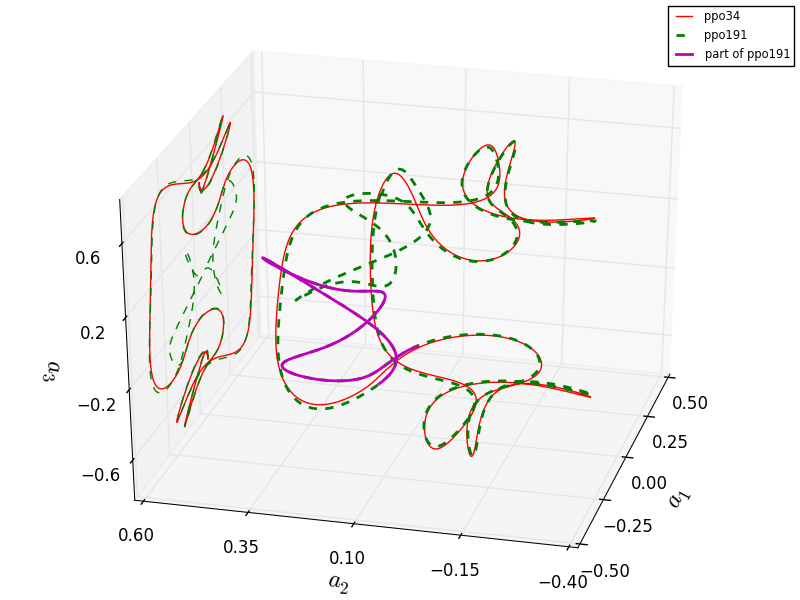
\includegraphics[width=1.0\textwidth]{ppo34ppo191.png}
	    \caption{
The orbit \cycle{ppo34} and \cycle{ppo191}. The purple part is a part of
\cycle{ppo191}, which I suspect has a \po\ close to it. The figure in
plane $a_{2}=0.8$ is  	a projection of the 3D figure.
	    }
	    \label{fig:ppo34ppo191}
    \end{figure}

    \begin{figure}[h]
    \centering
	    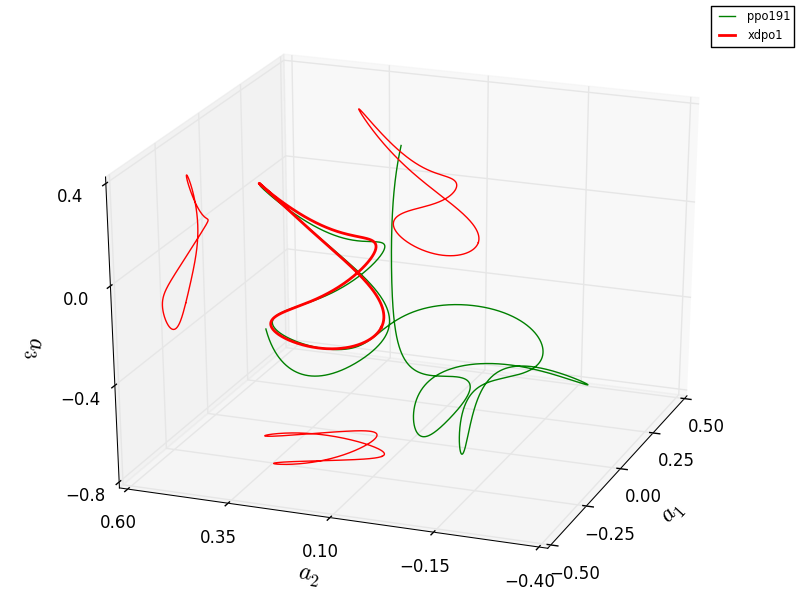
\includegraphics[width=1.0\textwidth]{xdpo1ppo191.png}
	    \caption{
The new \po\ \cycle{xdpo1} found by \LMa\ and its projection onto three
Fourier mode $[\ssp_i,\ssp_j]$ planes. The blue curve is a part of orbit
\cycle{ppo191}, which is used here to show the shadowing of these two
orbit.
	    }
	    \label{fig:xdpo1ppo191}
    \end{figure}


The initial condition for \cycle{xdpo1} is recorded in file \\
\texttt{siminos/xiong/matlab/data/xdks22ppo\_ve.mat},
which also contains the Floquet exponents and {\cLvs} for these orbits.
I have posted three videos to show the dynamics of these three orbits:
the 1st and 2nd Floquet vectors of
the pre-periodic orbit \cycle{ppo34}
\YTlink{www.youtube.com/watch?v=_7GYSWUhjU0}
\Xiong{2014-01-30}{Kazz: just to comment, I cannot play these Youtube videos... it just says "error".}
the pre-periodic orbit \cycle{ppo191}
\YTlink{www.youtube.com/watch?v=HSwF4FHcKP8},
and of
my first new \KS\ \po\
\cycle{xdpo1}
\YTlink{www.youtube.com/watch?v=KsKJlqanhzI}.
Click on the little gear, lower edge of the video, and increase
the resolution.

	\begin{table}[h]\small
	        \centering
                \rowcolors{1}{green}{pink}
                \begin{tabular}{ | c | c| c| c |}
		\hline
		   &  \large{\cycle{ppo34}}  	   &\large{\cycle{ppo191}} 	      & \large{\cycle{xdpo1}}       \\
		$\period{p}$ &  65.168     & 95.622		      &  28.661			 \\
		1  &  0.0906415303143404   & 0.163519387385378        &  0.310946570410124    \\
		2  &  7.6807244834054e-13  & -8.87742735450937e-10    &  1.82695233692736e-08 \\
		3  &  -3.96234572385144e-08& -2.92395682922365e-08    &  -1.00208509640834e-08      \\
		4  &  -0.0310548938604484  & -0.0880662661179373      &  -0.121543448733821         \\
		5  &  -0.179258937912979   & -0.153663430732254       &  -0.201501379498644         \\
		6  &  -0.256774704335013   & -0.288439007830585       &  -0.292650836258473   \\
		7  &  -0.27734427136977    & -0.297070591590133       &  -1.343131346286978   \\
                8  &  -0.32029818451026    & -0.324769085942675       &  -0.343131346286978  \\
              \end{tabular}
	      \caption{
Real parts of Floquet exponents for pre-\po s \cycle{ppo34},
\cycle{ppo191} and the \po\ \cycle{xdpo1}. For \cycle{ppo34} and
\cycle{ppo191}, period refers to the prime period. As \cycle{xdpo1} is
not self-dual under reflection, its prime period is the the whole period.	
	      }
	      \label{tab:floquet_exponents_ppo34ppo191xdpo1}
	\end{table}

\refTab{tab:floquet_exponents_ppo34ppo191xdpo1} gives the periods of
these three orbits and their Floquet exponents. The marginal exponents
are much more accurate than my in previous calculations because the
initial conditions for these orbits are refined by \LMa. As the two
shorter orbits shadow the longer one, the leading Floquet multiplier of
the long orbit is approximately a product of the Floquet multipliers of
the two shorter ones, so we expect:
	\begin{equation}
		\period{l}\,\eigRe[l]
         \approx \period{s1}\,\eigRe[s1]+\period{s2}\,\eigRe[s2]
    \,,
	\label{eq:relationorbits}
	\end{equation}
where $\eigRe[i]$ are the real parts of Floquet exponents. I checked this
relation for the first exponent, and I find the relative error is just
around 5\% ; therefore, we can predict the largest Floquet exponent of a
\po\ if we can find two or more shorter \po s to shadow it, which is
practically useful because calculating Floquet exponents is expensive
for long orbits.

However, relation \refeq{eq:relationorbits} is not satisfied by
other Floquet exponents
\Xiong{2014-01-30}{Kazz: I found it a sound and interesting observation.}.


\subsection{Very short time Lyapunov exponents}

Pre-\po s \cycle{ppo34} and \cycle{ppo191} are self-dual under reflection
symmetry, while orbit \cycle{xdpo1} maps into its twin.
\refTab{tab:floquet_exponents_ppo34ppo191xdpo1} shows that \cycle{xdpo1}
has two marginal exponents, one for perturbations along the orbit, and
the other for the \SOn{2} perturbations in the group tangent direction;
the continuous symmetry sweeps out a torus of \po s (not \rpo s).

\begin{description}

\item[2014-01-10 Xiong Ding]
{Video} \YTlink{www.youtube.com/watch?v=KsKJlqanhzI}
shows
that the local Floquet exponents for the 1st and 2nd {\cLvs}
repeat twice in one period. Therefore it should have some ``reflection''
symmetry. Am I right?

\item[2014-01-12 Predrag] Not if this is a pair of \po s related by
the reflection.
But I remember from \refref{Christiansen97} that the remanent of the $\SOn{2}$
circular group orbit restricted to the anti-symmetric subspace are two
points related by $\Zn{2}$. This might be the source of this reflection
symmetry. Presumably once you learn how
to slice and also quotient the discrete symmetry $\mathbf{Z}_2$, these will
be half period and much less wiggly.

\item[2014-01-12 Predrag]  What `local Floquet exponent' might be?
Eigen-exponent of a finite time Jacobian multiplier? That has no
meaning...

\item[2014-01-13 Xiong to Predrag] I am sorry the misleading term I created.
 I got the eigenvectors of Jacobian
matrix ({\cLvs}) and evolved them along the orbit. The logarithm of
expansion rates of {\cLvs} are recorded:

\begin{equation}
  \label{eq:locallyapunov}
  \lambda^{(i)}(t)=\frac{1}{h}\ln \frac{|v^{(i)}(t+h)|}{|v^{(i)}(t)|}
\,,
\end{equation}
where $h$ is the time step and index $i$ refers to the $i_{th}$ {\cLv}.
So, it should be the `local Lyapunov exponent'. Right?

\item[2014-01-13 Predrag] It looks like you are computing an arbitrary,
\emph{very} short time finite time Lyapunov exponent. Why would one do
that? This has no invariant meaning. It makes no sense at all to me. You
might just as well plot the eigenvalues of $\Mvar + \transp{\Mvar}$ as
function of $\ssp(\zeit)$, which is s symmetrized generalization of the
1\dmn\ derivative $\partial_x \vel(x)$ to higher dimensions. Would be
more useful to plot something like the angles $\cos(\theta_{ij}(\zeit))$
between Floquet eigenvectors $\{\jEigvec[i], \jEigvec[j]\}$.

Write up the definition of the finite time Lyapunov exponents, if you
have not done it yet someplace earlier in your blog notes. You can clip
\&\ paste the definition from
\\
\texttt{dasbuch/book/chapter/Lyapunov.tex}:
If the
unit vector $\unitVec$, $\norm{\unitVec} =1$ at the initial time
is aligned along the $i$th {principal stretch},
\(
\unitVec = {u}^{(i)}
\,,
\)
then the corresponding finite-time
Lyapunov exponent (rate of stretching) is given by
\beq
\Lyap_j(\xInit;\zeit) =
%\max_{\|\unitVec\|=1}
    \Lyap(\xInit,{u}^{(j)};\zeit)
    = \frac{1}{\zeit}\ln\sigma_j(\xInit;\zeit)
\,.
\ee{e:ftLyapStretch}
You would do me a great favor if you reread critically the Lyapunov
chapter in \textbf{ChaosBook.org}, edit/suggest improvements that would
make it easier to read :)

\item[2014-01-30 Kazz] Though I cannot say right now how such finite-time Lyapunov exponents can be used, I wouldn't say this is meaningless... This obviously gives local stretching rate of each Floquet vector. Therefore, I actually think that Xiong's speculation is correct... non? By the way, Xiong, you can directly check it simply by looking at the vector at time 0 and at a half of the period.


\end{description}

\subsection{Hyperbolicity of Floquet vectors}

According to Kazumasa~\etal\ previous work, hyperbolicity properties of
{\cLvs} have been used to
distinguish between the subspace of `{\entangled} Lyapunov modes' and
the subspace of contracting `{\transient} Lyapunov modes'. Their crucial observation
is that the {\transient} Lyapunov modes are nearly perpendicular to {\entangled} modes
and nearly perpendicular among themselves; however, the {\entangled} modes can be
tangential among themselves at some points. This observation indicates that
perturbations in the contracting {\transient} subspace  die out
 without any effect on
other modes.
But, since we can calculate the eigenvectors of Jacobian matrix, do Floquet
vectors have the similar properties as Lyapunov modes%
    \PC{I feel intense headache coming on - we talked about it on Friday
    and I thought we agreed. `Lyapunov modes' as used by Kazumasa and
    Hugues (I cite their definition in ChaosBook) is the set of both
    {\cLvs} and associated Lyapunov exponents of a given infinite time
    orbit, taken together. You have shown me that you have checked that
    for a \po\ the infinite time Lyapunov exponents do converge to
    $\eigRe[j]$, the real parts of Floquet exponents (evaluated on a
    single period), and you said were going to write that up (including
    the explanation that for complex pairs only the sum converges to
    $\eigRe[j]$, while each one singly oscillates with $\eigIm[j]$).  The
    only difference is that `Lyapunov' calculation converges only in an awkward and
    unnatural limit, convenient only for Oseledec rigorous mathematics, while
    Floquet is the natural object in dynamics.

    So what ``similar properties?'' For a \po\ `Lyapunov mode'
    \underline{is} identically the Floquet vector + the real part of the
    Floquet exponent, $[\jEigvec[j],\eigRe[j]]$.
    }
when applied to periodic orbits?

\begin{figure}[h]
  \centering
  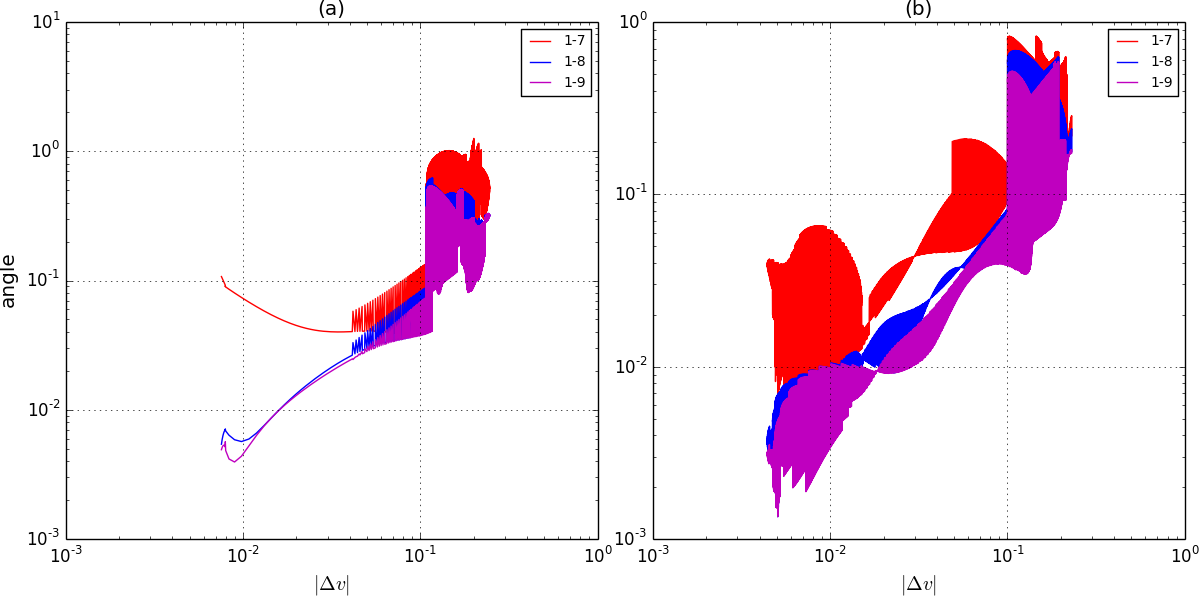
\includegraphics[width=1.0\textwidth]{ang789.png}
  \caption{The angle between the difference vector
  \refeq{eq:differencevector} and the subspace spanned by the first few
  Floquet vectors as a function of the Euclidean length $\norm{\Delta
  u(\zeit)}$ of the difference vector. (a) In the intervals where the
  pre-periodic orbit \cycle{ppo191} approaches \cycle{ppo34}, the first 7
  Floquet vectors are insufficient, but the first 8 Floquet vectors
  span the space that contains Delta $u(\zeit)$ to a good accuracy. (b)
  Pre-periodic orbit \cycle{ppo191} approaches \cycle{xdpo1}.
  }
  \label{fig:ang789}
\end{figure}

I take the re-periodic orbit \cycle{ppo191} together with \cycle{ppo34} and \cycle{xdpo1}
which shadow it. The difference vector is defined
as
\begin{equation}
  \label{eq:differencevector}
  \Delta u(\zeit)=u_{p_1}(t)-u_{p_2}(t-\tau)
\end{equation}
where, $u_{p_1}(t)$ and $u_{p_2}(t-\tau)$ are \statesp\ locations  of
 \cycle{ppo191} and \cycle{ppo34}( or \cycle{xdpo1}) respectively, and
parameter $\tau$ is chosen to minimize the Euclidean norm $\norm{\Delta u(t)}$.

If subspace spanned by `{\transient} Floquet modes' is disentangled from the
subspace spanned by `{\entangled} Floquet modes', then any perturbation along
the {\transient} Floquet modes will die out soon because its large negative
Floquet exponents; therefore, the difference vector should be within the
subspace of `{\entangled} Floquet modes'.

\begin{figure}%[h]
  \centering
  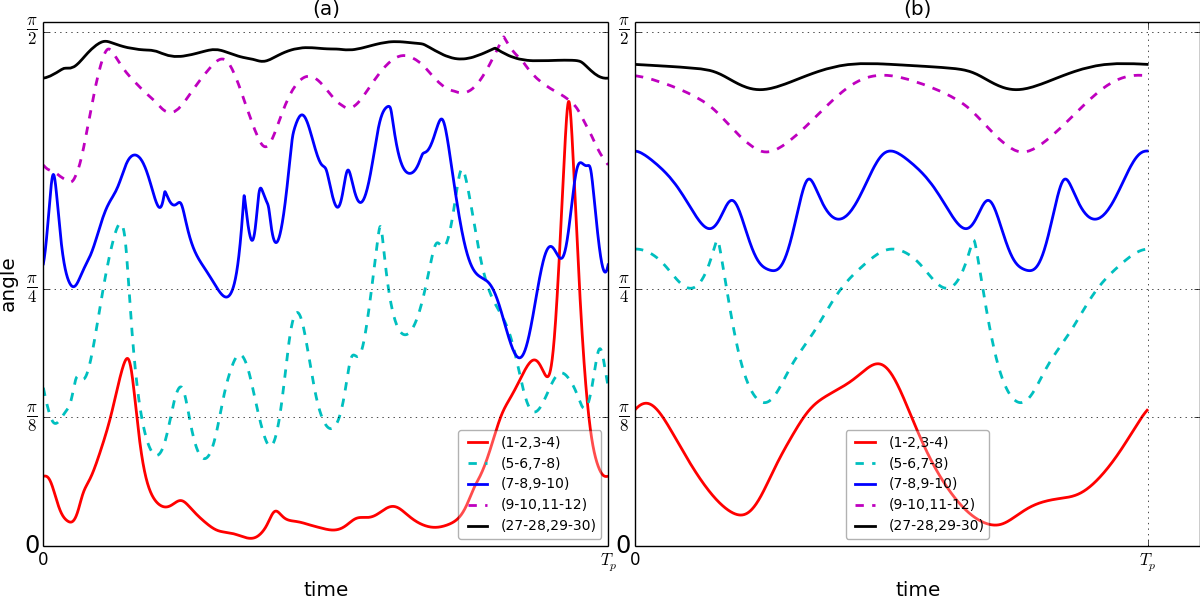
\includegraphics[width=1.0\textwidth]{angle_subspace.png}
  \caption{
  Smallest principal angles between subspaces spanned by Floquet vectors.
  (a) Pre-periodic orbit \cycle{ppo34}. (b) \po\ \cycle{xdpo1}
  }
  \label{fig:angle_subspace}
\end{figure}

\refFig{fig:ang789} shows the angle between the difference vector and
the hyperplane spanned by the first $N$ Floquet vectors for two pairs
of orbits.
    \PC{angle in what units? Degrees? Radians? If you plot $\sin$ of the
    angle instead, you do not have to say. Do you define this angle
    anywhere? Floquet vectors of which \po? Is the result similar for either?}
When $N=7$, the angle grows when the difference vector becomes shorter,
which indicates that the first 7 Floquet vectors cannot span the
{\entangled} subspace. However, when $N=8$ or $N=9$, the angle decreases
exponentially
\Xiong{2014-01-30}{Kazz: not exponential, but linear (slope = 1), as expected for the angle here.} as the two pre-periodic orbits get closer, and the
difference between the $N=8$ and case with $N=9$ cases is small. So,
could we say the first 8 Floquet vectors span the {\entangled} subspace?
At least for these three particular orbits?
    \PC{I do not get the oscillations in the solid color regions, and I
    do not get  \reffig{fig:ang789} at all - what do these blobs mean?
    Isn't there a unique $\tau$ for each value of $t$, \ie, each point
    $u_{p_1}(t)$ on the \po\ $p_1$?}
    \Xiong{2014-01-30}{Kazz: excellent! I agree about your conclusion here (and this number 8 is what we would expect from the physical dimension for ergodic trajectories!), though it's true that the blobs Predrag pointed out are worrying and we have to figure out what they are (and whether the result here is reliable). The definition of the \entangled subspace is not clear. Shall we \textit{define} the entangled subspace for a given pair of periodic orbits by the way you did here? I'd also like to see the fraction of time at which the two orbits are separated at each distance $|\delta v|$ in this figure. The averaged angle for small $|\delta v|$ must be obtained only from a few number of data (time steps), right?}

As we are interested in the intervals of small separations between nearby
orbits, perhaps the {\entangled} dimension can be detected by
investigating the neighborhood of a single periodic orbit. That is what
one does in the long time simulations of a single ergodic orbits; one
studies angles between its {\cLvs}, not its distances to other orbits or
it recurrences. \refFig{fig:angle_subspace} shows the angles between
different subspaces spanned by Floquet vectors for two of the shortest
periodic orbits of $L=22$ \KS.
        \PC{OK, angle is in radians. Do give a clear definition of the
        `principal angles'. Maybe plot $\sin$ on the logarithmic plot?}
While two \po s are insufficient to make a statistical analysis of small
angles, presumably what we care about are the minima along a given orbit,
as these are the instants where perturbation along one of the {\cLvs} is
most entangled. In these examples the leading {\cLvs} are most entangled,
while {\cLvs} beyond the 8th one are always quite orthogonal to the rest,
in agreement with the long-time simulations.

\begin{description}

\item[2014-01-30 Kazz] Excellent!! This is really what we wanted to see! However, it's too early to conclude that the physical dimension of ergodic trajectories can be estimated from a pair of periodic orbits: it may be just a coincidence! What we really have to do is to elucidate in what conditions the entangled subspace dimension of a given pair of periodic orbits gets equal to the phydical dimension. We (Hugues and I) speculate that hyperbolicity of periodic orbits matters. How hyperbolic are the two orbits you used here? In other words, what is the minimum angle between two entangled {\cLvs} (i.e. two of the first eight {\cLvs}) ? If these orbits are rather hyperbolic, try to find a pair of nearly non-hyperbolic orbits (or a pair of a hyperbolic orbit and a nearly non-hyperbolic one) and measure the same thing. What do you get?



\item[Xiong Ding 2014-04-15]

  \begin{figure}[h]
    \centering
    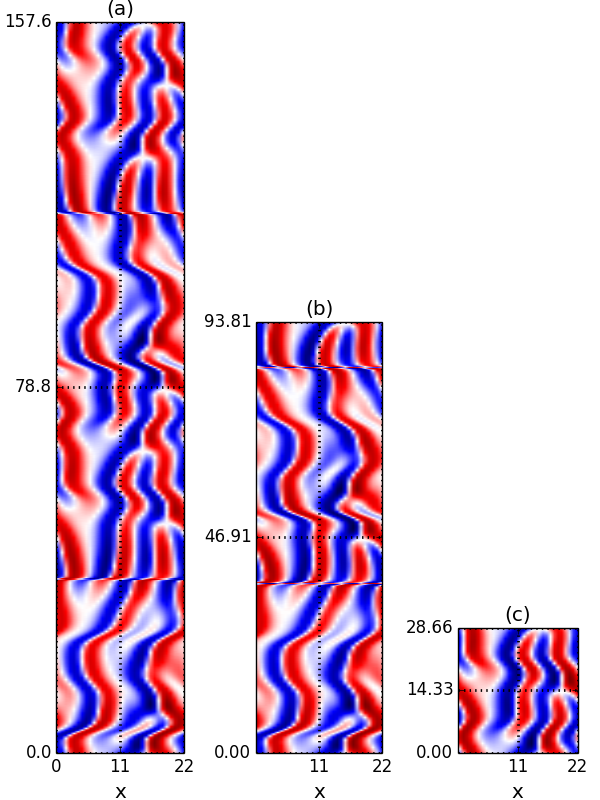
\includegraphics[width=0.8\textwidth]{state69_13_2_SO2fm1}
    \caption{State space onfiguration of (a) \cycle{ppo69}, (b)
      \cycle{ppo13} and (c)
      \cycle{ppo2} after quotienting out \SOn{2}\ symmetry by the first
      Fourier mode slicing. All of them are evolved for $2T_{p}$ with $T_{p}$
      the prime period respectively.
    }
    \label{fig:state69_13_2_SO2fm1}
  \end{figure}

I repeated the same procedure as above on another pair of shadowing orbits: \cycle{ppo13} and \cycle{ppo69}. Two cases are considered here depended
on the different definitions of difference vector, one of which does not
consider \SOn{2}\ symmetry while the other does.

\paragraph{The first case}
In this case, difference vector is defined as
$\Delta u(t_1)= u_{p_1}(t_1)-u_{p_2}(t_2)$ with $t_2$ minimizes the
Euclidean norm of $\Delta u(t_1)$.

\begin{figure}[h]
  \centering
  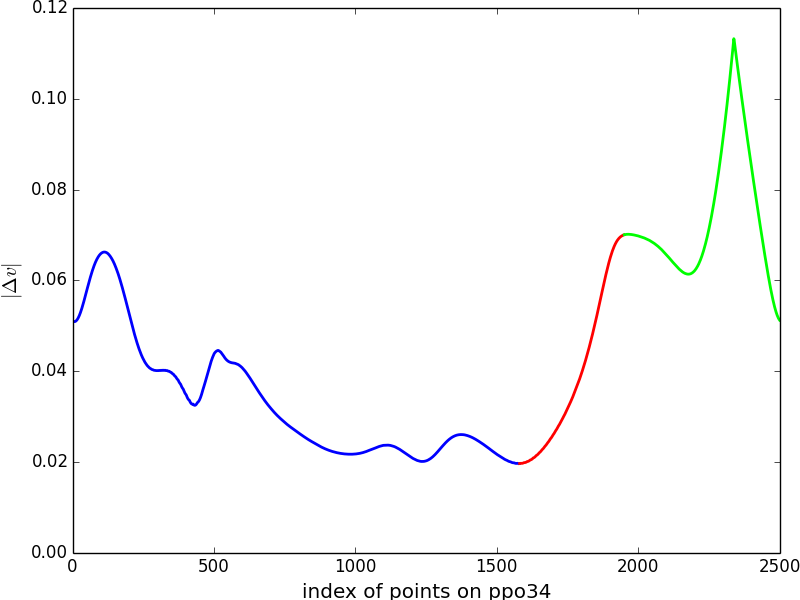
\includegraphics[width=1.0\textwidth]{dis_69_13}
  \caption{Euclidean norm of the difference vector along \cycle{ppo13}.
    Red and blue lines represent the part when the two
    orbits(\cycle{ppo13} and \cycle{ppo69}) shadow each other,
    and green curve represents the part at which these two orbits diverge
    from each other. The red part is chosen as the incidence window.
    In this plot \SOn{2}\ symmetry has not been considered.
  }
  \label{fig:dis_69_13}
\end{figure}

\begin{figure}[h]
  \centering
  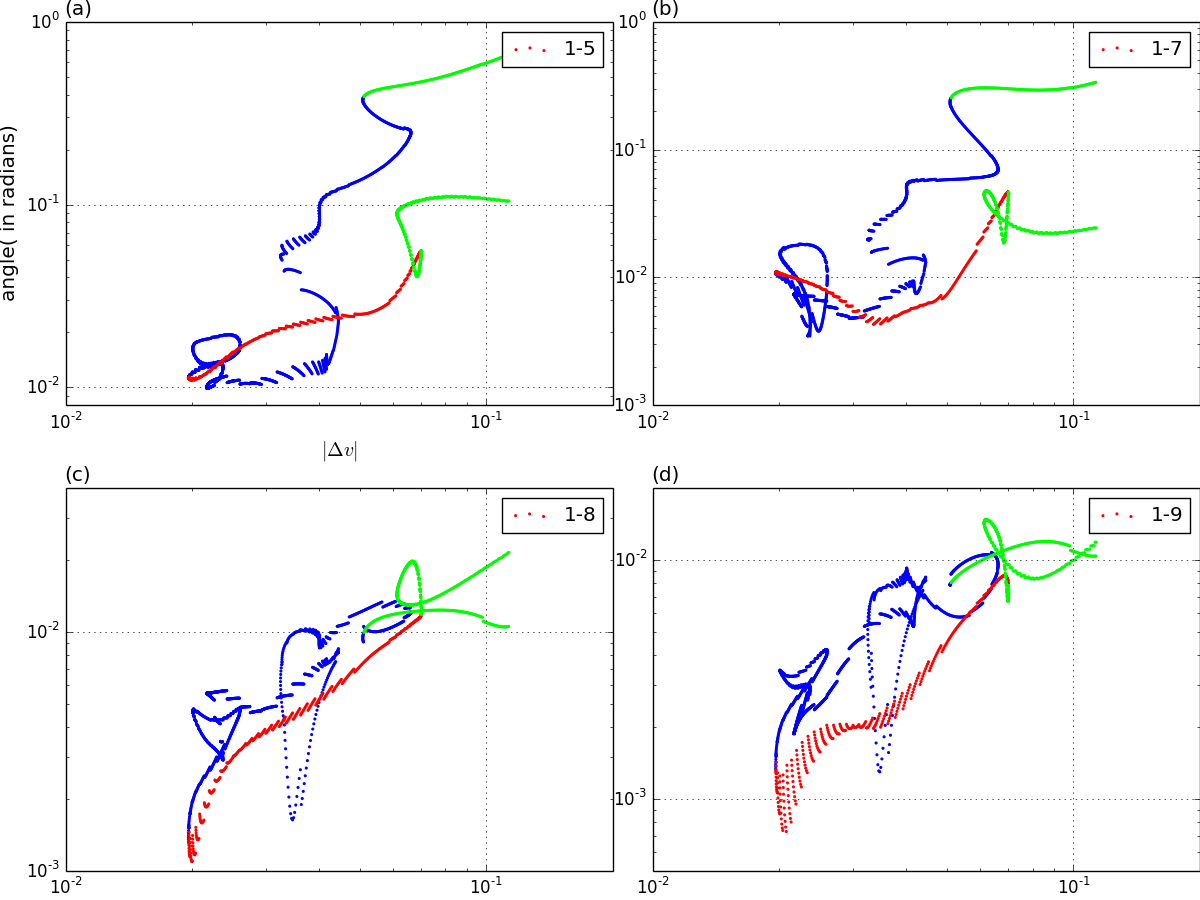
\includegraphics[width=1.0\textwidth]{dis_ang_69_13}
  \caption{
    Angle between difference vector and the subspace spanned by
    the first few Floquet vectors. Orbit $p_2$ approaches orbit
    $p_1$. First few Floquet vectors
    of orbit $p_1$ are used to span the subspace. In this
    case, $p_2$ is \cycle{ppo69} and $p_1$ is \cycle{ppo13}.
    (a) (b) (c) and (d) use 5,7,8 and 9 first Floquet vectors
    respectively to span the subspace. Red, green and blue dots
    correspond to the same part of incidence in \reffig{fig:dis_69_13}. In this plot \SOn{2}\ symmetry has not been
    considered.
    The discontinuity in the plot does not come from
    code error. When trying to
    find difference vectors, the distance is minimized, so the
    direction of difference vector may changed a little abruptly
    at some moment, especially when the distance is really small.
  }
  \label{fig:dis_ang_69_13}
\end{figure}

\paragraph{The second case} \SOn{2}\ symmetry is taken into account.
The definition of difference vector is
\beq
\Delta u(t_1)= u_{p_1}(t_1)-g(\theta)u_{p_2}(t_2)
\,,
\ee{eq:difvec_SO2}
where $\theta$ and $t_2$ are chosen to minimize the Euclidean
length of $\Delta u(t_1)$. Here $g(\theta)$ is an \SOn{2}\ group transformation
and $p_1,p_2$ are two periodic orbits. In our case, $p_1$ is \cycle{ppo13}
and $p_2$ is \cycle{ppo69}.

I have read \refsect{sect:DraftBlog}, about the debate
between Evangelos and Kazz on the issue of determining
optimal shift when defining the difference vector.
It seems that Kazz tried to align the second Fourier
modes of a ergodic trajectory and a periodic orbit, so
he thought his route is approximate. As pointed out by him
(2011-08-11 Kazz 2 Evangelos), the reason he did not use the definition
\eqref{eq:difvec_SO2} is a pure computational issue: this definition
is very expensive numerically. I sincerely sympathize with him because
I encountered the same problem at the beginning.  Everyone including me
believes that if the optimal shift is determined between two points, then
Newton method will easily generate all the optimal shifts between other
points because the flow is continuous and the only variable is the group
angle $\theta$ , but actually the situation is
more complicated than we thought because we cannot predict which local
minimal point the Newton method will converge to. For example,
at point $x(t)$, take $\theta_1(t)$ and $\theta_2(t)$ as the two local
optimal shifts and $\theta_1(t)$
is also the global minimal. The Newton method converges
to $\theta_1(t)$, which is good. We now use $\theta_1(t)$ as the initial
condition to computer the optimal shift at next step $x(t+dt)$, and
Newton method probably converges to $\theta_{1}(t+dt)$; however, we could
not claim that $\theta_{1}(t+dt)$ is the global optimal shift because
$\theta_{2}(t+dt)$ may generate smaller Euclidean distance between the
two new points. What's more, I cannot find a way to predict when this
situation will happen. Initially, I wrote a Matlab script to implement
\eqref{eq:difvec_SO2}, but gave up soon because I lost my patience.
Finally, I turned to C with optimization and parallelization. Now it
is tolerable at least for short orbits (trajectories).

I hope I understand the \refsect{sect:DraftBlog} discussion correctly.

\begin{figure}[h]
  \centering
  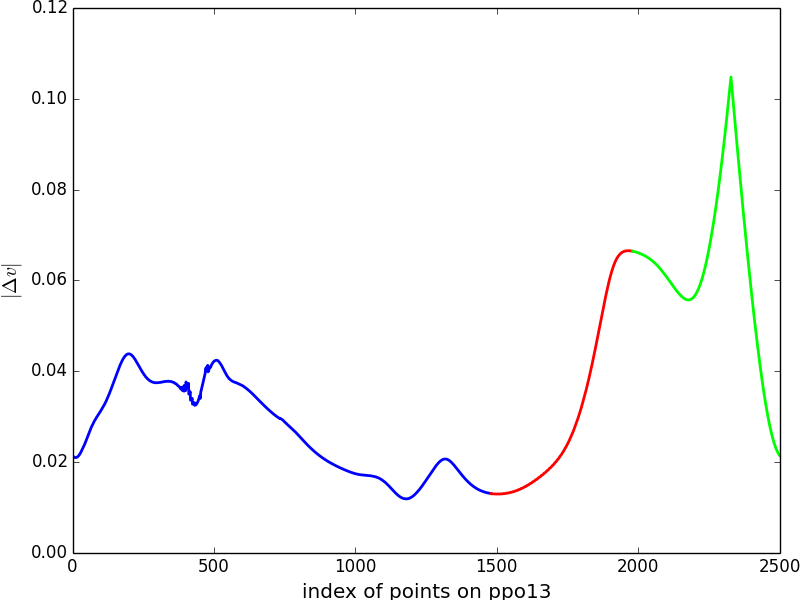
\includegraphics[width=1.0\textwidth]{dis_69_13_SO2}
  \caption{Norm of the difference vector along \cycle{ppo13}.
    Red and blue lines represent the part when the two
    orbits(\cycle{ppo13} and \cycle{69}) shadow each other,
    and green curve represents the part at which these two orbits diverge
    from each other. The red part is chosen as the incidence window.
    In this plot \SOn{2}\ symmetry has been considered.
  }
  \label{fig:dis_69_13_SO2}
\end{figure}

\begin{figure}[h]
  \centering
  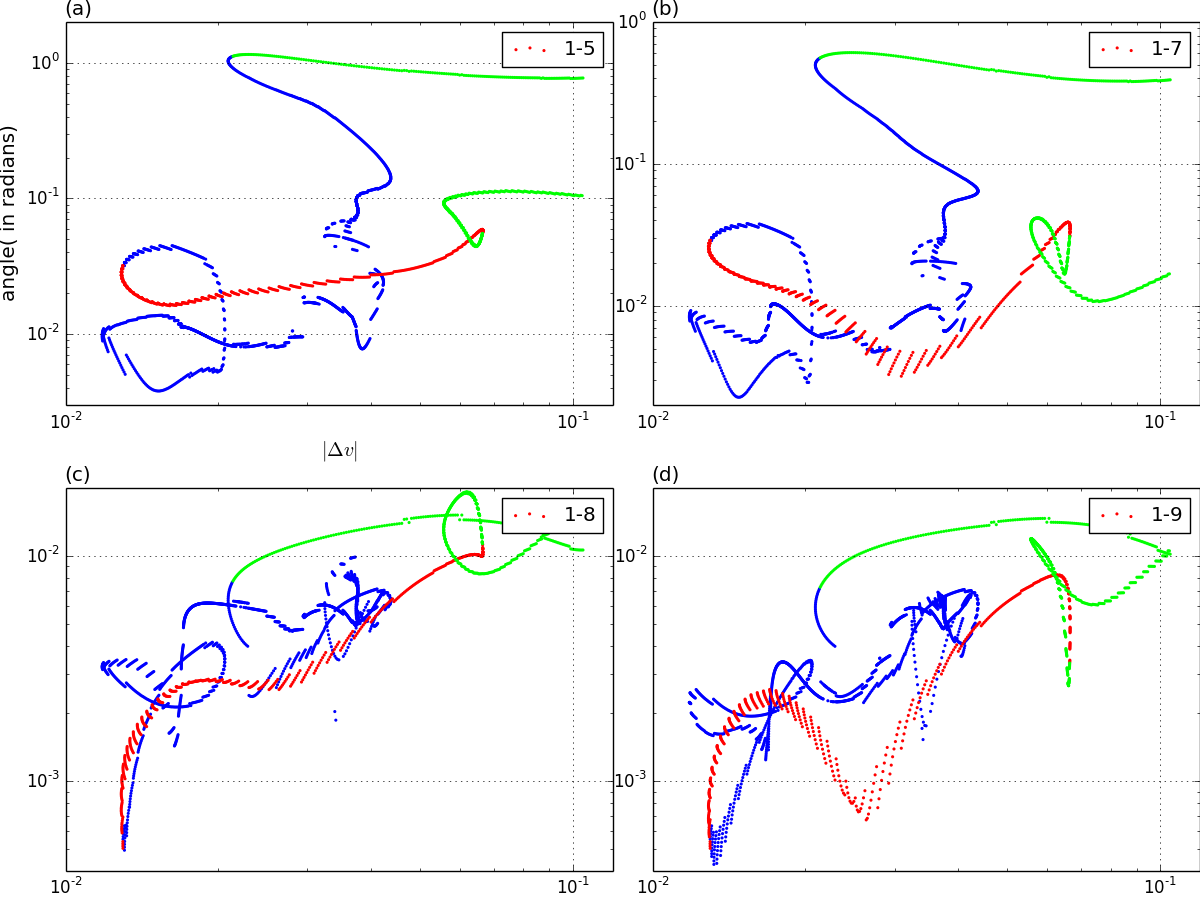
\includegraphics[width=1.0\textwidth]{dis_ang_69_13_SO2}
  \caption{
    Angle between difference vector and the subspace spanned by
    the first few Floquet vectors. Orbit $p_2$ approaches orbit
    $p_1$. First few Floquet vectors
    of orbit $p_1$ are used to span the subspace. In this
    case, $p_2$ is \cycle{ppo69} and $p_1$ is \cycle{ppo13}.
    (a) (b) (c) and (d) use 5,7,8 and 9 first Floquet vectors
    respectively to span the subspace. Red, green and blue dots
    correspond to the same part of incidence in
    \reffig{fig:dis_69_13_SO2}. In this plot \SOn{2}\ symmetry has been
    considered.
  }
  \label{fig:dis_ang_69_13_SO2}
\end{figure}

\clearpage
\subsection{Statistical results}

For two subspaces $\mathcal{F}\in\pS$, $\mathcal{G}\in\pS$ of a space
$\pS$ equipped with an inner product, the principal angles (canonical
angles) $\theta_k$ between vectors $u\in \mathcal{F}\,, v\in \mathcal{G}$,
\[
\cos(\theta_k) = \max
u^\top v = u_k^\top v_k
\,,
\]
subject to restriction
\[
||u|| = ||v||=1\,, u^\top u_i = 0\,, v^\top v_i = 0\,, i = 1,\cdots,k-1
\,,
\]
provide information about the relative position of $\mathcal{F}$ and
$\mathcal{G}$ inside the full space\rf{Knyazev02}.
The number of principal angles is
$q = \min(\dim\mathcal{F}, \dim\mathcal{G})$,
and the smallest one is the smallest angle that can be spanned by two
arbitrary vectors, one from each subspace. For example, for two perpendicular
planes inside a 3d space, the two principal angles are $0$ and
$\pi/2$.  On the other hand, if one subspace is one-dimensional, then
the unique principal angle refers to the projection angle of a vector
to a subspace. Knyazev and Argentati\rf{Knyazev02} give a simple algorithm
to calculate
principal angles,
\[
\theta_k = \arccos(\sigma_k)\;, k = 1,2,\cdots, q
\,,
\]
with
\[
svd(Q_F^\top Q_G) = diag(\sigma_1, \cdots, \sigma_q)
\,,
\]
where $svd$ refers to singular value decomposition. $Q_{F}$ and $Q_G$ are
orthonormal basis inside each subspace. Numerically, the algorithm can
be implemented as a singular value decomposition after two QR
decompositions.

In order to distinguish the disentangled and entangled subspace in \KSe,
the general idea is to determine the likelihood of random
small perturbation in one subspace evolving into the other
subspace as time goes on. \refRef{YaTaGiChRa08} uses CLVs to investigate
the embedding dimension of the global attractor of KS system; here,
on the other hand, we turn to Floquet vectors associated
with periodic orbits since they govern the dynamics inside the
tangent space, so for our purpose, the obvious way is to study the smallest
principal angle between subspaces spanned by different combinations
of Floquet vectors along these orbits.

\cycle{ppo} and \cycle{rpo}, with periods $\period{p} < 100$, are used as samples in
 \reffig{fig:statistic_angle_rpoppo}. We put threshold index at $7, 8, 9$
and record the smallest principal angles along each orbit. When the 7th and
8th Floquet vectors form a complex conjugate pair, then the indices are
changed to $6, 8, 9$. The same goes for other indices.

We first observe
that 8th and 9th never form a conjugate pair, but other possibilities
occurs for some orbits. Also from (a) and (c) in
 \reffig{fig:statistic_angle_rpoppo}, we can see that
the angle mostly stays near zero when the 8th is separated
from the first seven Floquet vectors, but immediately exclude 8th from the
remaining subspace, the distribution shift to large angles, which means
that the first 8 dimensions are closely related to each other but are
quantitatively separated from the remaining dimensions. Also there is
a peak accumulation at larger angle for index equal to 8 and 9.
The angles between vectors are plotted in (b) and (d). The
angles for vectors inside the entangled zone have fairly flat distribution
from 0 to $\pi/2$, but angle between vectors from entangled and
disentangled space or both from disentangled space mainly accumulate
near $\pi/2$.

\begin{figure}[h]
  \centering
  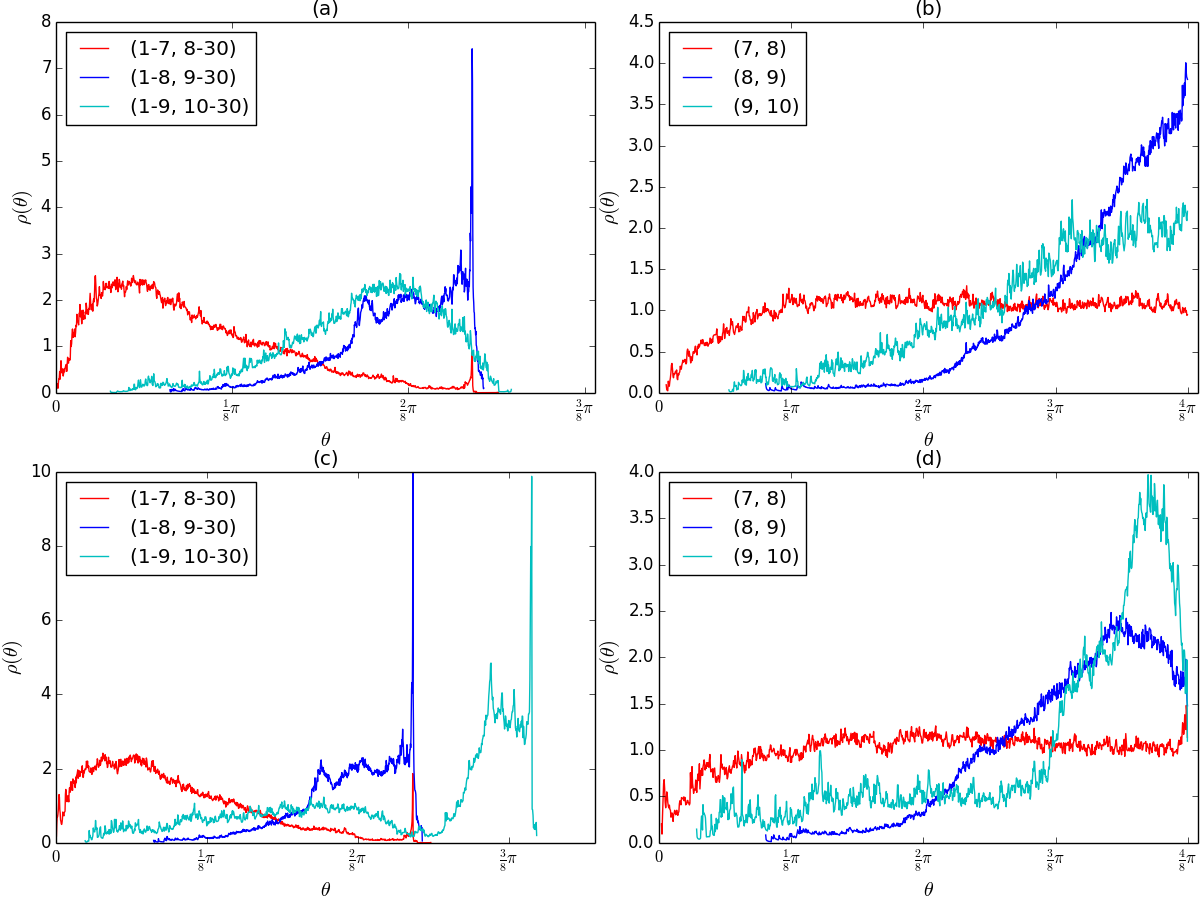
\includegraphics[width=1.0\textwidth]{statistic_angle_rpoppo}
  \caption{
    (a)(b) Smallest principal angle distribution for the first
    240 pre-periodic
    orbits ($T_p < 100$). Number in the parentheses donate the indices
    of Floquet vectors that span the corresponding subspace. $y$-axis
    is the normalized distribution, and $x$-axis is the span of angles.
    (c)(d) The same graph for the first 239 \rpo s with
    $T_p < 100$.
  }
  \label{fig:statistic_angle_rpoppo}
\end{figure}


Another way to investigate the local dimension of \KS\ system is to
find how good enough the first few Floquet vectors can expand the
difference vector which is defined as
\[
\Delta x = \hat{x}(t_p) -\hat{x}_0
\,,
\]
where the hat means the vector is defined in \SOn{2}\ reduced space
(for simplicity, we choose the first Fourier mode slice), and $t_p$
denotes the time to evolve the state onto the {\PoincSec} defined by
template point $\hat{x}_0$ and the velocity field at $\hat{x}_0$.

The definition used here eliminates the importance of the two marginal
vectors in the full spectrum of Floquet vectors associated with each
orbit. In order to find how many dimensions are needed to fairly expand
the difference vector, Floquet vectors are first projected onto the 1st
mode slice and then projected onto the {\PoincSec}. A detailed
description abofout this technique is given in \refsect{sect:symm}.
Ergodic trajectories are obtained in the full state space and then
reduced in the 1st mode slice, after which, {\PoincSec} points are
collected.

\begin{figure}[h]
  \centering
  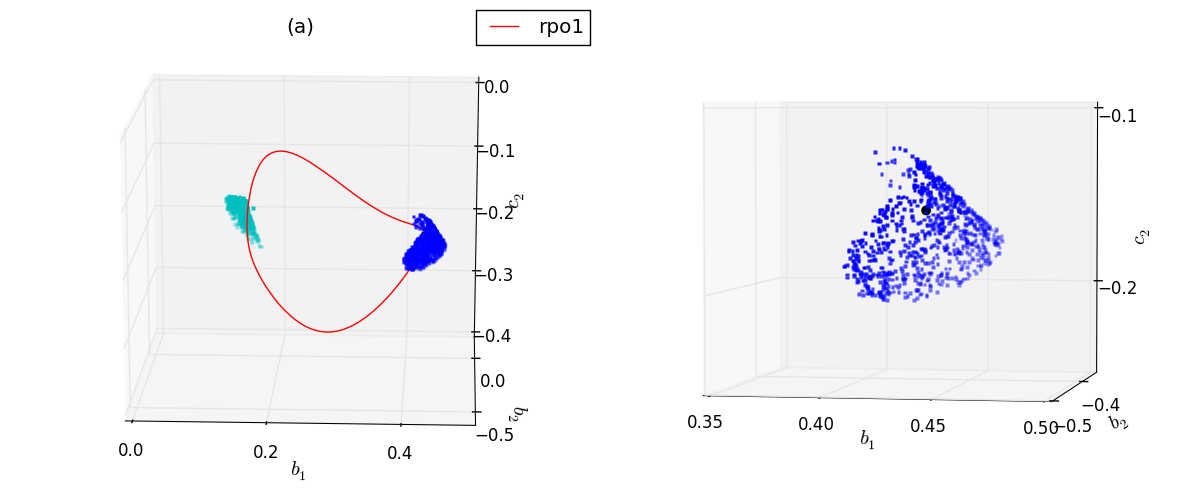
\includegraphics[width=1.0\textwidth]{poincare_intersection_rpo1}
  \caption{(a) \cycle{rpo1}(red) with the two sets of {\PoincSec s}
    (blue and cyan)
    points near the border and far away from the slice border. The points
    are generated from an arbitrary initial point on the attractor, and
    velocity field at the template point is used to define the {\PoincSec}. Only intersection points close enough to the template points
    are recorded. (b) the magnified version of the template point far away
    from the slice border (black point) and the intersection point around
    it (blue).
  }
  \label{fig:poincare_intersection_rpo1}
\end{figure}

\begin{figure}[h]
  \centering
  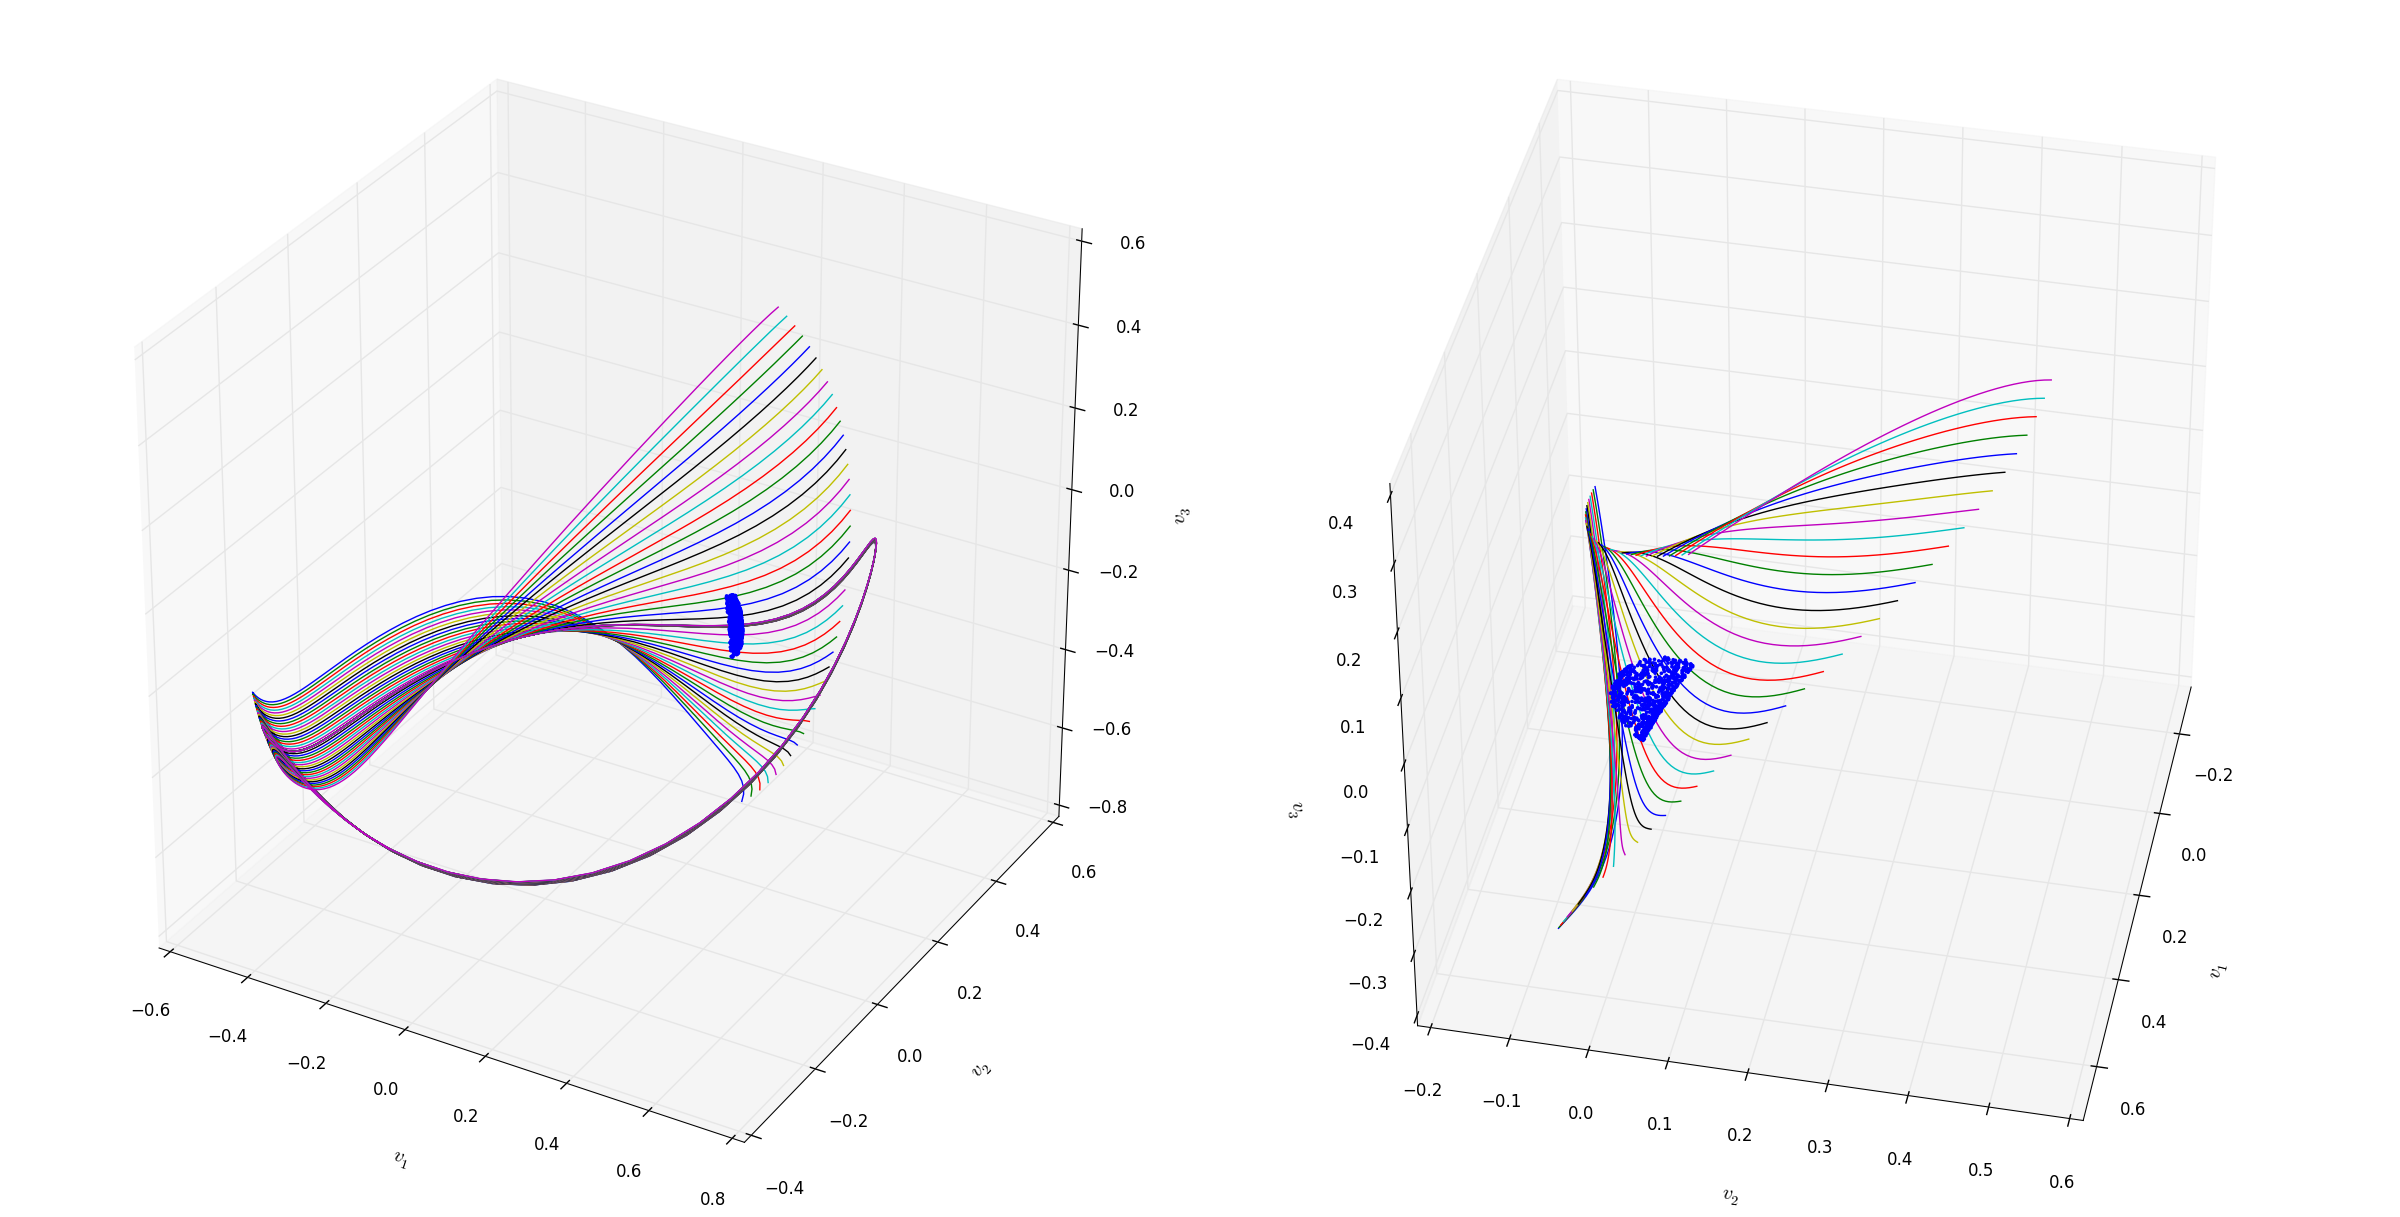
\includegraphics[width=1.0\textwidth]{manifold_rpo1}
  \caption{Unstable manifold of \cycle{rpo1} on the 1st mode slice. The
  axes $v_1$, $v_2$, $v_3$ are Floquet vectors $e_1$, $Im(e_5)$ and
  $Re(e_5)$. (b) is the same as (a) with a different angle of view.
}
  \label{fig:manifold_rpo1}
\end{figure}

We choose the farthest and closest point on an orbit as template point
to construct {\PoincSec} to demonstrated that \SOn{2} reduction will
not change the local structure in the full state space. On the other
hand, the velocity field at the two location are most likely parallel
to the slice border and thus the resulting {\PoincSec} is perpendicular
to the slice border. Our experience tells us that ergodic trajectories
tend to move around the slice border from time to time, so in this way,
we are more likely to get a lot of intersection points.

 \refFig{fig:poincare_intersection_rpo1} shows that when only 5 Floquet
vectors are used to span the subspace, the principal angle will not
diminish as we get closer to the template point, which means 5
dimensions are not enough to construct the local structure around the
template point. However, when one more Floquet vector is added, the
scenario changes immediately. As the distance decreases, the
corresponding principal angle decrease accordingly. Also, if more
dimensions are added, the scenario does not change qualitatively.
Therefore, we reach the conclusion that local dimension at these
template points is $6$ on the {\PoincSec} and 8 in the full state
space. Note that there is a distinct structure on the data collected.
It seems that the relation is linear, and the slope may indicate the
properties of the local structure, which are unknown to me. On the
other hand, the length of difference vectors ranges from 0.01 to 0.1
because of the extremely low probability to obtain intersection points
much closer to the template point along an ergodic trajectory. Maybe we
can get more convincing result if longer evolution time is employed.

\begin{figure}[h]
  \centering
  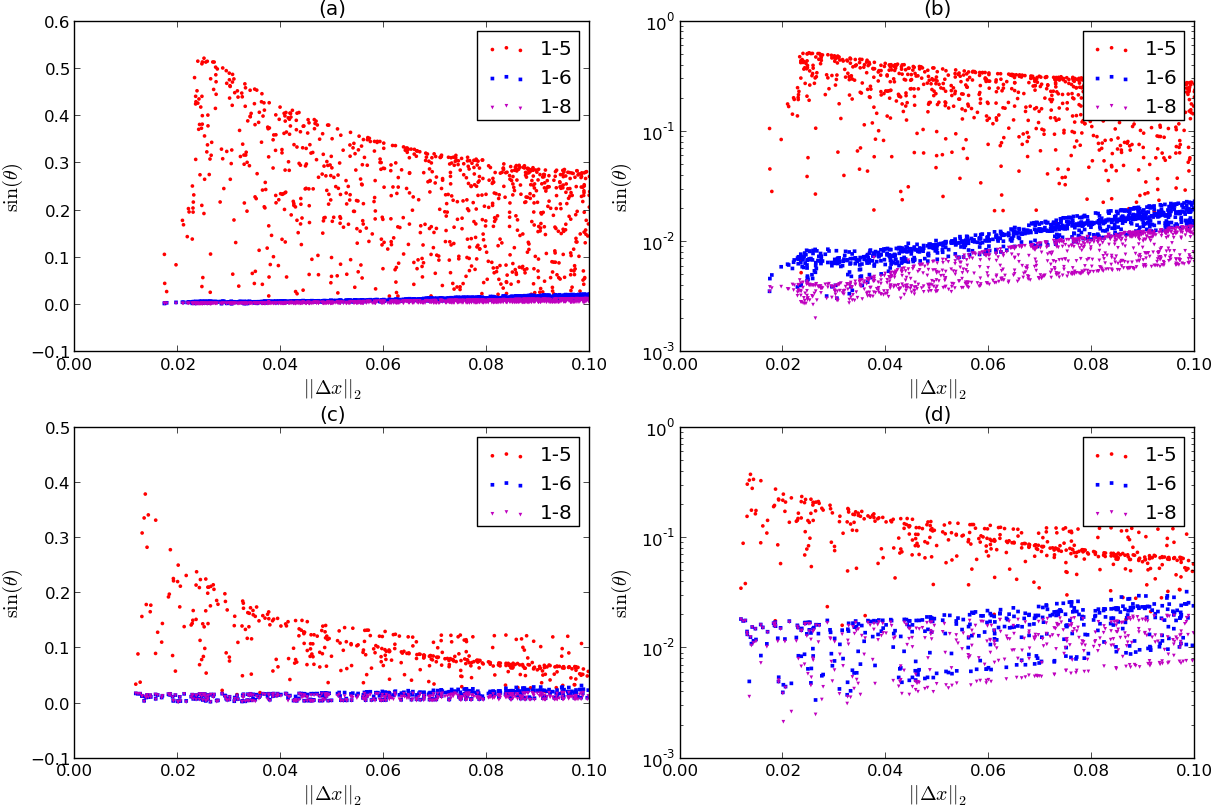
\includegraphics[width=1.0\textwidth]{ergodic_angle_rpo1}
  \caption{
    Principal angle between difference vector and subspace spanned by the
    first few Floquet vectors versus the Euclidean length of the difference
    vector. Difference vector is defined on the {\PoincSec} constructed
    from farthest/closet point on \cycle{rpo1} to slice border.
    The right side
    is the same figure as the left side with y-axis changed to log scale.
    The legend specifies how many Floquet vectors are used to construct
    the local subspace. Note the 7th and 8th Floquet vectors form a
    complex conjugate pair.
    (a) (b) Farthest point is chosen as the template point of {\PoincSec}. 885 points are collected.
    (c) (d) Nearest point is chosen as the template point of {\PoincSec}.  397 points are collected.
  }
  \label{fig:ergodic_dis_angle_rpo1}
\end{figure}

This experiment is conducted for other orbits.
\refFig{fig:ergodic_dis_angle2} shows similar results for several
other cycles. It clearly shows that the local dimension
is 8 for most state points. However, when I tried to do
the same experiment for \cycle{ppo4}, the result is different
from all the others as shown in figure. Although there is distinction
between the first 7 and 8 dimensions when expanding the difference
vector, the tendency of the movement of these intersecting
points is not along a
declining line when distance is getting smaller. I guess this
observation should indicate
a different local structure as was shown in
 \reffig{fig:ergodic_dis_angle2}.

\begin{figure}[h]
  \centering
  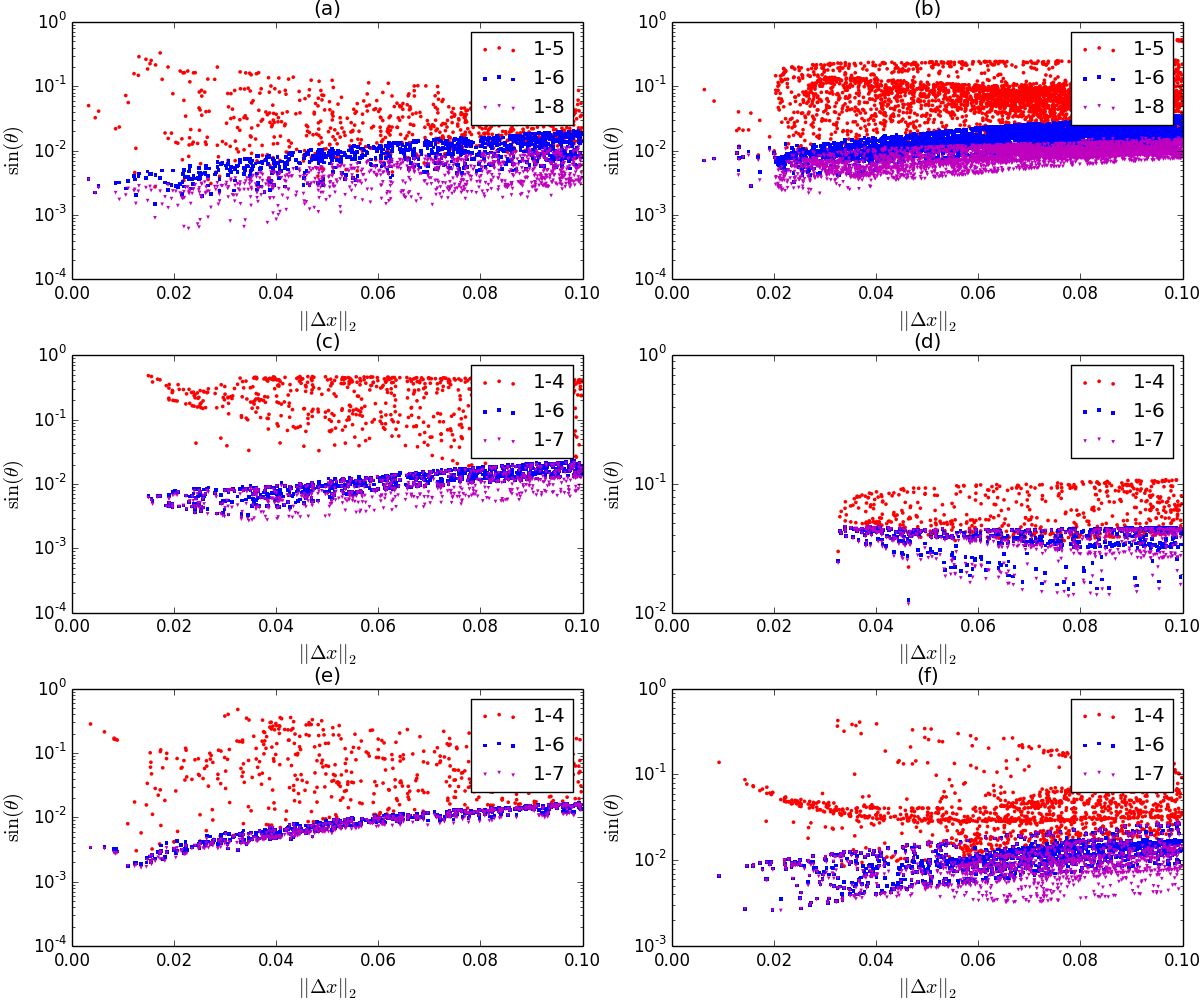
\includegraphics[width=1.0\textwidth]{ergodic_dis_angle2}
  \caption{
    The same experiment as \reffig{fig:ergodic_dis_angle_rpo1}.
    (a) (b) \cycle{rpo3} with {\Poincare} template point far away
    from slice border (left graph) and near the slice border
    (right graph).
    (c) (d) For \cycle{ppo2}.
    (e) (f) For \cycle{ppo9}
  }
  \label{fig:ergodic_dis_angle2}
\end{figure}

\begin{figure}[h]
  \centering
  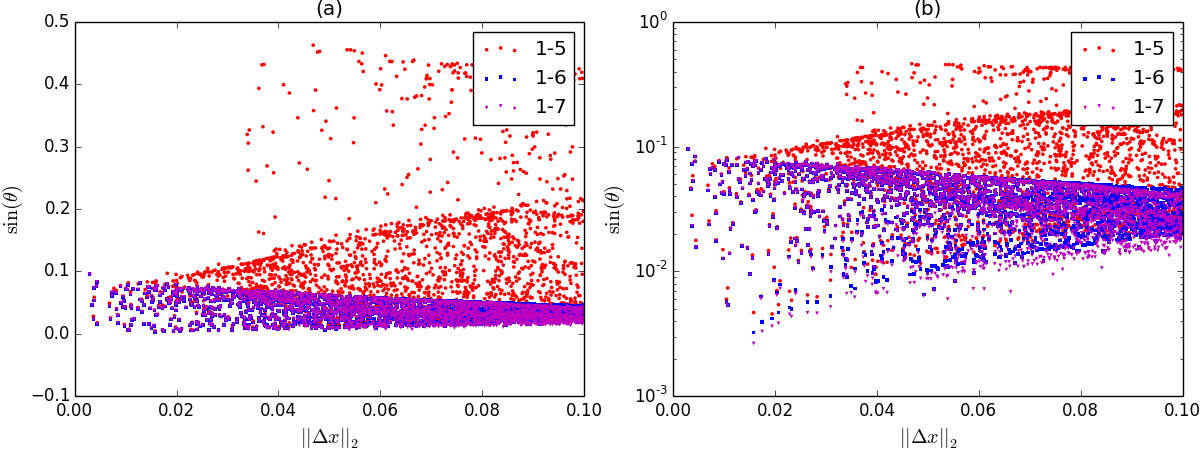
\includegraphics[width=1.0\textwidth]{ergodic_dis_angle_ppo4}
  \caption{
    The same experiment on \cycle{ppo4} as \reffig{fig:ergodic_dis_angle_rpo1} at the far side of slice border.
    (a) and (b) are the same
    experimental data with different schemes of y-axis scale.
   }
  \label{fig:ergodic_dis_angle_ppo4}
\end{figure}


\item[Predrag 2014-09-05]

Started taking notes from the WebEx meeting, cannot finish - someone
please take over with writing up the summary:

Hugues: do you get different plots if you separate statistics into
one real expanding eigenvector and the set of complex pair?

XD: there are very few orbits which are complex expanding pairs.
Expect similar statistics

Hugues: what is statistics of set of long orbits
(remove those shorter than - let's say 20)?

XD: will have a look

XD: blue and green curves are strictly bounded away from zero.

XD: we do not know why there are sharp peaks at larger angles?

PC: why is the green curve so different between \po s and \rpo s?

HC/KT: Has the peak in the blue curve physical meaning?

ES: is the peak in the blue (and red) curve at the same location for rpos and pos?

XD: Yes, almost the same location.

XD: I am worried about the results of \reffig{fig:ergodic_dis_angle_ppo4}.

HC: This ppo might be isolated from the attractor.

XD: However, the ergodic trajectory comes close to it.

ES: This has to do with how we measure distance. We always use Euclidean distance
but this cannot tell us if the orbit is on the attractor or not. We would neeed to
understand topology in order to answer this question, but this might be very hard.

ES: Maybe you could plot the intersection of the unstable manifold of
the orbit in \reffig{fig:ergodic_dis_angle_ppo4} with a {\PoincSec} and
the same for an ergodic orbit, and see if there is transverse distance
between them.

ES 2014-09-07: Also, at the points of closest approach of the trajectory and the ppo,
the velocities should not be misaligned if the latter is part of the attractor.

ES: (for next paper?) You could try to understand if the local dimension changes
along a long orbit that shadows two short orbits with different number of expanding
directions, \ie, produce a more sensible version of \reffig{fig:ks22shad} using
the smallest principal angle approach.

ES: {\PoincSec} is a bit confusing in 3D. Could you plot a 2D
projection, including points of intersection on the unstable manifold
of the rpo, rather than trajectories?

Everyone: We think there is now enough for a nice, short (max 4 pages) publication.
Kazz will produce the skeleton.

\item[Evangelos 2014-09-07] In order to understand what is going
on in \reffig{fig:ergodic_dis_angle_ppo4},
it might help to plot the data for the smallest principal angle for this orbit
and compare it to the data for a non-problematic orbit. There should be a difference
in how close the red curve comes to zero.

\item[Evangelos 2014-09-07] Actually \reffig{fig:ergodic_dis_angle_ppo4} might be
a way to tell if an orbit is part of the attractor or not.

\item[Xiong 2014-09-07] I tried to answer some of these questions.

\textbf{Blue and green curves are strictly bounded away from zero.}
this can be demonstrated by the y-log scale
\reffig{fig:statistic_angle_rpoppo_log}. Distribution $\rho(1/\theta)$
is not used here to show the boundedness because I did not get a good
exponential relation as
Kazumasa did in \refref{TaGiCh11}. One problem is panel (B):
the red line does not end on the y-axis. There is very small
gap. could we just account for it the shortage of data points?

\begin{figure}[h]
  \centering
  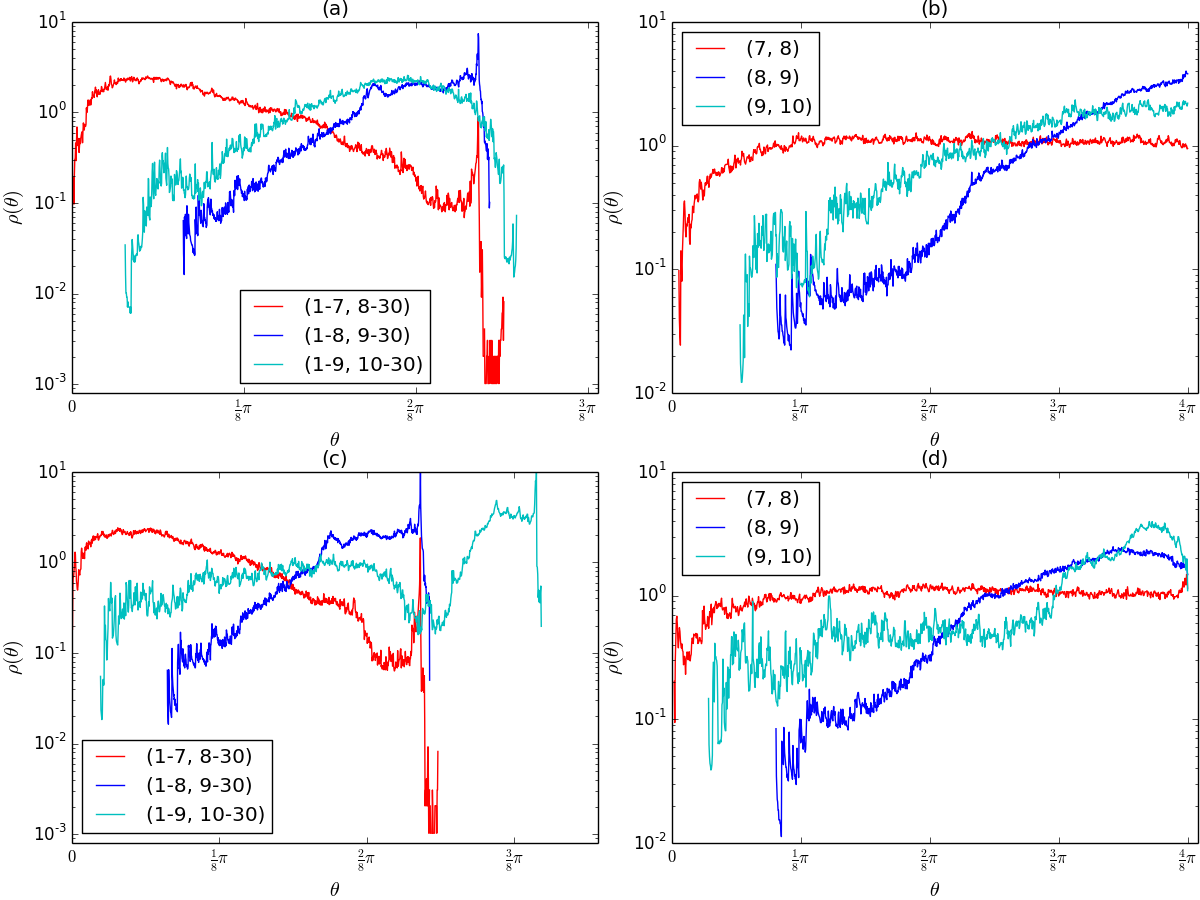
\includegraphics[width=1.0\textwidth]{statistic_angle_rpoppo_log}
  \caption{
  The same as in \reffig{fig:statistic_angle_rpoppo} but with log scale.}
  \label{fig:statistic_angle_rpoppo_log}
\end{figure}


\textbf{Do you get different plots if you separate statistics into
one real expanding eigenvector and the set of complex pair?} I presumed that
the orbits with two expanding directions (two real or complex conjugate)
are
far fewer than those with only one expanding direction; however it turns
out that I was wrong. Of the 240 pre-periodic orbits ($T<100$) and
239 relative periodic orbits, 167, respectively 159, have only
one expanding directions. So orbits with two expanding directions are about
one thirds of the total orbits with periods less than 100.
But the statistics
of these two types of orbits exhibit no striking difference as shown in
\reffig{fig:statistic_angle_rpoppo_AB}. Note that log scale is not used
because for curves oscillate strongly at the tails. Also number of bins in the
histogram \reffig{fig:statistic_angle_rpoppo_AB} is 400. For other figures,
1000 is used.
\begin{figure}[h]
  \centering
  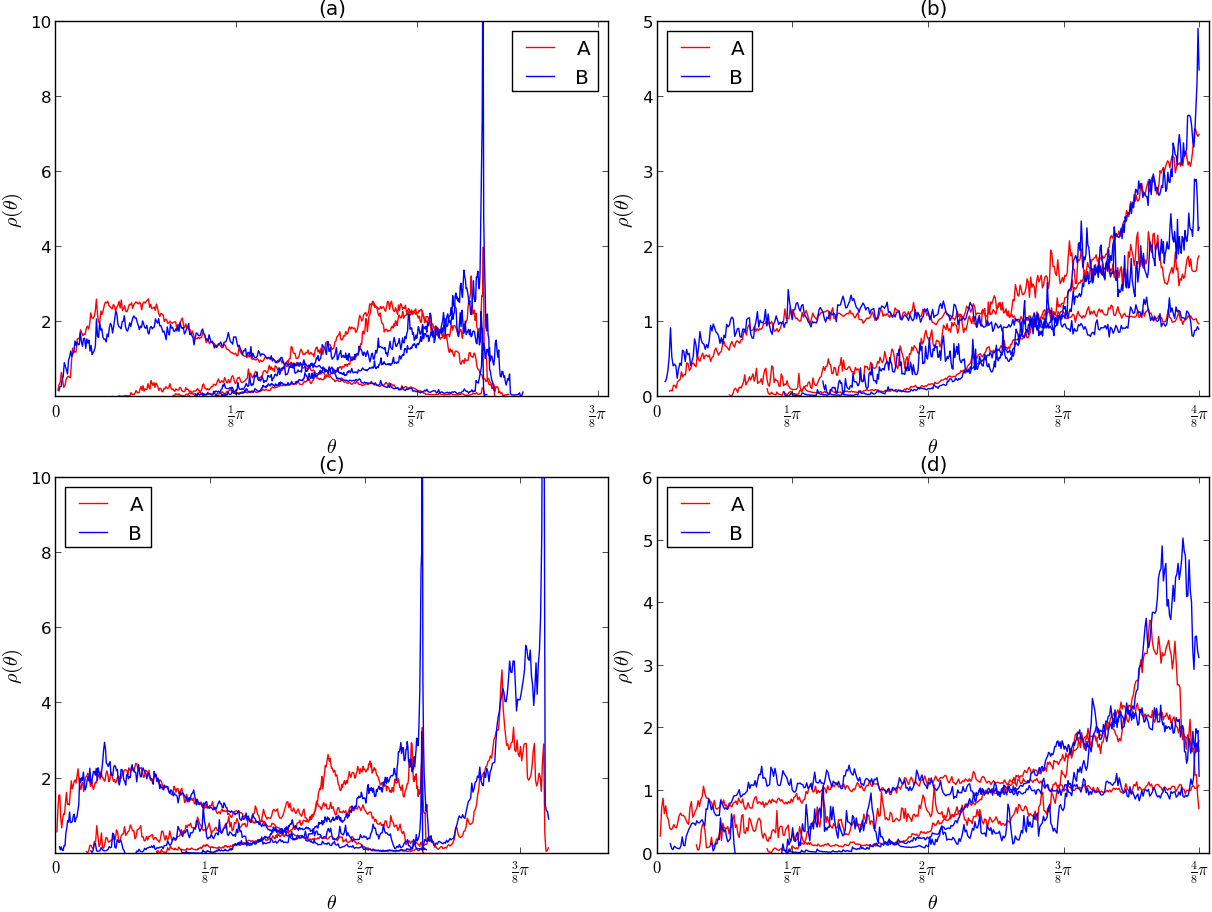
\includegraphics[width=1.0\textwidth]{statistic_angle_rpoppo_AB}
  \caption{Statistical result as in \reffig{fig:statistic_angle_rpoppo}
    with two types of orbits counted separately. Type A, B stand for the
    orbits with only one expanding directions and those with two expanding
    directions respectively. Each curve is normalized that the area under it
    is one.}
  \label{fig:statistic_angle_rpoppo_AB}
\end{figure}

\textbf{What is statistics of set of long orbits
(remove those shorter than - let's say 85)?}
Periodic orbits with $ 85 < T_p < 100$ are collected to give the
statistical result in \reffig{fig:statistic_angle_rpoppo_log_85}.
Again, there is no striking difference if only long orbits are taken
into consideration.
\begin{figure}[h]
  \centering
  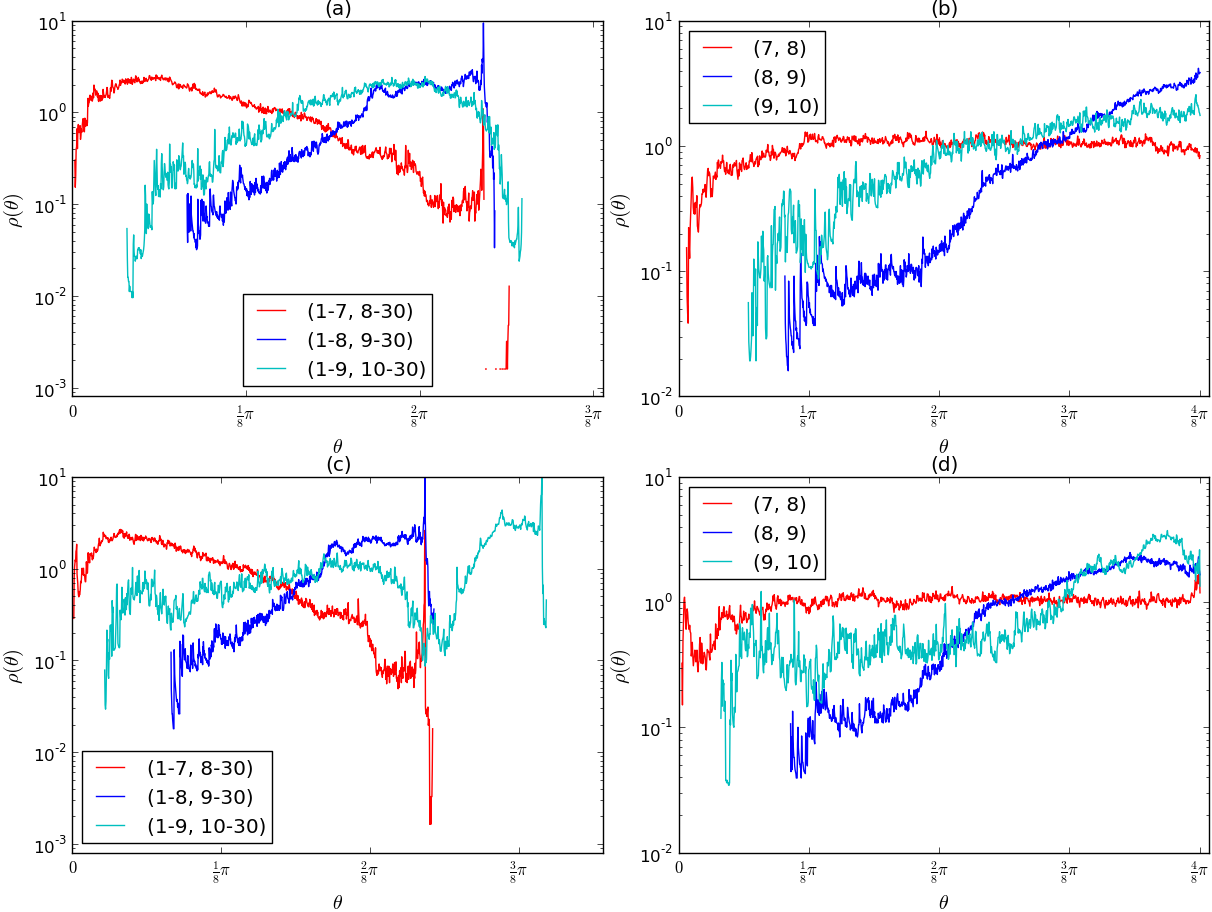
\includegraphics[width=1.0\textwidth]{statistic_angle_rpoppo_log_85}
  \caption{Similar to \reffig{fig:statistic_angle_rpoppo_log} but only count
  orbits whose period is larger than 85, that is, 131 out of 240 \cycle{ppo}s
  and 128 out of 239 \cycle{rpos}.
}
  \label{fig:statistic_angle_rpoppo_log_85}
\end{figure}

\textbf{why is the green curve so different between periodic orbits and relative periodic orbits?}
I am not sure, but I guess the reason lies on how we defined the subspace
spanned by the first 9 Floquet vectors. As I mentioned on the meeting,
if the 9th and 10th vectors form a complex conjugate pair, then both the
real part and the imaginary part will be counted to span the subspace.
For relative periodic orbits, the percentage of such orbits is 130/239, while
0\% for pre-periodic orbits; also, Floquet vectors with larger
index are more hyperbolicly disentangled from the physical mode. That is why
the angle between subspace (1-9) and (10-30) have a shift to large angle for
relative periodic orbits. On the contrary, for both \cycle{ppo} and \cycle{rpo},
the 8th Floquet vector never forms complex pair with the 9th one, so they
have similar distribution for angle between subspaces (1-8) and (9-30).

By the way, \cycle{rpo} is more prone to have complex conjugate Floquet vectors
than \cycle{ppo}. I think it is because the different definitions of Jacobian.
For \cycle{rpo}, $J_p = g_p J^{T_p}$. For \cycle{ppo}, $J_P = RJ^{T_p}$.
Here $g_p$ is a rotation, while $R$ denotes reflection.

\textbf{We do not know why there are sharp peaks at larger angles?}
From \reffig{fig:statistic_angle_rpoppo_AB}, we can see the peaks mainly
come from the orbits which have two expanding directions, but I still do not
know
why it should be like this. Also is this information very important?

\textbf{Maybe you could plot the intersection of the unstable manifold
of the orbit in \reffig{fig:ergodic_dis_angle_ppo4} with a {\PoincSec}
and the same for an ergodic orbit, and see if there is transverse
distance between them.} Pre-periodic orbit \cycle{ppo4} have two
expanding real directions with Floquet exponent 0.04 and 0.03
respectively. \refFig{fig:manifold_ppo4} gives its two dimensional
unstable manifold. following Chat\'{e}'s suggestion to look at the
local dimension at other points on this orbits, I found that I got
figure like \reffig{fig:ergodic_dis_angle_ppo4} on some points (black
dots in \reffig{fig:manifold_ppo4}); while some points on the orbit
(yellow dots in \reffig{fig:manifold_ppo4}) are capable to get the
local dimension. Does it mean that only part of \cycle{ppo4} is on the
attractor?

\refFig{fig:manifold_ppo4_m2} and \ref{fig:manifold_ppo4_m3} show how ergodic
trajectories intersect with {\PoincSec}. At least, we can identify two
different types of points I collected. I think that is why there are
two different structures
in \reffig{fig:ergodic_dis_angle_ppo4}. If \cycle{ppo4} has more than
one unstable bundle passing by the cluster, then we can say that the I am using
distance in a wrong way, but there is one unstable bundle penetrating the cluster,
so I still do not know why this template point fail to deduct information about
dimension. On the other hand, the 3d figures are just projections onto Fourier modes,
useful information may be lost.

\begin{figure}[h]
  \centering
  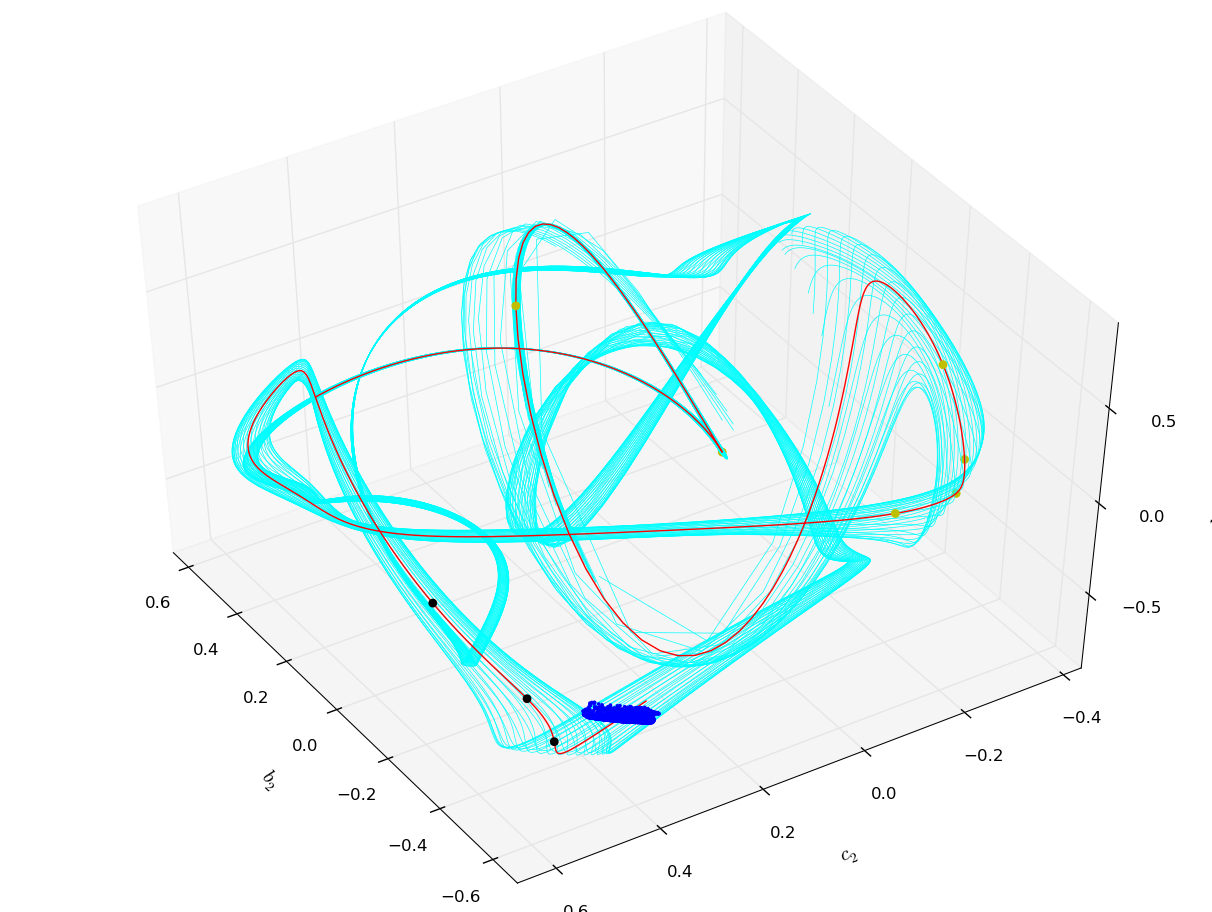
\includegraphics[width=1.0\textwidth]{manifold_ppo4}
  \caption{Unstatble manifold of \cycle{ppo4}. Red curve is the trajectory of
    \cycle{ppo4} for time $T_p = 33.38$. Black dots are the template points where I
    did not succeed to deduct information about local dimension; on the contrary,
    I did at yellow dots. The cluster of blue dots are the intersecting points between
    an ergodic trajectory and {\PoincSec} whose template point is the same as
    in \reffig{fig:ergodic_dis_angle_ppo4}. This figure is a projection onto the
    subspace of Fourier modes. x, y and z axes are $b_2$, $c_2$ and $b_3$ respectively.
  }
  \label{fig:manifold_ppo4}
\end{figure}

\begin{figure}[h]
  \centering
  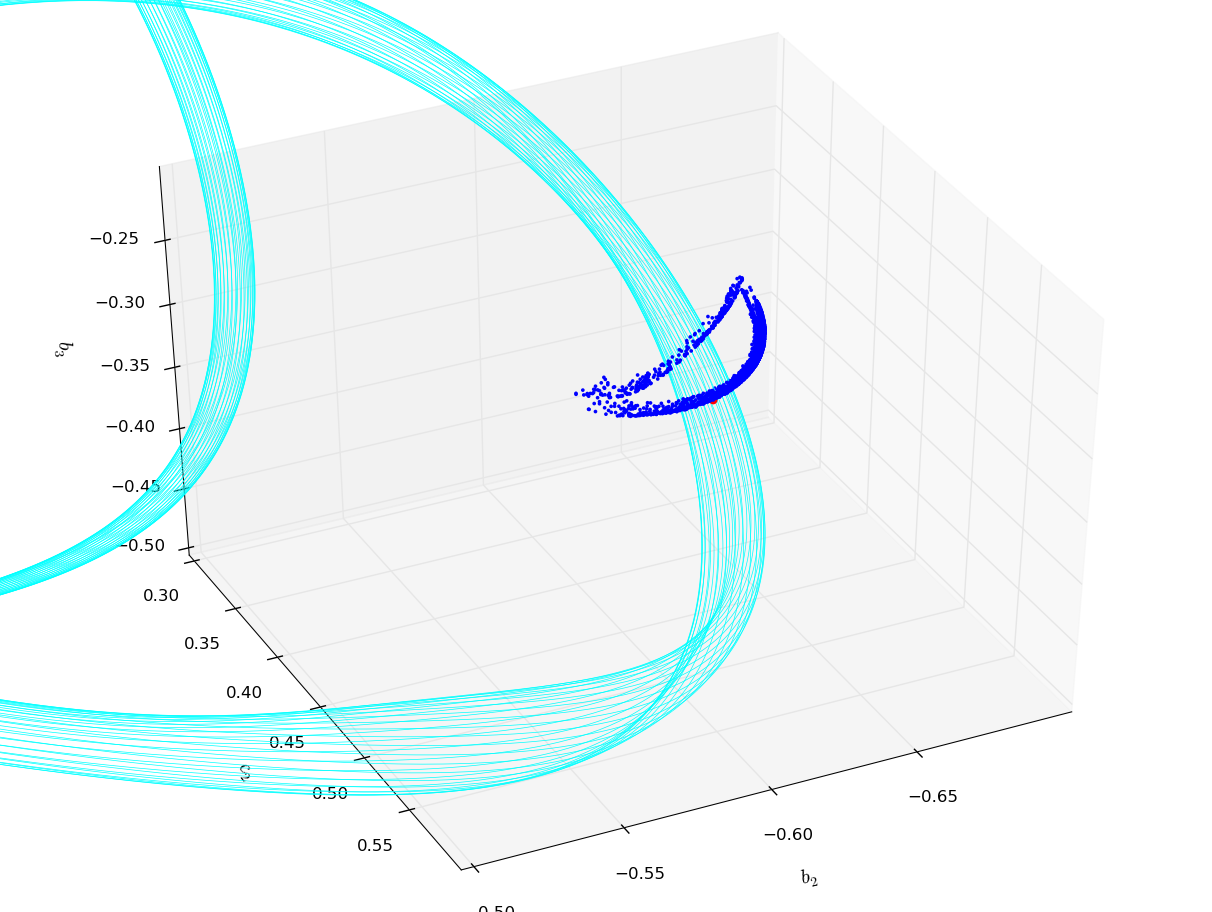
\includegraphics[width=1.0\textwidth]{manifold_ppo4_m2}
  \caption{The same as \reffig{fig:manifold_ppo4}. The part containing the cluster points
    are magnified. Red dot is the template point.
  }
  \label{fig:manifold_ppo4_m2}
\end{figure}

\begin{figure}[h]
  \centering
  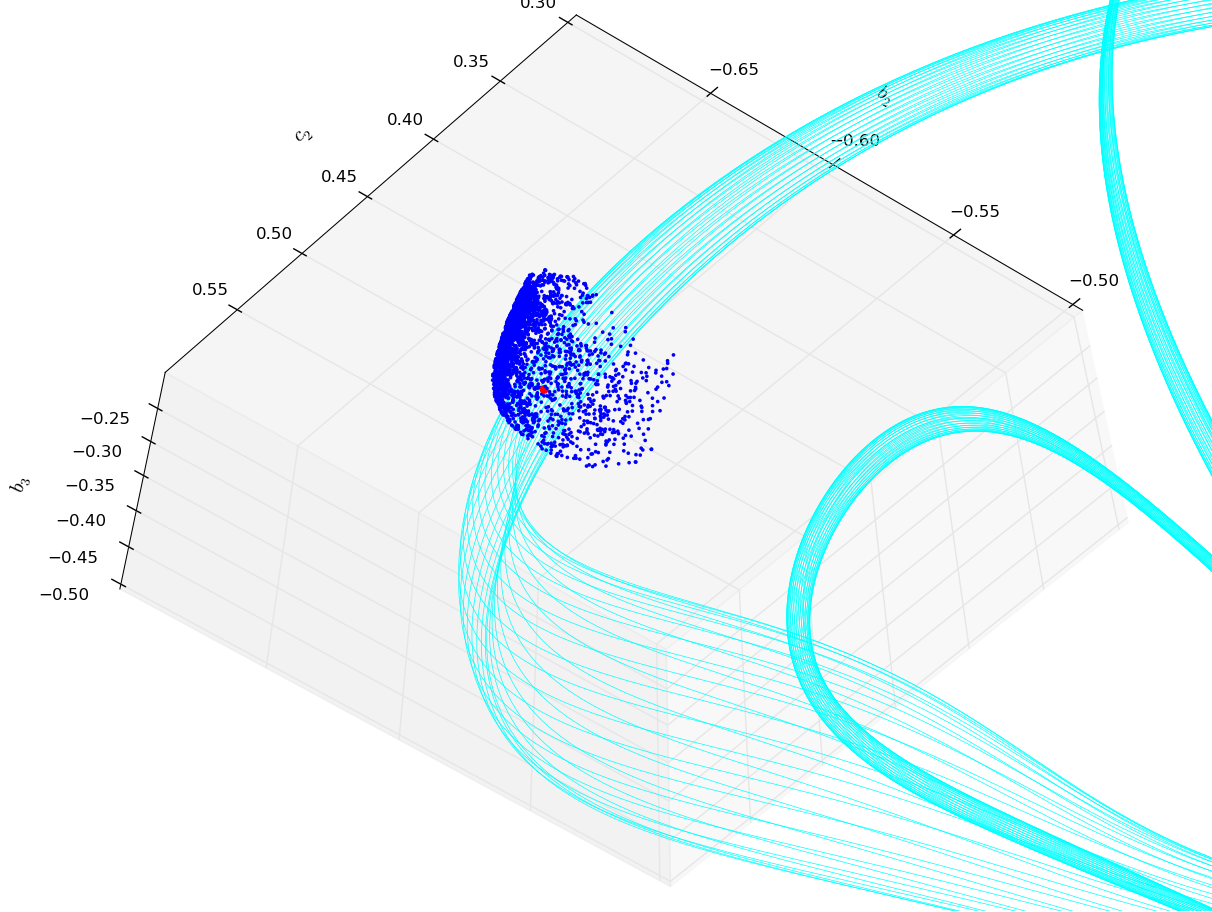
\includegraphics[width=1.0\textwidth]{manifold_ppo4_m3}
  \caption{The same with \reffig{fig:manifold_ppo4_m2} with a different angle.
  }
  \label{fig:manifold_ppo4_m3}
\end{figure}


\textbf{{\PoincSec} is a bit confusing in 3D. Could you plot a 2D projection?}
I am not sure whether 2d projection is better than 3d, and I tried 2d projection, It
does not seem more informative.

\item[2014-09-20 Evangelos] A brief summary of brainstorming session with Hugues and Xiong:

We think that \reffig{fig:ergodic_dis_angle_ppo4} is not as problematic as we initially thought.
The data points having small distance and large angle, presumably come from points that come close to
the ppo, but do not really shadow it. We suggested to Xiong to try to look only for points where the distance
is small and the ergodic trajectory stays close to the ppo for a while. Alternatively, he could test the
degree of alignment of the flow velocity at the close encounters. Basically apart from the condition
of distance being smaller than certain threshold, it might help to also impose the condition that the angle between
flow velocities is smaller than a threshold.

Regarding the data points with small distance and small angle for the red curve, we think that this is not
problematic. We understand this to mean that at certain points, tangent space can be spanned with fewer dimensions
than the 'attractor dimension.' We do not see a contradiction.

What worries us is that in some of the figures, e.g. \reffig{fig:ergodic_dis_angle_rpo1}, we see that as more
dimensions are taken into account the angle keeps getting smaller for what we think is the same point on the
trajectory. We believe that if the dimension of the attractor can be captured by the rpos, we should see an accumulation
towards a lower bound in angle. We suggest that Xiong adds more subspaces to these plots, to see if this happens.

If I understand this correctly, another way to state this, is that for a given point on the ergodic trajectory,
adding unphysical dimensions would lead to exponentially decreasing correction to the angle. Therefore it might help to
plot the correction in angle when you add an extra subspace, as a function of the number of included subspaces for a given point on a trajectory (a given difference vector).

Finally we think it might be worth looking at the variation of the smallest principal angle parametrized by time along a
rpo, for some rpos, both problematic and non-problematic.

\item[Xiong 2014-09-21] Some comments. \\
I updated \reffig{fig:ergodic_dis_angle_rpo1}. The original one is produced by
using the integrator in the 1st mode space; while all other figures are produced by
post-processing method. In order to keep the unitarity across all figures, I recollected
the intersection points for \cycle{rpo1} and found that \reffig{fig:ergodic_dis_angle_rpo1} only changes slightly. The original one is kept in the
svn repository.

\begin{figure}[h]
  \centering
  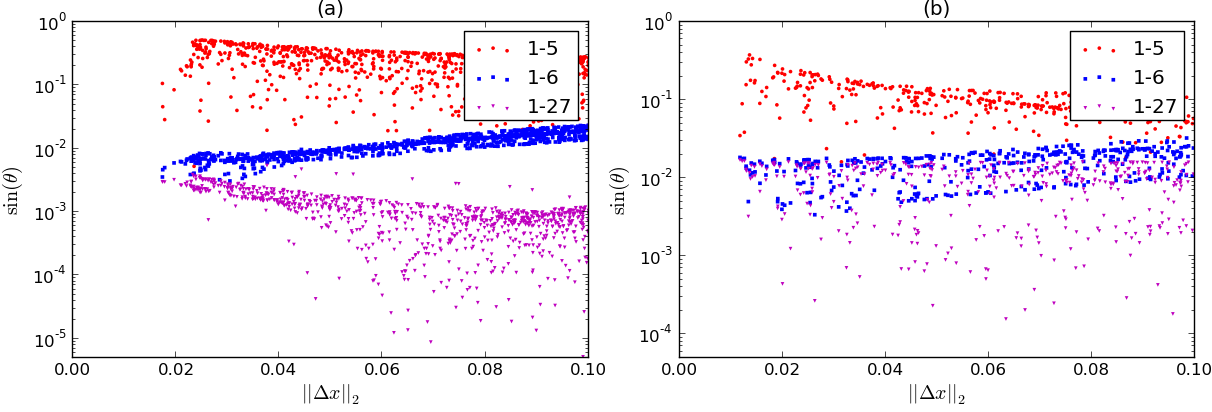
\includegraphics[width=1.0\textwidth]{ergodic_angle_rpo1_v2}
  \caption{The same as (b) (d) in \reffig{fig:ergodic_dis_angle_rpo1}
    except replacing $1-8$ by $1-27$.}
  \label{fig:ergodic_angle_rpo1_v2}
\end{figure}

\begin{figure}[h]
  \centering
  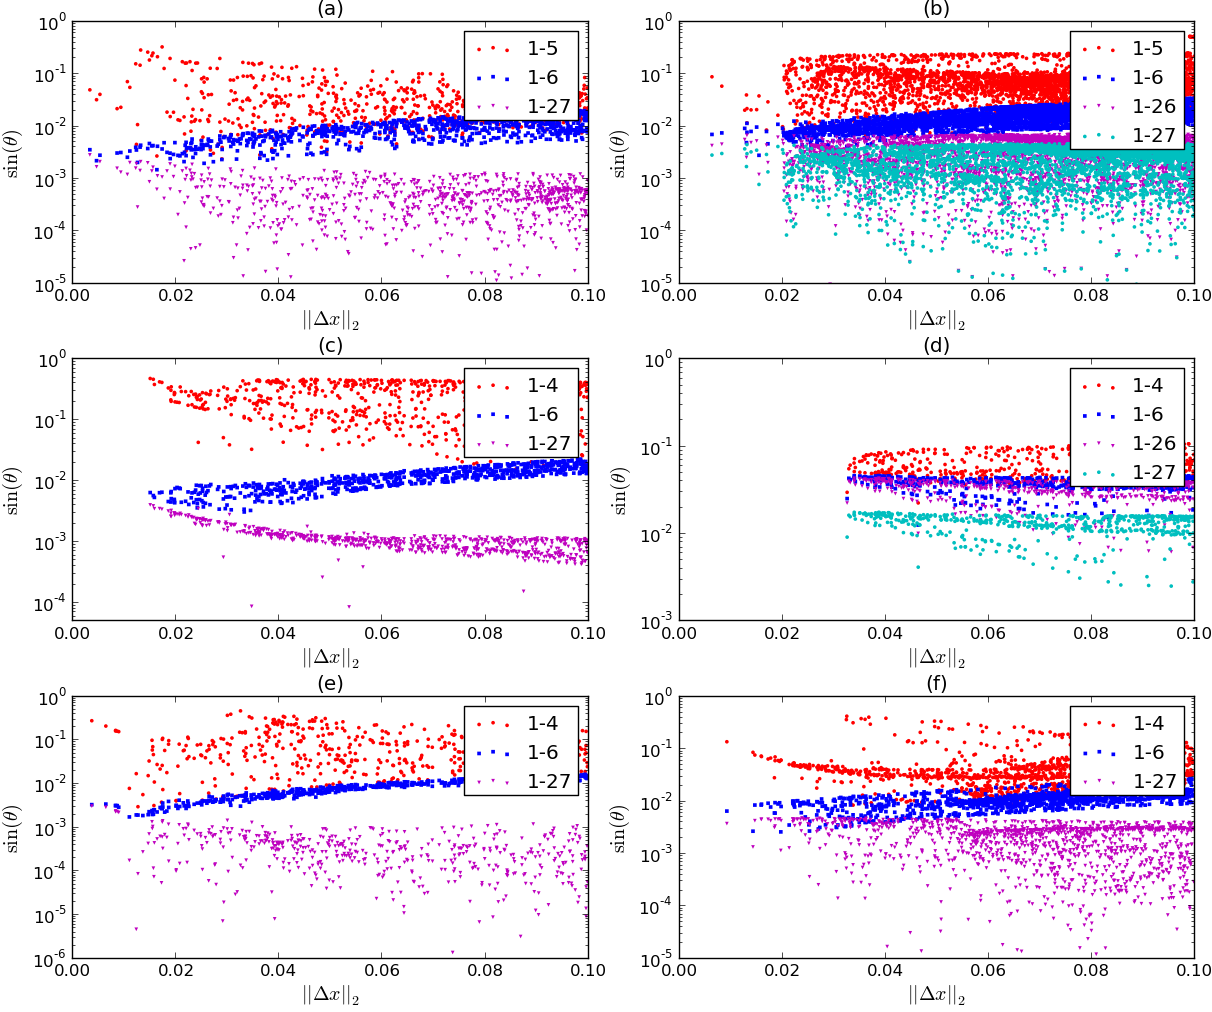
\includegraphics[width=1.0\textwidth]{ergodic_angle_collection}
  \caption{The same as \reffig{fig:ergodic_dis_angle2} except replacing case ($1-8$)
    by ($1-27$) or ($1-26$) .}
  \label{fig:ergodic_angle_collection}
\end{figure}

Dimensions are added to span the subspace when expanding the difference
vector. As shown in \reffig{fig:ergodic_angle_rpo1_v2}, angle tendency
for case ($1-27$) actually saturates with that for ($1-6$) when
difference vector decreases. The cases for other orbits are shown in
\reffig{fig:ergodic_angle_collection}. Note the dimension of this
system after slicing and {\PoincSec} is 28, so ($1-27$) refers to the
subspace spanned by all the Floquet vectors except the last one. As is
shown in these figures, the angle scattering points will indeed shift
down for large $||\Delta x||_2$ ($\gtrsim 0.04$), but they converges to
the case $(1-6)$ when these points get closer to the template point.
Looking at these figures makes me feel better about
\reffig{fig:ergodic_dis_angle_ppo4}. At the same time, we should be
aware of panel (b) (d) in \reffig{fig:ergodic_angle_collection}. It
seems that ($1-26$) saturate to ($1-6$) but not for ($1-27$) at these
two template points.

To investigate the velocity alignment between {\Poincare} intersecting points and
the template
points, \reffig{fig:velAngDistributionCollection} shows the angle distribution
for each template point in different orbits. Although \cycle{ppo4} has relatively large
portion in large angles $0.25$, it looks normal since \cycle{rpo3} also
behaves similarly. The other three cases have maximal angle around $0.16$. Also I tried
to exclude the intersecting points which are misaligned (velocity angle $\theta > 0.16$),
the result is similar to \reffig{fig:ergodic_dis_angle_ppo4}. Another way I tried to get rid
of the velocity misalignment is just recording even closer recurrence points. For all the
above experiments, the threshold of accepting a {\Poincare} intersecting point is that
the difference vector should have Euclidean length less than 0.1, but now I tried a
smaller threshold 0.02. The result is shown in \reffig{fig:ergodic_angle_ppo4_002}.
In this case, the velocities at {\Poincare} intersecting points are well aligned with
the velocity at the template points ($\theta < 0.07$). It is clear that 5 Floquet vectors
at this point are not enough to span the local space, and $(1-4)$, $(1-27)$ produce the
similar result.  But the figure is not sharp enough. It seems that smaller threshold is
required to see the tendency.

\begin{figure}[h]
  \centering
  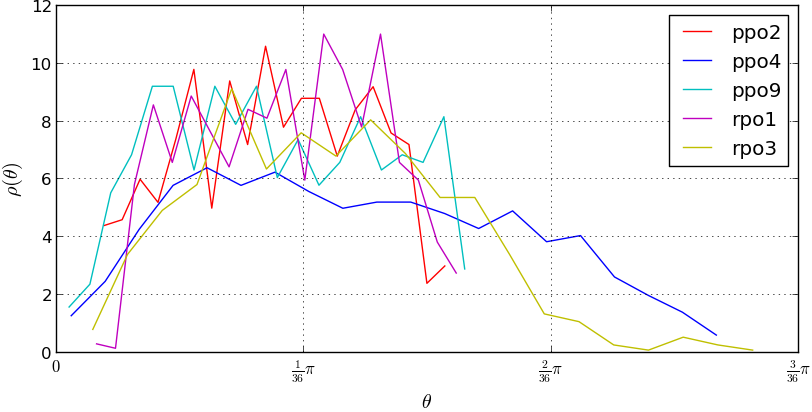
\includegraphics[width=1.0\textwidth]{velAngDistributionCollection}
  \caption{ Distribution of the angle between the velocities at the {\Poincare} intersecting
    points and the template point for different orbits. The template point is the farthest
    away from the slice border. 20 bins are used in this histogram plot and the area under
    each line is normalized. Sorry about the previous histogram plots, they are normalized
    incorrectly, and I will update them in future. But they will not change too much.
    }
  \label{fig:velAngDistributionCollection}
\end{figure}

\begin{figure}[h]
  \centering
  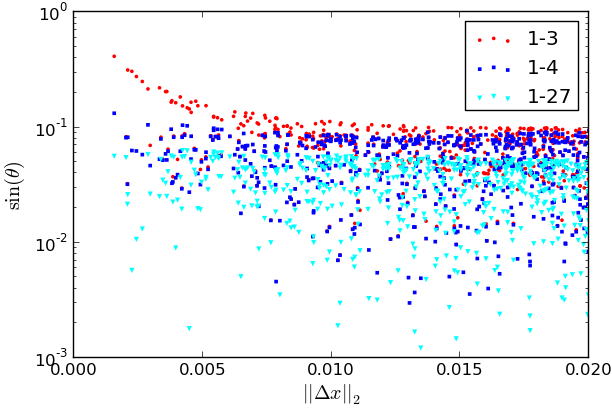
\includegraphics[width=0.7\textwidth]{ergodic_angle_ppo4_002}
  \caption{The same as \reffig{fig:ergodic_dis_angle_ppo4} but with closer
    intersecting points. 588 points were collected in a whole day. Note, here
    (1-3) (1-4) are used.
    }
  \label{fig:ergodic_angle_ppo4_002}
\end{figure}

\refFig{fig:hyperbolicitySample} shows how angle changes along the
three different orbits.

\begin{figure}[h]
  \centering
  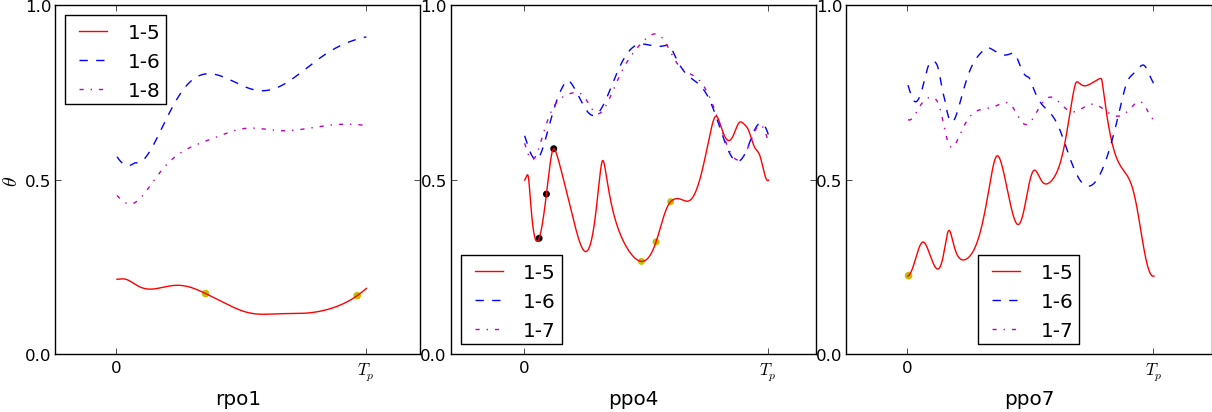
\includegraphics[width=1.0\textwidth]{hyperbolicitySample}
  \caption{The smallest principal angle between the subspace
    spanned by the Floquet vectors indicated by the legend and the one spanned
    by the remaining Floquet vectors. Three different orbits are used here.
    Yellow dots donate the non-problematic points;  black dots donate the
    problematic points.
    }
  \label{fig:hyperbolicitySample}
\end{figure}

\item[2014-09-23 Kazz to Xiong and everyone]
I enjoyed the updates. Here are my comments, suggestions, and questions.
A skeleton of the paper follows.

\textbf{Distribution of principal angles.}
The results in \reffig{fig:statistic_angle_rpoppo_log}
(log-scale plot of \reffig{fig:statistic_angle_rpoppo}) are nice,
 but not enough to claim that the blue and turquoise distributions are bounded
 away from zero.
It's true you don't have data for $\theta$ close to zero,
 but if you extrapolate, I would say the distributions decrease exponentially
 with $\theta$ (look straight in \reffig{fig:statistic_angle_rpoppo_log})
 and reach non-zero densities at $\theta = 0$,
 so the physical and unphysical subspaces are not strictly split.
To claim that these distributions are bounded, data must be fitted with
 a function that is bounded or has an essential singularity at $\theta =0$
 (e.g., $\rho(\theta) \sim \exp(-\text{const.}/\theta)$).
You say ``Distribution $\rho(1/\theta)$ is not used here
to show the boundedness because I did not get a good exponential relation'',
 but how bad was it?
How difficult is it to accumulate more statistics
 so that the tail of the pdfs extends by, say, one more digit?
As these will be the central results of the paper,
 I am most concerned with this problem.

\textbf{Angle vs distance plots.}
As I mentioned in the web discussion,
 if a given subspace covers the physical subspace,
 one would expect a linear relationship between the angle and the distance,
 as shown in \refref{TaCh11}.
This is because, in this case,
 the only reason the difference vector is not in the subspace
 is that the physical manifold deviates from its linear approximation
 as the distance increases.
If we assume that the manifold is smooth
 (as should be if it corresponds to the inertial manifold),
 the deviation from the linear approximation is
 in the order of $||\Delta r||_2^2$ in distance,
 so, in angle, $||\Delta r||_2^2 / ||\Delta r||_2 = ||\Delta r||_2$.
Therefore, I suggest to plot \reffig{fig:ergodic_dis_angle_rpo1}
 and similar figures in loglog scales, and compare the slope with -1.

\textbf{Concerning \reffig{fig:ergodic_dis_angle_ppo4}.}
I agree with what is written in the brief survey of the brainstorming session.
It is particularly important to understand why the blue and purple dots
 do not approach zero as the distance decreases.
It would be perfect if this is caused by ergodic trajectories that come nearby
 but not shadow the orbit (I found this very interesting), but the result
 in \reffig{fig:velAngDistributionCollection} doesn't seem to be convincing.
I have an alternative suggestion:
 you can decompose the difference vector
 using the bases given by the Floquet vectors,
 and see how each component grows/shrinks with time.
If the trajectory is topologically close to the orbit,
 each component should grow or shrink at the corresponding Floquet exponent.
One may use it as a criterion
 to distinguish topologically close orbits and others.
Of course, to check this idea,
 one should compare problematic and non-problematic orbits along this line
 and see if the above speculation is correct.

\textbf{rpo vs ppo?}
It seems that the ensemble of rpos and that of ppos
 produce essentially the same result (\reffig{fig:statistic_angle_rpoppo_log}),
 which is very nice.
But then, what do you think is the role of rpos?


\textbf{Provisional structure of the paper.}
Assuming that all above pending problems will be resolved,
 here is what I propose for the structure of the paper.

\begin{enumerate}

\item Introduction
\begin{itemize}
\item Introduce the periodic orbit expansion of chaos.
Describe how powerful it is (e.g., to compute dynamical averages),
 and more importantly, how conceptually important it is
 (orbits form the skeleton of chaos).
Stress however that it is unclear to what extent this picture is valid
 for spatially extended systems
 (briefly mention what is known and what is missing).
\item Explain main results in \refref{YaTaGiChRa08,TaGiCh11}
 (decoupling of the physical/spurious subspaces).
This approach seems to be well suited for the periodic orbit description,
 because all the necessary quantities (Lyapunov exponents/vectors)
 can be defined for the orbits as well,
 in terms of the Floquet exponents and vectors.
However, applying the same method to an orbit makes no sense,
 because the length of an orbit is finite,
 so the angle distribution of any pair of vectors is bounded.
One should look at an ensemble of orbits!
\end{itemize}

\item Methods
\begin{itemize}
\item system, numerical integration, algorithm to find orbits,
 algorithm to compute Floquet exponents/vectors and their precision
 (precision is important because usually it's difficult to obtain
 strongly contracting Floquet modes).
\end{itemize}

\item Main results
\begin{itemize}

\item Figure 1: Visualize how an ergodic trajectory approaches an orbit.
Figure like \reffig{fig:xdpo1ppo191} between an ergodic trajectory and an orbit
 is good enough. Showing how the Euclidean distance evolves is even better
 (like Fig.2b in \refref{TaCh11}).

\item Figure 2: Display a figure like \reffig{fig:statistic_angle_rpoppo_log}.
We need a clear figure (so clear data and/or analysis) to show that
the distribution becomes bounded as soon as the subspace includes
 a certain number of Floquet vectors.
Compare this number with the physical dimension
 estimated from the ergodic trajectories
 (which is nine, including three neutral modes; see Fig.4a in \refref{TaCh11}).

\item Figure 3: Display a figure like \reffig{fig:ergodic_dis_angle_rpo1}
 or \reffig{fig:ergodic_dis_angle2}, which shows that each orbit carries
 information of the physical dimension
 (we however need to use ergodic trajectories here;
 to construct the physical dimension purely from orbits,
 one needs an ensemble).
However, we first need to understand \reffig{fig:ergodic_dis_angle_ppo4}.

\item It would be wonderful
 if we find an orbit indicating a smaller physical dimension
 (as the brainstorming session discussed
 about \reffig{fig:ergodic_dis_angle_ppo4}, but without strange behavior
 of the blue/purple dots).
Try to find such an orbit, and if you do so, look for anything particular
 about this orbit (in particular, hyperbolicity).
If we succeed in doing this, we can discuss relation
 to the dimension variability (see, e.g., \refref{KaGrPrLaSi02}).
This will significantly increase the impact of the paper,
 because this is something that we cannot do solely with ergodic trajectories
 (at least at present).
\end{itemize}

\item Conclusion.
\end{enumerate}

Any comments and suggestions are welcome, of course!
\begin{figure}[h]
  \centering
  \includegraphics[width=1.0\textwidth]{ergodic_angle_ppo1}
  \caption{The same experiment as in
  \reffig{fig:ergodic_angle_ppo4_002} conducted on \cycle{ppo1}. The
  blue, red and green points refers to subspace (1-5), (1-6)
  and (1-27) respectively. 2864 points are recorded.
}
  \label{fig:ergodic_angle_ppo1}
\end{figure}

\item[Xiong 2014-10-10]
  I am not sure what I understand about angle distributions is
  correct or not.

  \textbf{dominated splitting} was invented as a relaxed version of
  hyperbolicity since the latter is a very strong property or restriction.
  According to\rf{Enrique03}, an f-invariant set
  $\Lambda$ is said to have dominated splitting if the tangent bundle can
  be decomposed into two continuous invariant subbundles
  $T_\Lambda M = E \oplus F$, such that:
  \[
  ||Df^{n}_{/E(x)}||\cdot||Df^{-n}_{/F(f^n(x))}|| \le C\lambda^n \,,\quad
  \text{for all} \quad x\in\Lambda\,, n\ge 0
  \]
  with $C>0$ and $0<\lambda<1$. In my view, it is
  $||J^n(u)||/||J^n(v)||\le C\lambda^n$ for $u\in E$ and $v\in F$.
  Basically, it means that the expanding rate in subspace $F$ is larger
  than the expanding rate in the subspace $E$ at every instant point along
  the trajectory. This definition leads to the boundedness of angle
  between these two subspaces $\angle (E, F)$. Let $\lambda'=C\lambda$, then
  \[
  ||Ju|| \le \lambda' ||Jv|| = \lambda'(||J(v-u)||+||Ju||)
  \]
  so
  \[
  ||v-u|| \ge \frac{1-\lambda}{\lambda}\frac{||Ju||}{||J||}
  \]
  Here, you can regard the matrix norm as the vector induced Euclidean
  norm $||A||=\max(||Ax||_2/||x||_2)$, therefore the angle between these
  two subspaces is bounded away from zero.

  Jairo points out (proposition 3.1 in\rf{Bochi05} or proposition 2.3
  in\rf{Bochi04}) that if the dominated splitting is not satisfied at
  point $y$, then there exists an $(\epsilon_0,\kappa)$-realizable sequence
  ${L_0, \cdots, L_{m-1}}$ at y such that
  \[
  L_{m-1}\cdots\L_0(v) = \omega
  \,,
  \]
  where $v\in E$ and $\omega\in J^{m}(F)$. I am sorry I could not fully
  understand this proposition, but it seems that if the dominated
  spitting is not satisfied, then there is possibility that vectors in
  one subspace can evolve into another subspace at sometime, which means
  these two subspaces may get entangled at some point along the trajectory.

  What confused me is the physical picture of tangency (angle be zero).
  If tangency happens, it means that the set of covariant vectors are not
  linearly independent, so they does not span the whole tangent space.
  The only possibility I could get up with is that Jacobian matrix $J_p$
  does not have a whole set of Floquet vectors. Just like matrix
  $\bigl(\begin{smallmatrix}
    1&1\\ 0&1
  \end{smallmatrix} \bigr)$
  has only one eigenvector:
  $\bigl(\begin{smallmatrix}
    1\\ 0
  \end{smallmatrix} \bigr)$.
  The periodic eigendecomposition will give you two same eigenvectors then.
  However, numerically, these two eigenvectors can not be exactly same.
  What do you think ?

  Pavel V.Kuptsov uses principle angles to investigate the hyperbolicity
  of a chaotic system. In \refref{Kuptsov12}, Fig.1 is very similar to our
  result \reffig{fig:statistic_angle_rpoppo_log}. Since \KS\ system is not
  hyperbolic, we are actually testing dominated splitting, but the idea is the
  same. Also if we QR and LQ decompose the eigenvector matrix $v=Q_1R=LQ_2$ and
  define $P=Q_1^\top Q_2$, then, as Pavel points out,
  submatrix $P(1:k,1:k)$ is singular, which is in accordance with my picture.

  I think I will try to investigate the dominated splitting of these \cycle{rpo}
  and \cycle{ppo}.
%Also I am still working on the problems left from last meeting. but the
%progress is very slow. I am sorry about it.

  \begin{table}[h]
    \centering
    \begin{tabular}{c  c | c c}
      E & $\rho$ & E & $\rho$  \\ \hline
      1-1  &     0.487   &   1-9  &           0 \\
      1-2  &     0.336   &   1-10  &          0 \\
      1-3  &     0.178   &   1-11  &          0 \\
      1-4  &     0.059   &   1-12  &          0 \\
      1-5  &     0.029   &   $\cdots$ & 0       \\
      1-6  &     0.017   &   1-28  &          0 \\
      1-7  &     0.008   &   1-29  &          0 \\
      1-8  &     0       &         &            \\
       \\
       \\
       \\
       \\
         \\
       \\
       \\
    \end{tabular}
    \caption{Percentage of violence of dominated splitting for
      \cycle{rpo} and \cycle{ppo} whose period is less than 100.
      The zeros in the table are exact. $E$ is the subspace spanned
      by the indexed Floquet vectors.
    }
    \label{tab:dominated_splitting}
  \end{table}

\item[2014-11-26 Xiong Ding]

I conducted a series of new experiments in order to resolve the
problems proposed by the last meeting. First, I use part of periodic
orbits with $ 100 < T < 120$ to collect the angle distribution as
previous did in \reffig{fig:statistic_angle_rpoppo}. I find that the
distribution is rather stable. Second, I give up {\PoincSec} and turn
to use human labor to inspect each approaching incidence in
\reffig{fig:ergodic_angle_rpo1_v2} to locate the true shadowing part
approximately. In this way, I obtained a better angle-distance
scattering plot \reffig{fig:disAngScatter_ppo4}.
\begin{figure}[h]
  \centering
  \includegraphics[width=0.48\textwidth]{angle120ppoSpace1} \hfill
  \includegraphics[width=0.48\textwidth]{angle120ppoSpace2}
  \caption{Angle distribution $\rho(\theta)$ versus $\theta$
    for \cycle{ppo} which has $ T < 120$.
    Left: angle distribution for subspace indexed up to 22.
    Right: angle distribution for subspace from 23 to 29.
  }
  \label{fig:angDist_ppo}
\end{figure}
\begin{figure}[h]
  \centering
  \includegraphics[width=0.48\textwidth]{angle120rpoSpace1} \hfill
  \includegraphics[width=0.48\textwidth]{angle120rpoSpace2}
  \caption{The same as \reffig{fig:angDist_ppo}, but for \cycle{rpo}s.
  Note that subspace cut at 11, 13, 15, 17, 19, 21 are not plotted
  because the sample points are very few. For example, the 16th, 17th
  Floquet vectors form a complex pair
  for all \cycle{rpo}s, so the collected
  data for (1-16,17-30) is zero.}
  \label{fig:angDist_rpo}
\end{figure}
\begin{figure}[h]
  \centering
  \includegraphics[width=0.48\textwidth]{angle120ppoVector1} \hfill
  \includegraphics[width=0.48\textwidth]{angle120ppoVector2}
  \caption{ Angle distribution for Floquet vectors with adjacent
    indices for \cycle{ppo}.
  }
  \label{fig:angDistVec_ppo}
\end{figure}
\begin{figure}[h]
  \centering
  \includegraphics[width=0.48\textwidth]{angle120rpoVector1} \hfill
  \includegraphics[width=0.48\textwidth]{angle120rpoVector2}
  \caption{The same as \reffig{fig:angDistVec_ppo} but for \cycle{rpo}.
  Note a lot of cases are omitted because either Floquet vector is
  complex.
}
  \label{fig:angDistVec_rpo}
\end{figure}

In \reffig{fig:angDist_ppo}
, angles between subspaces spanned by
Floquet vectors are collected for \cycle{ppo}, \cycle{rpo} with
period $ 100 < T < 120$, in contrast to the previous experiments
with $T < 100$.
\Xiong
{2014-11-27}
{Not all of the orbits with $100 < T < 120$ are used. For some
of them, my multishooting routine fails to refined them because some
of the long orbits converge to short orbits. Only 85 percent of them
are used to do the statistical experiments. Even though, the number
of orbits considered here is much more than the orbits with $T < 100$.}
Several points need to be mentioned.
First, we observe that the angle distribution is
rather stable. Data collected from $T < 100$ with that
collected with $100 < T < 120$ has similar shape. For instance,
\reffig{fig:angDist_ppo} is very close to
\reffig{fig:statistic_angle_rpoppo_log_85}. This means that this
distribution is a result of the geometrical structure of the
inertial manifold of this system (although the relation is unknown
until we find the symbolic dynamics).
It demonstrates that  short periodic orbits consist
of the skeleton of an ergodic system, and, in future,
studying only the fundamental POs is enough  to get the physical dimension of
a system. Second, \cycle{ppo}s and \cycle{rpo}s are still treated
separately because I find that the angle distribution for 8th and 9th Floquet
vectors is zero for \cycle{ppo} but not for \cycle{rpo}
\reffig{fig:angDistVec_ppo} and \reffig{fig:angDistVec_rpo}.
I guess the difference is related to the different definition of Jacobian
for \cycle{ppo} and \cycle{rpo}. For rpo, a rotation matrix is multiplied
to Jacobian, and it mix the real and complex component of Fourier modes.
So in \reffig{fig:angDist_rpo}, angle distribution of (1-10) vs (11-30) is
plotted other than (1-9) vs (11-30). On the other hand, no matter whether
there is tangency between 9 and 10, these two directions are both
contracting, their tangency would not change the local dimension.

\begin{figure}[h]
  \centering
  \includegraphics[width=0.8\textwidth]{disAngScatter_ppo4}
  \caption{Angle distribution versus length of difference vector for
    \cycle{ppo4}. Each point
    is an experimental incidence. Since we are on the slice, (1-6) corresponds
    (1-7) in the full state space. There are total 22592 shadowing points in
    this graph coming from collecting 700 ``V'' shapes.
  }
  \label{fig:disAngScatter_ppo4}
\end{figure}

\begin{figure}[h]
  \centering
  \includegraphics[width=0.48\textwidth]{disStructure_ppo4}
  \includegraphics[width=0.48\textwidth]{disStructure_ppo4_2}
  \caption{Two shadowing examples. Y axis is Euclidean length of
    difference vector. X axis is time.}
  \label{fig:disStructure}
\end{figure}

\begin{figure}[h]
  \centering
  \includegraphics[width=0.8\textwidth]{disAngAverage_ppo4}
  \caption{Averaged version of \reffig{fig:disAngScatter_ppo4}.}
  \label{fig:disAngAverage_ppo4}
\end{figure}

Also, I gave up the idea of {\PoincSec} when testing the relation
between angle distribution and length of difference vector. So only
slice is used to reduce the dimension by one, and Floquet vectors are
projected to the slice. Previously, we have a lot of substructures in
the $\sin(\theta)$ versus $||\Delta x||_2$ plot, but now, as shown in
\reffig{fig:disAngScatter_ppo4}, the substructures are gone. Also, the
concern that the angle-distance plot may  saturate for small difference
vector is not a problem, because data for distance as small as
$10^{-2.6}$ does not show any flatting tendency.

Figure \ref{fig:disAngScatter_ppo4} also shows that \cycle{ppo4}
is not problem any more, as contrast to used to be.
The problem is that when collecting data, we should make sure
that the ergodic orbit is indeed shadowing the PO, not just passing around.
This is difficult in numerical simulation since the unstable manifold of POs
are folding around the orbit.
Small Euclidean distance does not suffice to indicate
shadowing because small Euclidean ball around
one point along the Po may contain several
layers of unstable manifold. To resolve this problem, I take the procedure
as follows. First, we define a threshold trapping time $\tau_0$
and only collect approaching incidences which are trapped by the Po
for at least $\tau_0$. This will
substantially reduce the fake shadowing incidences. Second, although, the
ergodic segment found in the first step is trapped for a long time, it does
not mean that the whole segment is really shadowing the Po. It is highly
possible that only a part of the segment is, but the other part has crossed
the  unstable manifold and land on another layer of it.  So, in this step, we
need to observe the distance - time plot \reffig{fig:disStructure}
to find the real shadowing part. This is done by a graduate student's nude
eyes.

The V shape in \reffig{fig:disStructure} enclosed by two arrows
is the true shadowing incidence. An ergodic trajectories is attracted
by Po in the first part, and is pushed away by the Po in the second part.
There is a slight oscillation in the middle
valley because the ergodic point switches between stable manifold and unstable
manifold there. At the same time, it is hard for an ergodic orbit
to follow the stable manifold for a long time, as opposed to following
unstable manifold. As a consequence, there is a large percentage
of broken ``V'' shape (\reffig{fig:disStructure}(b)) in approaching incidence
profile, and in this case, we only record the points on the right segment.
Those V shapes with no oscillating valley are not recorded because I doubt
they are not switching between stable/unstable manifolds, but at the ridge
of a stable/unstable manifold witch has a shape curvature.

When choosing threshold trapping time $\tau_0$, smaller one will give us
more shadowing incidences; while, larger one will result in closer
approach. I tried a few different $\tau_0$s, I can only get approach as close
as $10^{-3}$.

Figure \ref{fig:disAngAverage_ppo4} gives the averaged angle distributions.
For (1-i) with $i < 7$, the angle density blows up or gets flattened as
$||\Delta x||$ decreases. (1-7) is almost a straight line with slope 1, but
the left most part has a small fluctuation. for (1-i) with $i>7$, they first
decrease as distance decreases, but at some point, they all saturate to
(1-7). This is reasonable, because when distance is large, omitting the last
few Floquet vectors does not have a large influence on angle. Note that, the
power spectrum of difference vectors almost concentrate on the first few
modes; while, when distance is large, the first 7 Floquet vectors are good
enough to expand the difference vector, so they saturate to (1-7).

\item[2014-12-08 Evangelos] I just had a look at the data for RPO$_4$. Period is
$T=33.4$, there two unstable directions with multipliers $\Lambda_1=4.4$, $\Lambda_2=-3.5$
and all other multipliers are real (I hope Xiong could verify this). Now I am a bit
confused as to where the oscillations in \reffig{fig:disStructure} come from,
since there are no complex multiplier pairs.

\item[2014-12-10 Hugues] In \reffig{fig:angDist_ppo} and \reffig{fig:angDist_rpo}:
these figures should be redone with all orbits (both "short" and "long").
importantly for each orbit, one should pay attention to "degeneracies" intheir
Floquet spectrum. I.e.: if the dimension of the manifold we want to consider falls
"in between" a degenerate subspace formed by a pair of Floquet eigenvalues, then
this orbit should not be included for that dimension. Also, we would like to see
this figure with more subspace dimensions than those currently shown, in particular
larger dimensions than the largest shown, in order to see whether the distribution
of angles goes away from zero as the dimension is increased. Also info about smaller
dimensions than the smallest shown could be intersting. All this for our internal
use, not necessarily to include in a paper.

\item[2014-12-10 Hugues] In \reffig{fig:disAngScatter_ppo4}:
How does it split if one considers only the down-going part of the Vs (and the
up-going parts)? What deos it look like if one only uses the local minima of the
time series of the distance, irrespective of that distance. This has the advantage
of exploring much smaller distances than those probed by the manual selection
method, and, very importantly, it does not require any manual intervention.

If plotting local minima gives some "satisfactory" answer, then similar figures
should be built using other orbits, including the short ppo1 orbit used by Kazz
before.

Then again, how would such a figure look like for an orbit which is "almost
non-hyperbolic", i.e. those orbits participating to the small-angle tail in fig.42?
could we see that the magic dimension is changed?


\item[2014-12-10 Hugues]
How about generating upo for a case with fixed boundary conditions, large enough to
be of significantly different dimension than the one treated so far? and then re-do
the whole thing... this is just to annoy Predrag...!


\item[2014-12-10 Xiong to Evangelos, Hugues]
I use \cycle{ppo4} because the previous results about this
orbit is terrible \ref{fig:ergodic_dis_angle_ppo4}. The
largest two Floquet multipliers are indeed 4.4 and -3.5,
but I find that the slops of `V' shapes vary and do not
follow these two numbers. I assume that this is because
we are measuring Euclidean norm not the distance along the
(un)stable manifold. For the oscillation, initially, I
just attribute it to the switching process between stable and unstable
manifolds, and presume that this process is accomplished
not immediately but in a few steps, so oscillation happens.
Now it is clear  that this explanation is not satisfactory,
I will look closer at this approaching incidence. By the way,
\cycle{ppo1} and \cycle{rpo1} also have such oscillation when
distance gets smaller than $10^{-2}$.

I will rerun my code to generate data following Hugues' advice.
It may take two or three days (I am preparing for a final exam these
two days:)). Thanks very much for writing down these requirements.
But when dealing with different boundary conditions,
this task may take more than a few days.
I do not know whether there is existing repository
documenting these \po s for this new setting.
In my side, it almost requires me to rewrite
the code of integrator and try to find a few hundred \po s
before conducting any experiments.

I will work tomorrow. Thanks.

\item[2014-12-12 Evangelos to Xiong] There are two things that I could think
these oscillations might tell us: 1) We are not in the linear
neighborhood of the PO (otherwise everything would be controlled by
{\stabmat} eigenvalues), 2) Below some distance between orbits, you reach
the limits of spatial resolution, so you cannot really distinguish
between the PO and neighborhing orbits.

I can see from Ruslan's database that this particular orbit was very
frequently detected, so I would guess that it must leave in the attractor
and we should be able to reach its linear neighborhood. Option (2) is more
likely since we know that refining the orbits by doubling the number of
modes changes the period to third significant digit. So you might want to
try the same computation with twice as many modes.

\item[2014-12-12 Xiong to Envangelos]
  If the modes are doubled, the initial condition has changed by 3 digits,
  but does it means that they are just slightly
  different points in the same orbit but not that more modes increase
  resolution dramatically?

\item[2014-12-12 Xiong]
  Figure \ref{fig:angDist_ppo} \ref{fig:angDistVec_ppo},
  \ref{fig:angDistVec_rpo} and \ref{fig:angDist_rpo} are updated with
  more subspace cases. Also $T<100$ and $100<T<120$ are combined.
  At right panels, angle extended to zero for subspace cut at
  odd indices. I guess it is because the time step I am using (h=0.02) is
  too large to separate the two modes which correspond to two nearly
  degenerate Floquet exponents for large indices.
  I remember once Kaza told me he used much
  smaller time step in his simulation. Anyway, the left panels are
  pretty convincing. Need I decrease the time step and
  redo all computation? That means a lot of coding.

\item[2014-12-15 Xiong]
  \refFig{fig:disAngScatter_ppo4} is updated in
  \refFig{fig:disAngScatter_localMin} with only points with minimal
  distance. The distribution diverges as distance decreases.
  \begin{figure}[h]
    \centering
    \includegraphics[width=0.48\textwidth]{disAngScatter_ppo4_localMin}\hfill
    \includegraphics[width=0.48\textwidth]{disAngScatter_rpo1_localMin}
    \caption{Left: for \cycle{ppo4}.
      The same with \reffig{fig:disAngScatter_ppo4} but only
      the local minimal point in each shadowing incidence is recorded. Right:
      for \cycle{rpo1}.}
    \label{fig:disAngScatter_localMin}
  \end{figure}


\item[2014-2-11 Xiong]
I tried to double the number of Fourier modes to integrate the system and
for Floquet vectors calculation.The new plots are generated in
\reffig{fig:disAngScatterN32_1} and \reffig{fig:disAngScatterN32_2}.

 \begin{figure}[h]
    \centering
    (a)\includegraphics[width=0.45\textwidth]{disAngScatter_ppo1x10}\hfill
    (b)\includegraphics[width=0.45\textwidth]{disAngScatter_ppo2x10sT30}
    (c)\includegraphics[width=0.45\textwidth]{disAngScatter_ppo3x10sT30}
    (d)\includegraphics[width=0.45\textwidth]{disAngScatter_ppo4x10}
    (e)\includegraphics[width=0.45\textwidth]{disAngScatter_rpo1x10sT20}
    (f)\includegraphics[width=0.45\textwidth]{disAngScatter_rpo3x10sT20}
    (g)\includegraphics[width=0.45\textwidth]{disAngScatter_rpo4x10sT30}
    (h)\includegraphics[width=0.45\textwidth]{disAngScatter_rpo6x10sT30}
    \caption{}
    \label{fig:disAngScatterN32_1}
  \end{figure}

 \begin{figure}[h]
   \centering
   (i)\includegraphics[width=0.45\textwidth]{disAngScatter_rpo8x10sT40}
   \caption{Combined with \reffig{fig:disAngScatterN32_1}.
     The blue dots are the raw data. The read dots are the shadowing
     points which satisfy relation :
     $||\Delta x_i||_2 > 4 \cdot S_i$. Where $S_i$ is the spacing between
     adjacent points in the PPO/RPO at location $i$.
     In the following,
     $T_p$ is the prime period of the orbit.
     $sT$ refers to the threshold shadowing time. $NI$ is the shadowing
     instances number. \\
     (a) \cycle{ppo1}, $T_p = 10.25$, $sT=20$, $NI=217$. \\
     (b) \cycle{ppo2}, $T_p = 14.33$, $sT=30$, $NI=1$.   \\
     (c) \cycle{ppo3}, $T_p = 32.36$, $sT=30$, $NI=198$. \\
     (d) \cycle{ppo4}, $T_p = 33.39$, $sT=30$, $NI=230$. \\
     (e) \cycle{rpo1}, $T_p = 16.31$, $sT=20$, $NI=66$.  \\
     (f) \cycle{rpo3}, $T_p = 33.50$, $sT=20$, $NI=560$. \\
     (g) \cycle{rpo4}, $T_p = 34.64$, $sT=30$, $NI=230$. \\
     (h) \cycle{rpo6}, $T_p = 36.22$, $sT=30$, $NI=751$. \\
     (i) \cycle{rpo8}, $T_p = 41.14$, $sT=40$, $NI=4$.   \\
   }
   \label{fig:disAngScatterN32_2}
  \end{figure}


\item[2015-2-27 Xiong Ding]
I updated figures  \reffig{fig:disAngScatterN32_1}
 \reffig{fig:disAngScatterN32_2}.
This time I add a constraint that the length of the difference vector
, which shadows point $x_i$ on the PPO/RPO, should be at least 4 times
larger than the spacing between adjacent points on the orbit at the
position $i$. Here, number 4 is chosen randomly.

I made this change because I think
the following scenario may be destructive
to the outcome: an ergodic trajectory is shadowing a part of PPO/RPO.
$x$ is a point in the ergodic trajectory and it is very close to
point $p_i$ on the PPO/RPO, but $p_i$ is far away from adjacent
points $p_{i+1}$ and $p_{i-1}$ on this
PPO/RPO, so actually, it is quite possible that $p_{i}$ is not the closest
point to $x$, but some other point between $p_i$ and $p_{i+1}$
(or $p_{i-1}$). Basically, it means that this PPO/RPO is not fine-grained.

The result shown in \reffig{fig:disAngScatterN32_1}
 \reffig{fig:disAngScatterN32_2} looks much better than the previous
ones. But this is just a crude filtering method, and it is prone to cut
away data at small distance. The next step, as suggested by Prof.
Predrag, is to use interpolation or local {\PoincSec} to rule out the
concern mentioned above.


\item[2015-2-28 Xiong]
  The spacing between adjacent points for \cycle{ppo4} and
  \cycle{rpo6} are shown in \reffig{fig:spacing_ppo4} and
  \reffig{fig:spacing_rpo6}. For both of them, the norm of the difference
  vector for two shadowing incidences
  are shown, and the oscillation parts are marked with letters.
  We retrieve the corresponding spacing along the RPO/PPO to see whether
  the oscillation is a consequence of large spacing in the orbit.
  The result basically confirms my assumption.

  For example, oscillation A in \reffig{fig:spacing_ppo4} corresponds
  to small spacing hill around index 4500-5000. And B, C and E
  correspond to the spike around 5900-6100.
  We also notice that if the ergodic trajectory is very close to
  the RPO/PPO, namely, $||\Delta x||_2$ is very small, slightly
  large spacing can result in oscillation; while when
  $||\Delta x||_2$ is relatively large, then only substantially large
  spacing, like the spikes in \reffig{fig:spacing_ppo4} and
  \reffig{fig:spacing_rpo6} is able to give birth to oscillation.

  \refFig{fig:spacing_ppo1rpo3} shows the spacing along two orbits,
  which have 'good' results in previous experiments. Panel (a) shows
  that the spacing is below $10^{-2}$, so that is why $\cycle{ppo1}$
  behaves well in the experiment. On the other hand, panel (b) shows
  that there is a large spike spacing along \cycle{rpo3}, so it
  should lead to bad experimental result. But \cycle{rpo3} behaves
  well from panel (f) of \reffig{fig:disAngScatterN32_1}. This
  confused me. I am not sure whether the reason is just luck.
  I check the percentage of shadowing points which satisfy
  relation $||\Delta x_i||_2 < 4 \cdot S_i$ and $||\Delta x_i||_2 < 5e-3$.
  \cycle{ppo4} has 3.85\%, while \cycle{rpo3} has less than 0.2\%.
  But certainly, there are ergodic trajectories which shadows \cycle{rpo3}
  for more than one period.

  \begin{figure}[h]
    \centering
    \includegraphics[width=\textwidth]{spacing_ppo4}
    \caption{
      spacing between adjacent points along orbit $\cycle{ppo4}$.
      It shows the spacing for $2T_p$ since we need to retrieve the part
      that is been shadowed by ergodic trajectories. (reflection symmetry
      is not reduced).
    }
    \label{fig:spacing_ppo4}
  \end{figure}

  \begin{figure}[h]
    \centering
    \begin{subfigure}[b]{0.48\linewidth}
      \centering
      \includegraphics[width=\textwidth]{oscillation_ppo4_1}
      \caption{}
      \label{fig:oscillation_ppo4_1}
    \end{subfigure}
    \hfill
    \begin{subfigure}[b]{0.48\linewidth}
      \centering
      \includegraphics[width=\textwidth]{oscillation_ppo4_2}
      \caption{}
      \label{fig:oscillation_ppo4_2}
    \end{subfigure}

    \caption{
      Two shadowing incidence for \cycle{ppo4} with
      shadowing time  $T\simeq 43$ and  $T\simeq 80$ respectively.
      Note, prime period is $T_p = 33.39$.
      Oscillation occurs at points $A$, $B$, $C$, $D$ and $E$, at
      which, the spacing in $\cycle{ppo4}$ approximately corresponds to
      index range 4575-4867, 5888-5998, 2570-2752, 4575-4848 and
      5888-6015 respectively in \reffig{fig:spacing_ppo4}.
    }
    \label{fig:oscillation_ppo4}
  \end{figure}

  \begin{figure}[h]
    \centering
    \includegraphics[width=\textwidth]{spacing_rpo6}
    \caption{
      spacing between adjacent points along orbit $\cycle{rpo6}$.
    }
    \label{fig:spacing_rpo6}
  \end{figure}

  \begin{figure}[h]
    \centering
    \begin{subfigure}[b]{0.48\linewidth}
      \centering
      \includegraphics[width=\textwidth]{oscillation_rpo6_1}
      \caption{}
      \label{fig:oscillation_rpo6_1}
    \end{subfigure}
    \hfill
    \begin{subfigure}[b]{0.48\linewidth}
      \centering
      \includegraphics[width=\textwidth]{oscillation_rpo6_2}
      \caption{}
      \label{fig:oscillation_rpo6_2}
    \end{subfigure}

    \caption{
      Two shadowing incidence for \cycle{rpo6} with
      shadowing time  $T\simeq 30$.
      Note, prime period is $T_p = 36.22$.
      Oscillation occurs at points $A$, $B$ and $C$, at
      which, the spacing in $\cycle{rpo6}$ approximately corresponds to
      index range 1280-1405, 416-520 and 1302-1395
      respectively in \reffig{fig:spacing_rpo6}.
    }
    \label{fig:oscillation_ppo4}
  \end{figure}

  \begin{figure}[h]
    \centering
    \begin{subfigure}[b]{0.48\linewidth}
      \centering
      \includegraphics[width=\textwidth]{spacing_ppo1}
      \caption{}
      \label{fig:spacing_ppo1}
    \end{subfigure}
    \hfill
    \begin{subfigure}[b]{0.48\linewidth}
      \centering
      \includegraphics[width=\textwidth]{spacing_rpo3}
      \caption{}
      \label{fig:spacing_rpo3}
    \end{subfigure}

    \caption{
      Spacing along \cycle{ppo1} and \cycle{rpo3}
    }
    \label{fig:spacing_ppo1rpo3}
  \end{figure}

\item[2015-2-28 Xiong] I just have a quick check of Prof. Predrag's
    suggestion that We need to integrate the ergodic trajectory to the
    {\PoincSec} determined by the velocity at points on PPO/RPO. This
    is reasonable, since {\PoincSec} determined by velocity is not
    enough to guarantee that the difference vector is fairly well
    extracted. You can easily formulate a curve to demonstrate my
    point. The problem is still the coarse-grained PPO/RPO itself. We
    still need to interpolate the orbit in order to eliminate large
    spacing along the orbit.


\begin{figure}[h]
  \centering
  \begin{subfigure}[b]{0.48\linewidth}
    \centering
    \includegraphics[width=\textwidth]{shadowing_ppo4_1}
    \caption{}
    \label{fig:shadowing_ppo4_1}
  \end{subfigure}
  \hfill
  \begin{subfigure}[b]{0.48\linewidth}
    \centering
    \includegraphics[width=\textwidth]{shadowing_ppo4_2}
    \caption{}
    \label{fig:shadowing_ppo4_1}
  \end{subfigure}

  \caption{
    Two segments of the same shadowing incidence for \cycle{ppo4}.
    (a) corresponds to the oscillating part A in \reffig{fig:oscillation_ppo4_1}.
    (b) corresponds to the immediate following part after A in \reffig{fig:oscillation_ppo4_1}.
    Blue dots belongs to ergodic trajectory. Dashed curve belongs to \cycle{ppo4}.
    Green dots are the corresponding shadowing points on \cycle{ppo4} by the blue dots.
    x, y axes are the real part of 1st and 2nd Fourier modes respectively.
    Be careful about the scale of x, y axis in order to determine the correct shadowing
    pair.
  }
  \label{fig:spacing_ppo1rpo3}
\end{figure}

\item[2015-3-17 Evangelos] As an alternative to interpolation you might want to try
the following: as soon as the distance falls bellow a prescribed threshold reduce time resolution for the integration
of the PPO/RPO to some small value integrating until the next point at the (coarser resolution) PPO/RPO.
Then take the next point on the (coarser resolution) PPO/RPO and integrate again with smaller stepsize etc.
I think that the error that you introduce this way will be very small for small segments of the orbit and this will allow you to
have a finelly resolved orbit in time for the relevant segments (without the need to refine the whole orbit). For the ergodic
trajectory do you already use some small time-step than you do for the RPO/PPO?

\item[2015-3-24 Xiong to Evangelos]
I am sorry I did not notice your reply. Your suggestion
is one way to resolve this problem, but I have not tried.
For the ergodic trajectory,
I use a large integration time step for efficiency. I think as long
as one orbit (periodic or ergodic) has small spacing, then
this problem will disappear.

Sorry to you guys that I did little on it for about one month.

\item[2015-5-3 Xiong]
Sorry for not working on this project for a long time. Today I tried
to use smaller integration time step to eliminate the blow-up
problem in our previous trial. The result is promising even though
I only tried one point on one shadowing incidence, but I will go
forward to apply it to our original data. The result is
in \href{matlab/angDist\_html/AngDist.html}{/lyapunov/matlab/angDist\_html/AngDist.html}.
(see the last figure)
\end{description}

    \clearpage
% siminos/xiong/thesis/chapters/dimensions.tex
% $Author: predrag $ $Date: 2017-03-09 17:25:05 -0500 (Thu, 09 Mar 2017) $

% this file is not called by Xiong's thesis
\section{Dimensions}

                                            \toCB
{\bf [2017-03-08 Predrag]} Included parts not in the thesis.

\begin{description}

    \item[2015-10-12 Predrag]
Barreira\rf{Barreira15} {\em Dimension theory of flows: {A} survey}
might be of scholarly interest - mathematical literature on the notion
of dimension. Or other articles in the same issue of the journal, see
\HREF{http://aimsciences.org/journals/contentsListnew.jsp?pubID=808}
{here}. Three of them are meant to be reviews.

\item[2015-10-12 Xiong to Predrag] Thanks for pointing these review paper
    to me. They are difficult. I need to read the books in their
    reference first.

    \end{description}


%\subsection{A short survey of various dimensions}
%\label{sect:varDims}

%    \PC{2014-09-22 please merge \texttt{fractDim.tex} into this file,
%        then remove fractDim.tex from \texttt{thesis/chapters}, and
%        link to the thesis draft.}
    \subsection{Kaplan-Yorke}
      \label{s-KapYorke}

                                            \toCB
{\bf [2017-03-08 Predrag]} merge with the thesis befor moving to ChaosBook.

%        \item[2014-07-21 Predrag]
In a brief glance at the Kaplan and Yorke\rf{KapYor79}
\HREF{http://chaosbook.org/library/KapYor79.pdf} {paper}
I do not recognize the formula for the Kaplan-Yorke dimension
\beq
    D_{KY}= k + \frac{1}{|\Lyap^{(k+1)}|} \sum_{i=1}^k \Lyap^{(i)}
\,,
\ee{KapYorDim}
where $k$ is the largest integer such that the Lyapunov exponents sum
$\sum_{i=1}^k \Lyap^{(i)}>0$, \ie\ such that the volume of the parallelepiped
subtended by the leading $k$ covariant vectors (for us, the leading
Floquet vectors $\jEigvec[j]$) is expanding.
I see it in \refref{FKYY83} where Yorke calls it `Liapunov
dimension' (careful, here the symbol for multipliers are $\lambda_i$).

I think we want to
list this dimension for \rpo s and \reqva\ in terms of Floquet /
stability exponents \eigRe[i],
\beq
    D_{KY}= k + \frac{1}{|\eigRe[k+1]|} \sum_{i=1}^k \eigRe[i]
\,.
\ee{KapYorFloq}


Let $\lambda_1 \ge \lambda_2, \ge \cdots, \ge \lambda_n$
are the Lyapunov spectral
of a n dimensional chaotic system($\lambda_1 > 0$), now we try to
determine how many cubes needed to cover the neighborhood of a template
point $x(0)$ as system evolves. Suppose the neighborhood is a
n\dmn\ parallelogram with each side oriented in the covariant
direction at $x(0)$ initially, and the number of $\epsilon$-cubes needed
to cover this parallelogram is $N(\epsilon)$; then after an infinitesimal
time $\delta t$, the neighborhood moves to $x(\delta t)$ the parallelogram
gets stretched/contracted along each side. For some $j+1$ which
$\lambda_{j+1} < 0$, we use a smaller cube with length
$e^{\lambda_{j+1} \delta t}\epsilon$ to cover the new neighborhood, then
\begin{equation}
N(e^{\lambda_{j+1} \delta t}\epsilon) =
\left\{ \prod_{i=1}^{j} e^{(\lambda_i - \lambda_{j+1})\delta t}\right\}
N(\epsilon)
\label{eq:ky_relation}
\end{equation}
Let's explain the coefficient above.
For side number $i<j+1$, it has been stretched $e^{\lambda_i \delta t}$, and the
new cube side length is $e^{\lambda_{j+1} \delta t}\epsilon$, so it needs
$\exp((\lambda_i - \lambda_{j+1})\delta t)$ more cubes along this direction.
For $i > j+1$, the original number of cubes along this side is enough to
cover it, which means the above formula is actually
over-counting in this direction. Now suppose the exponential law is valid
when $\epsilon \ll 1$ as the box-counting dimension
$N(\epsilon) \propto \epsilon^{-d}$. Then \eqref{eq:ky_relation} reduces to
$(e^{\lambda_{j+1} \delta t}\epsilon)^{-d}  =
\prod_{i=1}^{j} e^{(\lambda_i - \lambda_{j+1})\delta t} \epsilon^{-d}$. We get
\[
d_j = j - \frac{\sum_{i=1}^{j} \lambda_i}{\lambda_{j+1}}
\,.
\]
Just as stated above, this is just an uper bound of the dimension,
$D_{KY} = \min\{d_j | \lambda_{j+1} < 0\}$.
\begin{align*}
  d_{j+1} - d_j &= 1 -\frac{\sum_{i=1}^{j+1} \lambda_i}{\lambda_{j+2}}
  + \frac{\sum_{i=1}^{j} \lambda_i}{\lambda_{j+1}} \\
  & = \frac{(\lambda_{j+2} - \lambda_{j+1})(\lambda_1 + \cdots + \lambda_{j+1})}
  {\lambda_{j+2}\lambda_{j+1}}
\end{align*}
Let $\lambda_1 + \cdots + \lambda_k \ge 0$ and
$\lambda_1 + \cdots + \lambda_{k+1} < 0$, then $d_{k+1} > d_{k}$ and
$d_k < d_{k-1}$, therefore
\begin{equation}
  D_{KY} = k + \frac{\sum_{i=1}^{k} \lambda_i}{|\lambda_{k+1}|}
\end{equation}
with $k$ the largest number making $\lambda_1 + \cdots + \lambda_k$
non-negative.

\paragraph{Summary}
                                            \toCB
The fractal dimension is important in a geometric point of view; however,
when dealing with system average, dimension which takes the probability
distribution into account is more informative. On the other hand, these
dimensions are in general difficult to calculate numerically for high
dimensional systems (except the KY dimension), so that is why cycle
expansion is more powerful when dealing with ergodic averages.

    \clearpage
\ifsvnmulti
 \svnkwsave{$RepoFile: lyapunov/XiongDing.tex $}
 \svnidlong {$HeadURL: svn://zero.physics.gatech.edu/siminos/xiong/blog/Sym.tex $}
 {$LastChangedDate: 2015-05-13 17:26:17 -0400 (Wed, 13 May 2015) $}
 {$LastChangedRevision: 4085 $} {$LastChangedBy: predrag $}
 \svnid{$Id: Sym.tex 4085 2015-05-13 21:26:17Z predrag $}
\fi

\section{Symmetry related}
\label{sect:symm}
\subsection{Bringing infinitesimal variations into the \slice}


% Just like a {\PoincSec},
If the system is invariant under a 1-parameter continuous symmetry,
a \slice\ reduces the dimension of a
system by one. In
order to relate the the full {\statesp}
{\cLvs} to {\cLvs} in the \slice, we need
to relate the \jacobianM\ in full {\statesp}
$\jMps^{t}(x)$ to $\hat{\jMps}^{t}(\sspRed)$ in the \slice. Assume the
group transformation is $\ssp=g(\theta)\sspRed$ (the same with Chaosbook).
    \PC{2014-03-03 you guessed it - we do not like it. It took many deliberations to
    settle on the form in ChaosBook, so why mess with it?}
\Xiong{2014-03-18}{I changed it and a lot of negative sign appears, maybe
there is better way write the blog. {\bf  2014-03-19 Predrag}
I think if you use the transpose, there are no minus signs? And the argument should
also work for \Un{1}\ if you use Hermitian conjugate.
}

\begin{figure}[h]
  \centering
  \includegraphics[width=0.7\linewidth]{jacobian_full_slice}
  \caption{The relation between perturbations in
    the full {\statesp} and in the \slice.}
  \label{fig:jacobian_full_slice}
\end{figure}
    \PC{2014-03-19
    please save the source code for \reffig{fig:jacobian_full_slice}
    (and all such figures) in
    \texttt{siminos/figSrc/}
    }
We start from the \slice\ condition
\begin{equation}
\braket{\sspRed}{\sliceTan{}}=0
\label{eq:slicecondition}
\end{equation}
Infinitesimal variation $\delta \sspRed$ at $\sspRed$ in the \slice\
should be confined to the \slice\ too, so we have a constraint
\begin{equation}
\braket{\delta \sspRed}{\sliceTan{}}=0
\,.
\label{eq:constraint_dx}
\end{equation}
(I use Dirac bra-ket notation to avoid the usage of matrix transform
and the repeated indices for dot product, which makes it easier to read);
 On the other hand, from $\ssp=g(\theta)\sspRed$, we have
\[
\delta \sspRed=-\mathbf{T}\sspRed\delta \theta+g(-\theta)\delta\ssp
\,,
\]
where $\mathbf{T}$ is the generator of $g(\theta)$:
$g(\theta)=e^{\mathbf{T}\theta}$. Substitute it into \refeq{eq:constraint_dx},
for \SOn{2}\
we have $\braket{-\mathbf{T}\sspRed\delta \theta+g(-\theta)\delta\ssp}{t'}=0$
 which is
    \PC{2014-03-03 I think it would look prettier if you used bra|ket
    notation $\braket{\cdots}{\cdots}$ throughout. 2014-03-17  edited.}
\begin{equation}
  \label{eq:delta_theta}
  \delta \theta=
      \frac{\braket{\sliceTan{}}{g(-\theta)\delta\ssp}}
            {\braket{\groupTan(\sspRed)}{\sliceTan{}}}
\,.
\end{equation}
Now  $\delta \sspRed$, the infinitesimal variation in the \slice, can be
expressed by  $\delta\ssp$, the variation in the full {\statesp}:
\begin{align*}
  \ket{\delta \sspRed} &=
\frac{\braket{\sliceTan{}}{g(-\theta)\delta\ssp}}
            {\braket{\groupTan(\sspRed)}{\sliceTan{}}}
     \ket{\groupTan(\sspRed)}
    +g(-\theta)\ket{\delta \ssp}\\
\end{align*}
that is,
\beq
\label{eq:variation_full_slice}
\ket{\delta \sspRed} =
    \left(\matId-\frac{\ket{\groupTan(\sspRed)}\bra{\sliceTan{}}}
    {\braket{\groupTan(\sspRed)}{\sliceTan{}}} \right)
    \ket{g(-\theta)\delta \ssp}
    =h(\sspRed)g(-\theta)\ket{\delta \ssp}
\eeq
The physical interpretation of \refeq{eq:variation_full_slice} is manifest:
infinitesimal variation $\delta \ssp$ at $x$ in the full {\statesp} is
 first group transformed to point $\sspRed$ by $g(-\theta)$ and then
projected into the {\slice} by $h(\sspRed)$.
The matrix
\beq
h(\sspRed)=
    \matId-\frac{\ket{\groupTan(\sspRed)}\bra{\sliceTan{}}}
    {\braket{\groupTan(\sspRed)}{\sliceTan{}}}
%\,.
\ee{projFullToSlice}
projects infinitesimal variation in the full {\statesp} into the {\slice}
and it is singular (not full rank) as we can see in a second, so the projection reduces the dimension of the system by one.
Just pointing it out is not enough.  In practice,
we are desired to work in a lower dimensional system after quotienting out
the continuous symmetry and also the
{\slice} condition \refeq{eq:slicecondition}
clearly shows that the components of $\sspRed$ are linear dependent;
however, the left side of \refeq{projFullToSlice} is still expressed in
the full {\statesp}, so decreasing the dimension of all the matrices and
vectors in the {\slice} by one is desired. Before we proceed,
Let's sketch the properties of matrix $h(\sspRed)$ first.
\begin{itemize}
\item $h(\ssp)\ket{t(x)}=0$ : any infinitesimal change along the tangent group
 at $x$
in the full {\statesp} will disappear after projection.
\item $\bra{t'}h(\ssp)=0$ : any vector projected onto the {\slice} will be
perpendicular to the group tangent of the template point as expected. This
property and the above one both prove that matrix $h(\ssp)$ is not full rank.
\item
$
\velRed(\sspRed)=\vel(\sspRed)
-\frac{\braket{\vel(\sspRed)}{\sliceTan{}}}{\braket{\groupTan(\sspRed)}{\sliceTan{}}}
\groupTan(\sspRed)=h(\sspRed)\vel(\sspRed)
\,:
$
\\
The velocity field is transformed by matrix $h(\ssp)$.
\end{itemize}

Now let's reduce the dimension by one. Denote
\[
h(\ssp)=
\begin{bmatrix}
  h_{1} \\
  h_{2} \\
  \vdots \\
  h_{d} \\
\end{bmatrix}
\]
each $h_{i}$ is a row vector and $d$ is the dimension of full {\statesp}.
From the second property of $h(\ssp)$ we know that $h_{i}$ are linear
dependent: $t'_{1}h_{1}+t'_{2}h_{2}+\cdots +t'_{d}h_{d}=0$ here $t'_{i}$ are
components of vector $t'$. Assume $t'_{\xi}\neq 0$ (In Burak's first Fourier mode
{\slice} of \KSe, $\xi=2$ and all other component of $t'$ is zero), then
\[
h_{\xi}=\sum_{i=1,i\neq \xi}^{d}-\frac{t'_{i}}{t'_{\xi}}h_{i}
\]
so $h_{\xi}$ can be eliminated from $h(\ssp)$:
\[
h(\ssp)=
\underbrace{
\begin{bmatrix}
 1 & & & & \\
 & 1 & & & \\
 & & \ddots & & \\
 -\frac{t'_{1}}{t'_{\xi}} & -\frac{t'_{2}}{t'_{\xi}} & & \cdots & -\frac{t'_{d}}{t'_{\xi}} \\
 & & & \ddots  & \\
 & & & & 1 \\
\end{bmatrix}
}_{d\times (d-1)}
\underbrace{
\begin{bmatrix}
  h_{1} \\
  \vdots \\
  h_{\xi-1} \\
  h_{\xi+1} \\
  \vdots \\
  h_{d} \\
\end{bmatrix}
}_{(d-1)\times d}
=P'\hat{h}(x)
\]
The above is the
 \HREF{http://en.wikipedia.org/wiki/Rank_factorization}{rank factorization}
of $h(\ssp)$. Similarly, from the {\slice} condition $\braket{\sspRed}{\sliceTan{}}=0$, we can reduce the dimension of a
point on the {\slice} by one: $\sspRed=P'\sspRed_{p}$, and also an infinitesimal
variation $\delta \sspRed=P'\delta \sspRed_{p}$. Here, $\sspRed_{p}$ and
$\delta \sspRed_{p}$ are both $d-1$ dimensional vectors.
Now relation \refeq{projFullToSlice} can be rewritten as:
\begin{equation}
  \label{eq:projectionReduced}
  \ket{\delta \sspRed_{p}}=\hat{h}(\sspRed)g(-\theta)\ket{\delta \ssp}
\end{equation}
Note that the left side of the above equation $\ket{\delta \sspRed_{p}}$
is a $d-1$ dimensional vector while the right side $\ket{\delta \ssp}$
is a $d$ dimensional vector and the $(d-1)\times d$ matrix $\hat{h}(x)$
is the ``projection'' operator (I give it the name, if you don't like,
just change it. I also suggest replacing the velocity field in the {\slice}
in Chaosbook by $\hat{v}_{p}(\sspRed)=\hat{h}(\sspRed)v(x)$, so
the dimension is one less at the first glance).

Now let's turn to the transformation of {\cLvs}.
For a trajectory from $\ssp(\zeit_1)$ to $\ssp(\zeit_2)$ in the full {\statesp}, the
corresponding transformed trajectory in the \slice\ is from $\sspRed(\zeit_1)$
to $\sspRed(\zeit_2)$.
Infinitesimal variation in the full {\statesp} and in the
{\slice}  will be evolved by
\jacobianM\ in the full {\statesp} and in the {\slice} respectively.
\begin{align*}
 &\hat{\jMps}\delta \sspRed_{p}(t_1)=\delta \sspRed_{p}(t_2) \\
\Rightarrow & \hat{\jMps}\hat{h}(\sspRed(t_1))g(-\theta_1)\delta\ssp(t_1)=
\hat{h}(\sspRed(t_2))g(-\theta_2)\jMps\delta\ssp(t_1)
\end{align*}
so we obtain
\begin{equation}
  \label{eq:relation_jacobian1}
  \hat{\jMps}(\sspRed(\zeit_2),\sspRed(\zeit_1))\hat{h}
(\sspRed(\zeit_1))g(-\theta_{1})=
\hat{h}(\sspRed(\zeit_2))g(-\theta_{2})\jMps(\ssp(\zeit_2),\ssp(\zeit_1))
\,.
\end{equation}
here the $\hat{\jMps}$ is a $(d-1)\times (d-1)$ matrix as we can easily see.
The geometrical meaning of relation \refeq{eq:relation_jacobian1} is obvious
in \reffig{fig:jacobian_full_slice}. On the left side the
infinitesimal variation $\delta \ssp(\zeit_1)$ at $\ssp(\zeit_1)$ is rotated into
$\sspRed(\zeit_1)$, and then projected into the \slice, after which it is
evolved by $\hat{\jMps}$ to $\sspRed(\zeit_2)$. On the right side the
infinitesimal variation $\delta \ssp(\zeit_1)$ at $\ssp(\zeit_1)$ is evolved
first to $\ssp(\zeit_2)$
by $\jMps$, then rotated to $\sspRed(\zeit_2)$, and finally projected
into the \slice.
(I will redraw the illustration \reffig{fig:jacobian_full_slice} after
we get a final version of the argument.)

As  $\hat{h}(\sspRed)$ is an $(d-1)\times d$ matrix, there does not exist
a unique inverse of $\hat{h}(\sspRed(\zeit_1))$ when we tried to get the
\jacobianM\ in the {\slice} from \refeq{eq:relation_jacobian1}.
I am really confused here because we can definitely get the \jacobianM\
from the reduced system in the {\slice}, so the \jacobianM\ should be uniquely
defined, but here \refeq{eq:relation_jacobian1} is not invertible. It means
that we can transform infinitesimal variation in the full {\statesp} into
the {\slice}, but we cannot do the reverse only relying on the information of
$\delta \sspRed$ since the variance in the direction of group tangent
cannot be determined by the variation in the {\slice} $\delta \sspRed$.
Information is lost ? no, $\delta \theta$ contains the information for back
transformation, but I don't know how to use it.

However, for physically interesting invariant orbits (\eqva, \reqva, \po s and \rpo s) , we can
get the relation between
{\cLvs} in the full {\statesp} and in the {\slice}.
For periodic orbits, because $x(0)=x(T_{p})$, we have
$\sspRed(\zeit_1)=\sspRed(\zeit_2)$ and $\theta_{1}=\theta_{2}$, namely
$\hat{h}(\sspRed(\zeit_1))g(-\theta_{1})=
\hat{h}(\sspRed(\zeit_2))g(-\theta_{2})$ in \refeq{eq:relation_jacobian1}.
So, the {\cLvs} are transformed by matrix
$\hat{h}(\sspRed(\zeit))g(-\theta)$. For relative periodic orbits,
$x_{p}(0)=g_{p}x_{p}(T_{p})$, also we have
$\sspRed(\zeit_1)=\sspRed(\zeit_2)$ and $g(-\theta_{1})g_{p}=g(-\theta_{2})$.
Relation in \eqref{eq:relation_jacobian1} becomes
$\hat{\jMps}(\sspRed(\zeit_2),\sspRed(\zeit_1))\hat{h}
(\sspRed(\zeit_1))g(-\theta_{1})
=\hat{h}(\sspRed(\zeit_2))g(-\theta_{1})J_{p}(\ssp(\zeit_2),\ssp(\zeit_1))$,
so covariant vectors are also transformed by
$\hat{h}(\sspRed(\zeit))g(-\theta)$. To sum up, if $e_{i}(x(t))$ is a
covariant vector associated with a (relative) periodic orbit at
point $x(t)$ in the full
state space, then $\hat{h}(\sspRed(\zeit))g(-\theta)e_{i}(x(t))$ is
the corresponding covariant vector at position $\sspRed(\zeit)$ on the
slice, here $x(t)=g(\theta)\sspRed(\zeit)$.

\paragraph{Example: two modes system.}
We follow Chaosbook for the set up of the two modes system and its choice of
parameters. In this example, we only focus on one relative periodic orbit
whose initial condition is $\cycle{1}: (0.4525719, 0.0, 0.0509257,
0.0335428)$. $x'=(1,0,0,0)$ is chosen as the template point the same in
Chaosbook. The multipliers associated with this orbit are
$(-1.481177, -1.066888\cdot 10^{-09}, 0.999414, 0.999913)$. The
neighborhood of this orbit has a week expanding direction and a strong
contracting direction with two marginal directions.

\begin{figure}[h]
  \centering
  \includegraphics[width=0.8\textwidth]{twomodes_configuration}
  \caption{Configuration of $\cycle{1}$ in the full state space projected
    on to subspace $[x_{1},x_{2},y_{2}]$ (the full one) and on the slice (
    the red one)
  }
  \label{fig:twomodes_configuration}
\end{figure}

\begin{figure}[h]
  \centering
  \includegraphics[width=1.0\textwidth]{twomodes_full}
  \caption{The plane spanned by the two marginal eigenvectors of Jacobian
    matrix,
    velocity vector (pink arrow) and group tangent (green arrow)
    in the full state space projected on
    to subspace $[x_{1},x_{2},y_{2}]$.}
  \label{fig:twomodes_full}
\end{figure}

\begin{figure}[h]
  \centering
  \includegraphics[width=1.0\textwidth]{twomodes_reduced}
  \caption{Covariant vectors in the full state space are projected
    onto the slice. (a) marginal covariant vector (red). (b) expanding
    (blue) and contracting covariant vectors (green) on the slice.
  }
  \label{fig:twomodes_reduced}
\end{figure}

\begin{figure}[h]
  \centering
  \includegraphics[width=1.0\textwidth]{twomodes_poincare}
  \caption{A vertical poincare section is constructed from fixed point
    (black point) and relative equilibrium
    (blue point) on
    the slice. Covariant vectors on the slice are projected onto the
    Poincare section. The red vector is the expanding one and the blue
    vector is the contracting one. The marginal covariant vector along
    the orbit disappears on the Poincare section.
  }
  \label{fig:twomodes_poincare}
\end{figure}

\begin{figure}[h]
  \centering
  \includegraphics[width=1.0\textwidth]{twomodes_poincare_return}
  \caption{A circularly (radis=0.1) distributed small variances around the intersection
    point of {\PoincSec} and the relative periodic orbit
    \cycle{1} (red dots) are evolved and the first return intersection
    points are recorded (green dots). Red and blue arrows are the expanding
    and contracting
    covariant vectors projected onto the {\PoincSec} respectively.
    Here $r=(\hat{x}_{1}^2+\hat{x}_{2}^2)^{1/2}$
  }
  \label{fig:twomodes_poincare_return}
\end{figure}

\refFig{fig:twomodes_configuration} depicts relative periodic orbit
$\cycle{1}$ in the full state space and on the slice. since both
velocity field $v(x)$ and group tangent $t(x)$ are
marginal covariant vectors along the orbit, these two vectors cannot
be told apart when solving the eigen-function of Jacobian matrix. However,
we can check whether $v(x)$ and $t(x)$ reside on the subspace spanned by
these two eigenvectors of Jacobian matrix. This is the idea of
\reffig{fig:twomodes_full}, and, as we can see, the plane covers $v(x)$ and
$t(x)$ very well. By the way, the two marginal covariant vectors for
pre-periodic orbits in \KS\ system could be told apart. the details are
documented in section \ref{subsect: symkse}.

Now the task is to project these covariant vectors onto the slice, where
the orbit becomes periodic. $t'=(0,-1,0,0)$ and
$t(\sspRed)=(0,-\hat{x}_{1},2\hat{y}_{2},-2\hat{x}_{2})$, so
\[h(x)=
\begin{pmatrix}
  1 & 0 & 0 & 0 \\
  0 & 0 & 0 & 0 \\
  0 & 2y_{1}/x_{1} & 1 & 0 \\
  0 & -2x_{2}/x_{1} & 0 & 1 \\
\end{pmatrix}
\,.
\]
We chose to eliminate the second coordinate $y_{1}$, then
\[ \hat{h}(\hat{x})=
\begin{pmatrix}
  1 & 0 & 0 & 0 \\
  0 & 2\hat{y}_{1}/\hat{x}_{1} & 1 & 0 \\
  0 & -2\hat{x}_{2}/\hat{x}_{1} & 0 & 1 \\
\end{pmatrix}
\,.
\]
Matrix $\hat{h}(\hat{x})$ transforms covariant vectors in the full state
space on to the slice, and the result is shown in
\reffig{fig:twomodes_reduced}. Group tangent, as one of marginal vectors,
disappears and the planes in \reffig{fig:twomodes_full} collapse to velocity
field along the orbit shown in (a). The other two projected covariant
vectors (expanding and contracting) are shown in (b).

In a similar way (chpater 4 in Chaosbook), covariant vectors on
the slice could be
projected onto a {\PoincSec}. The projection matrix is
\[
 h_{p}(x)=I-\frac{\ket{v'}\bra{\partial U'}}{\braket{v'}{\partial U'}}
 \,,
\]
where $U(x)$ is the function for {\PoincSec}. Here fixed point $(0,0,0)$
and \reqv\ $(\hat{x}_{e1}, \hat{x}_{e2},
\hat{y}_{e2})=(0.439965, -0.386267, 0.070204)$ are chosen to construct
the vertical {\PoincSec} as shown in \reffig{fig:twomodes_poincare}.
Since $\partial U=(\hat{x}_{e2},- \hat{x}_{e1}, 0)$ in this case, we have
\[
h_{p}(x)=\frac{1}{\hat{v}_{1}\hat{x}_{e2}-\hat{v}_{2}\hat{x}_{e1}}
\begin{pmatrix}
  -\hat{v}_{2}\hat{x}_{e1} & \hat{v}_{1}\hat{x}_{e1} & 0 \\
  -\hat{v}_{2}\hat{x}_{e2} & \hat{v}_{1}\hat{x}_{e2} & 0 \\
  -\hat{v}_{3}\hat{x}_{e1} & \hat{v}_{3}\hat{x}_{e1} &
  \hat{v}_{1}\hat{x}_{e2}-\hat{v}_{2}\hat{x}_{e1}\\
\end{pmatrix}
\,.
\]
\refFig{fig:twomodes_poincare} shows the two projected covariant
vectors on the {\PoincSec}. The marginal vector (velocity field)
disappears.

At last, \reffig{fig:twomodes_poincare_return} shows {\PoincSec} and the
two projected covariant vectors. A circularly distributed points around
the intersection point are evolved and their first returning points are
recorded. In the contracting direction, the magnitude of the multiplier
is very small so that the returning points are squashed heavily in the
vertical direction; however, the magnitude of expanding multiplier is
about 1.5, so the elongation in the horizontal direction is relatively
small.

\clearpage
\subsection{Integration on the 1st mode slice}

This section mainly follows Burak's argument about 1st mode slice. I
outline the procedure for completeness and also add some of my
understanding. the content may be too detailed, but it is good
for me to understand what I wrote in the code.

In the full state space $[b_1, c_1, b_2, c_2,\cdots, c_{N/2-1}]$, with
$a_k = b_k +ic_k$ the $k_{th}$ Fourier mode, the evolution of a state
vector and a vector in the linearized tangent space are governed
by, respectively
\begin{align*}
\dot{a}_k & = v(x)_k =
     ( q_k^2 - q_k^4 )\, a_k
    - i \frac{q_k}{2} \sum_{m=-\infty}^{+\infty} a_m a_{k-m} \\
\dot{y}_k & = (Ay)_k =
      ( q_k^2 - q_k^4 )\, y_k
    - i q_k \sum_{m=-\infty}^{+\infty} y_m a_{k-m} \\
\end{align*}
Choosing the template point $x'=(1,0,0,\cdots,0)$, we get
the time rescaled dynamics
in the slice,
\[
\frac{d\hat{x}}{d\tau} = \hat{a}_1 v(\hat{x}) - \mathtt{Im}[v_1(\hat{x})] t(\hat{x})
\,,
\]
where $dt=\hat{a}_1 d\tau$. Since $b_1=0$ on the slice, we define
the state vector on the slice to be
$\hat{x}=[b_1, b_2, c_2,\cdots, c_{N/2-1}]$ a $N-3$ element vector.
The {\stabmat} is also obtained,
\[
\left\{
  \begin{aligned}
    \frac{\partial \hat{v}_k}{\partial b_j} & =
    \delta_{ij}v_k + & a_1 \partial{v_k}{b_j} - ik\mathtt{Im}[
    \frac{\partial v_1}{\partial b_j}] a_k - ik\mathtt{v_1}\delta_{kj} \\
    \frac{\partial \hat{v}_k}{\partial c_j} & =
    & a_1 \partial{v_k}{c_j} - ik\mathtt{Im}[
    \frac{\partial v_1}{\partial c_j}] a_k - ik\mathtt{v_1}\delta_{kj} \\
  \end{aligned}
\right.\,.
\]
Dynamics in the tangent space is given as
\begin{align*}
\frac{dy}{d\tau}
= & \sum \frac{\partial \hat{v}_k}{\partial b_j} y_{j,Re}
+ \sum \frac{\partial \hat{v}_k}{\partial c_j} y_{j,Im} \\
= & y_1 v_k + a_1 (Ay)_k - ik\mathtt{Im}[(Ay)_1]a_k - ik\mathtt{Im}[v_1]y_k
\,.
\end{align*}
where $A=A(\hat{x})$ is the {\stabmat} in the full state space
evaluated at $\hat{x}$. Realizing that
\[
\mathtt{Im}[v_1] =  - \frac{q_k}{2} \mathtt{Re}[\sum a_m a_{k-m}]
\;,\quad
\mathtt{Im}[v_1] = -  q_k \mathtt{Re}[\sum y_m a_{k-m}]
\]
we finally get the evolution equation in the slice and the associated
tangent space evolution:
\begin{equation}
\left\{
\begin{aligned}
  \frac{d\hat{x}}{d\tau} = & \hat{b}_1 \left(( q_k^2 - q_k^4 )\, \hat{a}_k
  - i \frac{q_k}{2} \sum \hat{a}_m \hat{a}_{k-m} \right) +
  i \frac{q_k}{2} \hat{a}_k \mathtt{Re}[\sum \hat{a}_m \hat{a}_{1-m}]\\
  \\
  \frac{d\hat{y}_k}{d\tau} = &
  \hat{b}_1 \left(( q_k^2 - q_k^4 )\, \hat{y}_k
  - i q_k \sum \hat{a}_{k-j} \hat{y}_j \right)
  + i \frac{q_k}{2} \hat{y}_k \mathtt{Re}[\sum \hat{a}_m \hat{a}_{1-m} ] \\
  &
  \hat{y}_1 \left(( q_k^2 - q_k^4 )\, \hat{a}_k
  - i \frac{q_k}{2} \sum \hat{a}_{m} \hat{y}_{k-m} \right)
  + i q_k \hat{a}_k \mathtt{Re}[\sum \hat{a}_m \hat{y}_{1-m} ] \\
\end{aligned}
\right.\,.
\label{eq:ksfjacoM1}
\end{equation}
Equation \eqref{eq:ksfjacoM1} is the formula implemented in the code with
initial condition for $\hat{y}_k$:
\[
  \hat{y}(0) =
  \begin{pmatrix}
    0 & 0 & 0 & 0 & 0 & \cdots & 0 \\
    1 & 0 & 0 & 0 & 0 & \cdots & 0 \\
    0 & 1 & i & 0 & 0 & \cdots & 0 \\
    0 & 0 & 0 & 1 & i & \cdots & 0 \\
    &&& \cdots & & & \\
    0 &   &   &   & \cdots & 1 & i \\
    0 &   &   &   &   & \cdots & 0 \\
  \end{pmatrix}
\]

I follow Burak's trick to extract linear term
$( q_k^2 - q_k^4 )\hat{a}_k$ out of the velocity field and
leave the nonlinear term to be stiff as it is, then implement ETDRK4 to
integrate the trajectory and the Jabobian together. I don't know why
this trick works but I found that now smaller time step is required
to resolve all the Floquet exponent compared to the case in the unreduced
full space.

\KSe\ also has reflection symmetry, so what is the reflection rule after
quotienting out the SO(2) symmetry? Reflection and SO(2) satisfy relation
\[
Rg(\theta) = g(-\theta)R \,\quad \text{and}\quad R\mathbf{T}=-R\mathbf{T}
\,,
\]
where $\mathbf{T}$ is the generator of SO(2). Suppose two points are related by reflection
in the unreduced space $x(0)=Rx(T_p)$; after projected onto 1st mode slice, they are
$\hat{x}(0)=g(\theta)x(0)$, $\hat{x}(T_p)=g(\pi-\theta)x(T_p)$. Here the rotation angle
for the second point is $\pi-\theta$ because reflection matrix in the 1st mode subspace is
$R_1=diag(-1,1)$ which only flips the sign of $b_1$. Note, for 1st mode slice,
\[
g(\pi-\theta) = Sg(-\theta)
\]
with $S=diag(-1,-1,1,1,\cdots,-1,-1)$ the sign flip matrix. If different mode is chosen as
template point, then the explicit form $S$ will change accordingly. Now
\begin{align*}
  R\hat{x}(T_p) & = RSg(-\theta)x(T_p) \\
  & = S Rg(-\theta)x(T_p)  \\
  & = Sg(\theta)Rx(T_p) \\
  & = Sg(\theta)x(0) \\
  & = S\hat{x}(0)
  \,,
\end{align*}
which is $\hat{x}(0)=SR\hat{x}(T_p)$. This is the reformed reflection rule in the 1st mode
slice. For a preperiodic orbit, initial point $x(0)$ returns to $SRx(0)$ after one prime period;
while for a relative periodic orbit, if $\hat{x}(0)$ is the initial condition on the slice, then
$SR\hat{x}(0)$ is the initial condition for its dual orbit on the slice.

To justify that this approach faithfully recover the dynamics on the slice,
we can compare the Floquet exponents and Floquet vectors of the same
relative periodic orbit \cycle{rpo1} in the unreduced space and on the
slice.

\paragraph{Floquet exponents}
Table \ref{tab:floquetM1} compares the Floquet exponents of the relative periodic orbit
\cycle{rpo1} for SO(2) unreduced full space and the 1st mode slice. Note that after
quotient out SO(2), the number of marginal exponents decreases by one. The difference
of two groups of exponents has relative error of order $10^{-4}$.

\begin{table}[H]
  \centering
  \begin{tabular}{l l l |l l l}
    \multicolumn{3}{c}{unreduced} & \multicolumn{3}{c}{1st mode reduced}\\
    $i$ & ~~~~~$\eigRe[i]$  & $\theta_{i}$  & $i$ & ~~~~~$\eigRe[i]$ & $\theta_{i}$  \\
    \hline
    1  &     0.3279115945    &               & 1  &   0.3279115925      &                \\
    2  &     5.035248171e-09 &               & 2  &   6.260337858e-13   &                \\
    3  &    -1.239861439e-08 &               &    &                                      \\
    4  &    -0.1321427982    &  -1           & 3  &   -0.1321425658     &  -1            \\
    5,6&    -0.2859700678    &  2.772432014  & 4,5&   -0.2859702314     &  2.772428566   \\
    7  &    -0.3624170728    &               & 6  &   -0.3624170063     &                \\
    8  &    -0.3282144959    &  -1           & 7  &   -0.3282144430     &  -1            \\
    9,10&   -1.961696302     &  2.241071099  & 8,9&   -1.961695814      &  2.241069955   \\
    11,12&  -5.601557908     &  1.366329853  &10,11&  -5.601555218      &  1.366329998   \\
    13,14&  -11.92077356     &  0.5548983577 &12,13&  -11.92076874      &  0.5548953759  \\
         &   $\cdots$        &               &    &  $\cdots$           &                \\
    27,28&  -239.4071347     &  0.8815898981 & 27 &   -239.3090112      &                \\
    29   &  -313.9806680     &               & 28 &   -312.9057132      &                \\
    30   &  -323.4121827     &               & 29 &   -315.0643644      &                \\
  \end{tabular}
  \caption{comparision of Floquet exponents of \cycle{rpo1} for SO(2) unreduced space and
    the 1st mode reduced space. }
  \label{tab:floquetM1}
\end{table}

    \clearpage
% siminos/xiong/thesis/chapters/symFactor.tex
% $Author: predrag $ $Date: 2017-03-09 17:25:05 -0500 (Thu, 09 Mar 2017) $

% Xiong 2017-03-08 omitted from the thesis

\section{Discrete factorization of the dynamic zeta function}
\label{sect:fact}

When a dynamical system has a discrete symmetry, the cycle averaging
formula \refeq{eq:sd} and \refeq{eq:zeta} can be simplified substantially,
and the expansion needs
much fewer orbits to achieve the desired accuracy.
In this section, we discuss how the \dzeta\ can be factorized by a
product of contributions from each irreps of this discrete symmetry.

\subsection{Factorization of $C_3$ and $D_3$}

\begin{figure}[h]
  \centering
  \includegraphics[width=0.9\textwidth]{C3orbits}
  \caption[Orbits in a system with $C_3$ symmetry.]{
    The two different kinds of \po s in a system with
    $C_3$ symmetry.
    The green region is the chosen fundamental domain.
    The red cycles are \po s.
  }
  \label{fig:C3orbits}
\end{figure}

$C_3$ has two subgroups $\{e\}$ and $\{e, C^{1/3}, C^{2/3}\}$, so there are
two types of \po s as shown in \reffig{fig:C3orbits}. A type-(a) orbit
has symmetry
$\{e\}$, \ie, no symmetry, and it has two replicas by rotation $C^1/3$  and $C^{2/3}$
respectively, which are not shown in this figure. So the contribution from
a type-(a) orbit to the \dzeta\ \refeq{eq:zeta} is $(1-t_p)^3$.
The cubic order refers to the a fact that there are three sibling orbits together.
Also, since the entire orbit is in the fundamental domain, we have
\[
  1/\zeta_a = (1 - t_{\hat{p}})^3
  \,.
\]
The hat on $p$ means that $t_{\hat{p}}$ is evaluated only on the part of the orbit that
is in the fundamental domain.
A type-(b) orbit is invariant under $e$, $C^{1/3}$ and $C^{2/3}$.
This orbit has no siblings and only one third
of this orbit is in the fundamental domain. The other two thirds are replicas
by rotation $C^1/3$  and $C^{2/3}$ of the part in the fundamental domain. So, its
contribution to \dzeta\ is
\[
  1/\zeta_b = 1 - t_p = 1 - t_{\hat{p}}^3
  \,.
\]
Here, relation $t_p= t_{\hat{p}}^3$ is easily obtained by its definition in
\refeq{eq:zeta}.
On the other hand, by \refexam{exam:C3regularRep},
we know that the regular representations of $e$,
$C^{1/3}$, and $C^{2/3}$ are respectively
\[
  D^{reg}(e) = %&=&
  \begin{bmatrix}
    1 & & \\
    & 1 & \\
    & & 1 \\
  \end{bmatrix} \,,  \quad
  % \continue
  D^{reg}(C^{1/3}) = %&=&
  \begin{bmatrix}
    ~ & 1 & ~\\
    ~ & ~ & 1\\
    1 & ~ & ~ \\
  \end{bmatrix}\,,  \quad
  D^{reg}(C^{2/3}) =
  \begin{bmatrix}
    ~ & ~ & 1\\
    1 & ~ & ~\\
    ~ & 1 & ~ \\
  \end{bmatrix}
  \,.
\]
You can easily verify that
\[
 (1 - t_{\hat{p}})^3 = \det(1 - D^{reg}(e)t_{\hat{p}}) \,, \quad
 1 - t_{\hat{p}}^3 = \det(1 - D^{reg}(C^{1/3})t_{\hat{p}}) =
 \det(1 - D^{reg}(C^{2/3})t_{\hat{p}})\,.
\]
Therefore, you see that the contribution from \po s to the
\dzeta\ in a system with $C_3$
symmetry are related to the regular representation of $C_3$.

\begin{figure}[h]
  \centering
  \includegraphics[width=0.9\textwidth]{D3orbits}
  \caption[Orbits in a system with $D_3$ symmetry.]{
    The four different kinds of \po s in a system with
    $D_3$ symmetry.
    The green region is the chosen fundamental domain.
    The red cycles are \po s.
  }
  \label{fig:D3orbits}
\end{figure}

Let us check out another example - a system with $D_3$ symmetry.
$D_3$ has four different kinds of subgroups $\{e\}$, $\{e, \sigma\}$,
$\{e, C^{1/3}, C^{2/3}\}$, and $D_3$ itself. Here $\sigma$ can be
any one of $\sigma_{12}$, $\sigma_{23}$ or $\sigma_{31}$. Accordingly,
there are four types of \po s as shown in \reffig{fig:D3orbits}.
The fundamental domain is one sixth of the full \statesp.
Similar to the analysis of the two orbits in the $C_3$ case, we have
\[
  1/\zeta_a = (1 - t_{\hat{p}})^6
  \,,\quad
  1/\zeta_b = (1 - t_{\hat{p}}^2)^3
  \,,\quad
  1/\zeta_c = (1 - t_{\hat{p}}^3)^2
  \,,\quad
  1/\zeta_d = 1 - t_{\hat{p}}^6
  \,.
\]
\refExam{exam:D3regularRep} gives the regular representation of $D_3$.
You can also verify that
\begin{align*}
   & (1 - t_{\hat{p}})^6 = \det(1 - D^{reg}(e)t_{\hat{p}}) \,, \quad
     (1 - t_{\hat{p}}^2)^3 = \det(1 - D^{reg}(\sigma)t_{\hat{p}}) \\
   & (1 - t_{\hat{p}}^3)^2 = \det(1 - D^{reg}(C^{1/3})t_{\hat{p}})\,,\quad
     1 - t_{\hat{p}}^6 = ?
     \,.
\end{align*}
I leave a question mark above since no analogous expression exists for it.
We will come back to it after proving
the identity \refeq{eq:symfac}.

We can generalize the above observation for a system invariant under
a general discrete group
$\Group=\{e, \LieEl_2, \LieEl_3,\cdots, \LieEl_{|\Group|}\}$.
Let $h$ be an element of $\Group$
with order (period) $m$, \ie, $m$ is the smallest positive integer such
that $h^m = e$. Then we have
\begin{equation}
  \label{eq:symfac}
  (1 - t^m)^{\frac{|G|}{m}} = \det(1 - D^{reg}(h)t)
  \,.
\end{equation}
The proof starts from the matrix identity $\ln\det = \tr\ln$, by which we have
\[
  \ln \det(1 - D^{reg}(h)t) = \tr \ln (1 - D^{reg}(h)t)
  = -\sum_{k=1}^\infty \frac{\tr D^{reg}(h^k)t^k}{k}
  \,.
\]
The last identity above comes from the Taylor expansion
$\ln(1-x) = -\sum_{k=1}^\infty \frac{x^k}{k}$.
As we know, the regular representation of
a group element has nonzero trace if and only if this group element is
$e$. So we have,
\[
  \ln \det(1 - D^{reg}(h)t) =  -\sum_{k=1}^\infty \frac{|G|t^{mk}}{mk}
  =  -\frac{|G|}{m}\sum_{k=1}^\infty \frac{t^{mk}}{k}
  = \frac{|G|}{m} \ln (1 - t^m)
  \,.
\]
Therefore, we obtain \refeq{eq:symfac}. This is why we have the observation
in the $C_3$ and $D_3$ example. However, for the type-(d) orbit in
\reffig{fig:D3orbits}, the symmetry group of this orbit is
$\{e, \sigma_{12}, \sigma_{32}, \sigma_{13}, C^{1/3}, C^{2/3}\}$. The order of
$\sigma$ is 2 while the order of $C^{1/3}$ is 3. The least common multiple is
6. Therefore, the contribution to the \dzeta\ is $(1-t_{\hat{p}}^6)^{1}$ and it
cannot be written as form $\det(1 - D^{reg}(h)t_{\hat{p}})$ with some $h\in G$.

Actually, we can write
\[
  1-t_{\hat{p}}^6 = \det(1 - D^{reg}(C^{1/3})t_{\hat{p}}^2) \,,\quad
  \text{or} \quad
  1-t_{\hat{p}}^6 = \det(1 - D^{reg}(\sigma)t_{\hat{p}}^3)
\]
With $D^{reg}(C^{1/3})$ the $[3\times 3]$ representation of $C^{1/3}$ in group $C_3$
and $ D^{reg}(\sigma)$ the $[2\times 2]$ representation of $\sigma$ in
reflection group $\{e, \sigma\}$. Anyway, for the type-(d) orbit we
have no choice but to give up the regular representation of $D_3$.

\subsection{Factorization of $C_n$ and $D_n$}

for a discrete symmetry group
$G=\{{ e},{ g}_2,\ldots,{ g}_{|G|}\}$. The orthogonality and completeness
of projection operator
can be easily verified by the orthogonality relation among characters of
irreducible representation. Define $ \cal L_\alpha=P_\alpha \cal L$, then
the trace of {\evOper} $\cal L$ can be decomposed into a sum of
$ \sum_\alpha \tr {\cal L}_\alpha$ because of the completeness of projection
operators.
\Xiong{2014-05-03}{Here the decomposition of trace just relies on the
  completeness of projection operators, we haven't used the commuting
  relation between {\evOper} and group transform. Am I right?}
So we only need to investigate the projected trace formula:
\begin{align*}
  \tr {\cal L}_\alpha & = \frac{d_\alpha}{|G|}\sum_{h \LieEl\in\Group} \chi_\alpha (h)
                        {\bf h}^{-1} \int_\pS dx \, {\cal L} ( x,x) \\
                      & =\frac{d_\alpha}{|G|}\sum_{h \LieEl\in\Group} \chi_\alpha (h) {\bf h}^{-1}
                        \sum_{a \LieEl\in\Group}\int_{\tilde{\pS}} d(a\tilde{x}) \,{\cal L} (a\tilde{x},a\tilde{x})
  \\
                      & =\frac{d_\alpha}{|G|}\sum_{h \LieEl\in\Group} \chi_\alpha (h) {\bf h}^{-1}\,\cdot
                        |G|\int_{\tilde{\pS}} d(\tilde{x}) \,{\cal L} (\tilde{x},\tilde{x}) \\
                      & = d_\alpha \sum_{h \LieEl\in\Group} \chi_\alpha (h) \int_{\tilde{\pS}} d\tilde{x} \,
                        {\cal L} ({\bf h}^{-1} \tilde{x},\tilde{x})
\end{align*}
In the above derivation, we have used the invariance of {\evOper}
under group transform. For a \po\ in the fundamental domain
$\tilde{p}$, we follow the standard argument in Chaosbook and get
\[
  \int_{\tilde{\pS}} d\tilde{x} \, {\cal L} ({\bf h}^{-1} \tilde{x},\tilde{x}) =
  \cl{\tilde{p}} \sum_{r=1}^\infty { e^{r \beta \cdot \Obser_{\tilde{p}}}
    \over  | \det \left( {\bf 1}- {\tilde\monodromy}_{\tilde{p}}^{r} \right)
    | } \delta_{n,\cl{\tilde{p}} r}\delta_{h,h_{\tilde{p}}^r}
  \,;
\]
so, the {\Fd} is
\bea
F(z) &=& \prod_\alpha F_\alpha (z)^{d_\alpha}
\continue   %\,\, , \quad \quad
F_\alpha (z) &=&
{\rm exp}  \left( - {
    \sum_{\tilde{p}} \sum_{r=1}^\infty {1 \over r}
    {\chi_\alpha (h_{\tilde{p}}^r)  z^{\cl{\tilde{p}} r}
      e^{r \beta \cdot \Obser_{\tilde{p}}}
      % {\phi_p^r}
      \over  | \det \left( {\bf 1}- {\tilde\monodromy}_{\tilde{p}}^{r} \right) | }
  } \right)
\,\,  ,
\eea
which is discrete factorization for maps. The same method can be applied to
flows with discrete symmetry:
\[
  F_\alpha (z) =
  {\rm exp}  \left( - {
      \sum_{\tilde{p}} \sum_{r=1}^\infty {1 \over r}
      {\chi_\alpha (h_{\tilde{p}}^r) e^{r (\beta \cdot \Obser_{\tilde{p}}-sT_{\tilde{p}})}
        % {\phi_p^r}
        \over  | \det \left( {\bf 1}- {\tilde\monodromy}_{\tilde{p}}^{r} \right) | }
    } \right)
\]

Making an approximation
$| \det \left( {\bf 1}- {\tilde\monodromy}_{\tilde{p}}^{r} \right) | \approx
|\Lambda_{\tilde{p}}|$ where $\Lambda_{\tilde{p}}$ is the product of all
expanding multipliers, we get the factorized zeta function:
\begin{equation}
  F_\alpha (z) =
  {\rm exp}  \left( -
    \sum_{\tilde{p}} \sum_{r=1}^\infty {1 \over r}
    \chi_\alpha (h_{\tilde{p}}^r) t_{\tilde{p}}^{r} \right)
  \label{eq:redzeta}
\end{equation}

Formula \eqref{eq:redzeta} is the ultimate goal of Discrete Factorization,
which basically tells us that,
equipped with character table of the group in question, we can write down
all the factorized zeta function for all classes of this group. On the
other hand, in order to verify our result,
let's calculate the zeta
function in the full \statesp.
\begin{align*}
  F(z) &= \prod_\alpha F_\alpha (z)^{d_\alpha} \\
       &= {\rm exp}  \left( -
         \sum_{\tilde{p}} \sum_{r=1}^\infty {1 \over r}\sum_{\alpha}
         \left(d_{\alpha}\chi_\alpha (h_{\tilde{p}}^r)\right) t_{\tilde{p}}^{r} \right) \\
       &= {\rm exp}  \left( -
         \sum_{\tilde{p}} \sum_{r=1}^\infty {1 \over r}
         |G|\delta_{h_{\tilde{p}}^{r},e}  t_{\tilde{p}}^{r} \right) \\
       &= {\rm exp}  \left( -
         \sum_{\tilde{p}} \sum_{k=1}^\infty {|G| \over mk}
         t_{\tilde{p}}^{mk} \right)
         \,,
\end{align*}
that is
\begin{equation}
  \label{eq:fullzeta}
  F(z)= \left(1-t_{\tilde{p}}^{\frac{|G|}{m}}\right)^{m} \,,
\end{equation}
where $m$ is the smallest positive number such that $h_{\tilde{p}}^{m}=e$, namely
the multiplicity of the \po\ in the full \statesp.
Formula \eqref{eq:fullzeta} is just the left side of
\beq
(1-t_{\tilde{p}}^{h_p})^{g/h_p}
=\det \left(1- D(h_{\tilde p}) t_{\tilde p} \right)
=
\prod_{\alpha} \det(1-D_{\alpha}(h_{\tilde{p}}) t_{\tilde{p}} )^{d_\alpha}
\eeq
in Chaosbook and actually formula \eqref{eq:redzeta} is the right side of
it. For completeness, I derive their equivalence here. By the
definition of character and representation of a group,
$\chi_\alpha (h_{\tilde{p}}^r)= \tr D_{\alpha}(h_{\tilde{p}}^r)
=\tr (D_{\alpha}(h_{\tilde{p}}))^{r}$ where $D$ is the regular representation
of this group, so \eqref{eq:redzeta} can be rewritten as follows,
\begin{align*}
  F_\alpha (z) & =
                 {\rm exp}  \left( -
                 \tr \sum_{\tilde{p}} \sum_{r=1}^\infty {1 \over r}
                 (D_{\alpha}(h_{\tilde{p}}))^{r} t_{\tilde{p}}^{r} \right) \\
               & ={\rm exp}  \left(
                 \tr \sum_{\tilde{p}} \ln (1-D_{\alpha}(h_{\tilde{p}}))
                 \right) \\
               & = \prod_{\tilde{p}} \det(1-D_{\alpha}(h_{\tilde{p}}))
\end{align*}
Here, we have used relation $\tr \ln= \ln \det$. All calculation of
factorized zeta function in Chaosbook is conducted by
$\det(1-D_{\alpha}(h_{\tilde{p}}))$, but I are apt to use \eqref{eq:redzeta}
because it doesn't contain information about any specific representation.
\Xiong{2014-05-05}{I am not sure whether I understand it correctly here.}
All the following examples are analyzed by \eqref{eq:redzeta}.

\paragraph{$C_{n}$} case

When $h_{\tilde p}=e$,
\[
  F_{A}=F_{\Gamma_j}={\rm exp} (-\sum_{r=1}^\infty {1 \over r}t_{\tilde{p}}^{r} )
  =1-t_{\tilde p}
  \,,
\]
Where we only investigate the contribution from one specific periodic
orbit and ignore the summation $ \sum_{\tilde{p}}$.

When $h_{\tilde p}=C_n^k$, Similarly,
\[
  F_{A}=1-t_{\tilde p}
\]
\[
  F_{\Gamma_j}={\rm exp} (-\sum_{r=1}^\infty {1 \over r}e^{\frac{i2\pi kjr}{n}}
  t_{\tilde{p}}^{r} )
  =1-e^{\frac{i2\pi kj}{n}} t_{\tilde p}
  \,,
\]
In sum,
\vskip 12pt
\begin{tabular}{rlccc}

  $h_{\tilde p}$ &  & &  $A$  &  $\Gamma_{j}$ \\
  $e$:
                 & $(1-t_{\tilde p} )^n$  &=&$(1-t_{\tilde p})$ & $(1-t_{\tilde p})$  \\
  $C_n^{k}$:
                 & $(1-t_{\tilde p}^m )^{\frac{n}{n}}$ &=&  $(1-t_{\tilde p})$ & $(1-\exp(\frac{i2\pi kj}{n})t_{\tilde p})$ \\
\end{tabular}
\vskip 12pt
\noindent


\paragraph{$C_{nv}$ ($n$ odd)} case:
When $h_{\tilde p}=e$,
\[
  F_{A_1}=F_{A_2}={\rm exp} (-\sum_{r=1}^\infty {1 \over r}t_{\tilde{p}}^{r} )
  =1-t_{\tilde p}
\]
\[
  F_{E_j}={\rm exp} (-\sum_{r=1}^\infty {2 \over r}t_{\tilde{p}}^{r} )
  =(1-t_{\tilde p})^2
\]
When $h_{\tilde p}=C_n^k$, the same goes for $A_1$ and $A_2$:
$F_{A_1}=F_{A_2}=1-t_{\tilde p}$, but for $E_j$, it requires a little
special treatment.
\begin{align*}
  F_{E_j}= & {\rm exp} (-\sum_{r=1}^\infty {1 \over r}2\cos\frac{2\pi kjr}{n}
             t_{\tilde{p}}^{r} ) \\
  = & {\rm exp} \left(-\sum_{r=1}^\infty {1 \over r}(\exp(\frac{i2\pi
      kjr}{n})+\exp(-\frac{i2\pi kjr}{n}))t_{\tilde{p}}^{r} \right) \\
  = & \left(1-\exp(\frac{i2\pi kj}{n})t_{\tilde p} \right)
      \left(1-\exp(-\frac{i2\pi kj}{n})t_{\tilde p} \right) \\
  = & 1-2\cos\frac{2\pi kj}{n}t_{\tilde p}+t_{\tilde p}^2
\end{align*}
When $h_{\tilde p}\in \{\sigma,C_n^1\sigma,\cdots,C_n^{n-1}\sigma\}$,
$h_{\tilde p}^2=e$.
\begin{align*}
  F_{A_1}= &1-t_{\tilde p} \\
  F_{A_2}= &{\rm exp} (-\sum_{r=even}^\infty {1 \over r}t_{\tilde{p}}^{r}
             +\sum_{r=odd}^\infty {1 \over r}t_{\tilde{p}}^{r} )
             =(1+t_{\tilde p}) \\
  F_{E_j}= &{\rm exp} (-\sum_{r=even}^\infty {1 \over r}2t_{\tilde{p}}^{r})
             =(1-t_{\tilde p}^2)
\end{align*}

In sum,

\vskip 12pt
\begin{tabular}{rlcccc}

  $h_{\tilde p}$ &  & &  $A_1$  &  $A_2$  &  $E_j$  \\
  $e$:
                 & $(1-t_{\tilde p} )^{2n}$  &=&$(1-t_{\tilde p})$ & $(1-t_{\tilde p})$ &
                                                                                          $ (1-t_{\tilde p})^4 $ \\
  $C_n^k,C_n^{n-k} $:
                 & $(1-t_{\tilde p}^m )^{\frac{2n}{m}}$ &=&  $(1-t_{\tilde p})$ & $(1-t_{\tilde p})$ &
                                                                                                       $ (1-2\cos(\frac{2\pi kj}{n})t_{\tilde p}+t^{2}_{\tilde p})^2 $ \\
  $\sigma,C_n^1\sigma,\cdots,C_n^{n-1}\sigma$:
                 & $(1-t_{\tilde p}^2 )^{n}$ &=&  $(1-t_{\tilde p})$ &                      $(1+t_{\tilde p})$ &$ (1-t_{\tilde p}^2)^2 $ \\
\end{tabular}
\vskip 12pt
\noindent


\paragraph{$C_{nv}$ ($n$ even)} case:
% When $h_{\tilde p}=e$, we have $F_{A_1}= %F_{A_2}=F_{B_1}=F_{B_2}=1-t_{\tilde p}$
% and $F_{E_j}=(1-t_{\tilde p})^2$
%
% When $h_{\tilde p}=C_2$, similarly, $F_{A_1}= F_{A_2}=1-t_{\tilde p}$,
% $F_{B_1}=F_{B_2}=1-(-1)^{n/2}t_{\tilde p}$ and
% $F_{E_j}=(1-(-1)^jt_{\tilde p})^2$.

Similar calculation gives us the following
factorized zeta function table.

\vskip 12pt
\begin{center}
  \begin{tabular}{b{1cm}lcccccl}

    $h_{\tilde p}$ &  & &  $A_1$  &  $A_2$  &  $B_1$  &  $B_2$  &  $E_{j}$  \\
    $e$:
                   & $(1-t_{\tilde p} )^{2n}$  &=&$(1-t_{\tilde p})$ & $(1-t_{\tilde p})$ &
                                                                                            $(1-t_{\tilde p})$ &$(1-t_{\tilde p})$&$ (1-t_{\tilde
                                                                                                                                    p})^4 $ \\
    $C_2$:
                   & $(1-t_{\tilde p}^2 )^n$ &=&  $(1-t_{\tilde p})$ & $(1-t_{\tilde p})$ &
                                                                                            $(1-(-1)^{\frac{n}{2}}t_{\tilde p})$ &$(1-(-1)^{\frac{n}{2}}t_{\tilde p})$ &
                                                                                                                                                                         $(1-(-1)^jt_{\tilde p})^4 $ \\
    $C_n^{k}$ (odd):
                   & $(1-t_{\tilde p}^m )^{\frac{2n}{m}}$ &=&  $(1-t_{\tilde p})$ & $(1-t_{\tilde p})$ &
                                                                                                         $(1+t_{\tilde p})$ &$(1+t_{\tilde p})$ &
                                                                                                                                                  $ (1-2\cos(\frac{2\pi kj}{n})t_{\tilde p}+t^{2}_{\tilde p})^2 $ \\
    $C_n^{k}$ (even):
                   & $(1-t_{\tilde p}^m )^{\frac{2n}{m}}$ &=&  $(1-t_{\tilde p})$ & $(1-t_{\tilde p})$ &
                                                                                                         $(1-t_{\tilde p})$ &$(1-t_{\tilde p})$ &
                                                                                                                                                  $ (1-2\cos(\frac{2\pi kj}{n})t_{\tilde p}+t^{2}_{\tilde p})^2 $ \\
    $\sigma$:
                   & $(1-t_{\tilde p}^2 )^n$&=& $(1-t_{\tilde p})$ & $(1+t_{\tilde p})$ &
                                                                                          $(1-t_{\tilde p})$ &$(1+t_{\tilde p})$& $ (1-t_{\tilde p}^2)^2 $ \\
    $C_n^1\sigma$:
                   & $(1-t_{\tilde p}^2 )^n$&=& $(1-t_{\tilde p})$ & $(1+t_{\tilde p})$ &
                                                                                          $(1+t_{\tilde p})$ &$(1-t_{\tilde p})$& $ (1-t_{\tilde p}^2)^2 $ \\
  \end{tabular}
\end{center}
\vskip 12pt
\noindent

When it comes to continuous symmetry, projection operator is
\beq
{P}_\eigenvG
= d_\eigenvG \int_{G} dg\,
\, \chi_\eigenvG(g^{-1})  O_g
\,.
\eeq
The corresponding trace formula in the irreducible subspace is
\beq
\sum_{\beta=0}^\infty
{1 \over \eigenvL -\eigenvL_{\eigenvG,\beta} }
=
d_\eigenvG \sum_p
\period{p}
\sum_{r=1}^\infty
\chi_\eigenvG( g_p^r)
{
  e^{r (\beta \Obser_p -\eigenvL\period{p})}
  \over
  {\left|\det\!\left(\matId-
        \tilde{\monodromy}_{\eigenvG,p}^r\right)\right|}
}
\,.
\eeq
Therefore the \Fd\ is factorized as

\bea
\det(\eigenvL - \Aop) &=& \prod_\alpha F_\alpha (z)^{d_\alpha}
\continue   %\,\, , \quad \quad
F_\alpha (z) &=&
{\rm exp}  \left( - {
    \sum_{\tilde{p}} \sum_{r=1}^\infty {1 \over r}
    {\chi_\alpha (g_{\tilde{p}}^r)  z^{\cl{\tilde{p}} r}
      e^{r \beta \cdot \Obser_{\tilde{p}}}
      % {\phi_p^r}
      \over  | \det \left( {\bf 1}- {\tilde\monodromy}_{\tilde{p}}^{r} \right) | }
  } \right)
\,\,
\eea
It differs from the discrete case on that now the group operator
$g_{\tilde{p}}$ is continuous and the factorization may have infinite terms.

\paragraph{Used formulas} Here I list several formulas used in the
above post.

\begin{equation}
  \frac{1}{2\pi}\sum_{n=-\infty}^{\infty}e^{inx} = \delta(x)
\end{equation}
This identity comes from one definition of delta function
$\delta(x)=\lim_{N\to \infty}
\frac{1}{2\pi}\frac{\sin(N+1/2)x}{\sin(\frac{1}{2}x)}$ and simple
calculation gives
$\sum_{n=-N}^{N}e^{inx}=\frac{\sin(N+1/2)x}{\sin(\frac{1}{2}x)}$.

\begin{equation}
  \sum_{R}\chi_\alpha(R) \chi_\beta(SR^{-1})=\frac{|G|}{d_\alpha}\,
  \delta _{\alpha,\beta} \chi_\alpha(S)
\end{equation}
This is the orthogonality between characters of irreducible
representations. If we set $S=e$, then it reduces to
$\sum_{R}\chi_\alpha(R) \chi_\beta(R^{-1})=|G|\delta _{\alpha,\beta}$.
The orthogonality of projection operators can be checked:
\begin{align*}
  P_\alpha P_\beta = & \frac{d_\alpha}{|G|}\, \frac{d_\beta}{|G|}
                       \sum_{h,s\LieEl\in\Group} \chi_\alpha (h) \chi_\alpha (s) {\bf h}^{-1} {\bf s}^{-1} \\
  = & \frac{d_\alpha}{|G|}\, \frac{d_\beta}{|G|} \sum_{s\LieEl\in\Group}
      \frac{|G|}{d_\alpha}\,\delta _{\alpha,\beta} \chi_\alpha(sh)(\bf{sh})^{-1} \\
  = &\delta _{\alpha,\beta} \frac{d_\alpha}{|G|}\,\sum_{s\LieEl\in\Group}
      \chi_\alpha(s){\bf s}^{-1} \\
  = & \delta _{\alpha,\beta}\, P_\alpha
\end{align*}

The last formula is
\begin{equation}
  \sum_\alpha d_\alpha \chi_\alpha (R) = |G|\, \delta_{e,R}
  \label{eq:groupcomplete}
\end{equation}
which comes from orthogonality relation above. For regular representation,
the trace of $R$ in terms of irreducible representations is
$\chi (R)=\sum_\alpha a_\alpha \chi_\alpha (R)$, so the summation of all group
elements gives
\[
  \sum_{R}\chi (R)\chi_\alpha (R^{-1})=\sum_\alpha a_\alpha \sum_{R}
  \chi_\alpha (R) \chi_\alpha (R^{-1}) =|G|\, a_\alpha
\]
On the other hand, $\chi (R)=|G|\, \delta_{e,R}$ for regular representation,
then the left side of the above expression is just $|G|\,\chi_\alpha (e)$,
so $a_\alpha =\chi_\alpha (e) =d_\alpha $ the dimension of $\alpha_{th}$
irreducible representation. In this way, we obtain \refeq{eq:groupcomplete}.
Now the completeness of projection operator can be checked:
\[
  \sum_\alpha P_\alpha = \sum_\alpha \frac{d_\alpha}{|G|} \sum_{h\LieEl\in\Group}
  \chi_\alpha (h)  {\bf h}^{-1}
  =\frac{1}{|G|} \sum_{h\LieEl\in\Group} \left(\sum_\alpha d_\alpha \chi_\alpha (h)
  \right){\bf h}^{-1}
  =e
\]
 % 2017-03-08 omitted from the thesis
    \clearpage
\section{Reading List}
\label{sect:readlist}

I create a list to record the papers I have read, for the purpose of
recording what I have learned from these geniuses.
\begin{description}

\item[2014-11-01 Xiong]
  \textbf{Ergodic theory of chaos and strange attractors}\rf{EckmannRuelle1985}.\\
  This is a very comprehensive review paper which summarizes various aspects
  of ergodic systems, such as definition of attractor/strange attractor,
  information dimension, Lyapunov exponents, invariant measures, etc.
  It helps resolve my confusion about attractor and strange attractor.
  Meanwhile, at chapter V section C, the QR algorithm of calculating
  Lyapunov exponents is reviewed, and the authors also propose a method
  to calculate invariant subspaces corresponding to a subset of Lyapunov
  exponents. I am not sure whether Ginelli, etc, were inspired by this
  paper when they tried to formulate the Covariant vectors algorithm.
  Needless to say, this paper is highly recommended.

\PCpost{2016-03-01}{ that it for the reading list? :)}
\end{description}


\section{WebEx discussions \& to do list}

\subsection{2014-01-30}

Xiong explained the progress since the last WebEx meeting,
mainly about the shadowing reported in \refsect{sect:Shadowing}.
He thought that he had found a new periodic orbit \cycle{xdpo1},
but it seems it is actually already in Ruslan's list
(Kazz: but I'm not sure I correctly followed discussions about it;
please add more precise information).

The main results are those shown in \reffig{fig:ang789}
 and \reffig{fig:angle_subspace}.
About \reffig{fig:ang789}, the ``entangled'' dimension 8 obtained
 for the pair \cycle{ppo34} and \cycle{ppo191} agrees with
 that measured in \rf{TaCh11} for the pair of \PO{10.25} (periodic orbit)
 and an ergodic trajectory, 9, because in the latter the Lyapunov spectrum
 includes an extra neutral exponent corresponding to the 0th Fourier mode.
Although the result is very good, we are worried about the ``oscillations''
 apparent in the figure.
Xiong explained that it is because of the separation of the longer orbit
 \cycle{ppo191} from the shorter one \cycle{ppo34}.
To elucidate what's going on, Hugues suggested [1] plotting only data points,
 without the lines connecting consecutive points.
In this way we can know if the ``oscillatory'' part really shows oscillations
 or it actually consists of two branches.
In any case, we have to confirm that this is not due to numerical problems.
Predrag also suggested [2] using only the interval
 during which the two orbits stay close to each other
 (i.e., omitting the deviation part).

About \reffig{fig:angle_subspace}, Xiong grouped the Floquet modes
 (pairs of the Floquet exponent and vector) two by two,
 but this is not the right way in the entangled region.
Instead, he should group Floquet modes in such a way that
 each group corresponds to a real Floquet exponent
 or to a pair of complex conjugates,
 so that the grouping should be 1, 2-3, 4, 5, 6, 7, 8 $\dots$
 for \cycle{ppo34} (note that it is different for each orbit).
[3] Xiong has to remake \reffig{fig:angle_subspace} in this way.
Then, the minimal angle along the orbit provides a measure
 of hyperbolicity of the orbit.
Kazz suggested [4] measuring this hyperbolicity and the entangled dimension
 (as in \reffig{fig:ang789}) for different periodic orbits,
 to infer how the latter depends on the hyperbolicity of the orbits.

Hugues suggested [5] making ``statistics'' of the angles:
 for a collection of periodic orbits, measure the minimum angles
 between neighboring Floquet vectors
 (or subspaces in case of degeneracy / complex pairs)
 and make a histogram, for example.
It could be that, only for indices below a threshold (hopefully 8),
 the distribution of the minimum angles can reach zero.
When collecting orbits, we should use those visited (approached)
 by ergodic orbits, i.e., those living in the attractor.
Ruslan (not sure it was he, though) suggested collecting orbits
 along an ergodic trajectory: use each neighborhood of an ergodic trajectory
 to search for periodic orbits.
In a sense this can reflect a measure of the ergodic trajectory.

\paragraph{To do list:}
\begin{itemize}
\item Follow the suggestions [1-5] above ([1-3) are easy).
\end{itemize}

\subsection{2015-10-15}
\label{sect:2015-10-15}

Discussed Xiong's first draft of \refref{DCTSCD14}

\begin{enumerate}
  \item
eq.~(2) is measuring the instantaneous matrix of velocity derivatives
(\stabmat) $\Mvar$, not the \jacobianM\ ${\jMps}^\zeit$, so it makes not
much sense to call it `local Floquet experiment'. Still, it is striking
that there is such clear separation of \entangled\ and \transient\
Floquet eigen-directions.

Kaz says that he observed the same in testing Dominated Oseledec
Splitting (MS-DOS~OS); while theory demands the shortest $\zeit_0$ beyond
which the ordering of finite time Lyapunov exponents remains stable, in
his numerics he almost always sees correct ordering already at one
computational step
  \item
Fig.~1: move frames (c) and (d) to Xiong's thesis, replace here by a
sentence.
  \item
Kaz will explain DOS and the previous work with ergodic trajectories.
\end{enumerate}


\section{Daily log}
\label{sect:dailyBlXD}

This section is the daily (or at least, bi-weekly)  log of the \XD's
work.

\begin{description}

\item[2013-06-27 Predrag] Xiong Ding  <dingxiong203@gmail.com>,
1. year Georgia Tech physics graduate student, joined the
collaboration as a summer research project.
\XD\ will enter notes on his day-to-day progress into this log.

\item[2013-06-27 Evangelos] Maybe \XD\ could start with Francesco
    \etal\ review paper\rf{GiChLiPo12} instead of the blog? Francesco
    gave a talk here and made it seem very easy task to implement the
    method for a system of ODEs and also his paper seems readable.
    \\
{\bf [2013-06-27 Predrag]}
I agree, that's why the paper is referred to in the 1. line of
\refsect{sect:introXD} :) So does Kazumasa, see the next entry.

\item[2013-06-27 Kazumasa  to \XD]
Great! Please read (apart from ChaosBook.org)
%Francesco
Ginelli \etal\rf{ginelli-2007-99}
\HREF{http://prl.aps.org/abstract/PRL/v99/i13/e130601}{PRL}, and the
\HREF{http://arxiv.org/abs/1212.3961}{long follow-up paper}\rf{GiChLiPo12},
(much more detailed than the PRL).
Otherwise you will not understand anything on the codes (and the project).

\item[2013-06-27 Predrag]
I agree with Kazumasa: you want to write your own code,
but not necessarily reinvent the wheel. There is KS code various
places in this svn repository, for example in
\texttt{siminos/matlab/}, that you might want to compare performance
of your code with. Evangelos can help you with that.


\item[2013-06-14 Predrag]
Take a few days to read through this blog, and then we talk,
Skype or in person.
Enjoy :)

To start working on the {\cLvs} project,
the
\HREF{http://www.cns.gatech.edu/CNS-only/subv.html} {subversion repository}
(type   cnsuser   cnsweb) is called
\begin{verbatim}
svn checkout svn://zero.physics.gatech.edu/siminos
username, password:     xiong and Lyapunov
\end{verbatim}
Chris Marcotte <christopher.marcotte@gmail.com, can help you get
started. Daniel Borrero dborrero@gatech.edu and Qi Ge
    qge30@gatech.edu also know how to do it. Failing that, I'll help
you via Skype predragcvitanovic.

\item[2013-07-04 Predrag] I assume we are going to work on the
    {\cLvs} project, so please try to learn how to check out
    the repository (see {\bf [2013-06-14 Predrag]} above).

\item[2013-07-05 \XD] I tried to read the \emph{Appendix C - Linear
    Stability} in ChaosBook, but it was hard for me to understand the
    `Fundamental matrix' and the `Dual space'. I don't know what book
    or paper covers this material. Could you give me some suggestion?

For now we do use either for time being - `fundamental matrix' is
discussed a bit in
    \PC{the pdf file text in purple is a hyperlink - click on it to
    see the file I am referring to...}
\emph{\HREF{http://chaosbook.org/paper.shtml\#stability} {Section 4.3} A
linear diversion}, but only for completeness, and `dual spaces' we might
have to define once we start using norms other than $L2$ for \KS. For
now, ignore them. We should remember to rewrite `fundamental matrix'
discussion in
\emph{\HREF{http://chaosbook.org/paper.shtml\#appendStability} {Appendix
C} - Linear Stability} later on - I agree that it is confusing.

\item[2013-07-05 \XD]
You want me to check the material in Chapter 27. I
will try, but now I only finish reading the first eight chapters. I am
\PCedit{stuck}
    \PC{here purple indicates Predrag's edit. Nobody's perfect.}
at Chapter 9 (groups and symmetries). So I am not sure when I can
understand Chapter 27.

\item[2013-07-05 Predrag] Chapter 27? Do you mean \emph{
\HREF{http://chaosbook.org/paper.shtml\#PDEs}{Chapter 26} - Turbulence?}
ChaosBook is not sequential - to understand this chapter you only need
chapters 2-6 and 11-12. For the time being you can skip
{\em Chapter 9 - World in a mirror} and
{\em Chapter 10 - Relativity for cyclists}, jump straight from
{\em Chapter 6 - Lyapunov exponents} to {\em {Chapter 26} - Turbulence}.

\item[2013-07-07 Predrag] Our man Xiong
(\HREF{http://www.youtube.com/watch?v=0t1_usmB30s}{agent 007})
has mastered VPN and can check out / commit this repository.

\item[2013-07-10 \XD]
% I am not sure whether my system can handle VPN now.
The structure of this repository is very complicated.

\item[2013-07-07 Predrag to 007] For now you care only about
\begin{verbatim}
siminos/lyapunov/blog.tex
\end{verbatim}
 but the wisdom accrued
elsewhere in \texttt{siminos} repository might come in handy -
we'll point you to relevant files as the need arises. The
published papers are in the blog - you might find that useful
for clip \& paste, rather than typing everything from the scratch...

\item[2013-07-12 Predrag to \XD]
I have \HREF{http://www.bmp.ds.mpg.de/philip-bittihn.html} {Philip
Bittihn} PhD thesis\rf{BittihnThesis} for you. Philip has been
co-advised by Flavio, and in his thesis he carries out {\cLv} calculations based on Ginelli
\etal\rf{ginelli-2007-99} method. He applies them to the Barkley
model (I have asked Kamal Sharma to do that), and to the Fenton-Karma
model (Chris Marcotte is working on that). I suggest you study that
part of the thesis, and after you have read relevant sections, we can
ask Philip to give us informal webinar, where he can answer your
questions.

\item[2013-07-22 Predrag to \XD] Are you OK, or should I ask police to check
your apartment :) Have not seen anything in the blog since 2013-07-12. Let's
make a schedule for updates: how about no later than 5PM on Tuesdays and Thursdays?
Propose some other times if these are not optimal...

I'm in Chicago and
\HREF{http://www.cns.gatech.edu/~predrag/schedule/travel.txt} {Woods Hole}
until Aug 17, but we can meet on Skype whenever you would like to discuss
something. I have asked building manager to give you temporarily a key to
W501B (desk to the left, as you enter, is empty), until Aug 7.
Thereafter Greg Byrne, our new
postdoc arrives. If this is too much trouble for too short time, do not move.
I am away, but Chris and Adam are nearby, and they are good to talk to.

\item[2013-07-22 \XD\ to Predrag] I am writing the code these
    days. I follow the instructions in paper \refref{ks05com} to update
    the \KS\ equation in \statesp\ and the movement in tangent space. I
    record the diagonal elements of the up-triangular matrix to
    calculate the Lyapunov exponents. The code written in Matlab gave
    me inconsistent results; while the code written in C++ doesn't work
    because of overflow. I am sorry I didn't update the blog these days
    because I haven't achieved anything sensible.

\item[2013-07-22 Predrag] This is too telegraphic. People just say 'Lyapunov
exponents' without a definition, usually meaning something that is not
a 'Lyapunov exponent'. Are you computing
stability multipliers (or stability exponents, logarithms of multipliers
divided by
time) of \jacobianMs, or are computing the long time limits of
singular values of (\jacobianM$\transp{)}\times($\jacobianM)?
If you do not understand the question (and that is OK - the literature is
very confusing), reread stability and Lyapunov
chapters of ChaosBook.

\item[2013-07-22 \XD\ to Predrag] Sorry for my telegraphic report. I mean I update
the orthogonal tangent vectors for several steps and then conduct $QR$ factoring.
I record the diagonal elements of the up-triangular matrix $R$ and use the formula
in \rf{GiChLiPo12} to calculate these exponents. So it refers to the stability multipliers
of \jacobianMs.
\[
 \lambda_i=\lim_{T\to \infty} \frac{1}{T} \sum_{h=0}^{T-1}
  \ln\gamma_{k,n+hk}^{(i)}
 \,.
\]
I uploaded my C++ code to folder \texttt{xiong/c/}
and two Matlab codes to folder \texttt{\texttt{xiong/matlab/}}.
One of them, \texttt{etdrk4.m}, is just a copy from \refref{ks05com}. I tried to increase
the total time and found that the recorded data overflew. I changed the length of space period
to be 22 in other two files, but the exponents were different from those in paper \refref{SCD07}.


\begin{quote}
``[...] Indeed, numerically the {\cLvs}\rf{ginelli-2007-99} of the $L=22$ chaotic attractor separate
into 8 ``physical'' vectors with small Lyapunov exponents
$(\Lyap_j) = (0.048,$ 0, 0, $-0.003$, $-0.189$, $-0.256$,
$-0.290$, $-0.310$),
and the remaining 54 ``hyperbolically isolated'' vectors with rapidly
decreasing exponents
$(\Lyap_j)
= (-1.963$,   $-1.967$,   $-5.605$,   $-5.605$,  $-11.923$,  $-11.923$,
 $\cdots) \approx -(j/\tildeL)^4$,
in full agreement with the Yang \etal\rf{YaTaGiChRa08} investigations
of KS for large systems sizes.
 [...]''
\end{quote}

Maybe the problem lies in the my code structure, or I misunderstand the algorithm described in
\rf{GiChLiPo12}. Also, I am wondering whether it is correct to select an arbitrary inital
condition for the dynamics in phase space because it may not enter the ``inertial manifold''.

I think I should study paper \refref{SCD07} thoroughly first and then turn to coding again. I
cannot stand writing another hundreds of lines in C++ for next few days.:)

\item[2013-07-22 \XD]
Now I try to focus on those codes and locate the problems with them.
Do you have any suggestion?

\item[2013-07-22 Predrag] It's a big project, and these codes are not written
in a week. One step at the time. Before implementing them for \KS,
test them on simple things, like Lorenz and R\"ossler. Write down here,
in the blog, the
formulas your code is supposed to implement. Save programs
(but usually not data other than parameters, initial conditions and such,
especially if it takes lots of space)
and document them in your
directories under \texttt{siminos/xiong/} so Kazumasa and/or Evangelos
can test them, help you debug them. Once the problem is explained
here, ask Kazumasa for advice (I have not done serious coding in years :).

\item[2013-07-22 Predrag] For a few suggestions for simple models to
test on, see \refsect{sect:CovVecs}.

\item[2013-07-23 Kazumasa via Predrag]
I cannot read and update the blog while travelling, but has Xiong has
tried my code? My C++  code \texttt{lyap-upo.cpp} and \texttt{README.txt}
are in \texttt{siminos/kazz/code/}. You compile and run it as C++. Note
that, though I extracted a part of my long code relevant to our project,
it contains many functions which you probably will not need.

I strongly recommend that you write your own code from zero, without
reference to mine. This is the best way to learn what's going on in
the code. Don't try to write a code with full functionality from the
beginning, but start with a minimal code, which only computes, say,
Lyapunov exponents.
Confirming that this works as you expect, you can add a code to compute
the {\cLvs} from a simple forward-backward process (and
check if the exponents values computed from the {\cLvs}
agree with those from the Gram-Schmidt method). For practical use,
you have to implement the "block-by-block" computation of the
vectors, to overcome memory issues (see discussions in Sec. 4.2 in
Ginelli \etal\rf{GiChLiPo12}, \arXiv{1212.3961}). This is
the first step you should reach in this project.

For numerical integration of the KS equation, I used the
operator-splitting algorithm (Adams-Moulton method + Heun's method),
typically with time step 0.005. For more detail, read Sect.~II~A in
Takeuchi \etal\rf{TaGiCh11}. Stiffness matters, implicit methods are
common ways to overcome this problem,
 and that's why I used the Adams-Moulton method. To further improve,
it's better to split the linear and non-linear terms
 by the operator splitting method and use the implicit method only to
 the linear terms where the stiffness is.
I'm not saying that my algorithm is the best way to simulate the KS
equation, but at least it's suited to practical use.


\item[2013-07-28  \XD] I tried to calculate the Floquet exponents of the \po\ $T_{10.25}$
according to the evolution law of \JacobianMs\ \refeq{XD-JacobianEq}.
I evolve the system for 10.25 time units, and get the \jacobianMs\ which is initially an identity matrix.
The Floquet exponents are defined as $\Lyap_i=\ln \ExpaEig_i /\period{}$, where $\ExpaEig_i$ is an
eigenvalue of $J^{10.25}$. What I got is:
\\

   0.23258 - 0.00000i          \\
   0.14955 + 0.12659i          \\
   0.14955 - 0.12659i          \\
   0.03606 - 0.09769i          \\
   0.03606 + 0.09769i          \\
   0.00000 + 0.00000i\\
   0.00000 + 0.00000i\\
  -0.12645 - 0.00000i          \\
  -0.26741 + 0.00000i          \\
  -0.31008 + 0.00000i          \\
  -2.08643 + 0.00031i          \\
  -2.08643 - 0.00031i          \\
  -3.75575 - 0.12337i          \\
  -3.85635 + 0.02976i          \\
         (the rest are commented out in the printout) \\
%  -3.89556 + 0.23714i\\
%  -3.96240 - 0.16580i\\
%  -3.98168 - 0.03617i\\
%  -4.25816 - 0.24501i\\
%  -4.32998 - 0.19698i\\
%  -4.35308 + 0.16783i\\
%  -4.37326 - 0.09470i\\
%  -4.51263 + 0.18201i\\
%  -4.59075 + 0.01169i\\
%  -4.65092 + 0.22378i\\
%  -4.72197 - 0.21302i\\
%  -4.75598 - 0.14938i\\
%  -4.77917 + 0.15105i\\
%  -4.91567 - 0.28930i\\
%  -4.99471 - 0.12117i\\
%  -4.96573 + 0.12500i\\
%  -5.07246 + 0.22152i\\
%  -5.17096 - 0.17295i\\

However, when I tried to check my result against the data in
\\
\texttt{siminos/matlab/ruslan/ks22f90h25t100.mat},
\\
I find they are different. The eigenvalues there are

      -0.59458 + 1.27298i\\
      -0.59458 - 1.27298i\\
      -1.00000 + 0.00000i\\
       1.00000 + 0.00000i\\
       0.10870 + 0.00000i\\
      -0.05706 + 0.03281i\\
      -0.05706 - 0.03281i\\
      -0.03366 + 0.00000i\\
       0.00000 + 0.00000i\\
       (the rest are all zeros) \\
   %   -0.00000 + 0.00000i\\
%       0.00000 + 0.00000i\\
%      -0.00000 + 0.00000i\\
%      -0.00000 + 0.00000i\\
%      -0.00000 + 0.00000i\\
%       0.00000 + 0.00000i\\
%      -0.00000 + 0.00000i\\
%      -0.00000 + 0.00000i\\
%      -0.00000 + 0.00000i\\
%       0.00000 + 0.00000i\\
%      -0.00000 + 0.00000i\\
%       0.00000 + 0.00000i\\
%       0.00000 + 0.00000i\\
%      -0.00000 + 0.00000i\\
%       0.00000 + 0.00000i\\
%      -0.00000 + 0.00000i\\
%      -0.00000 + 0.00000i\\
%      -0.00000 + 0.00000i\\
%      -0.00000 + 0.00000i\\
%      -0.00000 - 0.00000i\\
%       0.00000 + 0.00000i\\

I don't know the meaning of eigenvalues in this file. And, why are there
so many zeros?

\item[2013-07-30 Evangelos to Xiong]
The file under question provides Floquet multipliers (eigenvalues of the Jacobian). This is documented here in this blog, I think (but it's too hard to trace it).
The lack of a symmetric partner for your largest Floquet exponent indicates something might be wrong. When you integrate the trajectory, how close does it get to
the initial value? Also, please recheck your definition of Floquet exponents.

\item[2013-07-30 Predrag to Xiong] My guess is that you have not read
    Ruslan's instructions for how to read the data sets. As long as
    your integration of a periodic point on \po\ \PO{10.25} does not
    close after one period, there is no point of computing Floquet
    exponets; everything computed on a wrong orbit is wrong, right?
    Once your code verifies the periodicity (to machine precision, not
    to 1\%), then go for the Floquet exponents. What about plotting
    your Floquet exponents in the style of \reffig{fig:lyapSpec1} and
    other figures in the blog, and seeing how they compare with your
    exponents? How do you compare to \reftab{tab:ks22po10.25FloqExp}?
    If you search for 10.25 throughout this blog, you will find much
    discussion of this \po, and its properties.

\item[2013-07-30 Predrag to Xiong] The period of \po\
    \PO{10.25} is not $\period{}=10.25$ it is
    $\period{}=10.25336729174627$, or whatever full precision number
    you are given in Evangelos and/or Ruslan data sets. You are
    computing all properties of an invariant solution to machine
    precision, not to 1\% accuracy; the whole problem with the naive
    integration of \refeq{XD-JacobianEq} is that it can compute only a
    few leading Floquet multipliers / exponents, while the method you
    are going to adopt from Ginelli \etal\rf{GiChLiPo12} is supposed to
    give you {\em all} exponents to the full precision.

\item[2013-07-30 Predrag to Xiong] Please write out here explicitly, in
    formulas, Evangelos computation that gives $a_{N/2}=0$, so we are
    sure that you and Evangelos agree.

\item[2013-08-01 \XD\ to Predrag and Evangelos] Thank you for the analysis to my
problem and useful suggestions. I really appreciate your reply. :)

First, I want to write down my understanding on code \\
\texttt{siminos/matlab/ruslan/ksfmetd2.m} \\
and give my opinion about $a_{N/2}=0$.

\KS\ equation is
\[
 u_t=-\frac{1}{2}(u^2)_x-u_{xx}-u_{xxxx}
 \,.
\]
We perform a Fourier transform,
\begin{align*}
 \hat{u}_{k} &= F[u]_{k}= \frac{1}{L}\int_{0}^{L} u(x,t)e^{-iq_{k}x}dx\\
 u(x,t) &= F^{-1}[\hat{u}] = \sum_{k=-\infty}^{+\infty} \hat{u}_{k} e^{iq_{k}x}
\end{align*}
In the Fourier space the \KS\ equation is
\begin{align}
 \dot{\hat{u}}_{k} &= (q^{2}_{k}-q^{4}_{k})\hat{u}_{k}-\frac{iq_{k}}{2}F[(F^{-1}[\hat{u}])^{2}]_{k}\nonumber\\
 &= (q^{2}_{k}-q^{4}_{k})\hat{u}_{k}-\frac{iq_{k}}{2} \sum_{m=-\infty}^{+\infty} \hat{u}_{m}\hat{u}_{k-m}\nonumber\\
 & \doteq (q^{2}_{k}-q^{4}_{k})\hat{u}_{k}-\frac{iq_{k}}{2} \sum_{m=-N}^{N} \hat{u}_{m}\hat{u}_{k-m}\label{xfft1}
\,,
\end{align}
where in \refeq{xfft1}, I make a truncation of the wave number from $-N$ to $N$, which is just a approximation, and we have
a relation $\hat{u}_{-k}=\hat{u}_{k}^{*}$ since $u(x,t)$ is a real function.

On the other hand, when implementing this equation into numerical
analysis, we turn to discrete Fourier transform:
\begin{align*}
 a_{k} &= F_{N}[u]_{k}= \sum_{n=0}^{N-1} u(x_{n})e^{-iq_{k}x_{n}}\\
 u(x_{n}) &= F_{N}^{-1}[a]_{n} = \frac{1}{N}\sum_{k=0}^{N-1} a_{k} e^{iq_{k}x_{n}}
\,.
\end{align*}
The \KS\ equation then becomes
\begin{align}
 \dot{a}_{k} &= (q^{2}_{k}-q^{4}_{k})a_{k}-\frac{iq_{k}}{2}F_{N}[(F_{N}^{-1}[a])^{2}]_{k}\nonumber\\
 &= (q^{2}_{k}-q^{4}_{k})\hat{u}_{k}-\frac{iq_{k}}{2} \frac{1}{N} \sum_{m=0}^{N-1} a_{m}a_{k-m} \label{xfft2}
\end{align}
Here, we have similar relation $a_{N-k}=a_{k}^{*}$. Therefore, we can see that $a_{N/2}$ is a real number, but I
don't understand why we can assume such a real number to be zero as the system evolves. It is clear that
$\dot{a}_{N/2}\ne 0$.

\item[2013-08-02 Predrag to Evangelos] Clear enough. Can you take
the discussion from here?

\item[2013-08-01 \XD]
Note that there are two major differences between \refeq{xfft1} and \refeq{xfft2}. First, the limit of the sum in the
last term is from $-N$ to $N$ in \refeq{xfft1}; which is from $0$ to $N-1$ in \refeq{xfft2}. Second, the coefficient of
the nonlinear term in \refeq{xfft1} is $-\frac{iq_{k}}{2}$, which is $-\frac{iq_{k}}{2} \frac{1}{N}$ in \refeq{xfft2}.
I think these differences are closely related to code\\
\texttt{siminos/matlab/ruslan/ksfmetd2.m} and the code in \rf{ks05com}.\\

The first time I read these two codes, I was curious about the manner they set the wave numbers. Both of them
set the wave numbers like this: \\
\texttt{k = (2.*pi./d).*[0:N/2-1 0 -N/2+1:-1]}\\
the index goes as $0,1,2,...N/2-1, 0, -N/2+1,-N/2+2,...-3,-2,-1$, which are equally distributed around $0$.
However, if we follow the discrete Fourier transform, the index should goes as $0,1,2,....N-1$, so I think maybe
these two codes were written to simulate equation \refeq{xfft1} not \refeq{xfft2}.
\\

Let's turn to \refeq{xfft1}, the spectrum of $\hat{u}_{k}$ is \\

\begin{tabular}{c || c | c | c | c | c | c | c | c | c }
\hline
 wave number: & -N & -N+1 & ... & -1 & 0 & 1 & ... & N-1  & N \\ \hline
 spectrum:    & $\hat{u}_{-N}$ & $\hat{u}_{-N+1}$ & ... & $\hat{u}_{-1}$
 & $\hat{u}_{0}$ & $\hat{u}_{1}$ & ... & $\hat{u}_{N-1}$ & $\hat{u}_{N}$ \\
\hline
 \end{tabular}

 We know $\dot{\hat{u}}_{0}=0$ so we can set
 $\hat{u}_{0}=0$.\\

 When implementing \refeq{xfft1}, the index of an array in Matlab can not start from $-N$,
 so we shift the index of the spectrum to be as in \reftab{xtab1}.
%
 \begin{table}[H]
 \centering
\begin{tabular}{c || c | c | c | c | c | c | c | c | c }
\hline
 wave number: & -N & -N+1 & ... & -1 & 0 & 1 & ... & N-1  & N \\ \hline
 spectrum:    & $\hat{u}_{1}$ & $\hat{u}_{2}$ & ... & $\hat{u}_{N}$ &
 $\hat{u}_{N+1}$ & $\hat{u}_{N+2}$ & ... & $\hat{u}_{2N}$ & $\hat{u}_{2N+1}$ \\
\hline
 \end{tabular}
 \caption{Shifted Spectrum}
 \label{xtab1}
 \end{table}
%
 Note that $\hat{u}_{0}$ has been shifted to $\hat{u}_{N+1}$, so $\hat{u}_{N+1}=0$ .
 Also we know that there are $2N+1$
 modes in the spectrum in table \reftab{xtab1}, which is an odd number. So maybe we can add a trivial
 term to the spectrum to make it contain even modes. Therefore, $\hat{u}_{0}$ with wave number $0$
 is added to \reftab{xtab1}. We stress that $\hat{u}_{0}=0$ is ensured only if we set the initial
 value of $\hat{u}_{0}$ to be zero because its wave number is zero. Therefore, this term indeed has
 nothing to do with the dynamics and it is introduced just for convenience of calculation.
 The new table is now:\\

\begin{tabular}{c || c | c | c | c | c | c | c | c | c | c }
\hline
 wave number:& 0 & -N & -N+1 & ... & -1 & 0 & 1 & ... & N-1  & N \\ \hline
 spectrum:   & $\hat{u}_{0}$ & $\hat{u}_{1}$ & $\hat{u}_{2}$ & ... &
 $\hat{u}_{N}$ & $\hat{u}_{N+1}$ & $\hat{u}_{N+2}$ & ... & $\hat{u}_{2N}$ & $\hat{u}_{2N+1}$ \\
\hline
 \end{tabular}

 Let $N=2N+2$, then the above table is transformed to

\begin{tabular}{c || c | c | c | c | c | c | c | c | c | c }
\hline
 wave number:& 0 & -N/2+1 & -N/2+2 & ... & -1 & 0 & 1 & ... & N/2-2  & N/2-1 \\ \hline
 spectrum:   & $\hat{u}_{0}$ & $\hat{u}_{1}$ & $\hat{u}_{2}$ & ... & $\hat{u}_{N/2-1}$ &
 $\hat{u}_{N/2}$ & $\hat{u}_{N/2+1}$ & ... & $\hat{u}_{N-2}$ & $\hat{u}_{N-1}$ \\
\hline
 \end{tabular}


So now we see that both $\hat{u}_{N/2}$ and $\hat{u}_{0}$ correspond
to wave number $0$. which is
why we can set them to be zero. Also it seems plausible now
Ruslan set the wave numbers like this: \\
\texttt{k = (2.*pi./d).*[0:N/2-1 0 -N/2+1:-1]}.\\
As conjectured by me, the fast Fourier transform is used in the code just
for the purpose of simplifying the
calculation, and Ruslan's code was written to simulate \refeq{xfft1}
(the truncated version of
continuous Fourier transform), not \refeq{xfft2}.

What I said is just a hypothesis in my head, on which I rely to continue my project. If it is
totally wrong, please give me a little hint. :)

\item[2013-08-01 \XD] Thank Evangelos for pointing out that
my Floquet spectrum has no symmetry, so I can found an error in
my code yesterday. For the \po\ $\period{10.25}$,
$\period{}=10.25336729174627$ is
only half of the period of the full \statesp\ \po, isn't it?

\item[2013-08-02 Predrag to Xiong] Yes, if orbit has a symmetry, one
always lists its \emph{prime period}, the period of the \rpo. Have you
read the 2. paragraph of your project description,
\refsect{sect:introXD}? If it is any consolation, Kazumasa made the
same error, search  above in the pdf file for {\bf [2011-02-18 Kazz]}.

Please read
{\em Chapter 9 - World in a mirror} and enter your understanding and the
relevant definitions \underline{here}. You can clip and paste from
the source files you have in the svn repository \texttt{dasbuch/}. Once the text is
finalized, you will move it to your project report, currently germinating
somewhere in \refsect{sect:introXD}.

\item[2013-08-01 \XD]
My current values for Floquet exponents are listed in \reftab{xiong_fe1025}:

\begin{table}% [H]
\caption{2013-08-01 \XD\ Floquet exponents of \po\ \PO{10.25}.}
\label{xiong_fe1025}
\begin{center}
\begin{tabular}{c}

   3.32413672481036e-02\\
   3.32413672481033e-02\\
   0.00000000000000e+00\\
   0.00000000000000e+00\\
  -8.26724618513977e-06\\
  -8.26724618489602e-06\\
  -2.16423793092645e-01\\
  -2.65327123259045e-01\\
  -2.65327123259020e-01\\
  -3.30829831748078e-01\\
  -1.66204011393299e+00\\
  -1.69740366321360e+00\\
  -1.70826901496309e+00\\
  -1.81300026797917e+00\\
  -1.85651558865934e+00\\
  -1.89664182987626e+00\\
  -1.95007591326600e+00\\
  -2.00587519517270e+00\\
  -2.04680171520099e+00\\
  -2.12558084365374e+00\\
  -2.16967619477208e+00\\
  -2.25757216993449e+00\\
  -2.26194070595541e+00\\
  -2.37115492487369e+00\\
  -2.38361926615575e+00\\
  -2.40620809750389e+00\\
  -2.46769749751231e+00\\
  -2.48775082154666e+00\\
  -2.49457229340377e+00\\
  -2.63407572757270e+00\\
  -2.61332280903346e+00\\
  -2.57797836245960e+00\\
\end{tabular}
\end{center}
\end{table}

My result is very close to  \reftab{tab:ks22po10.25FloqExp} for those numbers whose
magnitude is small; however, my large Floquet exponents are extremely different from those
in \reftab{tab:ks22po10.25FloqExp}. The reason may lie in the fact that I use 20.507 as
the period, but, actually, the exact period is slightly different from this number. So
should I learn how to find unstable \po s from now on?
At the same time, my eigenvalues are still
different from those in \\
\texttt{siminos/matlab/ruslan/ks22f90h25t100.mat}.

\item[2013-08-02 Predrag to Xiong] Yes, as I asked you to do above, in
    {\bf [2013-07-30 Predrag to Xiong]} (please diff the svn versions,
    so you read all our comments), you \emph{must use the full machine
    precision} both for the period \period{} and the initial point
    $\xInit$ on the \po. Even then, different integration routines and
    different truncations $N$ will introduce exponentially growing
    errors, so for longer \po s you will have to use a set of points on
    the orbit ('multiple shooting') to pin it down accurately.
    Typically these points sit on {\PoincSec s}, with flight times
    in-between sufficiently short that errors do not grow exponentially
    large.

\item[2013-08-02 Predrag to Xiong] When integrating \refeq{XD-JacobianEq},
you are computing \emph{Floquet multipliers} $\ExpaEig_i$,
not the \emph{Floquet exponents} $\Lyap_i=\ln \ExpaEig_i /\period{}$.
These are either exponentially large or exponentially small, and cannot
be all computed simultaneously, due to numerical over/under-flows. See
\reffig{fig:lyapSpec1}\,(a) - everything we plot above $k=8$ is numerical
noise.

Anyway, now you are developing an appreciation for what our big problem
is... Computing all Floquet exponents accurately is \emph{precisely} what
your project is, as defined in \refsect{sect:introXD}.

\item[2013-08-02 Predrag to Xiong] I moved the two
0.00000000000000e+00 to be in-between the expanding and the contracting
eigenvalues; they are important, as a \po\ has to have one zero
Floquet exponent, and the periodic boundary condition $\SOn{2}$
invariance should give you the second zero Floquet exponent: can you
check that the corresponding eigenvector is a generator of $SOn{2}$? That
is explained in ChaosBook.org {\em Chapter 10 - Relativity for cyclists}.

0.00000000000000e+00 is really zero to machine precision??? Looks unlikely...

\item[2013-08-01 \XD]
On the other hand, when I choose an arbitrary initial
condition for \KS\ equation, I find that it cannot produce a chaotic system; whereas, the
trajectory in \statesp\ just runs away and doesn't come back, so the simulation terminates
soon. What is the restriction on the initial condition to produce chaotic behaviour or at least
seem to be chaotic for a sufficient long period?

\item[2013-08-02 Predrag to Xiong]
That would be very worrisome - there is no place for a $\KS$ trajectory
to run away, it is a dissipative system. If it does, your integration
routine is very sick. The crudest way to think of
`chaos' and `ergodicity' is that no generic trajectory ever ``comes
back,'' they always wander around and come arbitrarily close (a
`recurrence') infinitely often; read \refsect{sec:TaCh11}.
 Time to reread the first few chapters of
ChaosBook.org? Start looking whether your spatial plots look right, like
those of \reffig{kaz-evolution}, and corresponding spatial / time evolution
plots in \refrefs{lanCvit07,SCD07}.




\item[2013-08-02 Predrag to Xiong] I'm doing lots of little proof-reading
edits - to see them, use svn diff of this version with yours. Also, how
about using a spell checker to catch the typos?

\item[2013-08-01 \XD] Should I delete the table of Floquet
exponents I got before because it wastes so much space?

\item[2013-08-02 Predrag] I commented some out - best not to delete
them, as might want to cross-check them sometime later.
In future, you probably want to list only the
few leading numbers here in the blog, and refer to the full data file
which you save in the appropriate subdirectory of \texttt{siminos/xiong/}
with a standard suffix, such as \texttt{*.dat}, \texttt{*.txt} or
whatever is natural, in the same format as the corresponding Ruslan or
Evangelos data file, so we can look at them easily side-by-side. For
example, see \texttt{siminos/kazz/data/UPOa-lyap.dat}. Each set of data
files has to be documented in accompanying \texttt{00ReadMe.txt},
otherwise nobody (including you) will be able to figure out what it is 6
months later. The pain you are already experiencing as you try to use
your colleagues old data sets to test your work :)

\item[2013-08-02 Predrag to Xiong] Please read your revised project
    description, \refsect{sect:introXD}.

\item[2013-08-05 Daniel Crane] Hi all, I'm the aforementioned student of
Ruslan. Ruslan suggested that I write in the blog to update you all on my
progress.

\item[2013-08-05 Predrag to Daniel] Welcome aboard! For now I've moved
you to Xiong's blog, as you are working on the same project, but if you
start writing regularly, perhaps you want your own part, within this
blog? Let me know. \\
{\bf [2013-08-06 Daniel]} I think for now it would probably be best to
keep this all contained in one place, since we're both working on the
same thing. I'll leave this down to your discretion, though.

\item[2013-08-05 Daniel]
So far I have implemented Ginelli et al.'s method for computing CLVs of
\rpo s \& pre-\po s of the \KS\ flow in MATLAB, and am able to obtain these CLVs
and their corresponding stretching rates - which agree quite well with
the Floquet multipliers obtained by calculating the eigenvalues of the
{\stabmat}. By splitting the mantissa and exponent I am able to
avoid any kind of overflows. As an example, I get
$0.678019316970120\,e-300$
as one of the Floquet multipliers for the 15th Fourier mode of $RPO_1$
(period $\period{}=16.316$).

\item[2013-08-05 Predrag to Daniel and Xiong] We have no idea \emph{how}
you do it, so both for your thesis, and for Xiong and the rest of us,
write your algorithm up here. Then we have to make a collective strategic
decision; we all believe that having independent codes is healthier than
using codes other people wrote (search for {\bf 2013-07-23 Kazumasa via
Predrag} above), but it might be more economical that Xiong either
implements your algorithm (preferable) or joins forces with you and uses
your code for what comes next...
\\
{\bf [2013-08-06 Daniel]} As it happens, I'm currently in the process of
writing up all of the work I've been doing on CLVs in my personal ``blog"
- including an in-depth description of every line of my code, drawing
comparisons to the 2013 paper of Ginelli et al.\rf{GiChLiPo12}.
When I finish writing this up (hopefully today or tomorrow),
I could create a \texttt{siminos/daniel} folder and post the relevant sections there.
Once I've finished commenting and polishing my MATLAB codes off a bit,
I can happily post them there too, if you'd like.
\\
{\bf [2013-08-06 Predrag]} That's great! I created \texttt{siminos/crane} for you,
as we have another Daniel in the collaboration :)

\item[2013-08-05 Daniel]
For the more strongly contracting directions, my stretching rates agree
quite well with the linear approximation, $e^{(q^2-q^4)\period{p}}$, at least
in terms of magnitude, which I believe to be a good indication that my
implementation is working correctly.
\\
{\bf [2013-08-05 Predrag]} Agreed. You should also check the eigenvectors - they
should be converging to pure Fourier modes.

\item[2013-08-05 Daniel]
Now that we have a working algorithm to calculate CLVs \& stretching
rates, what should we do with it?

\item[2013-08-05 Predrag] I have lots of suggestions for what to test
once the code runs in discussions above - see project description,
\refsect{sect:introXD}. Also, if you read the \refchap{sect:LyapKS} you will
see what Kazamusa and Hugues think is the way to use \po\ solutions.

\item[2013-08-05 Predrag] Can your algorithm be adopted to
\eqva\ and \reqva, without (what for me are) artificial time integrations?
\\
{\bf [2013-08-06 Daniel]} It can be, but Ruslan asks: Since we have
already calculated the Floquet multipliers \& eigenvectors for them
precisely without any overflow issues, why this would be needed?
\\
{\bf [2013-08-06 Ruslan]} Just to add: We simply use a constant matrix
$M$ (in a co-moving frame for \reqva), rather than the one that changes
along the orbit.  But why would you want to do it?  The CLVs for \eqva\
and \reqva\ are trivially related to the eigenvectors of the {\stabmat}
$\Mvar(\ssp_q)$ (in the notations of Eq. (B.2) in \refref{SCD07}), which
we can calculate with good accuracy (I have calculated and saved them
in\\ \texttt{matlab/ruslan/kse22orbits.mat}.).

Well, maybe Daniel
could do the calculation of CLVs for \eqva\ and \reqva\ in order to test
his implementation of Ginelli's et al. algorithm?
\\
{\bf [2013-08-06 Predrag]} I agree - in low dimensions you can evaluate
{\stabmat} $\Mvar(\ssp_q)$, so what you do is good enough. But you also want to
test your \po\ algorithms on \eqva\ and \reqva, where you have alternative
calculation. What I am worried about is going to $10^6$ dimensions of
fluid dynamics; there there is no computer big enough to store
$\Mvar(\ssp(\zeit))$, let alone integrate it in time. That's why one goes to
Krylov spaces. For finite period \po s we should be able to do better; go to
{\cLvs} basis, and keep only the small number (in 100's) of
local `physical' dimensions? Just speculating...

\item[2013-08-05 Predrag]
The plot of what you get for $L=22$
Lyapunov spectrum should confirm the published results (see
{\bf [2009-09-13 Ruslan]} on \refpage{sect:LyapKS},
\reffig{fig:lyapSpecCLG}, \reffig{fig:lyapSpec1},
\reffig{fig:lyapSpec}, and \reftab{tab:ks22shad}) and the
figure\PC{which one? Always state the number} in Kazumasa \etal\
paper\rf{TaGiCh11}. Please use my scaling for the eigenvalue
axis, and not theirs (mine tries to account for the $\On{2}$
near eigenvalue degeneracies).

\item[2013-08-13 \XD] I registered two courses for the coming fall
semester. The first one is your ``Quantum Field Theorem", and the second
one is ``High Performance Parallel Computing". In fact, taking two courses
may take a lot of time and delay my progress in research, so I hope to
receive your opinion.

\item[2013-08-13 Predrag]
I promise there will be not a `Theorem' in my QFT course. ``High
Performance Parallel Computing" should be useful in the long run,
especially if we are successful with computation of {\cLvs} for
Kuramoto-Sivashinsky, and ready to try the method to determine 'physical
dimension' of 3D Navier-Stokes or 2D cardiac dynamics. I've been told
that Tobias Kreilos in Marburg has parallelized Channelflow.org, but the
code is not yet on the repository - you might be able to test it as a
part of your course.

\item[2013-08-13 \XD] Would you want me to get minor on Maths or
Computer science \& Engineering? I think these two are most related to my
research.

\item[2013-08-13 Predrag]
As far as I know, our physics PhD students do not usually have minors,
but please check this first with senior students (Adam Kamor, Chris Marcotte)
and then, if unclear, with Professor Zangwill.  Either maths or computer
science might be helpful later on, but as long as you are in academia, a
good PhD in Physics is the only thing that counts in getting a postdoc. I
believe - I might be wrong :)

\item[2013-08-18 Predrag to \XD]
I have a copy of the whole Cencini and Ginelli\rf{CenGin13}
{\em Lyapunov analysis: from dynamical systems theory to applications} journal
issue for you to loan; have put it into your mailbox.

\item[2013-08-17 \XD]
Sorry for not updating the blog for so long. I am reading Evangelos's thesis\rf{SiminosThesis}
these days. I put aside the calculation of Floquet exponents for relative \po s
because I think I need to understand two things first. The first one is how to find
\po s for \KS\ system, and the second one is to understand symmetry reduction.
For the first task, I tried to read Crofts' thesis\rf{Crofts07thesis},
but I haven't tried the method in my code.
For the second task, I read ChaosBook
    \PC{In six months these chapters will be rewritten, and might have
    different numbers (but the same link), that's why I keep editing `Chapter 10', etc.}
\HREF{http://chaosbook.org/paper.shtml\#discrete} {Chapter
    9} - {\em World in a mirror}
 and
 \HREF{http://chaosbook.org/paper.shtml\#continuous}
 {Chapter 10} - {\em Relativity for cyclists},
but got lost in those definitions
and symbols, so I turned to \refrefs{SiCvi10,SiminosThesis}.
I am not sure whether it is
the right order for me conduct my research.

\item[2013-08-18 Predrag] Too telegraphic - I would like you to write down
things relevant to
your project  either here, or in \refsect{sect:introXD}, as you learn them.
And when someone asks you something, do not just leave it hanging
in limbo, as many exchanges
above currently are. Respond by saying you agree or disagree (and why), have done
what was suggested, or not and why not; close the discussion thread.


The most pressing thing now for you is to understand what Daniel Crane has done,
and get your code running and make sure you two are getting the same results.

\HREF{http://chaosbook.org/paper.shtml\#discrete} {Chapter
    9} - {\em World in a mirror}
 and
\HREF{http://chaosbook.org/paper.shtml\#continuous}
 {Chapter 10} - {\em Relativity for cyclists} are less pressing, but
do go discuss them with Burak who has already read them and is
trying to implement them on a 4\dmn\ model.

\item[2013-08-19 Predrag to Daniel] You did well not to check in the source
but just the pdf version of the
\HREF{../crane/CalculatingCLVs.pdf} {first installment} of your saga. My paper
version is all scratched with red pen, but you are spared, because I have neither
time nor inclination to add comments to temporary pdf files. I propose that
\XD, you, me (and perhaps Ruslan, if he has time) have a web video conference
as soon as \XD\ has studied your notes and has questions to ask. He is
running our ``Wet \& Wild'' study group Tuesdays at 10am (5 hours later in UK),
so one possibility is that you give a 1 hour informal seminar reasonably soon.
The group should first study stability, Floquet theory, and finite time
Lyapunov vectors (singular vectors of $\transp{\jMps}\jMps$) before they are ready for your
exposition of {\cLvs}.

Until then, please decapitalise most of your capitialised names of things -
your style is very Germanic, British tend to be more tight lipped. Also, I expect you to use
words like `presently' with natural fluidity, like `how lovely!', and correctly.
Follow the conventions of IOP journal issue {\em Lyapunov analysis: from dynamical systems theory to applications} edited by Cencini and Ginelli\rf{CenGin13}. Note, Only `Lyapunov' Is Capitalised :)

My big gripes are already in the blog, but {\em repetitio est mater studiorum}
(thanks to Google, Chinese students are no longer exempt from learning some Latin),
so here are the biggies,  repeated:

\begin{enumerate}
  \item
{\bf[2013-06-27 Predrag]} What is clearly dumb about the numerical
method described in Francesco
    \etal\ review paper\rf{GiChLiPo12} is that one mindlessly
    integrates the \jacobianM\  $\jMps^\zeit$
for arbitrarily long times, but for the invariant solutions \emph{no}
time integration is needed (\eqva), or \emph{only one time period}
\period{} integration is needed (\po s).

Your project is to rethink the linear algebra of \refref{GiChLiPo12}
so that you can compute all stability eigen-exponents and eigenvectors
of $\jMps^\zeit$ for a numerically given \eqv\ solution,
\emph{without} the mindless time integrations.
It should not be too hard :). The reasons why it has not been done
because all the people involved so far are happiest running long-time
mindless simulations.
But I might be too flippant here:
fluid dynamicists (see for example
Appendices \HREF{http://www.cns.gatech.edu/~predrag/papers/steady.pdf}
{A.2 and A.3} in \refref{GHCW07}) do compute stability of \eqva\ using
time integration and Krylov spaces...

  \item
Your GS method uses $L2$ norm. A choice of norm is totally arbitrary (most
norm choices are based on no thinking at all, and we pay a price for that),
and no matter what norm you use, you destroy
the symmetry of original problem. That's doubly dumb, because the final
product --{\cLvs} and stability exponents-- does not depend on
the choice of norm at all.

\end{enumerate}

Finally, to help \XD, can you store somewhere your machine-precision
wondrous Floquet vectors and multipliers, in a format that all of you who
compute understand and agree on? With select ones listed in a form
that makes it easy to compare with \reftab{tab:ks22po10.25FloqExp}?

\item[2013-08-21 Predrag to \XD], your CNS linux network account is
\\
xiong@zero.physics.gatech.edu,
% adduser --home /home/xiong --shell /bin/tcsh --uid 1054 --gid 502 xiong
% Xiong Ding <dingxiong203@gmail.com>
Passwd: EveryTueThu!

\item[2013-08-21 \XD]
Thank you for giving me an account. I changed my password. I don't
need a homepage in cns.gatech.edu.

\item[2013-08-21 \XD]
I use the initial condition in\\
\texttt{siminos/matlab/ruslan/ks22f90h25t100.mat}
for unstable \po\ $T_{10.25}$. The orbit is almost periodic for the
first few rounds, but it wanders away as I increase observation time to 170s.
The code I used is\\
\texttt{siminos/xiong/octave/kse\_fft\_period\_qr.m}
\\
Could some one have a look at it? it is very short.

\begin{figure}%[h]
 \centering
% \captionsetup{width=.6\textwidth}
 \includegraphics[angle=-90,width=0.6\textwidth]{upo1}
 \caption{the x,y,z axis are the real parts of modes  $a_2$,$a_3$ and $a_4$ respectly. The
 observation time is 170s.}
 \label{xiongupo1}
\end{figure}

Also, when it comes to the wave numbers, I just follow those predecessors.
$k=[0,1,2,...N/2-1,0,-N/2+1,..,-2,-1]$. I don't know why. For me, it
is just a consideration of symmetry. However, Chirs told me it comes from
\textit{Aliasing}. Is he in this blog?

\item[2013-08-23 \XD]
I tried to used the previous codes\\
\texttt{ksfmetd2.m} and \texttt{ksfmstp.m} in folder \\
\texttt{siminos/matlab/ruslan/}.
However, I got the same result with my code: the trajectory runs away as
in \ref{xiongupo1}.

You can easily check the behaviour of the system:\\
\texttt{\# cd siminos/matlab/ruslan}\\
\texttt{\# octave}\\
\texttt{> [t,y]=ksfmetd2(init,22,0.25,170,1);}\\
\texttt{> plot(t,y(3,:))}\\

where, `init' is a 30*1 vector containing the initial condition for $T_{10.25}$
orbit.

Then you will get a graph like this:
\begin{figure}[h]
 \centering
 \captionsetup{width=.6\textwidth}
 \includegraphics[angle=-90,width=0.6\textwidth]{upo1025_a3real}
 \caption{real part of $a_3$ versus time. the total time is 170s.}
 \label{xiong_upo1025_a3real}
\end{figure}

In about 160s, the real part of $a_3$ begins to run away.
By the way, could my graphs be displayed successfully?

\item[2013-08-02 Predrag to Xiong]
Maybe there is no problem - your trajectory goes somewhere, but
not off to infinity. Start looking whether your spatial plots look right, like
those of \reffig{kaz-evolution}\,(a), and corresponding spatial / time evolution
plots in \refrefs{lanCvit07,SCD07}.

\item[2013-08-23 \XD]
For the time evolution of the UPO $T_{10.25}$, I got the same figure as in
\reffig{kaz-evolution}. In \refeq{upo1025_statespace}, there are ten
prime periods, so the total time is 102.5s. If the total time is increased,
then this figure collapses. Sorry for bad adjustment of this figure, it takes
a lot of space.

\SFIG{upo1025_statespace}{}{
Xiong's time evolution of \po\ \PO{10.25} for 10 periods,
compare with Kazumasas's \reffig{kaz-evolution}\,(a).}
{upo1025_statespace}

\item[2013-08-23 Predrag]
What do you mean by 'then this figure collapses'?
It is supposed to look like generic turbulence for
$L=22$ system, \reffig{kaz-evolution}\,(c), does it?

\item[2013-08-23 Predrag]
Please, do not put into a repository 1/2\,MB files like
\\
\texttt{upo1025\_statespace.eps},
generate figures of reasonable size (5 to 30\,KB) before committing,
see for example \texttt{siminos/figSrc/00ReadMe.txt}
(add to it, if you learn some good tricks for making figs small).
I replaced it by a 13\,KB \texttt{*.png}. Also, it costs you nothing
to plot them in color, is on page 36 of
\HREF{http://chaosbook.org/overheads/PDEs/UMich07.pdf}
{these overheads}: the result is much prettier.

There is no need to generate \texttt{*.eps} files, small \texttt{*.png}'s are probably all
that is needed for the blog. Otherwise
the repository will become huge in no time. For comparison, entire Oxford publication
version of ChaosBook.pdf
is 4.3\,MB. If I used your figures, it would be 43\,GB :)

I create a new \texttt{00ReadMe.txt} by copying it from some other one,
then editing it, then (in linux, for example):
\begin{verbatim}
svn add 00ReadMe.txt
svn propset svn:keywords "Date Author" 00ReadMe.txt
\end{verbatim}

\item[2013-08-23 \XD]
Sorry for my carelessness in dealing with figures.

By saying ``then this figure collapses'', I mean the date will increase
monotonously until it reaches the
maximal value of double precision float type (approximate at t=330m),
after which it is stored as: \texttt{NaN (not a number)}.
The figure for $t<300$ is periodic.

\item[2013-08-26 \XD]
From the description of my project goal, I am supposed to calculate
the stability
( = covariant Lyapunov) exponents associated with \eqva, so I think I
should first try to reproduce Fig~2.2 in \refref{SCD07}, that is why
I am reading \refref{ksgreene88} today. Is it the right way for me?

\item[2013-08-27 Predrag] It is not a pressing issue, but it is
 a good thing to understand the bifurcations of Fig~2.2 in
\refref{SCD07}. You do not want to reproduce the entire graph, but
you certainly should understand bifurcations off the$E=0$ laminar state.
That is analytic, the rest is numerical - do not spend much time on
it.

\item[2013-08-26 \XD]
Also, last week I tried to calculate the eigenvalues of product of
two matrices: $J=QR$. I don't know how to do it, or should I know? My
method to calculate stability exponents may be awkward.

\item[2013-08-27 Predrag]
The $QR$ decomposition is a standard numerical method described in
many books, referred to in most of the articles you are reading. If
you search for QR in this blog you will find, for example Ginelli
\etal\rf{ginelli-2007-99} as a reference, as well as Dieci
\etal\rf{DJRV07} on QR method (the paper is on
\\
\HREF{http://www.math.ku.edu/~evanvleck/papers.html}
{www.math.ku.edu/$\sim$evanvleck/papers.html}), and many other
references. Does reading of
\refsect{QRdecomp} and \refsect{iscpif} help?


\item[2013-08-27 Predrag]
Have you solved your {\bf [2013-08-23 \XD]} then ``then this
figure collapses'' problem? I cannot figure out how you could
accurately integrate an unstable \po\ and get decent leading Floquet
multipliers with your code, but have it fail once you leave the that
\po? Mysterious.

Burak can give you a 4\dmn\ system to test your codes on - should be
easier than the full \KS.

\item[2013-08-27 \XD]
It seems that the problem lies in the \textit{aliasing} of Fast Fourier
Transform. The nonlinear term will produce large wave numbers which
will be aliased to the lower wave number. In this way, the numerical error
will accumulate at lower wave modes. I will try out the ``3/2''
method to solve it. But I am not sure whether it will work or not.

\item[2013-08-28 Predrag] Keeping blogging; for example explain what
is the problem that aliasing fixes? Is this problem not taken care
off in Trefethen, Davidchack, Siminos, and Takeuchi codes? How is it
possible that your code is very accurate on a \po, but fails once you
leave it? That I find very puzzling... There is also a problem of
\KS\ being `stiff'. Have you now read up on the QR decomposition and
understood what is good about it? All this merits writing up. You
have not written up anything that you are learning since {\bf
[2013-08-01 \XD]}. Two tweets a week are better than none, but
you have to write up important things as you learn them.

\item[2013-08-28 \XD]
Aliasing is not the problem. I tried to dealias \textit{fft}, but it failed.

I gave up using Octave to run codes now. I tried to use Matlab on
the computer downstairs today, and the data did not run away in Matlab.
Sorry for my embarrassing situation.

\item[2013-08-28 Predrag] Good news. It's life coding - what can you do.
But you lost a month being stuck, so now go back to writing about important
things in life. For example, read, understand (or say what you do not understand)
Daniel's notes and code, compare your Floquet multiplier to his, etc..
Deal with open questions above that you never closed. Let's
get back on the roll, start looking at different \po s / \rpo s and
connecting them with their stable / unstable manifolds. Etc.

\item[2013-08-30 Kazumasa]
Great! (though it must sound frithening to those using Octave... not me!)
Xiong, have you also computed Floquet multipliers?
(Predrag's treets suggest you did, but I can't find...)
I'm wondering how many multipliers you can compute accurately
 with the method you use.
Strongly contracting directions result in nearly zero eigenvalues (multipliers)
 of the Jacobian, which are then much more difficult
 to estimate numerically than those for expanding directions.
For comparison, you can find a list of ``Lyapunov exponents''
 [$=(1/\text{period})\log\text{(Floquet multiplier)}$] of this orbit at\\
\texttt{siminos/kazz/data/UPOa-lyap.dat} .

This problem will be more severe when you want to measure longer orbits
 (remember that \PO{10.25} is the shortest we have),
 but it is those multipliers / eigenvectors that may play an important role
 when we try to construct the dimension of the inertial manifold from orbits
 (if you don't see what I mean, have a look at \refrefs{YaTaGiChRa08,TaGiCh11}
 -- constructing the inertial manifold in terms of orbits
 is one of the (ultimate) goals of the project, at least to Hugues and me).

 \item[2013-08-30 \XD\ to Kazumasa]
 Thank you for your suggestion. I will read \refrefs{YaTaGiChRa08,TaGiCh11}.
 My Floquet multipliers are posted in \reftab{xiong_fe1025}. My result is
 very crude, and the exponents corresponding to strongly contracting directions
 are totally wrong. I just evolve the system for one period (20.50s), and then
 calculate the eigenvalues of the Jacobian matrix. Therefore, I get 32 exponents.
 Since the eigenvalues expand a huge range and I don't know how to control
 precision, my result is by no way reliable. Your smallest exponent is
 about $-90$, so the corresponding eigenvalue is about $exp(-90*20.50)$.
 What did you do to get the exponents precisely?

 I read your file \\
 \texttt{siminos/kazz/data/UPOa-lyap.dat}\\
 Why do you have 23 exponents?

\item[2013-08-30 Kazumasa to Xiong]
Thank you for referring me to your data set.
This is what I anticipated and an annoying problem
 when computing Floquet exponents from the Jacobian matrix...
In my case, I used the Gram-Schmidt algorithm
 (or equivalently the QR decomposition) to compute the exponents,
 as if to compute Lyapunov exponents of a chaotic trajectory
 (with a small trick to keep the trajectory ``trapped'' on the orbit).
This is a great advantage of the Gram-Schmidt method,
 because one can shorten the time step as much as one wishes
 so as to achieve a desired precision of the computed exponents.
The time step I chose for computing the posted exponents was 0.005,
 for which the vector associated with the exponent $-90$ shrinks
 on average by the factor $\exp(-90 \times 0.005) \approx 0.64$,
 and I performed the Gram-Schmidt orthogonalization
 at every 40 time steps, for which the shrinking factor is
 $\exp(-90 \times 0.005 \times 40) \approx 10^{-8}$,
 still sufficiently above the machine precision.

One can compute as many exponents as one wishes by increasing the number
 of Fourier modes and collocation points.
For the Gram-Schmidt method, the number of the exponents is also limited
 by the time step you choose (this is the advantage I've just mentioned).
In my case I chose the time step that gave me the first 23 exponents reliably,
 and I didn't want to shorten the time step further
 to compute more unnecessary exponents by spending longer time
 (the chaotic trajectories of the KS equation for $L=22$ has
 9 physical exponents,
 ``physical'' in the sense of \refrefs{YaTaGiChRa08,TaGiCh11},
 while the remaining exponents are all conjectured to be
 unnecessary to describe the dynamics... but we need to compute
 at least some of these unnecessary modes for our project).

Anyway, I think you/we should consider
 how to compute negative exponents reliably
 (not necessarily up to -90, but hopefully to -10),
 if you prefer using the Jacobian.
I guess you can implement the Gram-Schmidt method
 on the Trefethen algorithm when needed.

 \item[2013-09-02 \XD\ to Kazumasa]
 Thank you for all the valuable information. Now I realize the value of
 analyzing what precision I could get before running the code.

 I have tried to
 use QR decomposition before, and
 the formula of the exponents I used is:

 \[
 \lambda_i=\lim_{T\to \infty} \frac{1}{T} \sum_{h=0}^{T-1}
  \ln\gamma_{k,n+hk}^{(i)}
 \,.
\]

However, I gave up after several trials because the trajectory began to
depart from the \po\ around 400s.
The problem may lie in my implementation of
Trefethen's algorithm, but it still exits when the time
step was reduced to 0.005s. So I am curious what kind of trick you used to keep the trajectory
trapped on the orbit?

\item[2013-09-02 Ruslan to \XD] The orbit is unstable, so you cannot expect
for the numerical solution (whatever the numerical method) to stay on it forever.
The trick is to integrate it only for as long as necessary, i.e. up to its period,
and then re-use these points as necessary.
Kazumasa wrote about this somewhere else in
this blog and this is what Daniel does as well.

\item[2013-09-02 \XD\ to Ruslan]
The trick requires me to know the exact period.

\item[2013-09-02 Predrag to \XD] It's not a trick, a \po\ is a compact set
of periodic points, so staying on it is perfectly legal - and for very unstable orbits
mindless integration forward in time might be impossible even for a
single period (see complex Lorentz flow in ChaosBook, Siminos thesis, etc:
the full \statesp\ \reqv\ cannot be integrated for 1 period).
You just check every so often how far are
you from the (numerically) exact \po, and reset your point
$\ssp(\zeit)$ to it, if you have started to stray off.
You have 18 significant digits of $\period{p}$,
Floquet multiplier along of the flow is exactly 1, so it would take
a very long time to lose accuracy in time. As to exact period,
(re)read my {\bf [2013-07-30 Predrag to Xiong]} comment.
You write above:
``I just evolve the system for one period (20.50s)''. This is a
`preperiodic', or \rpo\ whose period is $\period{}=10.25336729174627$
in the time units defined by the form of \KSe\ you chose to use
(see \refeq{eq:GKscale}, for example). Seconds are used in
cardiac dynamics, if your parameters are physiological ones, but
usually one non-dimensionalizes one's equations as the first
step, to count the parameters. You traverse the orbit twice. Here
the orbit is short, so does not matter much, but later on already
twice the period might suffice to lose the orbit.

\item[2013-08-29 \XD\ to Evangelos] I have a simple question about Lyapunov exponents.
You set the truncation number $N=64$, and you get 62 Lypunov exponents.
I am confused why the number is two less than the dimension. Are the extra zero?

\item[2013-08-30 Evangelos to \XD] Do you refer to Ruslan's matlab code
in your question? The answer is probably related to the fact that there are
two Fourier modes (zero and the last one) that are set identically equal to zero.

\item[2013-08-31 \XD\ to Evangelos] Yes, I am referring to Ruslan's code.
He sets the wave number to be $[0:N/2-1, 0, -N/2+1,-1]$,
so the time derivative of  tangent vector $b_0$ and $b_{N/2}$ is zero.
These two vectors will not expand or contract.
Therefore, the corresponding exponents are zero,
but my problem is that $b_0$ and $b_{N/2}$ will be changed after
QR decomposition. I don't know whether this is a problem.

\item[2013-09-02 Evangelos to \XD] I think that you should not include
$b_0$ and $b_{N/2}$ in your calculation of the Jacobian (i.e. you should work
with a $(N-2)\times (N-2)$ matrix right from the outset. Maybe someone could
verify or dispute this point?


\item[2013-09-02 Ruslan to \XD]
I think it would be good for you, Daniel,
me and Predrag to have a discussion (over Skype or Zoom), so we can come to a common
understanding of what we are trying to do and what's the best way forward.

\item[2013-09-02 \XD\ to Ruslan] Thanks.
I will contact Prof. Predrag to arrange a webinar
between us, and hope it will be held in this week as soon as possible.
My progress is very slow!

\item[2013-09-02 Predrag] Good idea. \XD, go ahead and propose a
when to meet, try to find time good for all. Blog it, so
other collaborators can join if they want to. Skype is fine if we only talk; if we
want to show slides, formulas, etc, WebEx is better - \XD\ can learn from
Chris how to schedule a meeting. My calendar is on my home page; Wednesday
cardiac group meets at 11am, so we have to finish by then.

We are planning to have Daniel do a webinar presentation of his work
(Tue 10am New York time,
3pm in England, 4pm in Germany), but the study group is not ready for that yet.

\item[2013-09-02 Predrag to \XD]
Please study and write up here, or in \refsect{sect:introXD} \ABedit{by Thursday night}
(see {\bf [2013-08-18 Predrag]} above, etc.) your understanding of
(\HREF{../crane/CalculatingCLVs.pdf} {click here}) first installment of Daniel's saga.
Working assumption for Ruslan and me is that what ever you have not written
down, you have not studied and/or understand, and if you are not prepared,
we are not going to get much out of a meeting.

\item[2013-08-31 \XD\ to Daniel Borrero]
My code is not written in a flexible form, so I need to define the
function for the \KS\ system. One of my major problems is the control of
precision. I got a similar result as Siminos, but I don't think my result
is reliable because the exponents are reluctant to converge in my code.
Last time, I saw your post in the blog, saying that the Lyapunov
eXPONENTS you got are well fitted to $(q^2-q^4)$, so I assumed that you
are working on \KS\ system, but I was wrong.

I will try to read your code and apply it to \KS\ system.

\item[2013-09-03 Daniel B to \XD]
I don't know if I would necessarily waste my time calculating Lyapunov
exponents in the sense that is calculated in my code. That was state of
the art in 1985 but there are much smarter things to do in 2013. The
reasons why Lyapunov exponents in the sense calculated in my code are the
wrong thing to calculate is explained
\HREF{http://www.streamsound.dk/book1/chaos/chaos.html\#137/z} {here}. As
far as I know there is no direct way to compare this kind of Lyapunov
exponents with the results that you would get from {\cLvs}, so I think
the very best, you might find that you have the same number of unstable
and stable ones, but they won't be related in any way. I just did what I
did because it was an easy, dirty way to figure out whether my parameter
set was giving me chaotic dynamics but like I wrote in the blog, it
probably doesn't do much more than that. I think Predrag would be WAY
happier if we computed {\cLvs} for our 4D system, than Lyapunov exponents
for your 64D system, so I would put my efforts there.

Then again, it quick and easy, feel free to try and implement it. It
shouldn't be too hard to generate the extended ODE system automatically.
It might take a while to compute for a 64 dimensional system...


\item[2013-09-03 Predrag to \XD]
I realize thinking is extra cost, but there is no substitute for it - coding comes only \emph{after} one has understood the theory, it is an implementation of one's understanding.
We were computing \jacobianMs\ like you do in 1996\rf{Christiansen97}. Since
2007\rf{ginelli-2007-99} the community has a better method\rf{GiChLiPo12}. It's unlikely
you would reinvent it on your own, as it took more than 20 years to get to the
present state, and that is not for the lack of codes, but for the lack of critical
rethinking.

As long as you avoid to do what a scientist must do - sit down in a quiet room with the printed paper of \refref{GiChLiPo12}, a pencil and a pad, work through every line of the paper and understand it, and reemerge after you have mastered it, you cannot code anything, and getting someone's else code will only hamper your progress in the long run.
There is no short cut to understanding - every great physicist that we know of
works very hard to come up with something simple and beautiful, from the guy with
wild white hair to Feynman to Shina Tan.

Once you have mastered the current state of art, you can lean back and start dreaming. I have a concrete suggestion {\bf [2013-08-19 Predrag to Daniel]}, but maybe you will do something truly elegant instead. But if you cannot play the instrument, you cannot make beautiful music.


\item[2013-09-29 Daniel to Xiong]
I apologize for not having written in the blog for a while, I've had a
busy few weeks - and unfortunately right now I'm in the middle of writing
an end of year report to summarise my progress. Once I'm done with this
report, I'll hopefully work on finishing up the documentation of my code,
which will mostly be concentrating on how I used the CLV method of
Ginelli et al. to calculate the stretching rates (which correspond to the
Floquet Eigenvalues) of the CLVs. I'll also try to post up some examples
of the results that I get for some of the shorter \rpo s / pre-\po s, so that you
can compare results.

I noticed that you were confused about why I needed to calculate the matrix \textbf{D} in my script - which was in fact a great point, as it's completely unnecessary for us to use this diagonal matrix \textbf{D} since we're normalising the columns of \textbf{C} at each step anyway. I've updated my code to remove \textbf{D} accordingly, and will update the documentation to match. Thanks for pointing this out!

I was wondering if you have any other questions that you'd like for me to answer regarding my workings?

\item[2013-10-05 Xiong to Daniel]
Sorry to reply you so late. I uploaded my Matlab code in
\texttt{siminos/xiong/matlab} and the local Lyapunov exponents for the
orbit $T_{10.25}$. It seems that your code calculates the Floquet
exponents, but I calculated the Lyapunov exponents. What confused me is
the number of exponents. If I set truncation number $N=32$, then I will
get $32$ exponents because the flow in tangent space is 32-dimensional,
but you get $30$. I know one exponent should be zero due to symmetry
(which I haven't implemented yet), but what about the other one? Can you
recommend some paper for me to read?

\item[2013-10-07 Daniel to Xiong]
I believe that this is explained in Appendix A of \refref{SCD07}. It's because the first Fourier mode is set to 0, and stays there - meaning that $a_0 = b_0 + ic_0 = 0$.

\item[2013-10-11 Xiong to Daniel]
$a_{0}$ is just a real number.  Should ther reason be that both $a_{0}$ and$a_{N/2}$ are zero ?

\item[20313-10-22 Xiong to Daniel]
I have a problem recently with Ginelli \etal\ method.  In the forward transient stage, we evolve the state in the tagent space and
conduct $QR$ decomposition very certain time interval. The purpose of this stage is to make the orthonormal basis $g_{n}^{(i)}$
converge to eigenvectors ${(d_{n}^{(i)})_{-}}_{i=1,\cdots,N}$ of the backward Oseledets' matrix. But what I found is that
$g_{n}^{(1)}$, $g_{n}^{(2)}$, $g_{n}^{(6)}$ and $g_{n}^{(7)}$ do not converge. $g_{n}^{(1)}$ and $g_{n}^{(2)}$ are rotating
in a two-dimensional subspace and the rotated angle is different from cycle to cycle. The same is with $g_{n}^{(6)}$ and
$g_{n}^{(7)}$.

I guess the reason is that the first and second eigenvalues are degenerate, the same goes with the sixth and seventh
eigenvalues. Do you have same problem? How do you handle it?

\item[2013-10-24 Predrag] Complex eigenvalue / eigenvector pairs
is the second thing (after discussing the non-degenerate
case) that methods for
finding eigenvectors by multiplication along the trajectory
must deal with. Does this paper by
\HREF{http://journal.taiwanmathsoc.org.tw/index.php/TJM/article/view/336}
{Ruhe}\rf{Ruhe10} answer your question?

There is this secret fraternity of
nerds called `Google' that has lots of suggestions: search for `complex' in
\HREF{http://books.google.com/books?hl=en&lr=&id=wE0NrHkrqRAC&oi=fnd&pg=PR11&dq=Krylov+method+\%22complex+eigenvalues\%22&ots=t1Gb0AGWN4&sig=KVftvLx0yoczpXG7EMfAgFOWxr4\#v=onepage&q=complex\%20eigenvalues&f=false}
{here}, or
\HREF{http://www.siam.org/books/ot101/OT101Sample.pdf} {here}, or ....
If Lyapunov is your thing,
\HREF{http://www.science.gov/topicpages/l.html\#target765} {try this:)}

\item[2013-10-29 Predrag] Reading {Ruhe}\rf{Ruhe10} we learn that
the complex eigenvalue pair case is treated by `the double shift
QR or QZ algorithm'. It is probably in {\em  Numerical Recipes}\rf{nr},
in Golub and Van Loan\rf{GoVanLo96}, or any other text on QR decomposition such as \HREF{http://people.inf.ethz.ch/arbenz/ewp/Lnotes/chapter3.pdf}
{this one}, randomly spewed out by Google.

\item[2013-11-10 \XD]
Sorry for not updating the blog for long time. The Lyapunov exponents I got are documented in the figure below. For the first, second, sixth and seventh
exponents, the averaged value converges very slowly, So I use large time step $h=T/50$,
where $T$ is the prime period $10.25\cdots $, to get the first 10 Lyapunov exponents, but for the remaining
ones, I used small time step $h=T/2000$.

\begin{figure}[h]
 \centering
 \includegraphics[width=0.8\textwidth]{lyaExp.pdf}
 \caption{Lyapunov exponents for for trunction number N=32 (red) and N=64 (green).}
 \label{fig:lyaExp}
\end{figure}

When evolving the system in tangent space, I conduct QR decomposition regularly. The Gram-Schmidt vectors should
converge to the backward Oseledec vectors ( eigenvectors of backward Oseledec matrix). However, what I found is not
converging vectors but converging subspaces, which are due to the complex pair of eigenvalues of Jacobian matrix. Each such
subspace consists of two rotating vectors.  From my code, only the 5th and 8th vectors are not rotating.  I computed the convergence
of subspace in Fig \ref{fig:diff_subspace}. The residue of projecting one subspace onto another one is very small, so these
sbuspaces converge.

\begin{figure}[h]
 \centering
 \includegraphics[width=0.8\textwidth]{diff_subspace.pdf}
 \caption{
 I computed the Gram-Schmidt vectors of cycle 60 and those of cycle 70.
 The convergence is computed as following: let the index of vectors be
 $i$, which can be $1,2,3, \cdots , 30$. If $i\neq 5  $ and $i\neq 8$,
 then $v_{i}^{(70)}$ and $v_{i+1}^{(70)}$  is projected to  the subspace
 spanned by $v_{i}^{(60)}$ and  $v_{i+1}^{(60)}$,  $ i=1,3,6,9,11,\cdots
 ,29$ and then the norm of the residue is recorded. If $i=5$ or $i=8$,
 then the subspace is one-dimensional, then $v_{5}^{(70)} $ is projected
 onto $v_{5}^{(60)} $ and $v_{5}^{(70)} $ is projected onto $v_{5}^{(60)}
 $.}
 \label{fig:diff_subspace}
\end{figure}

I got the {\cLvs} and tried to verify whether they are correct or not.  I
think {\cLvs} should satisfy two conditions: First the expansion or
contraction rate of these vectors should be the corresponding Lyapunov
exponents.  The asymptotic forward Gram-Schmidt vectors also satisfy this
requirement, so we need at another criteria. Second, the {\cLvs} should
vary consistently as system evolves, that is
\begin{equation}
v(x_2, t_2)=J(t_2, t_1)v(x_1, t_1)
\label{eq:clv_consistance}
\end{equation}
without Gram Schmidt orthogonization.  $v(x_2, t_2)$ and  $v(x_1, t_1)$
are {\cLv} at position $x_2$ ,  $x_1$ and time $t_2$, $t_2$
respectively. Since the first asymptotic forward Gram-Schmidt vector is
just the first {\cLv}, it satisfies this requirement, but
others do not.  I checked whether my {\cLvs} satisfy
\ref{eq:clv_consistance}, and my result shows that the maximal norm of
$v(x_2, t_2)-J(t_2, t_1)v(x_1, t_1)$ is around $10^{-5}$. I don't know
whether it is good enough.

\item[2013-11-18 \XD]
I used the \textit{Periodic Schur decomposition}\rf{Bojanczyk92theperiodic}
to calculate the Floquet exponents and {\cLvs}. This method has been
documented before,
on page \pageref{2013-11-18XD}
% see \refchap{sect:LyapKS}, entry  {\bf 2009-09-12 Ruslan}.
Did Ruslan implement this method before?

\item[2013-11-20 Ruslan] Yes I tried it. I used routine MB03WD in the
\HREF{http://slicot.org/objects/software/shared/libindex.html}{slicot.org}
library.  But for some reason it did not work.  Some of the \rpo\ \& pre-\po\
eigenvalues appeared correct, while others did not.  I don't remember the
details now.

\item[2013-11-20 Predrag] Day before yesterday \XD\ showed up
clutching a secret, un-blogged piece of paper, which seemed to contain a
table of all Floquet exponents and eigenvectors for the second repeat of
the relative prime orbit \PO{10.25} to machine precision. That is
impressive, considering that the Floquet multipliers span hundred or so
orders of magnitude. \XD\ has not learned yet how the group factor
enters the \JacobianM\ for a \rpo, so he insist on computing 2 repeats
of relative prime orbit \PO{10.25}. That is possible in this example, as
the symmetry is $Z-2$ - a reflection, but not advisable, and will be
impossible for \rpo s with continuous phase shifts.

The calculation proceeds in two steps - a \JacobianM\ is split into a
product of short time steps. Each is $QR$-ed to upper triangular form.
That is fast. The result is a Hessenberg matrix with one subdiagonal (due
to the degenerate complex eigenvalue pairs). Then the Hessenberg matrix
is brought to upper triangular form, except for a [2$\times$2] dimple for
every complex eigenvalue pair. That is expensive, but can still be done
for \KS\ with 30 or so modes - will not be doable for very high
dimensions. For our problem at hand, this is good enough. Now that
everyone is upper triangular, each Floquet multipliers is a products of
single number from each matrix's diagonal (or [2$\times$2] matrix for a
complex pair). Instead of multiplying them, one adds up their logarithms,
so all Floquet exponents come out accurate to machine precision.

For \KS\ this seems to obviate the need for computing these things by
`{\cLvs}' methodology of
\refref{GiChLiPo12}; have precise Floquet vectors and can implement the grand
plan of the Skype Supreme Plenum of {\bf 2013-10-18}.
However, no one seems to evince a slightest interest into the {\em To do list} of
\refsect{sect:ToDo}, and \XD\ will spend next two weeks doing his
project for the parallel computation course.

\item[2013-11-20 Predrag]
Today \XD\ turns 24, so as a birthday present I have reorganized
his blog (moving stuff that might go into his thesis into
\\
\cycle{siminos/xiong/blog/}), and - most appreciated - I promise not to
ask him to blog anything for two weeks.

\item[2013-12-12 Xiong to Predrag]
I found an iteration method to calculate the eigenvectors of Jacobian
matrix for relative periodic orbits. The converging rate is at least
$e^{-1}$ for one iteration, but I need more time to test this algorithm.
Hope my idea turns to be right.

\item[2013-12-19] I have uploaded my poster for `DDaysUS14' in the folder \\
\textit{xiong/DDaysUS14/poster\_DDay}. Have a look at it.

\item[2014-01-11 Predrag] \XD\ has made a significant bit of
progress on the {\em To do list} of \refsect{sect:ToDo}, see the
new \refsect{sect:Shadowing}. I have taken his clever 3D video and turned it into
what, I hope, will be a prototype 4 min. video snippet for ChaosBook.org,
click on
\YTlink{chaosbook.org/videos/XiongShadowing1/XiongShadowing1.html}. I
recorded the accompanying narration and combined the two and edited them
in Camtasia. What is lacking is a video of the third orbit \cycle{xdpo1}
- it is plotted here \YTlink{www.youtube.com/watch?v=KsKJlqanhzI}, but as
I have used most of this Saturday to learn how to make the existing
video, I give up on incorporating it, for now.

\XD\ has posted three more videos:
the 1st and 2nd Floquet vectors of
the pre-periodic orbit \cycle{ppo34}
\YTlink{www.youtube.com/watch?v=_7GYSWUhjU0},
the pre-periodic orbit \cycle{ppo191}
\YTlink{www.youtube.com/watch?v=HSwF4FHcKP8},
and of
\XD's very first own \KS\ \po\
\cycle{xdpo1}
\YTlink{www.youtube.com/watch?v=KsKJlqanhzI}
(not in Ruslan's list of \rpo s).
Click on the little gear, lower edge of the video, and increase
the resolution.

The orbits wiggle a lot, as \XD\ is using a projection on the old
fashioned XXth century projections onto (unspecified) Fourier components
of \refref{Christiansen97}, instead of the modern projections onto
physical coordinates\rf{GibsonMovies,SCD07,SCD07}.

I have no idea what `local Floquet exponent' might be. It wiggles too much.
Eigen-exponent of
a finite time Jacobian multiplier? That has no meaning...


I believe that ``the 1st and 2nd Floquet vectors''
 illustrate the single expanding transverse eigendirection, and
the first marginal Floquet vector, the one for time (\ie,
the velocity vector $\vel{\ssp(\zeit)}$). It would be of interest
to plot a few instances of the other marginal direction Floquet vector
$\groupTan(\ssp(\zeit))$,
the one along the group tangent for \SOn{2} group orbit.

It might be of interest to also plot the
angle
between pairs of vectors, so important in \reffig{fig:lyapSpecCLG}.

One needs to discuss the symmetries of these orbits: \po\ \cycle{xdpo1}
is not self-dual, so it is presumably one a symmetry pair within the
invariant antisymmetric subspace. Existence of pre-periodic orbits is due
to \On{2} symmetry (as opposed to \SOn{2}) in a way I never fully
understood. Ruslan does understand them. Of course, the most
important are the \rpo s, but \XD\ has not started slicing as yet.
Presumably in the slice and after quotienting by $\mathbf{Z}_2$ these will
be half period and much less wiggly.

Camtasia will be installed in the Windows
virtual machine on \texttt{light.physics}, so \XD\ will be able to
edit this video, and/or create similar narrations by himself in the future.

I'm grateful for any suggestions and/or critical input on this video,
as the plan is to make hundreds of such, and sprinkle them all over
ChaosBook.org.

\item[2014-01-17 Xiong Ding] By implementing the reordering algorithm
described in \refref{GranatK06},  I get all the Floquet eigenvectors
(eigenvectors of the Floquet matrix of a \po) along the orbit,
\emph{without iteration}. This is method is superior and much faster than
the method described in \refsect{sect:PSDimpl1}. The method seems stable
for \KS\ system; however, I am undertaking further tests.

\item[2014-01-31 Xiong Ding] I checked \cycle{ppo2} and \cycle{xdpo1} and
found that \cycle{xdpo1} is just a shifted version of \cycle{ppo2} as
Ruslan and Siminos said. The two orbits have the same Floquet exponents and
sit in the same torus. I am sorry for misleading everyone. I haven't found
a new orbit.

\item[2014-02-09 Predrag]
Dear {comrade Ding}, the time has come to take the teaching of the
Little Internet Book, and fix the symmetry-ignorant
embarrassment that is plotted in
\HREF{http://www.youtube.com/watch?v=SbmIQBdvmlw} {here}.
Please write up solution (template is here already) to
\refexer{exer:fludProbsSymms} {\em Classify possible symmetries of
solutions for your research problem} well enough that it can be used as a
draft for the \KS\ symmetry section in your thesis.

The \On{2}\ \KS\ symmetry analysis now needs to be written up: The
anti-symmetric invariant subspace takes out 1/2 of Fourier modes (see
symmetry discussions of \refref{Christiansen97,SCD07,HGC08},
and probably many better papers out there that I'm not aware of).
Define it and nail it down.
That is the space of solutions self-dual under complex conjugations. All
other solutions came as pairs under the discrete `reflection'. You can
perhaps replot the shadowing orbits in `angle double' polar coordinate
as we do for the Lorenz
attractor.

It's the mandatory problem set for the denizens of 3rd and 5th floor
Howey, and that means YOU :)  Also needs to be written up as the problem/solution
pair for this, if not the next Tuesday.

\item[2014-02-18 Xiong Ding]
I uploaded my manuscript for a paper in folder: \\
\emph{siminos/xiong/paper}. To compile it, use the following command:\\
\textit{latex paper.tex \&\& dvipdf paper.dvi}. I use a template from
SIAM, so it may not support pdflatex.

There are several problems with this manuscript:

1. The are only two figures in the manuscript. I am not sure whether
they are enough, and I need to replot the Floquet
spectrum. On the other hand, plots projected in Fourier modes seem
not appropriate, but how can I show the Floquet vectors are
tangent to the orbit in a color map figure? I am lost.

2. I am really concerned that the content is too silly to be published.
I mean there is nothing new in this manuscript. Everything for the
algorithms is grasped from other established algorithms.

3. The symmetry staff. I showed in the manuscript that one marginal
vector lies in the direction of group tangent, but again I plotted
it in the Fourier subspace, is there a way to do it better?

4. Anything else in the manuscript is missing ?

\item[2014-02-25 Xiong Ding to Kazumasa]

I am a little concerned about the definition of difference vector between
two orbits: $\Delta u(\zeit)=u_{p_1}(t)-u_{p_2}(t-\tau)$. Since $u_{p_2}$ has
translation symmetry, we can transform $u_{p_2}$ to another place,
then the corresponding difference vector will change; at the same time,
the {\cLvs} along orbit $u_{p_1}$ keep unchanged. Therefore,
the angle between the difference vector and the subspace spanned by
{\cLvs} will change. This definition is not invariant
under group transformation. I am not
sure whether I understand difference vector correctly.
On the other hand, if you choose a slice in the Fourier space and
reduce the \SOn{2} symmetry, should the angle depend on the choice of
slice?

\begin{figure}[h]
  \centering
  \includegraphics[width=0.7\textwidth]{ppo2_state}
  \caption{
Pre-periodic orbit \cycle{ppo2} of prime period  $\period{ppo2} =14.33...$
in configuration space
(a) without symmetry reducing reduction;
(b) after the first Fourier mode \SOn{2} slicing the orbit
closes after two periods;
(c) after \On{2} symmetry reduction the orbit closes after one
period.
    }
  \label{fig:ppo2_states_reduced}
\end{figure}

\item[2014-05-06 Predrag] Can you write down $\period{ppo2} =??$
    wherever you define \cycle{ppo2} first?

\begin{figure}[h]
  \centering
  \includegraphics[width=0.7\textwidth]{rpo2_state}
  \caption{Configurations space evolution of
$u(x,\zeit)_{rpo2}$ for four prime periods \period{rpo2}: (a) without reducing symmetry,  (b)
\SOn{2}-symmetry reduced, in the 1. Fourier mode
\slice, and  (c) state reduced \On{2}\ symmetry.}
  \label{fig:rpo2_states_reduced}
\end{figure}


\begin{figure}[h]
  \centering
  \includegraphics[width=\textwidth]{ppo2_O2}
  \caption{State \cycle{ppo2} space after reduction of \On{2}\ symmetry projected into
  Fourier space}
  \label{fig:ppo2_O2}
\end{figure}

\item[2014-02-28 Predrag]

Presumably there is only one difference vector between
two orbits: $\Delta u(\zeit)=u_{p_1}(\zeit)-u_{p_2}(\zeit-\tau)$, such that
$\norm{\Delta u(\zeit)}$ is minimized with respect to variations in both
the time $\tau$ and shifts $l$.


Since $u_{p_2}$ has
translation symmetry, we can transform $u_{p_2}$ to another place,
then the corresponding difference vector will change; at the same time,
the {\cLvs} along orbit $u_{p_1}$ keep unchanged. Therefore,
the angle between the difference vector and the subspace spanned by
{\cLvs} will change. This definition is not invariant
under group transformation. I am not
sure whether I understand difference vector correctly.
On the other hand, if you choose a slice in the Fourier space and
reduce the \SOn{2} symmetry, should the angle depend on the choice of
slice?

\item[2014-02-28 Predrag]
Presumably there is only one difference vector between
two orbits: $\Delta u(\zeit)=u_{p_1}(\zeit)-u_{p_2}(\zeit-\tau)$, such that
$\norm{\Delta u(\zeit)}$ is minimized with respect to variations in both
the time $\tau$ and shifts $l$. Read my post in daily blog,
on page \pageref{2014-03-01PC}.

\item[2014-03-01 Predrag to Xiong Ding]
Today would have been my mother's 90th birthday, so I'm happy,
remembering what extraordinary woman she was. She never had a paid position
at any institution, and still (or because of it) she was one of the most
productive Croatian art historians. We are such woosies, compared to
the generations that preceded us.

I've started working on the draft of your paper.
    \PC{remember to add the bib entry for the paper}
It's very impressive, and a pleasure to read. Of course, it is totally
unmotivated, and fails to emphasize what is new and important, but that we
can fix in a few iterations, and testing the paper on you colleagues and friends.

Now that you have mastered linear stability and symmetry reduction,
how about revisiting your \reffig{fig:ang789}, this time including only the
short distance segments, and excluding marginal eigenmodes from these
computations?
Then call in the meeting of the elders.

Once you figure out what \statesp\ is, I'll have nothing
more to teach you.

\item[2014-03-06 Xiong Ding]
I tried to minimize distance $|u_{p_1}(t_1)-g(\theta)u_{p_2}(t_2)|$ for all
$\theta\in[0,2\pi]\,, t_{2}\in [0,2T_{p_2}]$, but could not figure it out
until now. First, I tried to use $u_{p_1}(t_1)$ as the template point
of the slice. Since each element of $u_{p_1}(t_1)$ is nonzero,
then the slice condition reduces to a polynomial equation of
$\sin \theta$ and $\cos\theta$ : $p_{d/2}(\sin\theta, \cos\theta)$, here
$d$ is the dimension.
I haven't found a good method to find the roots of this equation.
Secondly, I tried to run thorough $\theta$ in its domain $[0,2\pi]$,
which is very expensive. It is nearly numerically forbidden because there
are thousands of points on each of these two orbits.

\item[2014-03-07 Predrag]
We talked about it already, that's why I wrote my post in daily blog
on page \pageref{2014-03-01PC}. You do not solve
the slice condition
\[
\frac{\partial}{\partial \gSpace} \norm{\ssp - \LieEl(\gSpace)\,\slicep}^2
   =
2\, \braket{\sspRed}{\sliceTan{}}
   = 0
        \,,\quad
\ssp = \LieEl(\gSpace) \sspRed
\,,
\]
as a trigonometric polynomial in $\gSpace$; you solve it like you solve
for a {\PoincSec}, by Newton's method. This is presumably described in
the Thesis That Nobody Reads\rf{SiminosThesis}, in \refref{FrCv11} and
Ruslan has the code for it.

\item[2014-03-07 Xiong to Predrag]
I am not sure whether I understand the Newton's method you
are referring to correctly. For a specific point $u_{p_2}(t_2)$ on
the second orbit, $g(\theta)u_{p_2}(t_2)\,, \theta\in [0,2\pi]$
traces out a closed loop group orbit in the {\statesp}, so I will check whether
two adjacent points on this group orbit are at the opposite side of
the slice, which means that I still need go through $\theta$ in its
domain $[0,2\pi]$ and find the intersection point
which minimizes the distance. Sure, I can repeat this process for a few
points $u_{p_1}(t_1)$ on the first periodic orbit, but, as I said,
 this process is very expensive because there
are thousands of points on each of these two periodic orbits.


\item[2014-03-07 Xiong]
I plan to write a parallelized C code or CUDA code for these loops. Hope
what I learned in the CSE course last semester could help me.

\item[2014-03-07 Predrag]                                   \toCB
One does not check whether two adjacent points are on opposite sides of
the slices, one solves the slice condition (ie, determine the point
\underline{in} the slice) by Newton method. There can be a number of
points at which the group orbit pierces the slice; some of them go
through the slice in the opposite direction, and some of them are not
local minima. For the reminder (if there are still a few solutions left)
you pick the closest one. Discrete symmetry might make pairs of them
equally distant, that is why we need to quotient it out as well. In any case,
if you start your next $\ssp_1(\zeit_1)$ distance measurement in
the slice of the previous one, distance to the nearest point
on $\ssp_2(\zeit_1)$ will smoothly deform, you will have excellent
Newton guess and
you do not care about far-away intersections which are in the \slice\
hyperplane, but not in the
\slice. (If you do not understand this sentence, please provide the definition
of the slice in the appropriate place in your thesis / article notes, and
refer to it here :)

From \refref{FrCv11} - you have it in this repository, as well as
The Thesis That Nobody Reads\rf{SiminosThesis}- might be worth studying
earlier work - also Kimberly and Ashley routinely solve numerically
the problem
of intersection of a group orbit with the slice:

Consider next the general form \refeq{SO2irrepAlg-m} of action of an
$\SOn{2}$ symmetry on arbitrary Fourier coefficients of a spatially
periodic function \refeq{FourierExp}. Substituting this into the slice
condition %\refeq{PCsectQ}
and using $g^{(m)}(\gSpace)=\cos(m\gSpace)\id^{(m)} +\sin(m\gSpace)
\frac{1}{m}\Lg^{(m)}$, see \refeq{SO2irrepAlg-m}, we find that
\bea
\braket{e^{-\gSpace \Lg}\ssp}{\groupTan(\slicep)}
=\braket{\ssp}{\sum\limits_m \left(\cos(m\gSpace) \id^{(m)}
     +\sin(m\gSpace) \frac{1}{m}\Lg^{(m)}\right) \sliceTan{}}
\continue
=\sum\limits_m
    \left(
    \braket{\ssp}{\Lg^{(m)} \slicep} \cos(m\gSpace)
  - m\braket{\ssp}{\id^{(m)} \slicep} \sin(m\gSpace)
   \right)
   =0
\,.
\label{eq:so2sing}
\eea
This is a polynomial equation, with coefficients determined by
$\braket{\ssp}{\Lg^{(m)} \slicep}$ and $\braket{\ssp}{\id^{(m)}\slicep}$,
as we can see by rewriting $\cos(m\gSpace)$, $\sin(m\gSpace)$ as
polynomials of degree $m$ in $\sin(\gSpace)$ and $\cos(\gSpace)$. Each
phase $\gSpace$ that rotates $\ssp$ into any of the group-orbit
traversals of the slice hyperplane corresponds to a real root of this
polynomial.

As a generic group orbit is a smooth $N$\dmn\ manifold embedded in the
$d$\dmn\ \statesp, several values of $\gSpace$ might be local extrema of
the distance function. % \refeq{minDistance}.
Our prescription is to pick the closest \reducedsp\ point as the unique
representative of the entire group orbit. \ie, determine the global
minimum (infimum) of distance. % \refeq{minDistance}.
For example, group orbits of
\SOn{2}\ are topologically circles, and the distance function
has maxima, minima and inflection points as {critical points}:
if \gSpace\ is a solution of the slice condition % \refeq{SL:CLEsliceRot}
for \cLe,
so is $\gSpace+\pi$. We can pick the closest by noting that
the local minima have positive curvature,
\beq
\frac{\partial^2}
     {\partial \gSpace^2}
        |\sspRed - \slicep|^2
    =
\edit{- 2 \, \braket{\sspRed}{\Lg^2\slicep}}
\,.
\ee{SO2inflPoint}
For the \cLe, this determines which moving frame angle will be used since
\edit{the} distance function %\refeq{minDistance}
has only a minimum and a maximum.
It does not matter
whether the group is compact, for example $\SOn{n}$, or noncompact, for
example the Euclidean group $E_2$ that underlies the generation of spiral
patterns\rf{Barkley94}; in either case any group orbit has one or several
locally closest passages to the {\template} state, and generically only
one that is the closest one.
(Here we focus only on continuous symmetries - discrete symmetries that
flows such as the \KS\ and {\pCf} exhibit will also have to be taken into
account\rf{SCD07,HGC08,DasBuchMirror}.)

\item[2014-03-09 Evangelos] I copy from my handwritten notes of October 2011,
you should check this if you intent to use it.
In order to see why \refeq{eq:so2sing} is polynomial,
it is convenient to use the trigonometric definition of Chebishev polynomials of
the first $T_n(x)$ and second $U_n(x)$ kind, followed by the substitution
$\theta=\arccos y$
\bea
\braket{e^{-\gSpace \Lg}\ssp}{\groupTan(\slicep)}
=\sum\limits_m
    \left(
    \braket{\ssp}{\Lg^{(m)} \slicep} T_m(y)
  - m\braket{\ssp}{\id^{(m)} \slicep} \sqrt{1-y^2} U_{m-1}(y)
   \right)
   \continue
   = -\sum\limits_m m
    \left(
    (c_m'\, b_m - b_m'\, c_m) T_m(y)
  + (b_m' b_m + c_m' c_m) \sqrt{1-y^2} U_{m-1}(y)
   \right) = 0
\,.
\label{eq:so2sliceCheb}
\eea

Actually, I do not know if we can call \refeq{eq:so12sliceCheb} polynomial in y, because of
the presence of the $\sqrt{1-y^2}$ term, but this does not change anything in practice.
You should be able to solve \refeq{eq:so2sliceCheb} for $y$ iteratively by Newton's method,
and then transform back to get $\theta$. When taking derivatives, it will be convenient to use
appropriate identities involving Chebishev polynomials.

I regret to say that I have not done this myself, but instead used the internal solver of Mathematica to
postprocess trajectories. In Mathematica, NSolve, uses the same Newton method to solve the equation numerically,
given an initial guess (but works with $\theta$, I suppose).
In practice for every point on a trajectory, I've used as initial guess $\theta$
from previous point. What I find bewildering is that as dimensionality of phase space increases, we should
get more and more solutions of \refeq{eq:so2sliceCheb}, and these will probably not be well isolated.
The reason I wrote \refeq{eq:so2sliceCheb} was that I wanted to know how many solutions I should expect,
but I did not make any progress. For the \twomode\ system, Mathematica can also solve slice condition
with Solve, which seems to mean it knows how to handle the equation exactly.

For any single Fourier mode slice, \refeq{eq:so2sliceCheb} simplifies considerably. Essentially, the
moving frame angle is given by simple trigonometry on the appropriate Fourier mode plane (see my thesis
for first mode\ES{yes, Predrag, you forgot my thesis in first Fourier mode history.}). Actually, using
a single Fourier mode, make life a lot easier, because any trouble with multiple solutions only comes
from trigonometry, and is therefore easy to address after some thought.


\item[Predrag 2014-03-19] Your
\HREF{http://www.cns.gatech.edu/~xiong/} {home pages} on \texttt{zero.physics}
    are in your home directory, \texttt{public\_html/}. I used Siminos as a
    template, edit them so they are yours.

\item[Xiong Ding 2014-03-22]
Does anyone have the initial conditions for \po s
(not \rpo s) in the full {\statesp} for \cLe\ or
\twomode\ system? I want to use a low dimensional system to demonstrate
projection of {\cLvs} from full {\statesp} to slice. I could
not find such data in the repository. Please help me.

I tried to find some periodic orbits in the \twomode\ system by myself
but got nothing. As pointed out in Chaosbook, the probability of finding
periodic orbits in a system without discrete symmetry is nearly zero, so
it is not surprising that the multi-shooting algorithm refuses to
converge.

I just want to show how the covariant vectors are projected onto the
slice, and I hope some low dimensional system will serve the purpose.

\item[Predrag 2014-03-23]                               \toCB
I wish we had something like a theorem (it might be in the literature, but
we have not identified it as yet) that says that if we have only continuous
but no discrete symmetry, generically there are no non-trivial
\eqva\ and no \po s. Both \cLe\ and \twomode\ system are by design of that type,
with \SOn{2} symmetry.

As shown in Siminos thesis Sect.~4.2.5, for parameters value where \cLe\
has \On{2} symmetry, it decomposes into a family of rotated Lorenz
systems, so no interesting 4\dmn\ dynamics there; imposition of extra
$\Dn{1}$ symmetry renders dynamics 3\dmn. Note that if one starts in the
4\dmn, one still converges to a 3\dmn\ Lorenz system.

\texttt{gitHub} repo \texttt{reducesymm/cgang} has some discussion of
the \On{2}-equivariant \twomode\ system.
Read {\bf 2012-03-26 Predrag} and following pages: ``Evangelos in his
thesis and Kohler in his ChaosBook.org project got nothing of interest
out of the \On{2}-equivariant Armbruster~\etal\rf{AGHO288} system. As far
as we can tell, it exhibits no chaos.'', \etc. Unfortunately, the
\texttt{cgang/2modes.tex} is again in limbo, and Burak has not started
the discussion of the \On{2} case in the paper proper yet. Search for
{\em 2013-10-15 Burak} and beyond. In {\em 2013-11-19 Burak} argues that
the \On{2}-equivariance effectively reduces the dimension by one: if one
starts in the 3\dmn\ \slice, one still converges to a 2\dmn\ subspace.
So also in the \twomode\ case the \On{2} dynamics is trivial.

I wish we would prove the above claims, or finds proofs in the
literature: I find it amazing that imposition of a simple $\Dn{1}$
symmetry lowers the dimensionality of the system. We have not studied
other \On{2}-equivariant low-dimensional systems, so all I can suggest is
to use the reflection-invariant subspace of
\KS\rf{Christiansen97,lanVar1,lanCvit07}. We have \po s for them
someplace in \texttt{siminos} and/or \texttt{vaggelis} repositories, on
\texttt{ChaosBook/extras}, and Adam Fox has computed them recently. Is that
helpful to you?

\item[Predrag 2014-03-25]                       \toCB
Here is a cheap way of converting \rpo s to \po s:
go to the `mean' comoving frame for a given \rpo\, see fig.~10.8 in
\HREF{http://www.streamsound.dk/book1/chaos/chaos.html\#209/z} {ChaosBook}.
This is not a global symmetry reduction, it only applies to the single
\rpo, so I am not sure it applies to its Floquet vectors.

\item[Xiong to Predrag 2014-03-31]
I am confused today on pre-periodic orbits. According to \refref{SCD07}, no
periodic orbits have been found in the antisymmetric
subspace \KSe for $L=22$. {\bf Predrag:} They show up for larger $L$. I think
it is probably obvious if you look at the bifurcation diagram in
\refref{Christiansen97} - physical reason is that it is a smaller space
than


Also I checked pre-periodic orbit \cycle{ppo1}
and the result is that $u(x,T_{p})=Ru(x,0)$ holds but $u(x,0)\neq -u(-x,0)$.
so the angle for a point on a pre-periodic orbit to be group transformed
onto a slice is not the same throughout this orbit, am I right?

\item[Predrag 2014-04-04]


\item[Xiong to Predrag 2014-04-04]
When using the first few covariant vectors to span the covariant subspace and find the angle
between the difference vector and subspace, I realize that there is no need to use covariant
vectors because the orthogonal Lyapunov vectors are enough. As pointed out in my manuscript,
the first k orthogonal Lyapunov vectors span the same subspace as the first k Floquet vectors.

So for the physical dimension problem, now it seems that Floquet vectors are only needed when
we want to compute the angles between different Floquet vectors along a single periodic orbit.
Furthermore, we even don't need to calculate each Floquet vector but just a subspace spanned
by a few Floquet vectors. If this is what we only need, I can not see the necessity of periodic
Schur decomposition. On the other hand, all the experiments by Kaza, Hong-liu Yang
are conducted statistically, could we just rely on a few periodic orbits?

\item[Ruslan 2014-04-30] The data for all RPOs and PPOs which I found
with period $T \leq 200$ can be downloaded from
\HREF{https://dl.dropboxusercontent.com/u/70198652/ks22f90h25t200.mat}{here}.

\item[Ruslan 2014-04-30] To obtain RPOs and PPOs with time step smaller than $h=0.25$, do not attempt to obtain the orbit from the initial condition by integrating the KS equation with smaller time step. Instead, use time step $h=0.25$ and either a) interpolate between the points (I think {\tt pchip} in Matlab is the best for this), or b) integrate with smaller time step only up to $t = h$.


\item[2014-05-06 Predrag to Xong Ding]
Referring to
\reffig{fig:ppo2_states_reduced}
- the pre-periodic orbit \cycle{ppo2} is
the 2nd one in Ruslan's database. Can you write down in the appropriate place
 what $\period{ppo2}
=??$?
Please correct me if I am wrong:

Upon quotienting with \Dn{1}, a pre-periodic orbit \cycle{ppo} of prime period
$\period{ppo}$ becomes a \rpo\ of period $\period{ppo}$ in the \Dn{1}
fundamental domain.
Upon subsequent
\SOn{2} reduction,
this \rpo\ becomes a \po\ in the \slice Plane. If one reduces
\SOn{2}\ first, in the slice this becomes a single \po\ of period
$2\,\period{ppo}$, self-dual under \Dn{1} reflection. Under the full
$\On{2}$ reduction the orbit becomes a single \po\ in
the fundamental domain. In the antisymmetric
flow-invariant subspace, one only has \po s and \eqva, all (by
construction) self-dual under \Dn{1} reflection.

I'm mention this to help you in account for the the antisymmetric
flow-invariant subspace contributions to your \On{2} factorization of
{\Fd s}.

\item[2014-05-06 Xiong to Predrag]
For a pre-periodic orbit, it becomes a periodic orbit after quotienting
out $D_1$ in the fundamental domain.

\item[2014-05-11 Xiong to Predrag]
Could we revise the Schur manuscript section by section ? I think it is
easier for you to edit one section each time. The introduction part is
most important, hope we can set it down soon, then we can go to other
sections.

\item[2014-05-13 Xiong]
I followed Ruslan's second advice in [Ruslan 2014-04-30], but the
result is not satisfactory.
\begin{table}[h]
  \centering
  \begin{tabular}{c|c|c|}
    \hline
   1 & 0.310946583335604      &   0.310972724308594     \\
   2 & 1.88469322815085e-14   &   0.000101809742589787  \\
   3 & -3.43919763286876e-09  &   -3.83922548097721e-05 \\
   4 & -0.201501630580307     &   -0.201384000162758    \\
   5 & -0.121542996659319     &   -0.121753062427539    \\
   6 & -0.292651011576665     &   -0.292599056406584    \\
   7 & -0.343131307056955     &    -0.34311251627547    \\
   8 & -0.343131307056955     &    -0.34311251627547    \\
  \end{tabular}
  \label{tab:comp_divide}
  \caption{Real part of the Floquet exponent $\mu_{p}$ for pre-periodic
 orbit \cycle{ppo2}. The left column comes from \psd\ with refined
initial condition and $h=0.02018\cdots$. The right column is obtained
following Ruslan's
advise; namely, I integrate the system with time step $h=0.25$ and then
I divide each time unit into 13 smaller pieces, and integrate with smaller
time step ($h=1/52$) in each time unit.}
\end{table}
As we can see from table \reftab{tab:comp_divide}, the accuracy of the
right column compared with the left column is at most $10^{-4}$, which
is especially obvious for the two marginal exponents. Moreover, I don't
think the interpolation method will give me a more accurate result than
the right column, so it seems I need to refine the initial condition if
the accuracy needs to be kept.

\item[2014-05-19 Xiong]
I plotted several figures to show that \psd\ is capable of determining
the subspace spanned by the two marginal Floquet vectors of relative
periodic orbits.

Initially I tried ``matlplotlib'' package to draw these figures, but it
seemed impossible for me to figure out how to show the intersections and
shadowing of 3-D objects correctly, so I turned to \texttt{Mayavi} and
 its python
interface \texttt{mayavi.mlab} is easy to use. Small planes are plotted using
\texttt{mlab.mesh} command.

These figures are the same except the viewing angle, because I want to
choose one of them as an illustration in my manuscript.

\begin{figure}[h]
  \centering
  \includegraphics[width=1.0\textwidth]{rpo1_marginal}
  \caption{Projection of relative periodic orbit rpo(1) onto the Fourier
    subspace $[b_2,c_2,b_3]$ (red curve). The lime curve is group orbit
    connecting the initial and final points. blue and magenta arrows
    represent the velocity field and group tangent along the orbit
    respectively. Those cyan two-dimensional planes are spanned by the
    two marginal Floquet vectors at each yellow point along the orbit.
  }
  \label{fig:rpo1_marginal}
\end{figure}

\begin{figure}[h]
  \centering
  \includegraphics[width=1.0\textwidth]{rpo1_marginal2}
  \caption{ The same as Fig.~\ref{fig:rpo1_marginal}
  }
  \label{fig:rpo1_marginal2}
\end{figure}

\begin{figure}[h]
  \centering
  \includegraphics[width=1.0\textwidth]{rpo1_marginal3}
  \caption{ The same as Fig.~\ref{fig:rpo1_marginal}
  }
  \label{fig:rpo1_marginal3}
\end{figure}

\begin{figure}[h]
  \centering
  \includegraphics[width=1.0\textwidth]{rpo1_marginal4}
  \caption{ The same as Fig.~\ref{fig:rpo1_marginal}
  }
  \label{fig:rpo1_marginal4}
\end{figure}

\item[2014-05-19 Predrag] Wow, these figures are really pretty. There is no
point of using them as examples in \refref{DingCvit14}, there a single
pre-periodic orbit should suffice as an example, but we'll use them
someplace else.

\item[2014-05-19 Predrag  to Xiong Ding]                   \toCB
A question (on behalf of Kimberly and Ashley).

For cyclical processes, such as rotation, frequency is defined as a
number of cycles per unit time. Angular frequency $\omega =
2\pi/\period{*}$ is the rate of change $\dot{\theta} = \omega$ of angular
displacement $\theta$, where period $\period{*}$ is the duration of one
$2\pi$ rotation.

My definition of the imaginary part of the
Floquet exponent \eigIm[k]\ in ChaosBook.org is not good:
\beq
\jMps_p\, \jEigvec[j]
   = \ExpaEig_{p,j} \,\jEigvec[j]
\,,\qquad
j = 1,2, \cdots,d
\,,
\ee{cplxExpaEig1edited}
where $\ExpaEig_{p,j}$ denotes the $j$th
{eigen\-value} (the {Floquet multiplier}) of
[$d\!\times\!d$] {\FloquetM} $\jMps_p$
(the \jacobianM\ evaluated on one period \period{p} of the periodic
orbit $p$),  and
$\eigExp[p,j]$ denotes the $j$th {Floquet exponent},
with real part $\eigRe[p,j]$ and angular frequency $\eigIm[p,j]$:
    \PC{2014-05-20 not 'phase'}
        \index{stability!multiplier}
        \index{stability!exponent}
\beq
\ExpaEig_{p,j} = e^{\period{p} \eigExp[j]_p}
    \,\qquad
\eigExp[j]_p = \eigRe[j]_p+i\eigIm[j]_p
\,.
\ee{DBstabExpon}
In ChaosBook I say `phase' instead of `frequency' and
I might be off by factor $2\pi$:)
Let us focus on the phase of a
single repeat of $p$,
\[
 \ExpaEig_{p,j}/|\ExpaEig_{p,j}|
     =
 e^{i\,\theta_1}
\,.
\]
This formula gives us only the fractional part
\beq
\theta_1/2\pi = \theta/2\pi - \lfloor\theta/2\pi \rfloor
\ee{wrappedPhase}
so in general
$\eigIm_1 = \theta_1/\period{}$ is not the
frequency, which depends on the total winding phase $\theta$ accrued in
one prime cycle period $\period{}$. The problem becomes clear when you
look at the $r$th repeat of the prime cycle:
\begin{equation}
\eigIm_r =\frac{2\pi}{r\period{}}
    \left(
\frac{r\theta_1}{2\pi} - \lfloor\frac{r\theta_1}{2\pi}\rfloor
    \right)
\,.
\label{eq:multp}
\end{equation}
This generates a sequence of $\eigIm_r\to 0$ as $r\to\infty$, whereas we
need the single frequency $\omega=\theta/\period{}$ for any number of
repeats. I believe we need the correct $\omega=\dot{\theta}(\ssp(\zeit))$,
because if two orbits
shadow each other, their local winding rates $\eigIm[k]$ should also
locally shadow each other.

In your calculations you have complex Floquet eigenvector pairs all
along a \rpo\ or pre-periodic orbit, so I believe you can calculate the
accumulated phase $\phi$ for each such pair.

In general, I believe the phase $\theta$ can be calculated for a \po\ by
first finding it, and finding the complex eigenvector pair at the initial
point on the orbit. Then track a vector in this plane - let's say
$e^{-\zeit\eigRe[j]} \Re \jEigvec[j](\ssp(\zeit))$ - for one period, and
record the total rotation $\theta$ in this plane.

Maybe I should reread J. M. Robbins and other quantum chaos literature on
Maslov index of a \po? Usually that is a number of negative values of a
Hessian - that is specific to Hamiltonian and quantum mechanics, nothing to
do with the problem at hand...

\item[2014-05-20 Xiong to Predrag] I just try to write down my
understanding about complex Floquet vectors here. Hope I understand you
correctly. We are concerned about the wrapped 'frequency'
$\theta_1/2\pi = \theta/2\pi - \lfloor\theta/2\pi \rfloor$, and you believe
that \ped\ will give the correct
instantaneous angular velocity (local winding rates $\omega^{(k)}$),
but I think the rotated angle $\theta$ in the subspace spanned by the real
and imaginary parts of a complex Floquet vector can only be calculated at
each $nT_p\,, n=1,2,\cdots$; at other time $t\neq nT_p$, vectors initially
residing in this subspace are evolved outside this subspace.

Numerically, a Floquet matrix is decomposed into a product of matrices
$J_p=J_n\cdots J_2J_1$. Let $[e(t_k), e^*(t_k)]$ be two complex Floquet
vectors at time $t_k$, then
\[
e(t_k)=J_k\cdots J_2J_1 e(0)
\,.
\]
Split the real and imaginary part $e(t_k)=e_R(t_k)+ie_I(t_k)$, and choose
an arbitrary initial vector inside subspace $[e_R(0),e_I(0)]$,
\[
v(0)=ae_R(0)+be_I(0)
\,.
\]
At time $t_k$, it evolves to
\[
v(t_k)=J_k\cdots J_2J_1 v(0)
=ae_R(t_k)+be_I(t_k)
\,.
\]
So, $v(t_k)$ has the same coefficient at the covariant frame
$[e_R(t_k),e_I(t_k)]$. Now the problem of investigating how
an vector evolves inside this subspace turns out to be investigating
how $e_R(0)$ and $e_I(0)$ evolve.
Obviously, after one exact prime period $T_p$,
\begin{equation}
[e_R(T_p),e_I(T_p)]=J_p [e_R(0),e_I(0)]=
\begin{pmatrix}
  \cos(T_p\omega_p) & -\sin(T_p\omega_p) \\
  \sin(T_p\omega_p) & \cos(T_p\omega_p) \\
\end{pmatrix}
[e_R(0),e_I(0)]
\label{eq:accum_ang}
\,.
\end{equation}
we see that after one prime period, the two vectors are again
inside the subspace spanned by $[e_R(0),e_I(0)]$, so basically,
we can regard $\omega_p$ as the average angular velocity
without considering the aliasing effect caused by multiple
$2\pi/T_p$, but the problem arises here if we evolve the system for
multiple $T_p$ as shown in \eqref{eq:multp}. I am sorry I don't know
how to resolve this problem, but what I going to say is that at time
$t\neq nT_P$, $e_R(t)$ and $e_I(t)$ are evolved outside the subspace
 $[e_R(0),e_I(0)]$ as shown in Fig.~\ref{fig:ang_evolution}; in this
sense, it seems that the definition of an instantaneous angular velocity
describing the rotation inside this subspace is problematic.
In my opinion, rotation only holds at $nT_P$.

  \begin{figure}[h]
    \centering
    \includegraphics[width=1.0\textwidth]{ang_evolution}
    \caption{pre-periodic orbit \cycle{ppo1} in \KS\ system.
      (a) the red curve (blue curve) denotes the cosine of angle
      between $e_R(t)$ ($e_I(t)$) and subspace $[e_R(0),e_I(0)]$
      for one $T_p$.
      (b) the cosine of the principal angle between subspace
      $[e_R(t),e_I(t)]$
      and subspace $[e_R(0),e_I(0)]$ for two $T_P$.
    }
    \label{fig:ang_evolution}
  \end{figure}

\item[2014-05-21 Predrag]
I totally agree that the plane spanned by $[e_R(\zeit),e_I(\zeit)]$
moves and differs from
the initial plane $[e_R(0),e_I(0)]$ for $0<\zeit<\period{p}$. Think of it this way:
as the orbit $\ssp(\zeit)$ evolves, the tip of the vector $e_R(\zeit)$ traces
out a spiral around it. By the time it returns to the initial plane at \period{p},
it has accumulated phase $\theta$, and generically $\theta>2\pi$.

You have the eigendecomposition of cyclic rotations
${\bf J}_{k}=J_{k}J_{k-1}\cdots J_{1}J_{m}\cdots J_{k+1}$ for
$k=1,2,\dots,m\!-\!1$. As you go around a \po, doesn't that
enable you to track that spiral, and compute the accumulated phase $\theta$?

Something else:
\\
LaTeX Error: File `ppo1rpo1figure' not found. The same for rpo1\_marginal3.png.

\item[2014-05-21 Predrag] Talking to Ashley we came up with another
suggestion how to track the winding phase $\theta$ in
\refeq{wrappedPhase} accrued in one prime cycle period $\period{}$. Start
with a short vector in the the complex eigenvector plane, let's say
$\ssp'(0) = \ssp(0) + \epsilon \, \Re \jEigvec[j](\ssp(0))$ at the initial point $\ssp(0)$ on
the orbit. Then plot the trajectory of the tip of the rescaled
difference vector
\begin{equation}
\ssp''(\zeit) = \ssp(\zeit) + e^{-\zeit\eigRe[j]}(\ssp'(\zeit) - \ssp(\zeit))
\label{eq:evolve_diff}
\end{equation}
for one period, and record the total rotation
$\theta$ in this plane, and count the number of crossings of the orbits
$\ssp(\zeit)$ and $\ssp''(\zeit)$ in any 2D projection. One needs oriented
crossings, and that one can get from any 3D projection. I would test this
first on a case of real Floquet multiplier; for inverse hyperbolic case
(\po\ has a negative Floquet multiplier) the number of windings has to be
odd. For a general complex case, with generic accumulated phase
$\theta(\period{p})$, the number of crossing might depend on the
projection.

\item[2014-05-28 Xiong to Predrag] You have a good idea. Thank you
for the suggestion.
I am just a litter concerned about the stability of the evolution
of \eqref{eq:evolve_diff}. Meanwhile, these days I am trying to
project $e_R(t)$ and $e_I(t)$ onto the 2-d subspace $[e_R(0),e_I(0)]$,
\[
e_R(t)=a(t)e_R(0)+b(t)e_I(0)+\text{components outside this subspace}
\,,
\]
record coefficients $[a(t),b(t)]$ along the orbit and calculate the
cumulative angle. Only pre-periodic orbits have been tested so far.
\begin{figure}[h]
  \centering
  \includegraphics[width=1\textwidth]{alias_ppo1v1}
  \caption{the 1st and 2nd Floquet vectors of \cycle{ppo1}
  form a complex pair. (a) projection coefficients $[a(t),b(t)]$
  for $e_R(t)$ and $e_I(t)$ respectively. The black dots are the
  starting points. (b) the accumulative angle corresponding to (a).
}
  \label{fig:alias_ppo1v1}
\end{figure}
\begin{figure}[h]
  \centering
  \includegraphics[width=1\textwidth]{alias_ppo1v6}
  \caption{ The same as Fig.~\ref{fig:alias_ppo1v1} except the
    6th and 7th Floquet vectors are considered here.
  }
  \label{fig:alias_ppo1v6}
\end{figure}
Figs.~\ref{fig:alias_ppo1v1} and \ref{fig:alias_ppo1v6} show the case for
\cycle{ppo1}. According to \eqref{eq:accum_ang}, after $2T_p$,
the accumulative angle for $e_R(t)$ and $e_I(t)$ are
\[
\phi_R=-2\omega_p T_p + 2k_R\pi \,,\quad
\phi_I=-2\omega_p T_p + \pi/2 + 2k_I\pi \,
\,.
\]
The aliasing integers $(k_R, k_I)$ now could be determined. For
fig.~\ref{fig:alias_ppo1v1}, $(k_R, k_I)=(0,1)$. For
fig.~\ref{fig:alias_ppo1v6}, $(k_R, k_I)=(2,2)$. The aliasing numbers
for the real and imaginary part of a Floquet vector could be different.
I think it is just the effect of projection.


\item[2014-06-27 Xiong]

I found it is very hard to classify the shadowing orbits for a large
number of long orbits, so I turn to the {\PoincSec} and hope the
Floquet vectors projected on the {\PoincSec} can give me some hint. As
shown in figure \ref{fig:poinc_191_34_2}, the three Floquet vectors at
different locations from these three orbits respectively have similar
direction on {\PoincSec}. For me, the direction just says the
trajectories will tell apart, but nothing more special could be found.
I am not sure whether I understand the meaning correctly.
  \begin{figure}[h]
    \centering
    \includegraphics[width=0.9\textwidth]{poinc_191_34_2}
    \caption{(a) Shadowing preperiodic orbits \cycle{ppo191} (blue),
      \cycle{ppo34} (green) and \cycle{ppo2} (red)
      after reducing SO(2) symmetry projected onto $[a_2,b_2,a_3]$.
      For clarity, only part of these orbits are shown. {\PoincSec}
      is constructed by three points (the green and blue points are on the
      top. The red one is at the lower left)
      from each of these orbits. (b) The
      projected Floquet vectors at the intersection points in (a).
    }
    \label{fig:poinc_191_34_2}
  \end{figure}

\item[2014-06-29 Evangelos] The matlab scripts I've written to
detect shadowing of (relative) periodic orbits are in
\texttt{siminos/matlab/ruslan}, files  \texttt{ks22ppo\_cr\_inv.m},
\texttt{ ks22ppo\_rpo\_cr\_inv.m} and \texttt{ks22rpo\_cr\_inv.m}.
They automate the procedure of finding the minimum distance of two
rpo's or po's or an rpo and a po. Plotting the minimum distance in
log scale one can locate pairs of shadowing cycles.
The pairs I have detected are the
ones discussed earlier in this blog, but you should be able to
detect many more with these routines.  Please let me know if
you need help to make it work.

\item[2014-06-29 Evangelos] Probably we need to think a bit more
about how we detect shadowing. Currently we are limited by
time step, but we might need to interpolate between timesteps to
really detect minimum distance.

\item[2014-06-29 Xiong to Evangelos] Thank you for your codes.
I tried to read your code, but have one question. What is function
\texttt{mfinv()} doing?

\item[2014-07-02 Evangelos to Xiong] Function \texttt{mfinv()}
projects trajectories to invariant polynomials defined in
\texttt{siminos/ksReduced/obsolete/ksReduced.tex}. Eventually,
I would like to update the scripts to use slicing. However,
I think that what variables you use to detect shadowing is not
important. Once you have a pair of possible shadowed orbits you
can always check the minimum distance on any slice you choose.

\item[2014-07-15 Xiong to Predrag]
The {\Poincare} intersection points of \cycle{rpo1} in the 1st mode
slice cross the border after three returns.

\begin{figure}[h]
  \centering
  \includegraphics[width=0.8\textwidth]{rpo1poincare}
  \caption{
    Intersection points of the 3 returns of point $x(0)+10^{-6}e_1$,
    where $x(0)$ is the closest point to the slice boarder on
    \cycle{rpo1}, and $e_1$ is the only expanding direction at $x(0)$
    in the slice. After each return, the line space is linearly filled and
    are used as initial points to get another return. Black point is
    $x(0)$, and the four disconnected points are on the {\PoincSec}
    boarder. Three coordinate axes are $[\hat{b}_1, \hat{b}_2, \hat{c}_2]$.
  }
  \label{fig:rpo1poincare}
\end{figure}


\item[2017-03-29 Xiong]
I plan to give an example of calculating the escaping rate in logistic 
map in my thesis to show the amazing convergence of cycle expansion of
a spectral determinant. But now it seems too late. Apr 7 is the 
deadline!  I produced several figures that may be used in future.
\begin{figure}[!ht]
  \centering
  \includegraphics[width=0.45\textwidth]{logistic_PO001}
  \includegraphics[width=0.45\textwidth]{logistic_PO011}
  \includegraphics[width=0.45\textwidth]{logistic_PO0001}
  \includegraphics[width=0.45\textwidth]{logistic_PO0011}
  \includegraphics[width=0.45\textwidth]{logistic_PO0111}
  \caption{Logistic map $x_{n+1} = Ax_n(1-x_n)$. Here $A=5.0$. 
    for left to right: 001, 011, 0001, 0011, 0111.
  }
  \label{fig:logisticMapPOs}
\end{figure}

\end{description}

\renewcommand{\ssp}{a}
